\chapter{Evaluation}
\label{chap:evaluation}

This chapter presents the empirical evaluation framework, experimental methodology, and comprehensive benchmark results designed to assess the efficacy of the proposed \textbf{FDA-RoLoRA} framework alongside comparative baselines. Our empirical investigations target transformer-based foundation models under both homogeneous and statistically heterogeneous federated regimes, focusing specifically on the 125M-parameter \texttt{roberta-base} architecture across sequence classification tasks from the standard General Language Understanding Evaluation (GLUE) benchmark suite. Throughout this chapter, the proposed framework is evaluated under the unified designation \textbf{FDA-RoLoRA}, embodying the dual-track coordinate variance tracking mechanism established in Chapter~\ref{chap:methodology}.

% ==============================================================================
% SECTION 5.1: EXPERIMENTAL SETUP AND BENCHMARK PROTOCOL
% ==============================================================================
\section{Experimental Setup and Benchmark Protocol}
\label{sec:eval_setup}

This section describes our experimental setup and evaluation protocol across seven key areas:

\begin{enumerate}
    \item \textbf{Deployment Infrastructure \& Hardware Testbed}\label{sec:eval_infrastructure}: 
    All experiments ran on the dedicated Polytechnix GPU server at the SoftNet Lab of the Technical University of Crete (Section~\ref{sec:impl_deployment}). Using this uniform hardware platform ensured fair comparisons across all runs without queue delays or shared-resource interference.

    \item \textbf{Foundation Model \& Low-Rank Parameterization}\label{sec:eval_model_param}: 
    Our evaluations employ the \texttt{roberta\allowbreak-base} model ($125\text{M}$ parameters, 12 layers, hidden size 768) with frozen backbone weights $W_0$. Following normalized depth mapping from RoLoRA's $\mathcal{P}_2$ budget \cite{chen2025robust}, LoRA adapters ($r = 4, \alpha = 8$) are added to the query ($W_q$) and value ($W_v$) projections of the top 5 blocks $\{7, \dots, 11\}$ for MNLI, QNLI, and QQP (10 active modules), and the top 3 blocks $\{9, 10, 11\}$ for SST-2 (6 active modules). In alternating optimization, each round updates and communicates strictly one factor matrix ($A$ or $B$). Under 10 active modules, bi-directional Float32 communication per client per round is:
    \begin{equation}
        \text{Payload}_{\text{client}} = 2 \times 10 \times (768 \times 4) \times 4\,\text{bytes} = 245{,}760\,\text{bytes} = 240\,\text{KB} \; (0.234375\,\text{MB}) \label{eq:payload_formulation}
    \end{equation}
    consisting of $120\,\text{KB}$ downlink broadcast and $120\,\text{KB}$ uplink upload (totaling $4.69\,\text{MB}$ per round for $C = 20$, and $11.72\,\text{MB}$ for $C = 50$).

    \item \textbf{Capacity Context Relative to Published RoLoRA Benchmarks}\label{sec:eval_capacity}: 
    While Chen et al. \cite{chen2025robust} evaluated the 355M-parameter \texttt{roberta-large} model alongside large language models such as LLaMA, conducting evaluations on billion-parameter LLMs was not feasible within our experimental hardware environment ($2 \times$ NVIDIA A10 GPUs with $24\,\text{GB}$ VRAM) and was therefore not conducted. Instead, our work focuses on the 125M-parameter \texttt{roberta-base} to support extensive multi-seed sweeps within our institutional compute budget. Absolute validation scores are therefore lower than those reported for \texttt{roberta-large}. All comparisons are strictly head-to-head on the identical \texttt{roberta-base} backbone, isolating the algorithmic impact of dynamic variance tracking.

    \item \textbf{GLUE Benchmark Corpus Standardization}\label{sec:eval_corpus}: 
    We evaluate downstream generalization across four GLUE benchmarks: \textbf{MNLI} ($392{,}702$ sentence pairs), \textbf{QNLI} ($104{,}743$ QA pairs), \textbf{QQP} ($363{,}846$ paraphrase pairs), and \textbf{SST-2} ($67{,}349$ sentiment sentences). Training sets are capped at $25{,}000$ samples to balance per-round compute, while validation sets are evaluated in full.

    \item \textbf{Statistical Data Partitioning Regimes}\label{sec:eval_regimes}: 
    Client data is partitioned via Dirichlet distribution sampling across cohorts of $C \in \{20, 50\}$ under full participation ($K = C$). We evaluate two regimes: homogeneous consensus (IID, $\alpha = 1000.0$), where clients hold uniform class distributions, and heterogeneous label skew (Non-IID, $\alpha = 0.5$), where clients hold heavily biased class subsets.

    \item \textbf{Hyperparameter Matrix \& Controller Horizons}\label{sec:eval_hyperparameters}: 
    Local training uses SGD with client learning rate $\eta_c = 0.1$ and batch size $B = 32$ ($B = 64$ for SST-2, matching \cite{chen2025robust}), while the server applies SGD with learning rate $\eta_s = 1.0$. Static RoLoRA baselines are tested across fixed epochs $E \in \{5, 10, 15, 20\}$. FDA-RoLoRA adapts local epochs within $[e_{\min}, e_{\max}] = [1, 20]$ using scaling parameter $k \in \{0.5, 1.0\}$. Maximum communication rounds ($R_{\max}$) are established per cohort scale to balance computational horizons: for $C = 20$ cohorts, the global round ceiling is configured to $R_{\max} = 50$ (reduced to $R_{\max} \in \{20, 25\}$ for QQP and SST-2 under non-IID conditions, because pilot runs on these tasks converged within fewer rounds), whereas for expanded $C = 50$ cohorts, the round ceiling is set to $R_{\max} = 30$ ($R_{\max} \in \{20, 24\}$ for SST-2 and QQP, for the same reason). Within these maximum budgets, an accuracy-gated early stopping protocol \label{sec:eval_early_stopping} terminates runs when validation accuracy plateaus ($W=3, P=3$ in IID; $W=5, P=5$ in non-IID).

    \item \textbf{Evaluation Metrics \& Multi-Panel Telemetry Architecture}\label{sec:eval_metrics}: 
    To capture the complete multidimensional dynamics of federated optimization, experimental progress is evaluated across six core metrics, directly corresponding to the six panels (a--f) in our multi-panel telemetry figures:
    \begin{itemize}
        \item \textbf{Validation Accuracy vs.\ Rounds (Panel a)}: Evaluates global validation accuracy on the centralized test split across communication rounds $t$, capturing convergence velocity, peak validation accuracy ($\text{Acc}_{\text{peak}}$), and terminal stability ($\text{Acc}_{\text{final}}$).
        \item \textbf{Accuracy vs.\ Communication Cost (Panel b)}: Constructs the empirical Pareto frontier of validation accuracy against cumulative Float32 adapter payload transferred (Total MB, Eq.~\ref{eq:payload_formulation}), measuring bandwidth efficiency.
        \item \textbf{Dynamic Local Epoch Allocation (Panel c)}: Tracks the round-by-round realized local epochs $\bar{e}$ executed across client cohorts, evaluating how closely the dynamic controller tracks the intended setpoint ($k \cdot e_{\max}$) and adjusts computational intensity across rounds.
        \item \textbf{Factor Synchronization Thresholds (Panel d)}: Traces the independent evolution of the dual-track variance thresholds ($\theta_A, \theta_B$) across communication rounds, illustrating the geometric scale disparity and decoupled calibration of matrices $A$ and $B$.
        \item \textbf{Subspace Coordinate Variance (Panel e)}: Measures cohort-wide inter-client drift variance $\sigma_t^2$ (Eq.~\ref{eq:subspace_var}) recorded at round termination, evaluating global parameter consensus versus statistical dispersion across rounds.
        \item \textbf{Variance vs.\ Cumulative Local Epochs (Panel f)}: Plots the subspace variance recorded at each synchronization against the cumulative number of local epochs executed, showing how drift variance scales with total local computation across the run.
    \end{itemize}
\end{enumerate}
% ==============================================================================
% SECTION 5.2: BENCHMARK SUITE 1: HOMOGENEOUS ENVIRONMENTS
% ==============================================================================
\section{Benchmark Suite 1: Homogeneous Environments}
\label{sec:eval_iid}

In homogeneous federated learning environments, the Dirichlet concentration parameter is configured to $\alpha = 1000.0$ to simulate an exact IID distribution. Under this condition, each client's local empirical training distribution closely mirrors the global population. Consequently, local stochastic gradients computed across client cohorts point along near-consensus trajectories toward the shared global optimum. This setting establishes an empirical baseline to evaluate whether dynamic variance monitoring can safely expand local computation budgets without inducing parameter divergence.

Table~\ref{tab:iid_detailed_benchmarks} reports detailed performance metrics across all four GLUE sequence classification benchmarks under homogeneous partitioning ($\alpha=1000.0$). The table includes all evaluated static RoLoRA baselines ($E \in \{5, 10, 15, 20\}$) alongside FDA-RoLoRA under both midpoint scaling ($k=0.5$) and boundary scaling ($k=1.0$) across cohort scales $C \in \{20, 50\}$.

% Auto-generated by FDA-RoLoRA analysis/thesis_final_audit/generate_thesis_tables.py
% Based on code repo commit: 4110f0d
% Strict data integrity audit: per-seed metrics from raw CSVs in results/round_metrics/
% Do not edit manually.

\begin{table}[htbp]
\centering
\small
\resizebox{\textwidth}{!}{
\begin{tabular}{|l|l|l|c|c|c|c|c|c|}
\hline
\textbf{Task} & \textbf{Cohort} & \textbf{Methodology} & \textbf{Final Acc. (\%)} & \textbf{Peak Acc. (\%)} & \textbf{Rounds ($R$)} & \textbf{Total MB} & \textbf{Mean $\bar{e}$} & \textbf{Drift Var. ($\bar{\nu}$)} \\
\hline
\multirow{10}{*}{\textbf{MNLI}} 
& \multirow{6}{*}{$C=20$} 
& FDA-RoLoRA E1TO20 (k=1.0) & $\mathbf{76.86 \pm 0.10}$ & $\mathbf{76.86 \pm 0.10}$ & $32.0 \pm 4.2$ & $150.0\,\text{MB}$ & $13.42$ & $6.552$ \\
& & FDA-RoLoRA E1TO20 (k=0.5) & $76.44 \pm 0.18$ & $76.45 \pm 0.17$ & $41.0 \pm 4.2$ & $192.2\,\text{MB}$ & $7.76$ & $2.957$ \\
& & RoLoRA E20 & $75.98 \pm 0.58$ & $76.28 \pm 0.16$ & $\mathbf{22.0}$ & $\mathbf{103.1\,\text{MB}}$ & $20.00$ & $10.149$ \\
& & RoLoRA E15 & $75.21 \pm 2.67$ & $75.34 \pm 2.86$ & $22.5 \pm 2.1$ & $105.5\,\text{MB}$ & $15.00$ & $6.004$ \\
& & RoLoRA E10 & $76.60 \pm 0.85$ & $76.60 \pm 0.85$ & $28.0 \pm 1.4$ & $131.2\,\text{MB}$ & $10.00$ & $3.713$ \\
& & RoLoRA E5 & $63.89 \pm 14.80$ & $68.52 \pm 8.25$ & $32.5 \pm 9.2$ & $152.3\,\text{MB}$ & $5.00$ & $0.711$ \\
\cline{2-9}
& \multirow{4}{*}{$C=50$} 
& FDA-RoLoRA E1TO20 (k=1.0) & $\mathbf{69.85 \pm 3.37}$ & $\mathbf{69.85 \pm 3.37}$ & $\mathbf{30.0}$ & $\mathbf{351.6\,\text{MB}}$ & $12.15$ & $1.115$ \\
& & FDA-RoLoRA E1TO20 (k=0.5) & $56.16 \pm 7.99$ & $56.16 \pm 7.99$ & $\mathbf{30.0}$ & $\mathbf{351.6\,\text{MB}}$ & $7.22$ & $0.106$ \\
& & RoLoRA E10 & $65.85 \pm 2.85$ & $65.85 \pm 2.85$ & $\mathbf{30.0}$ & $\mathbf{351.6\,\text{MB}}$ & $10.00$ & $0.416$ \\
& & RoLoRA E5 & $34.57 \pm 2.43$ & $35.81 \pm 0.67$ & $\mathbf{30.0}$ & $\mathbf{351.6\,\text{MB}}$ & $5.00$ & $0.010$ \\
\hline
\multirow{9}{*}{\textbf{QNLI}} 
& \multirow{4}{*}{$C=20$} 
& FDA-RoLoRA E1TO20 (k=1.0) & $67.63 \pm 22.28$ & $\mathbf{83.14 \pm 0.34}$ & $16.5 \pm 3.5$ & $77.3\,\text{MB}$ & $9.85$ & $1.111$ \\
& & FDA-RoLoRA E1TO20 (k=0.5) & $65.28 \pm 22.37$ & $80.61 \pm 0.69$ & $17.5 \pm 0.7$ & $82.0\,\text{MB}$ & $6.91$ & $0.448$ \\
& & RoLoRA E10 & $\mathbf{75.03 \pm 10.54}$ & $81.83 \pm 0.92$ & $\mathbf{10.0 \pm 1.4}$ & $\mathbf{46.9\,\text{MB}}$ & $10.00$ & $0.977$ \\
& & RoLoRA E5 & $71.72 \pm 14.63$ & $81.79 \pm 0.39$ & $16.5 \pm 2.1$ & $77.3\,\text{MB}$ & $5.00$ & $0.373$ \\
\cline{2-9}
& \multirow{5}{*}{$C=50$} 
& FDA-RoLoRA E1TO20 (k=1.0) & $82.47 \pm 1.72$ & $82.77 \pm 2.14$ & $\mathbf{21.0 \pm 5.7}$ & $\mathbf{246.1\,\text{MB}}$ & $10.89$ & $0.707$ \\
& & FDA-RoLoRA E1TO20 (k=0.5) & $80.75 \pm 0.17$ & $80.96 \pm 0.18$ & $26.0 \pm 4.2$ & $304.7\,\text{MB}$ & $7.35$ & $0.213$ \\
& & RoLoRA E20 & $\mathbf{87.94 \pm 0.00}$ & $\mathbf{88.14 \pm 0.00}$ & $30.0$ & $351.6\,\text{MB}$ & $20.00$ & $11.343$ \\
& & RoLoRA E10 & $82.00 \pm 1.85$ & $82.85 \pm 1.61$ & $24.5 \pm 2.1$ & $287.1\,\text{MB}$ & $10.00$ & $0.435$ \\
& & RoLoRA E5 & $78.82 \pm 1.48$ & $79.25 \pm 0.87$ & $30.0$ & $351.6\,\text{MB}$ & $5.00$ & $0.034$ \\
\hline
\multirow{8}{*}{\textbf{QQP}} 
& \multirow{4}{*}{$C=20$} 
& FDA-RoLoRA E1TO20 (k=1.0) & $\mathbf{76.34 \pm 5.33}$ & $\mathbf{78.57 \pm 4.23}$ & $17.5 \pm 6.4$ & $82.0\,\text{MB}$ & $10.69$ & $1.576$ \\
& & FDA-RoLoRA E1TO20 (k=0.5) & $72.96 \pm 0.58$ & $74.17 \pm 1.12$ & $14.0 \pm 1.4$ & $65.6\,\text{MB}$ & $6.50$ & $0.543$ \\
& & RoLoRA E10 & $75.47 \pm 1.19$ & $75.47 \pm 1.19$ & $\mathbf{6.5 \pm 0.7}$ & $\mathbf{30.5\,\text{MB}}$ & $10.00$ & $0.761$ \\
& & RoLoRA E5 & $72.46 \pm 1.17$ & $73.58 \pm 0.20$ & $10.0$ & $46.9\,\text{MB}$ & $5.00$ & $0.323$ \\
\cline{2-9}
& \multirow{4}{*}{$C=50$} 
& FDA-RoLoRA E1TO20 (k=1.0) & $72.65 \pm 1.17$ & $73.63 \pm 0.03$ & $\mathbf{14.0}$ & $\mathbf{164.1\,\text{MB}}$ & $9.14$ & $0.220$ \\
& & FDA-RoLoRA E1TO20 (k=0.5) & $72.08 \pm 0.20$ & $73.86 \pm 0.39$ & $18.0 \pm 1.4$ & $210.9\,\text{MB}$ & $6.25$ & $0.206$ \\
& & RoLoRA E10 & $\mathbf{75.43 \pm 1.07}$ & $\mathbf{78.79 \pm 1.38}$ & $30.0$ & $351.6\,\text{MB}$ & $10.00$ & $0.731$ \\
& & RoLoRA E5 & $75.36 \pm 0.50$ & $75.36 \pm 0.50$ & $30.0$ & $351.6\,\text{MB}$ & $5.00$ & $0.221$ \\
\hline
\multirow{10}{*}{\textbf{SST-2}} 
& \multirow{5}{*}{$C=20$} 
& FDA-RoLoRA E1TO20 (k=1.0) & $91.80 \pm 0.24$ & $92.14 \pm 0.24$ & $20.5 \pm 0.7$ & $57.7\,\text{MB}$ & $11.11$ & $0.654$ \\
& & FDA-RoLoRA E1TO20 (k=0.5) & $87.61 \pm 5.35$ & $88.88 \pm 3.73$ & $17.5 \pm 7.8$ & $49.2\,\text{MB}$ & $5.82$ & $0.113$ \\
& & RoLoRA E20 & $\mathbf{92.16 \pm 0.13}$ & $\mathbf{92.55 \pm 0.30}$ & $\mathbf{10.7 \pm 1.5}$ & $\mathbf{30.0\,\text{MB}}$ & $20.00$ & $2.387$ \\
& & RoLoRA E10 & $91.51 \pm 0.32$ & $91.80 \pm 0.08$ & $15.0 \pm 1.4$ & $42.2\,\text{MB}$ & $10.00$ & $0.327$ \\
& & RoLoRA E5 & $90.31 \pm 1.22$ & $90.60 \pm 0.81$ & $21.0 \pm 1.4$ & $59.1\,\text{MB}$ & $5.00$ & $0.105$ \\
\cline{2-9}
& \multirow{5}{*}{$C=50$} 
& FDA-RoLoRA E1TO20 (k=1.0) & $89.68 \pm 1.14$ & $89.68 \pm 1.14$ & $20.0 \pm 5.7$ & $140.6\,\text{MB}$ & $10.78$ & $0.063$ \\
& & FDA-RoLoRA E1TO20 (k=0.5) & $86.81 \pm 4.05$ & $87.44 \pm 3.16$ & $25.0 \pm 7.1$ & $175.8\,\text{MB}$ & $6.91$ & $0.019$ \\
& & RoLoRA E20 & $\mathbf{91.90 \pm 0.37}$ & $\mathbf{92.01 \pm 0.57}$ & $\mathbf{17.0 \pm 11.4}$ & $\mathbf{119.5\,\text{MB}}$ & $20.00$ & $1.660$ \\
& & RoLoRA E10 & $89.91 \pm 0.49$ & $90.54 \pm 0.73$ & $22.0$ & $154.7\,\text{MB}$ & $10.00$ & $0.109$ \\
& & RoLoRA E5 & $87.33 \pm 0.41$ & $87.50 \pm 0.65$ & $26.0 \pm 5.7$ & $182.8\,\text{MB}$ & $5.00$ & $0.013$ \\
\hline
\end{tabular}
}
\caption{Detailed Telemetry Across All IID Configurations ($\alpha=1000$): Comprehensive multi-seed final/peak accuracy, executed communication rounds, exact communication cost (accounting for 3-layer SST-2 structure), realized local epochs, and inter-client drift variance.}
\label{tab:iid_detailed_benchmarks}
\end{table}

\paragraph{Target Setpoint Tracking and Super-Linear Variance Dynamics.}
A central behavioral finding emerging from the homogeneous benchmark suite concerns the tracking fidelity of the dynamic epoch target setpoint. In the foundational full-rank FDA-Opt framework~\cite{theologitis2025fda}, parameter drift variance across clients accumulated approximately linearly (as assumed by its threshold rule, Eq.~\ref{eq:fda_threshold}) with respect to local training epochs ($\text{Var}(t) \propto t$). Because variance growth was linear, the proportional predictive threshold scaling law (Eq.~\ref{eq:generalized_update}) operated as an accurate first-order predictor, reliably steering the realized mean local epoch count $\bar{e}$ toward the intended target setpoints ($e^* = k \cdot e_{\max}$, i.e., $\bar{e} \approx 10$ for $k=0.5$ and $\bar{e} \approx 20$ for $k=1.0$ given $e_{\max}=20$).

In FDA-RoLoRA, however, the empirical results in Table~\ref{tab:iid_detailed_benchmarks} reveal that the realized local computational horizon systematically falls short of the intended setpoint. Specifically, under canonical midpoint scaling ($k=0.5$, nominal target $e^* = 10$), the realized local training across all four benchmarks reaches only $\bar{e} \approx 5.82\text{--}7.76$ epochs. Even when configuring aggressive boundary scaling ($k=1.0$, nominal target $e^* = 20$), the controller does not saturate the computation ceiling, achieving only $\bar{e} \approx 9.14\text{--}13.42$ epochs despite near-perfect gradient consensus ($\alpha=1000.0$).

This systematic shortfall is directly rooted in the underlying geometry of low-rank coordinate spaces. In full-rank federated learning, local gradient variance is dispersed across millions of model parameters, yielding an approximately linear diffusion profile. In contrast, FDA-RoLoRA restricts all trainable degrees of freedom to compact low-rank coordinate factor matrices ($A \in \mathbb{R}^{r \times d_{\text{in}}}$ and $B \in \mathbb{R}^{d_{\text{out}} \times r}$ with $r \ll d$) optimized alternately. Within this constrained coordinate manifold, parameter variance across clients accumulates \emph{super-linearly} with local epochs ($\text{Var}_{subspace}(t) \propto t^p$ with $p > 1$). Because the controller's threshold update rule inherits the linear extrapolation assumption from full-rank FDA-Opt, it projects threshold expansions using a linear multiplier $(k \cdot e_{\max})/e^*$. As local training progresses deeper into a round, the super-linear surge in subspace variance breaches the dynamic threshold earlier than anticipated by the linear predictor, prematurely halting local computation before the target setpoint can be reached. While this premature throttling bounds drift variance ($\bar{\nu}$) and prevents divergence, it reveals a fundamental architectural insight: linear predictive threshold scaling cannot fully accommodate the super-linear curvature of low-rank adapter spaces.

\paragraph{MNLI:}
In 3-class sentence-pair inference under homogeneous consensus, client gradients align toward a coherent global optimum. Figures~\ref{fig:telemetry_mnli_c20_iid} and \ref{fig:telemetry_mnli_c50_iid} present the multi-panel optimization telemetry across all six diagnostic dimensions for cohort sizes $C=20$ and $C=50$, respectively. 

On $C=20$ (Figure~\ref{fig:telemetry_mnli_c20_iid}), validation trajectories (Panel a) advance steadily toward $76\%$ accuracy, with FDA-RoLoRA ($k=1.0$) attaining a peak of $\mathbf{76.86\%}$ compared to $76.60\%$ for RoLoRA $E=10$. In the communication plane (Panel b), FDA-RoLoRA ($k=1.0$) uses $150.0\,\text{MB}$ over $32.0$ rounds, compared with $131.2\,\text{MB}$ for RoLoRA $E=10$ and $103.1\,\text{MB}$ for RoLoRA $E=20$, at comparable peak accuracy ($76.86\%$ vs.\ $76.60\%$ and $76.28\%$). In the local compute plane (Panel c), realized epochs hover around $\bar{e} = 13.42$ under $k=1.0$ (and $\bar{e} = 7.76$ under $k=0.5$), falling short of the nominal targets ($e^* \in \{10, 20\}$) because low-rank subspace variance accumulates super-linearly. In Panel (d), decoupled threshold tracks reveal that up-projection factor $B$ maintains a systematically higher threshold baseline ($\theta_B > \theta_A$), reflecting greater gradient magnitude in the output projection subspace. Subspace coordinate variance at synchronization (Panel e) remains tightly constrained ($\bar{\nu} \approx 6.55$).

When scaling the federation to $C=50$ clients (Figure~\ref{fig:telemetry_mnli_c50_iid}), the static RoLoRA baseline ($E=10$) reaches $65.85\%$ accuracy across all 30 rounds. In contrast, FDA-RoLoRA ($k=1.0$) dynamically maintains deep computational allocations ($\bar{e} = 12.15$), breaking through the plateau to attain $\mathbf{69.85\%}$ peak accuracy (a $\mathbf{+4.00\%}$ absolute gain). FDA-RoLoRA leads at round 30 in both seeds ($67.48\%$ vs.\ $63.84\%$ and $72.23\%$ vs.\ $67.87\%$), while executing more local epochs per round ($\bar{e}=12.15$ vs.\ 10). No RoLoRA $E=15$/$E=20$ baseline was run at $C=50$. Cohort scaling suppresses round-level drift variance to $\bar{\nu} = 1.115$ (Panel e).
\begin{figure}[p]
    \centering
    \makebox[\textwidth][c]{%
    \begin{minipage}{1.06\textwidth}
        \begin{minipage}[b]{0.485\textwidth}
            \centering
            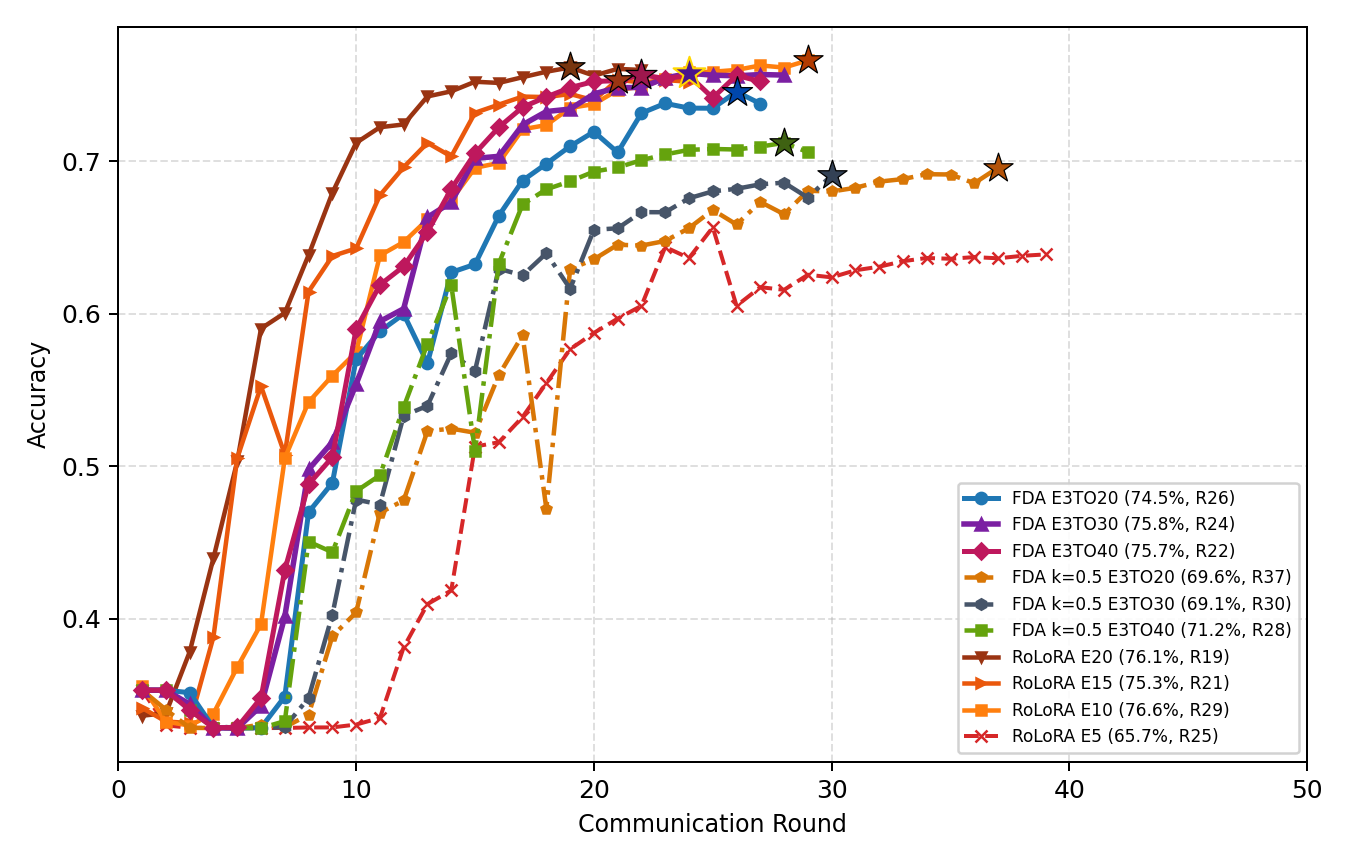
\includegraphics[width=\textwidth,height=4.9cm,keepaspectratio]{figures/telemetry/01_MNLI_C20_R50_LR0.1_1_accuracy.png}
            \vspace{2pt}
            \par{\footnotesize \textbf{(a)} Validation Accuracy}
        \end{minipage}\hfill
        \begin{minipage}[b]{0.485\textwidth}
            \centering
            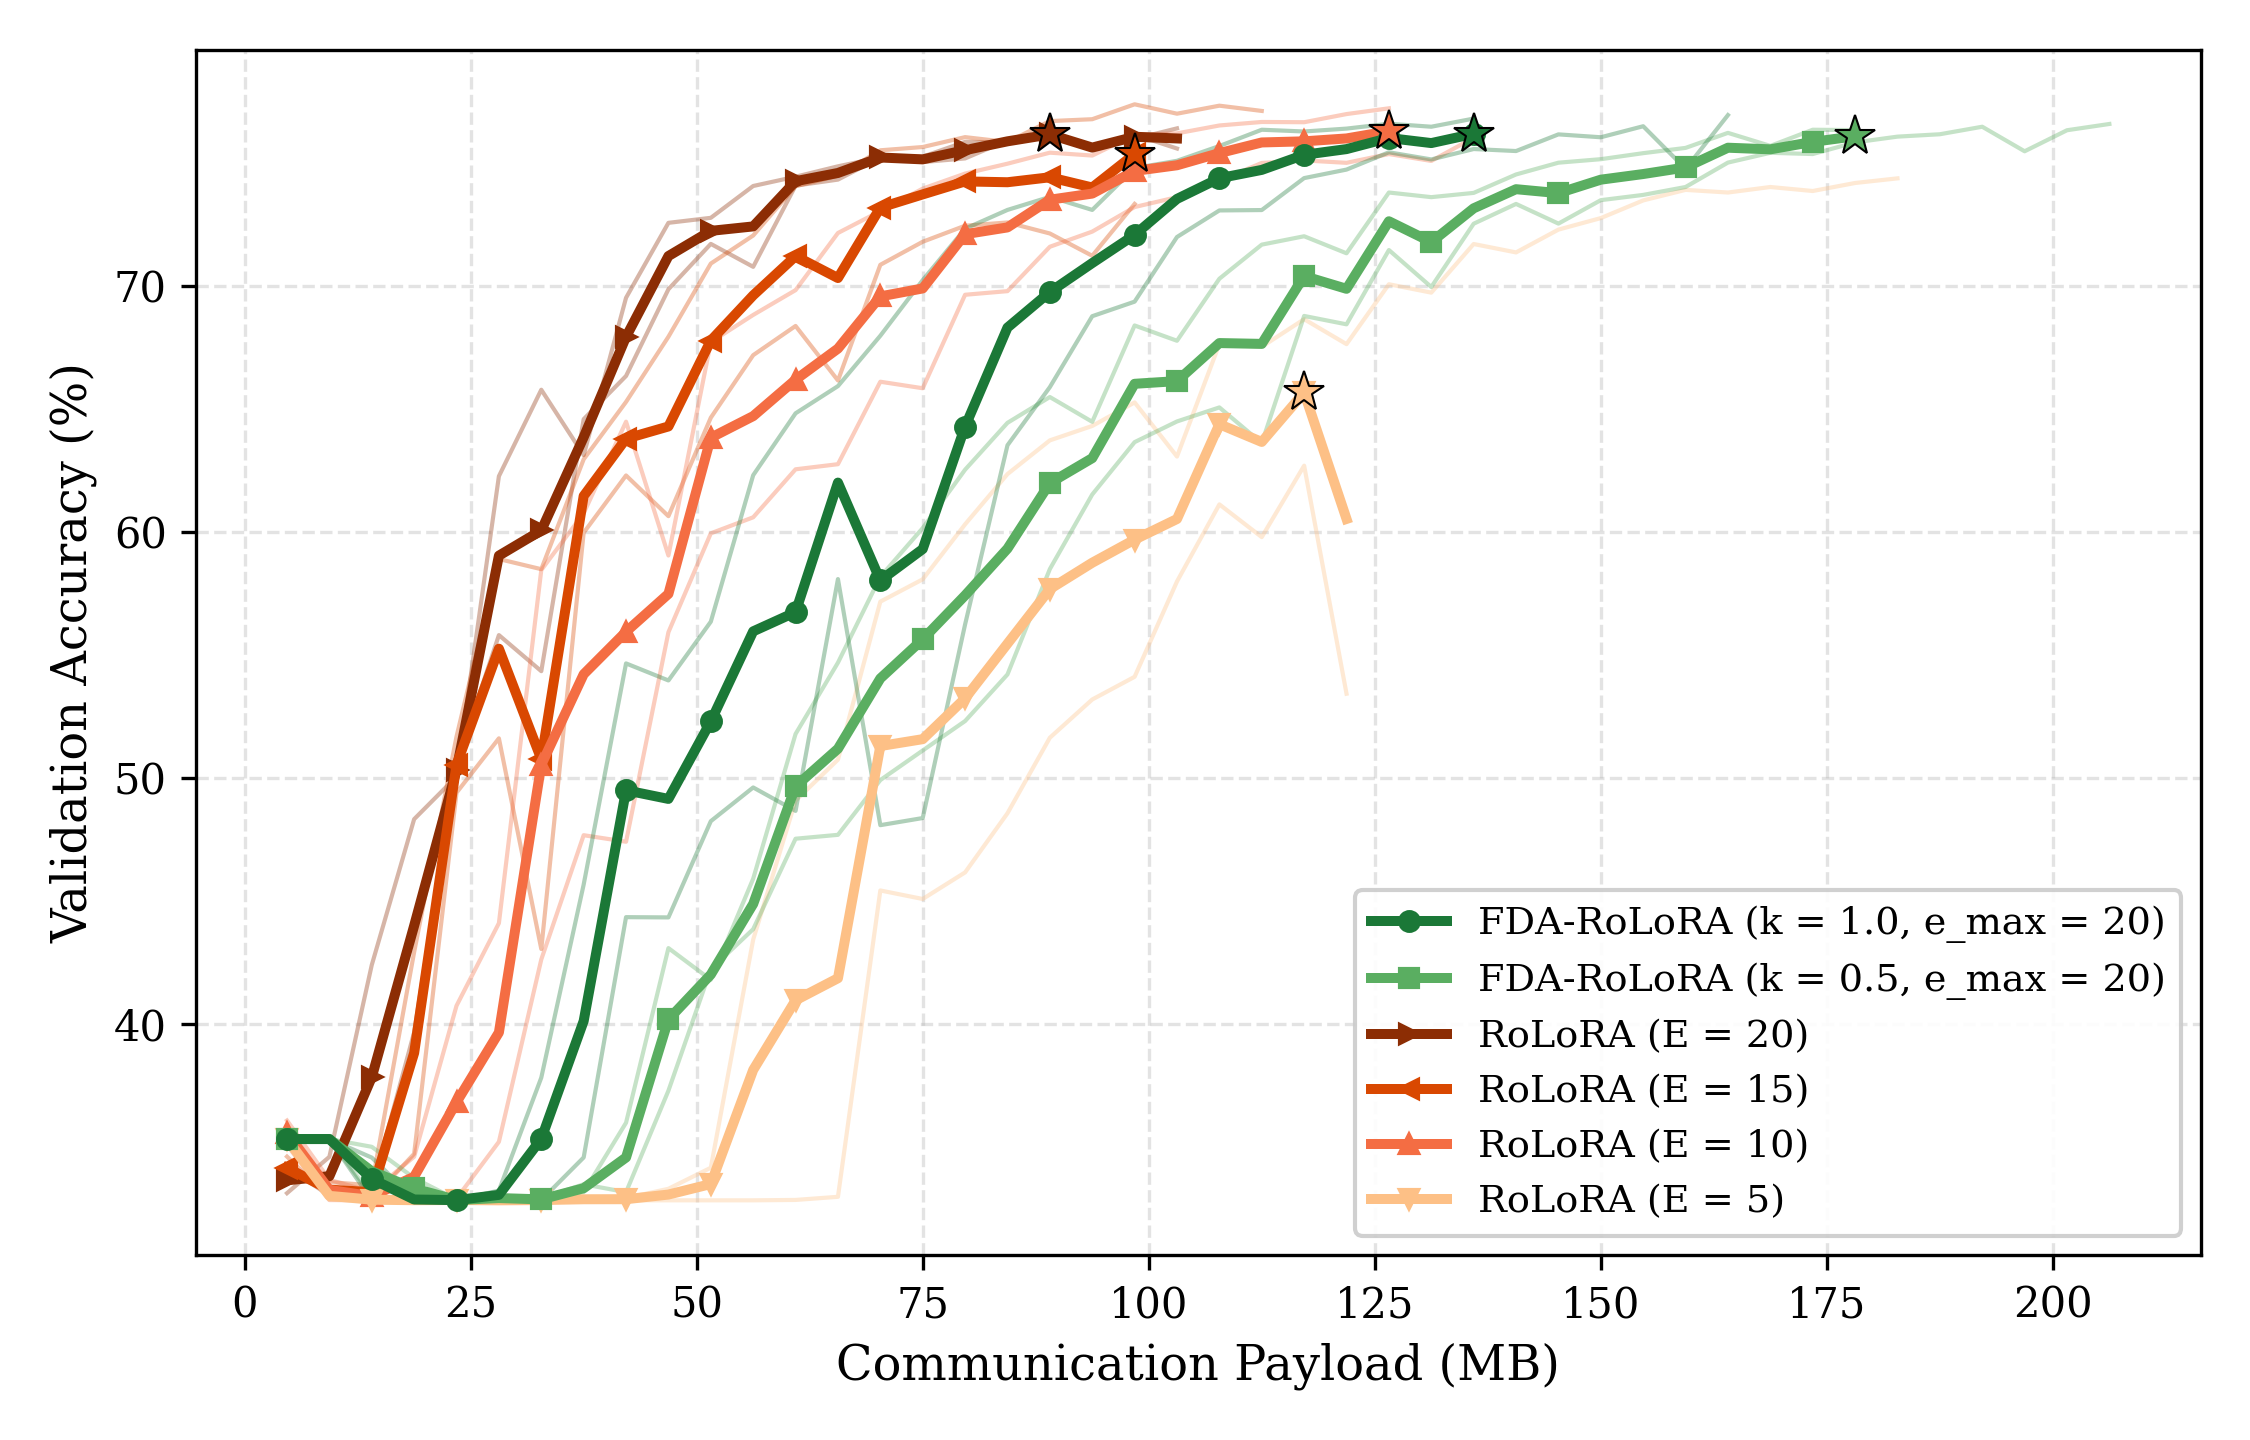
\includegraphics[width=\textwidth,height=4.9cm,keepaspectratio]{figures/telemetry/01_MNLI_C20_R50_LR0.1_4_accuracy_vs_cost.png}
            \vspace{2pt}
            \par{\footnotesize \textbf{(b)} Accuracy vs. Communication (MB)}
        \end{minipage}

        \vspace{0.6em}
        \begin{minipage}[b]{0.485\textwidth}
            \centering
            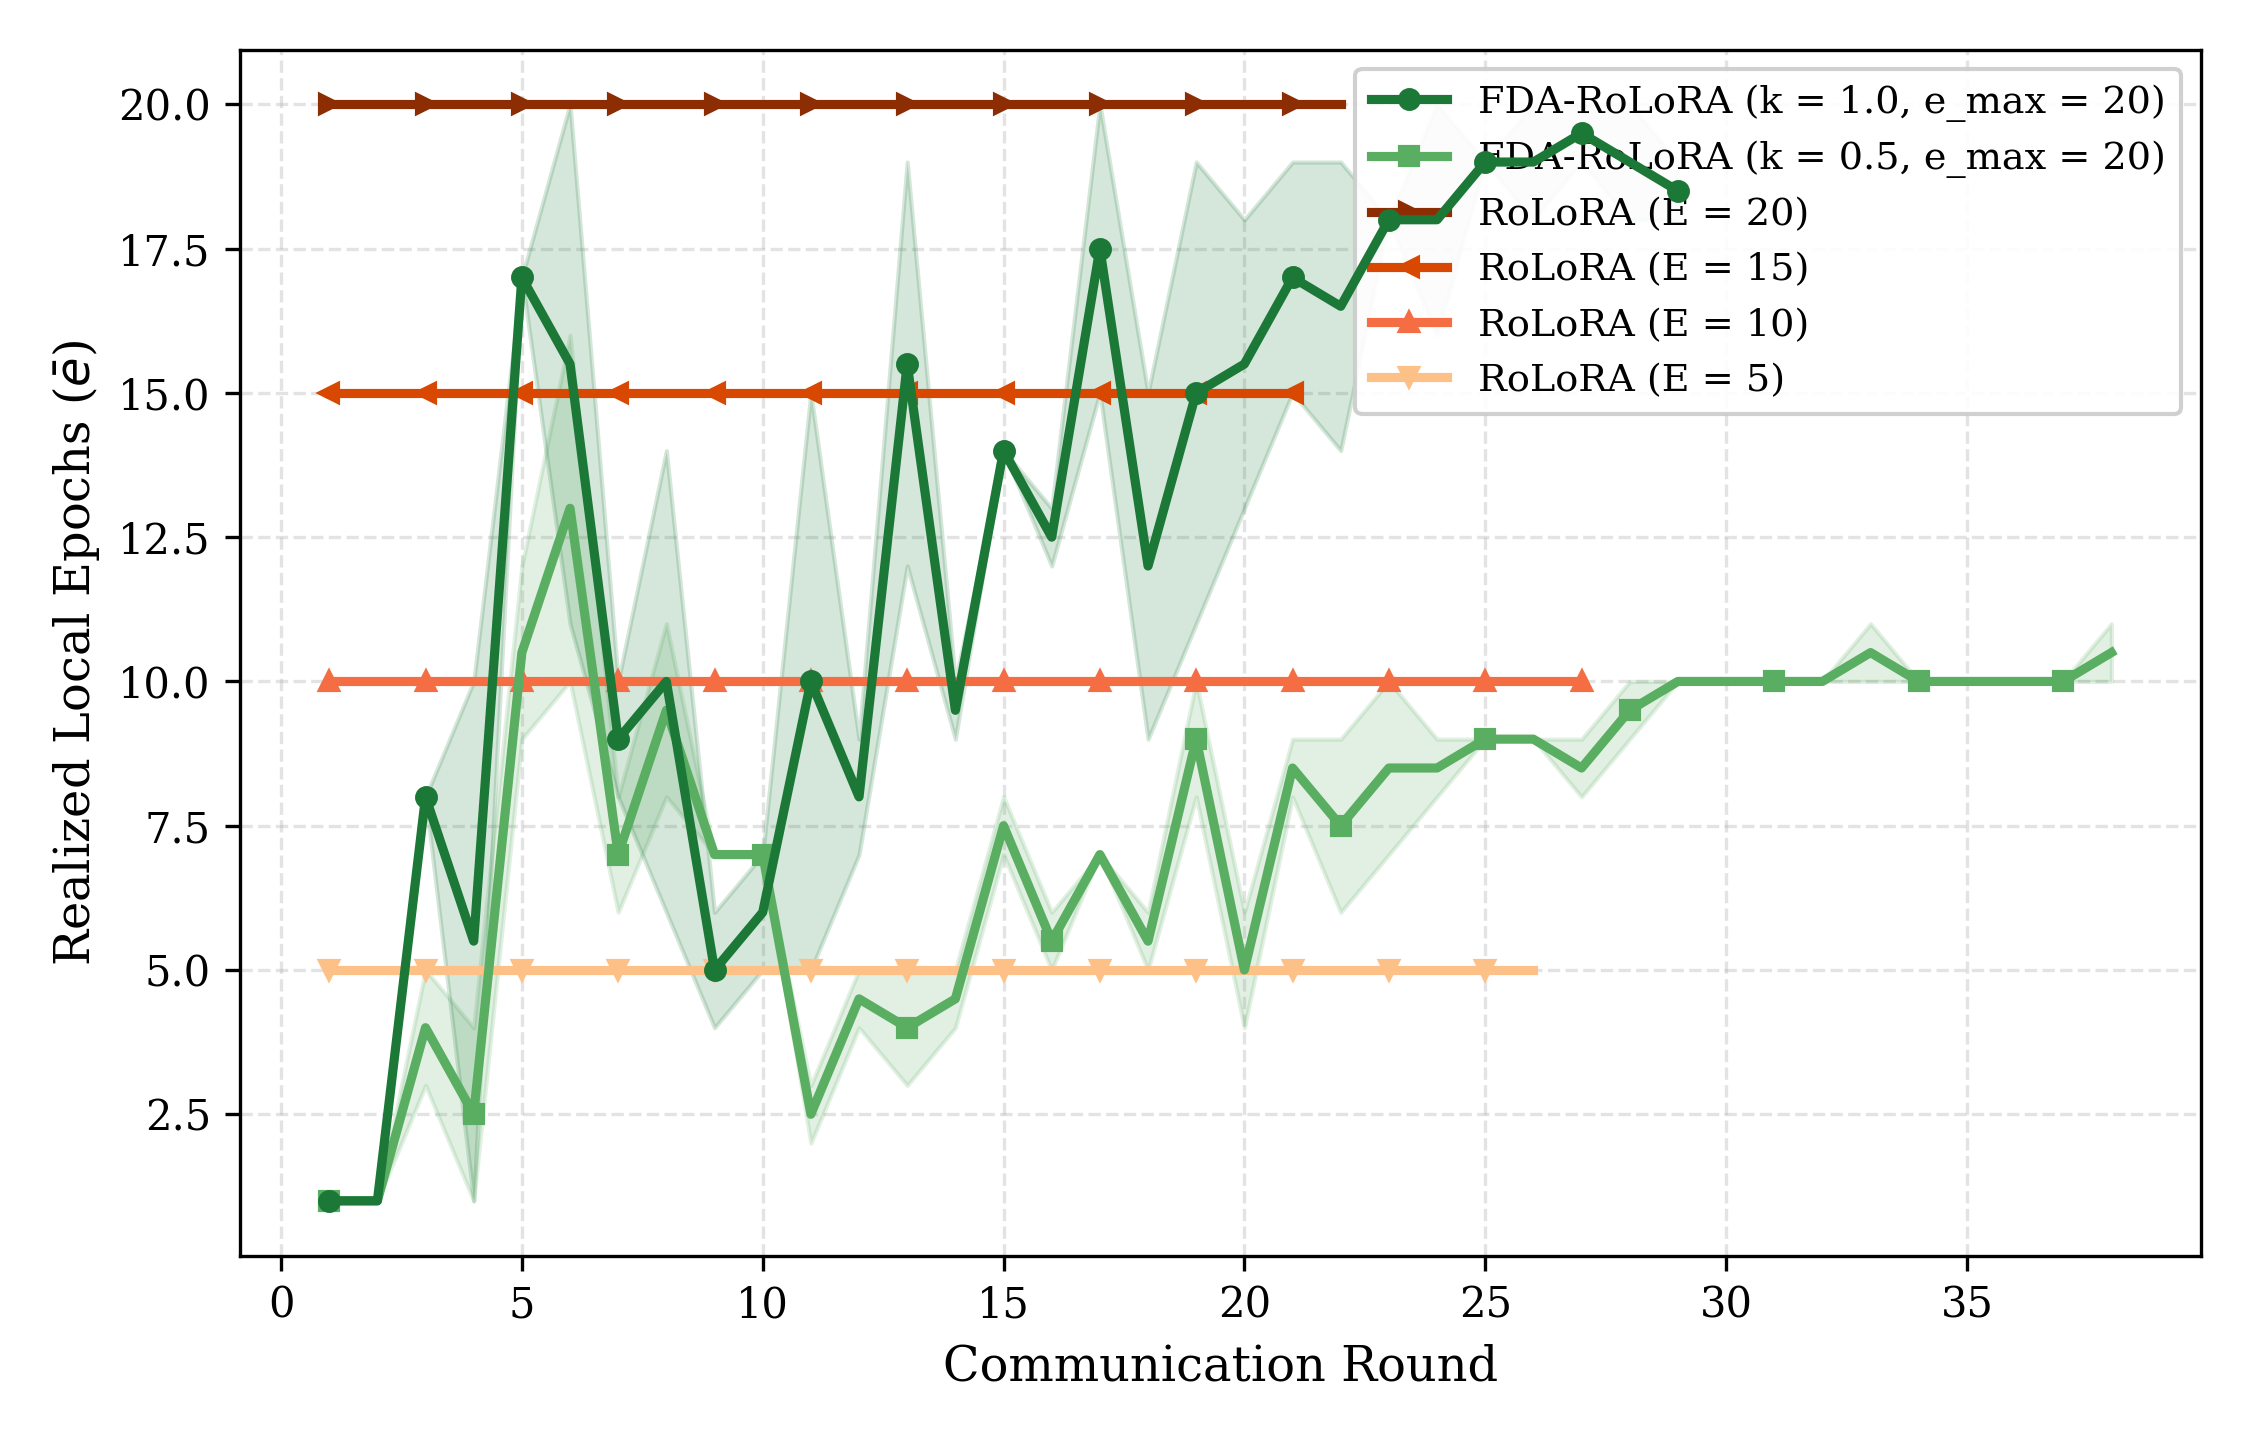
\includegraphics[width=\textwidth,height=4.9cm,keepaspectratio]{figures/telemetry/01_MNLI_C20_R50_LR0.1_2_allocated_epochs.png}
            \vspace{2pt}
            \par{\footnotesize \textbf{(c)} Dynamic Local Epochs ($\bar{e}$)}
        \end{minipage}\hfill
        \begin{minipage}[b]{0.485\textwidth}
            \centering
            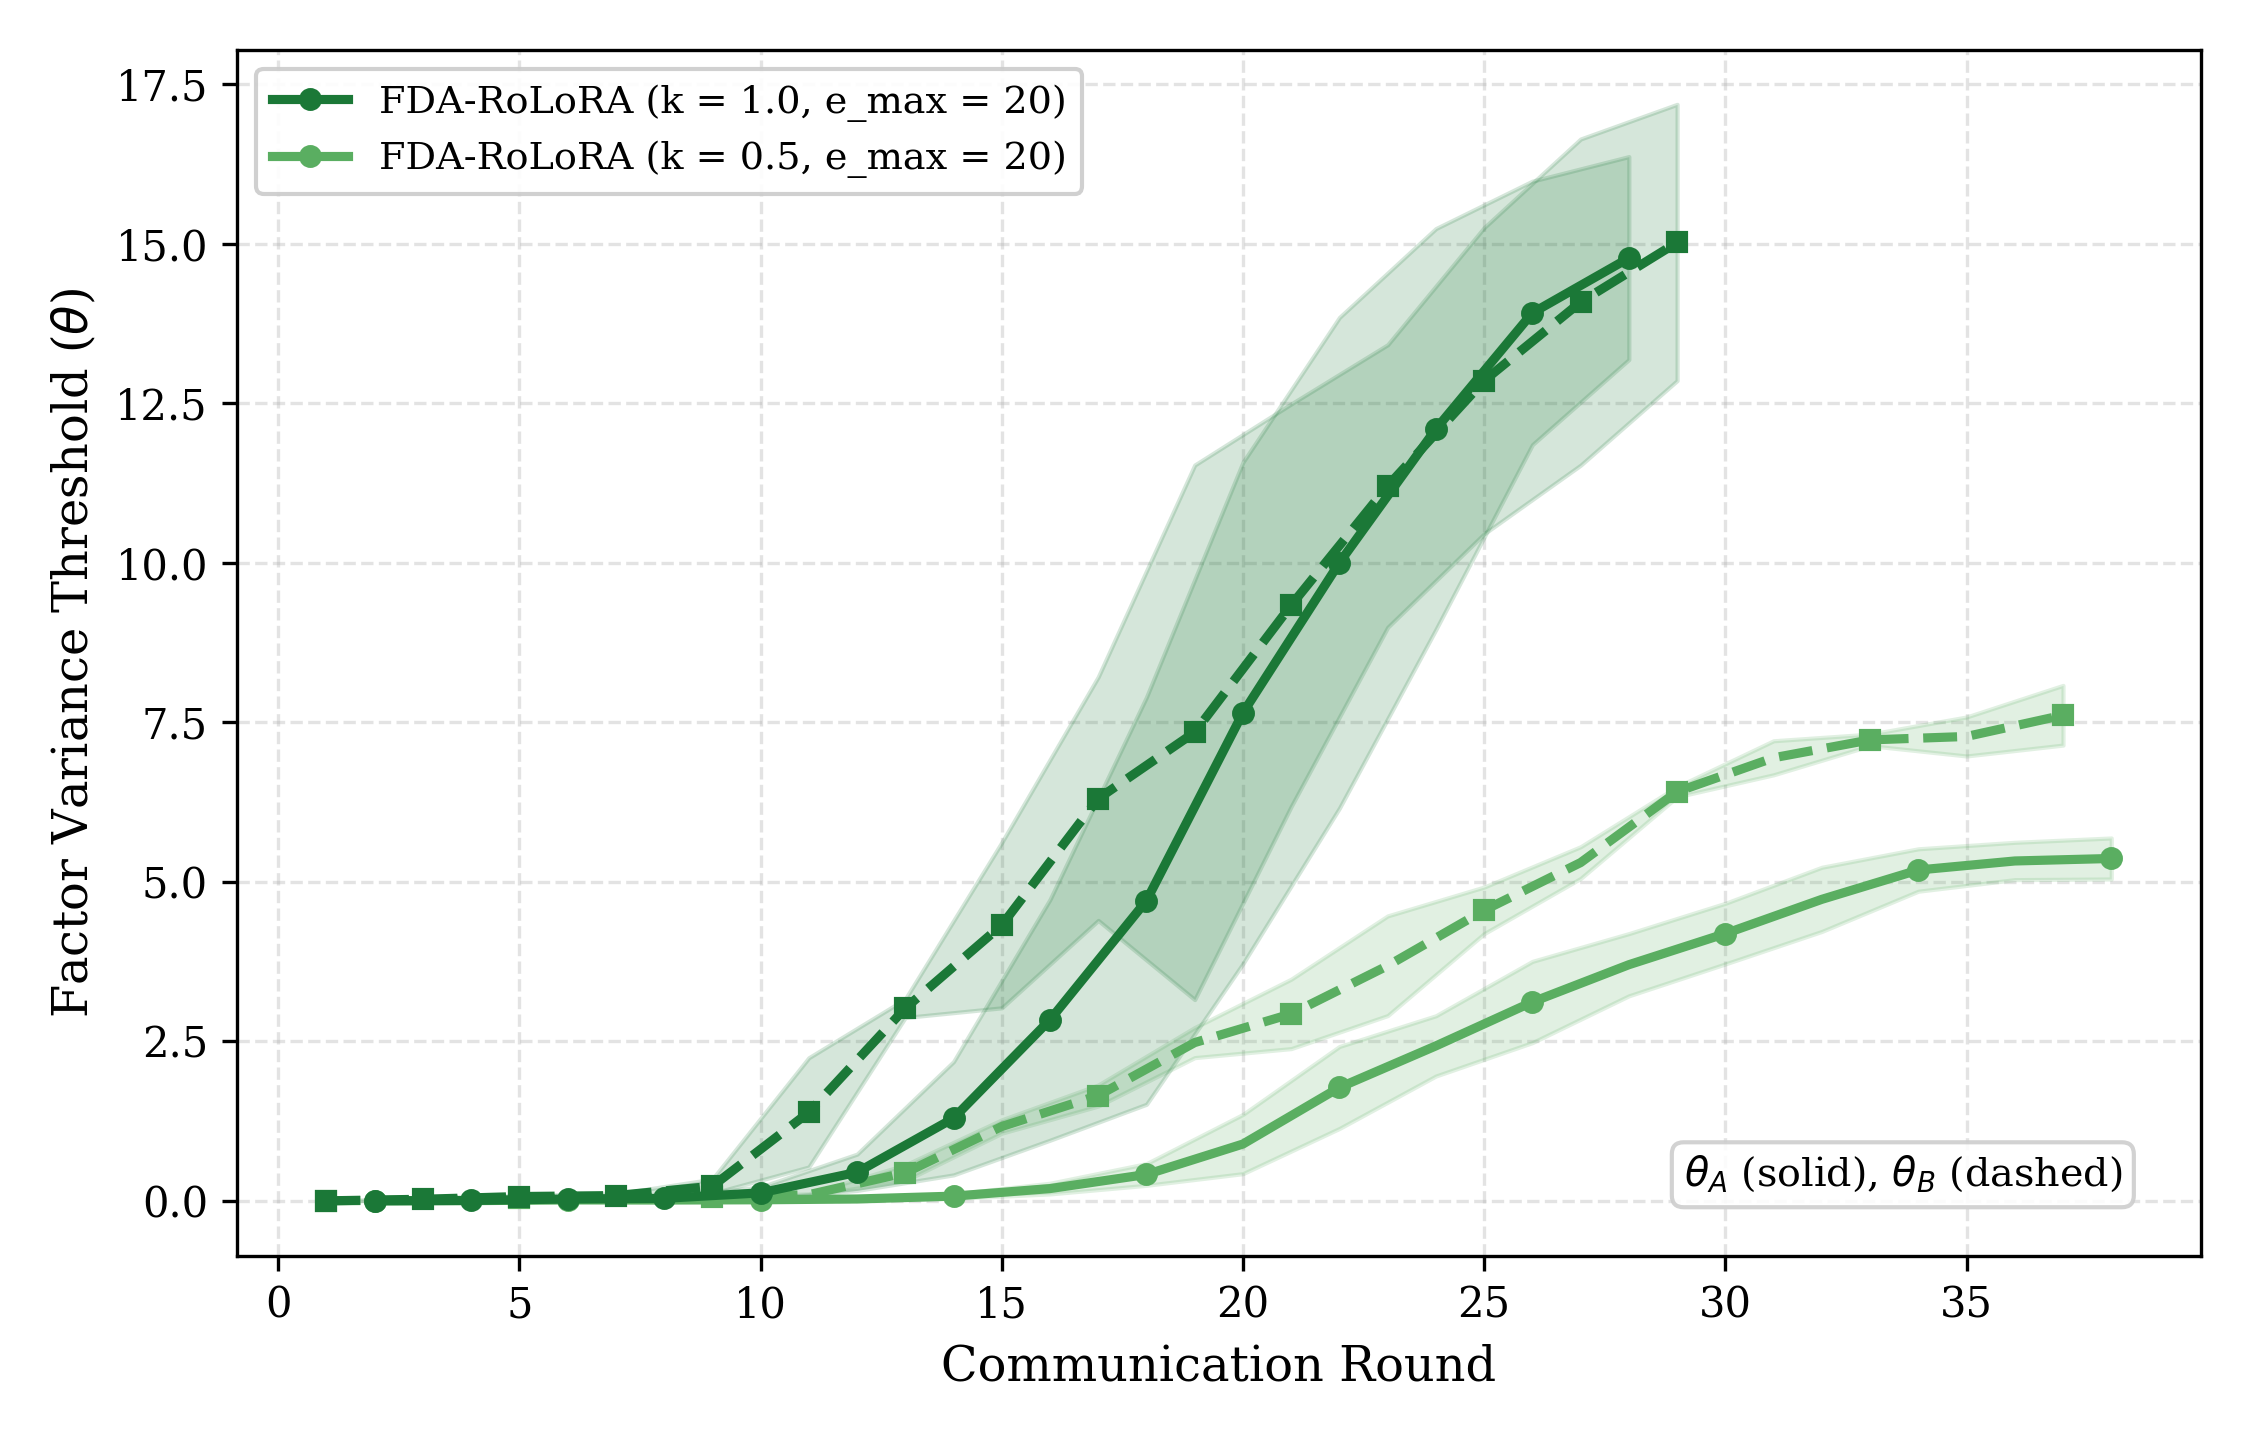
\includegraphics[width=\textwidth,height=4.9cm,keepaspectratio]{figures/telemetry/01_MNLI_C20_R50_LR0.1_5_fda_threshold.png}
            \vspace{2pt}
            \par{\footnotesize \textbf{(d)} Factor Thresholds ($\theta_A, \theta_B$)}
        \end{minipage}

        \vspace{0.6em}
        \begin{minipage}[b]{0.485\textwidth}
            \centering
            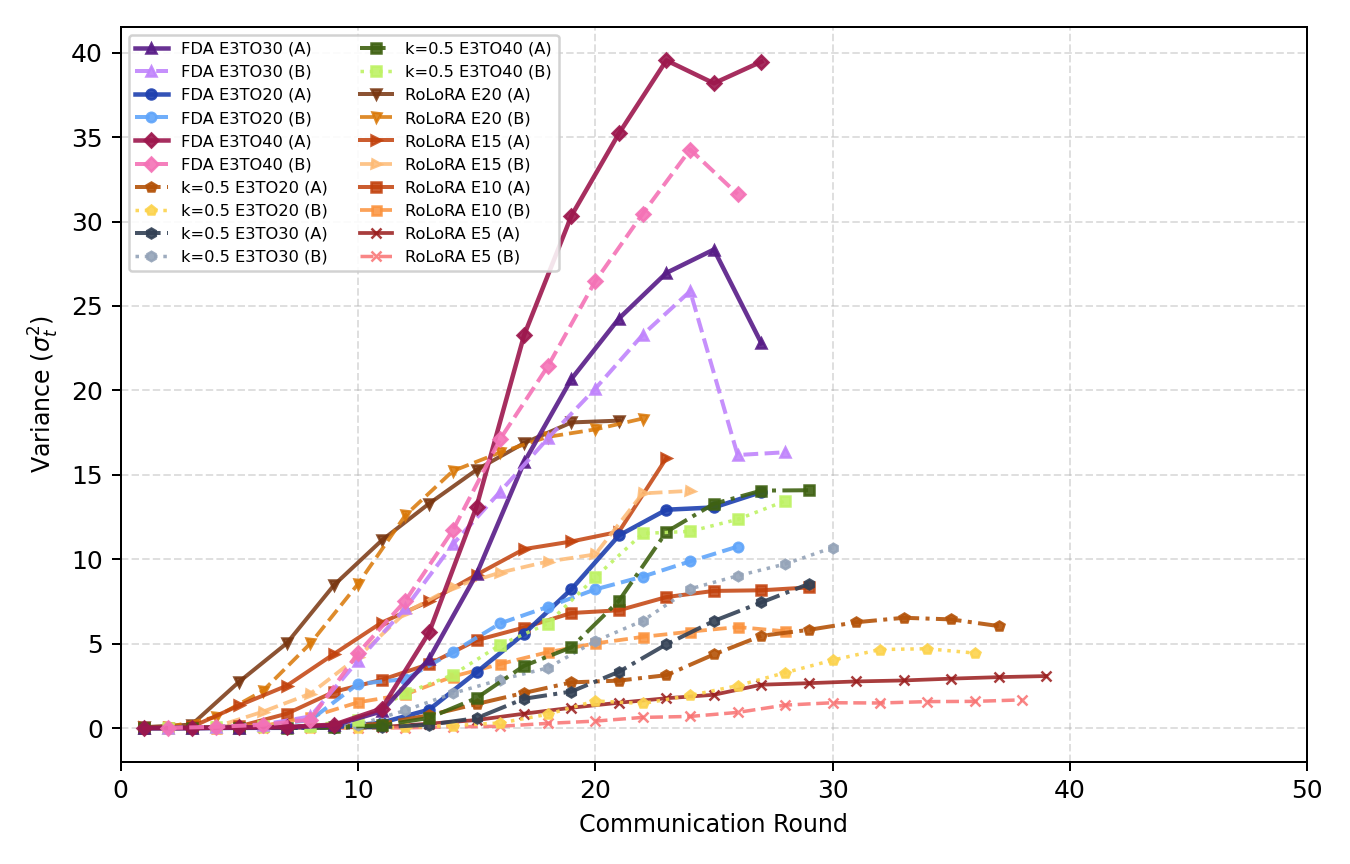
\includegraphics[width=\textwidth,height=4.9cm,keepaspectratio]{figures/telemetry/01_MNLI_C20_R50_LR0.1_3_client_variance.png}
            \vspace{2pt}
            \par{\footnotesize \textbf{(e)} Subspace Coordinate Variance}
        \end{minipage}\hfill
        \begin{minipage}[b]{0.485\textwidth}
            \centering
            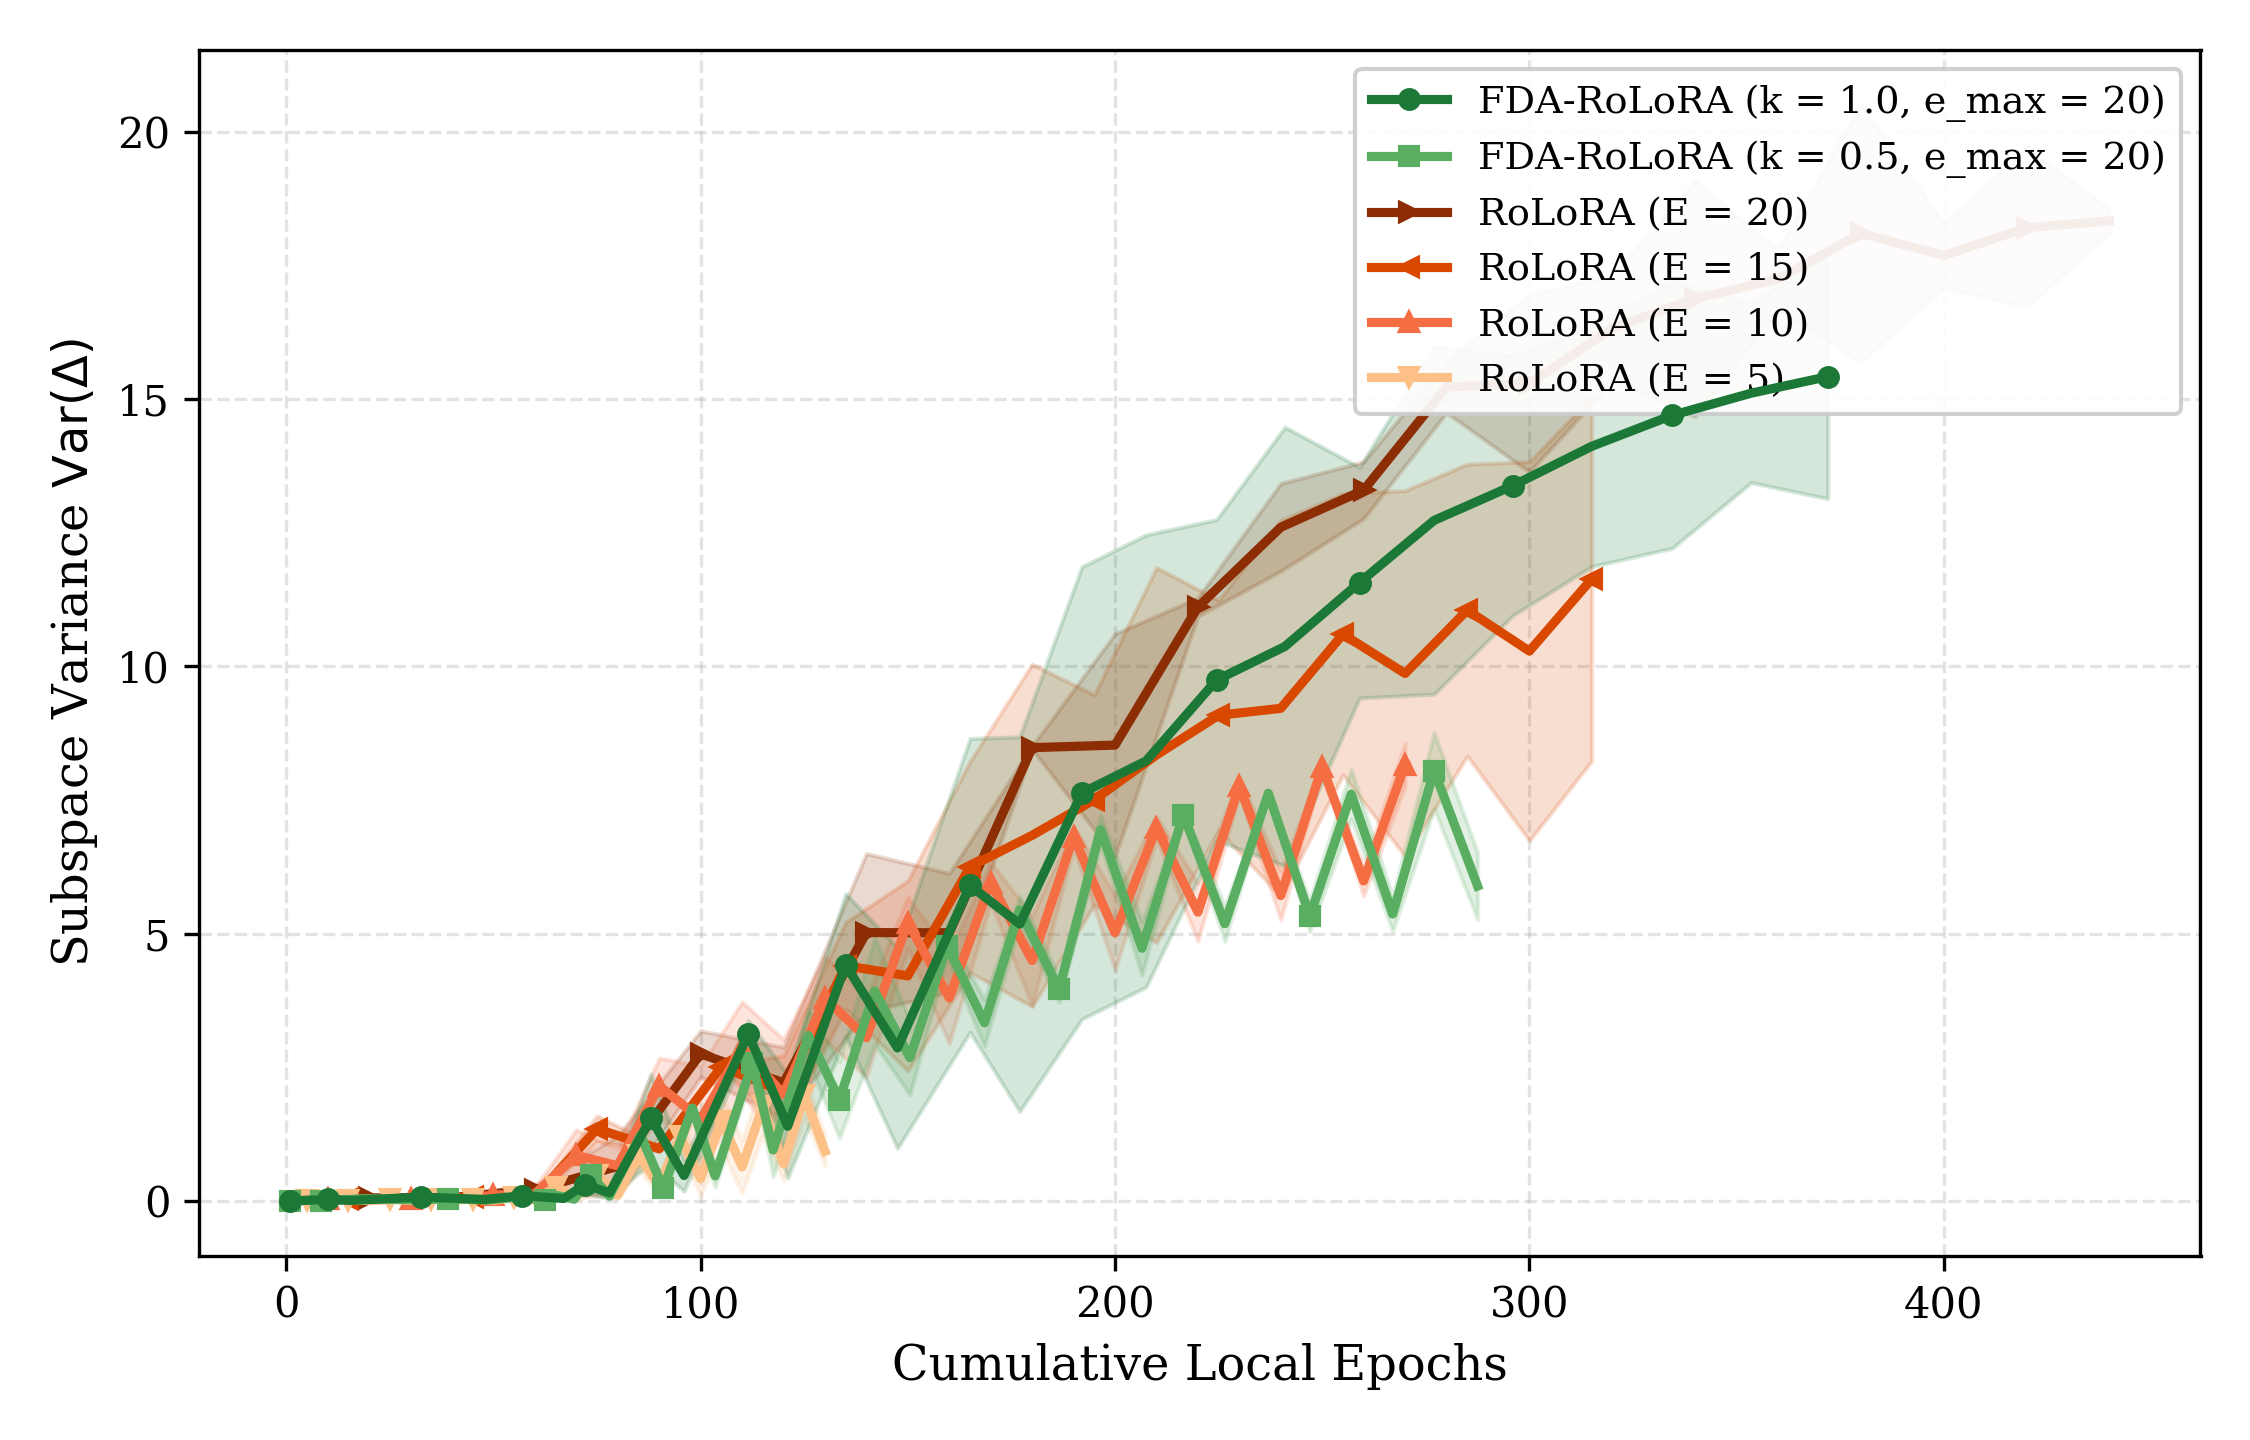
\includegraphics[width=\textwidth,height=4.9cm,keepaspectratio]{figures/telemetry/01_MNLI_C20_R50_LR0.1_6_variance_vs_epoch.png}
            \vspace{2pt}
            \par{\footnotesize \textbf{(f)} Variance vs.\ Cumulative Local Epochs}
        \end{minipage}

        \vspace{0.6em}
        \caption{Multi-panel optimization telemetry on MNLI ($C=20, R_{\max}=50, \eta_c=0.1, \alpha=1000.0$) comparing FDA-RoLoRA against static RoLoRA baselines under homogeneous consensus.}
        \label{fig:telemetry_mnli_c20_iid}
    \end{minipage}%
    }
\end{figure}

\begin{figure}[p]
    \centering
    \makebox[\textwidth][c]{%
    \begin{minipage}{1.06\textwidth}
        \begin{minipage}[b]{0.485\textwidth}
            \centering
            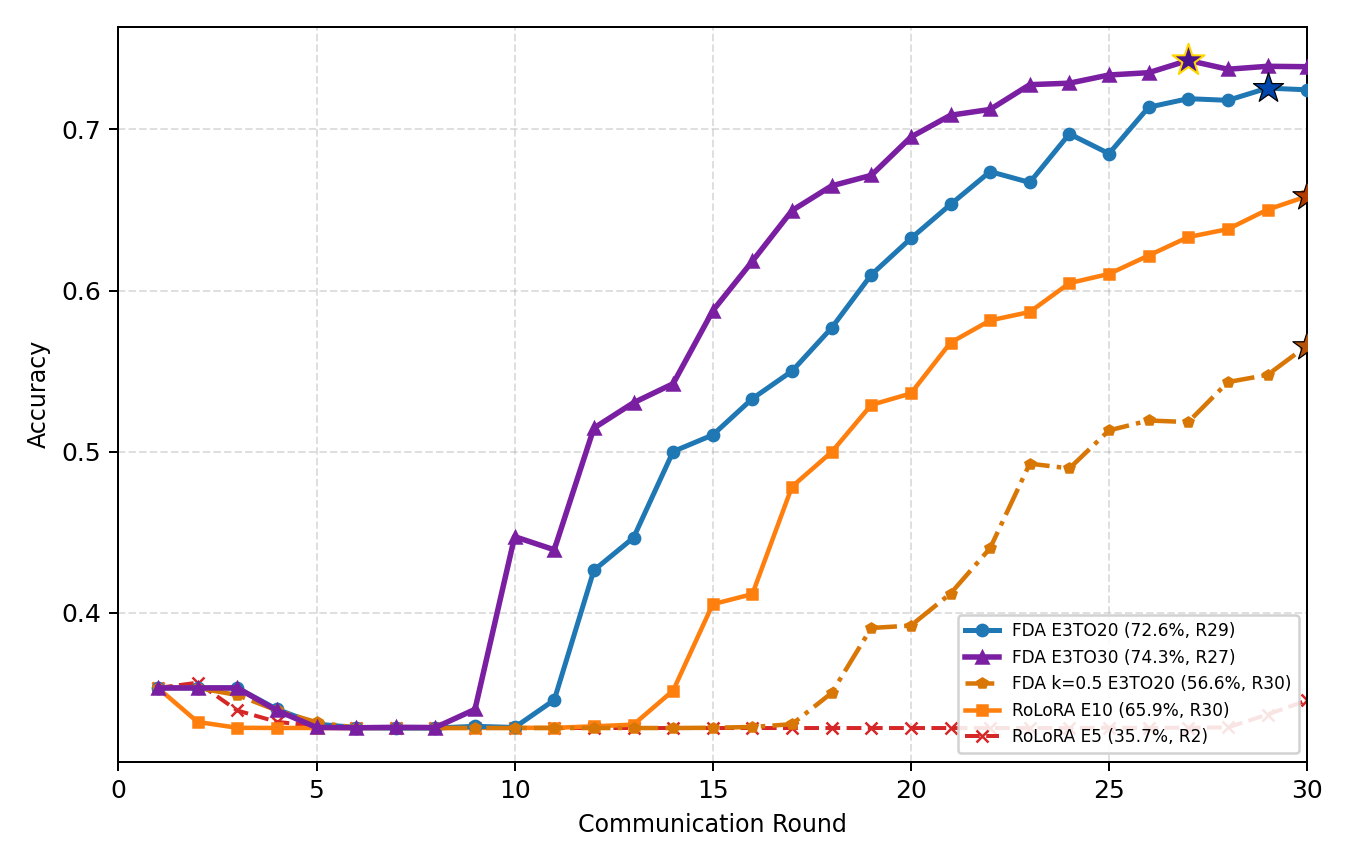
\includegraphics[width=\textwidth,height=4.9cm,keepaspectratio]{figures/telemetry/03_MNLI_C50_R30_LR0.1_1_accuracy.png}
            \vspace{2pt}
            \par{\footnotesize \textbf{(a)} Validation Accuracy}
        \end{minipage}\hfill
        \begin{minipage}[b]{0.485\textwidth}
            \centering
            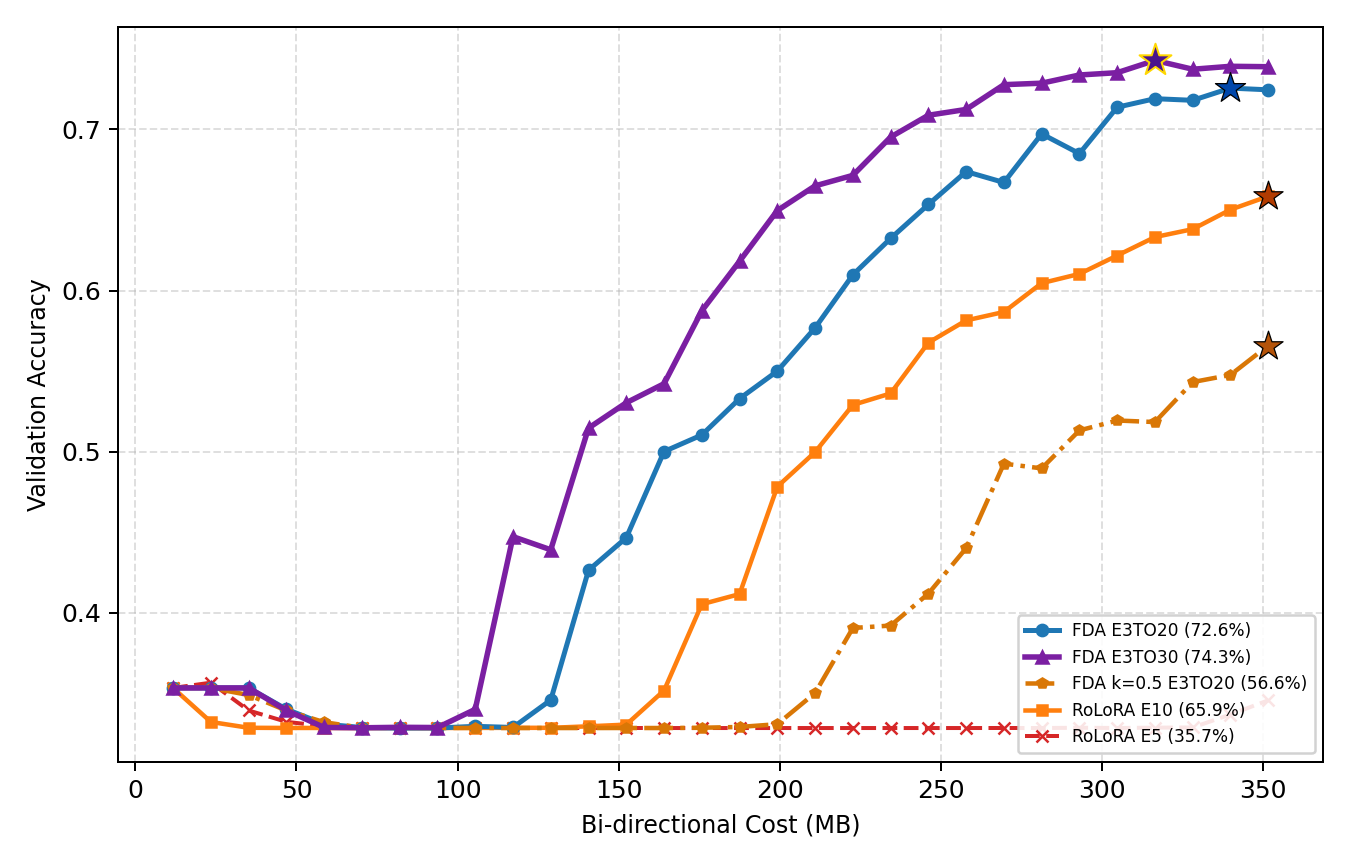
\includegraphics[width=\textwidth,height=4.9cm,keepaspectratio]{figures/telemetry/03_MNLI_C50_R30_LR0.1_4_accuracy_vs_cost.png}
            \vspace{2pt}
            \par{\footnotesize \textbf{(b)} Accuracy vs. Communication (MB)}
        \end{minipage}

        \vspace{0.6em}
        \begin{minipage}[b]{0.485\textwidth}
            \centering
            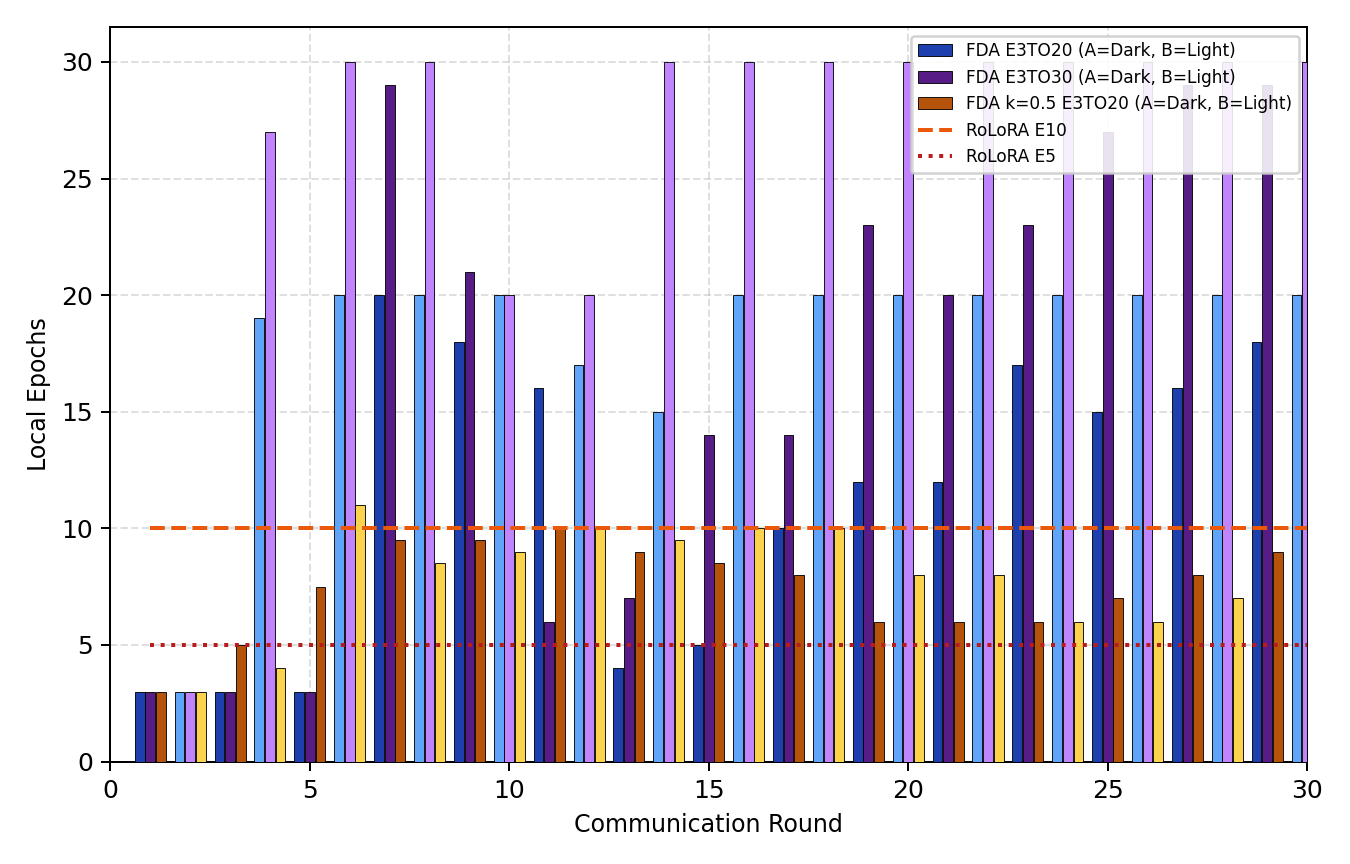
\includegraphics[width=\textwidth,height=4.9cm,keepaspectratio]{figures/telemetry/03_MNLI_C50_R30_LR0.1_2_allocated_epochs.png}
            \vspace{2pt}
            \par{\footnotesize \textbf{(c)} Dynamic Local Epochs ($\bar{e}$)}
        \end{minipage}\hfill
        \begin{minipage}[b]{0.485\textwidth}
            \centering
            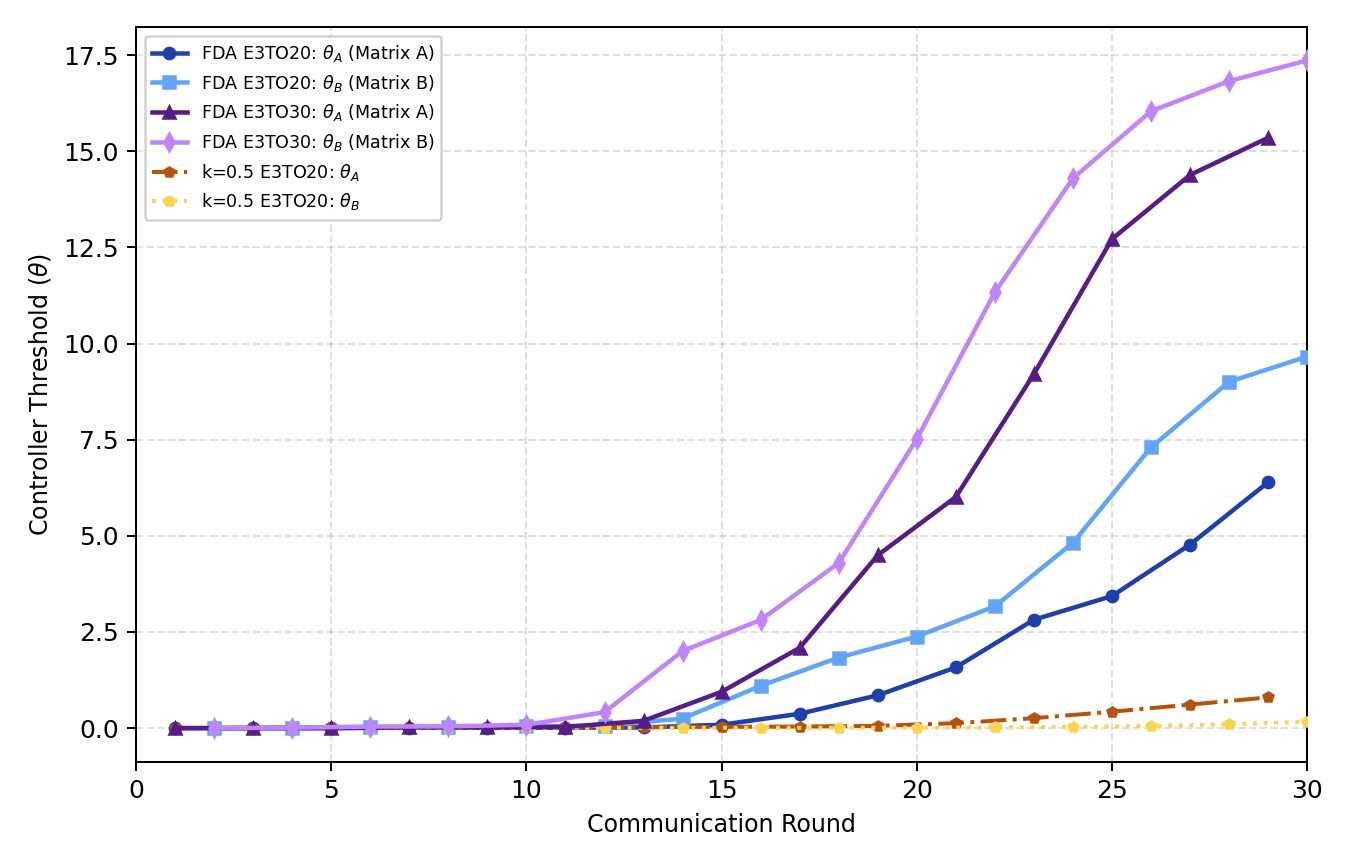
\includegraphics[width=\textwidth,height=4.9cm,keepaspectratio]{figures/telemetry/03_MNLI_C50_R30_LR0.1_5_fda_threshold.png}
            \vspace{2pt}
            \par{\footnotesize \textbf{(d)} Factor Thresholds ($\theta_A, \theta_B$)}
        \end{minipage}

        \vspace{0.6em}
        \begin{minipage}[b]{0.485\textwidth}
            \centering
            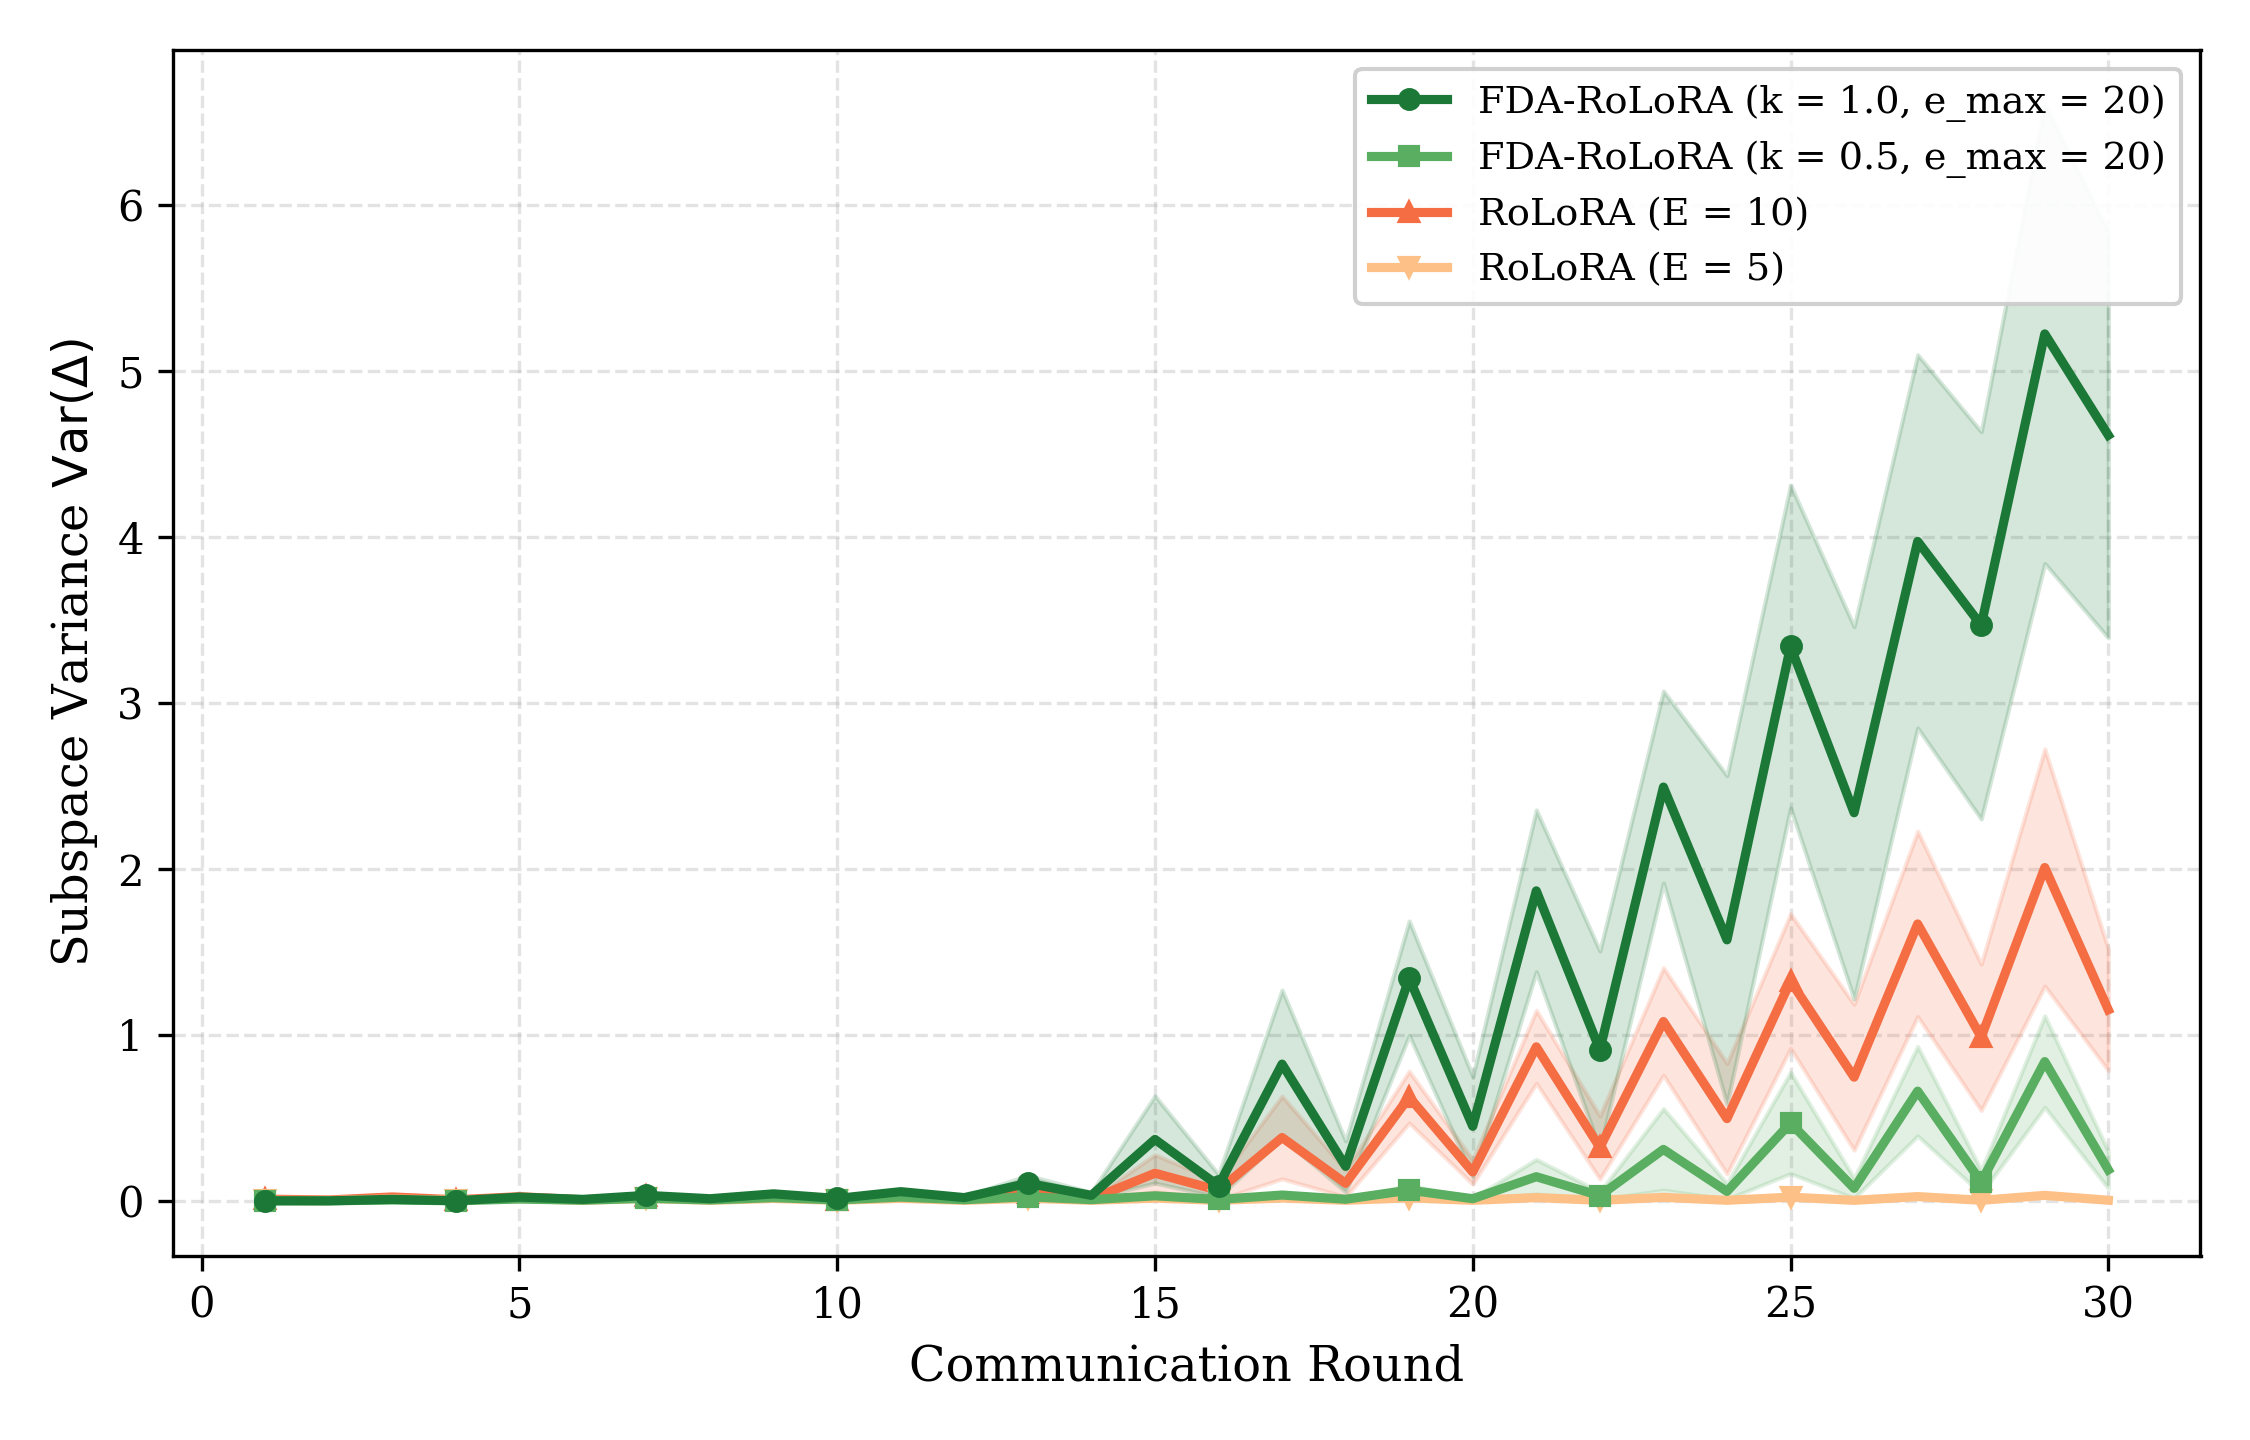
\includegraphics[width=\textwidth,height=4.9cm,keepaspectratio]{figures/telemetry/03_MNLI_C50_R30_LR0.1_3_client_variance.png}
            \vspace{2pt}
            \par{\footnotesize \textbf{(e)} Subspace Coordinate Variance}
        \end{minipage}\hfill
        \begin{minipage}[b]{0.485\textwidth}
            \centering
            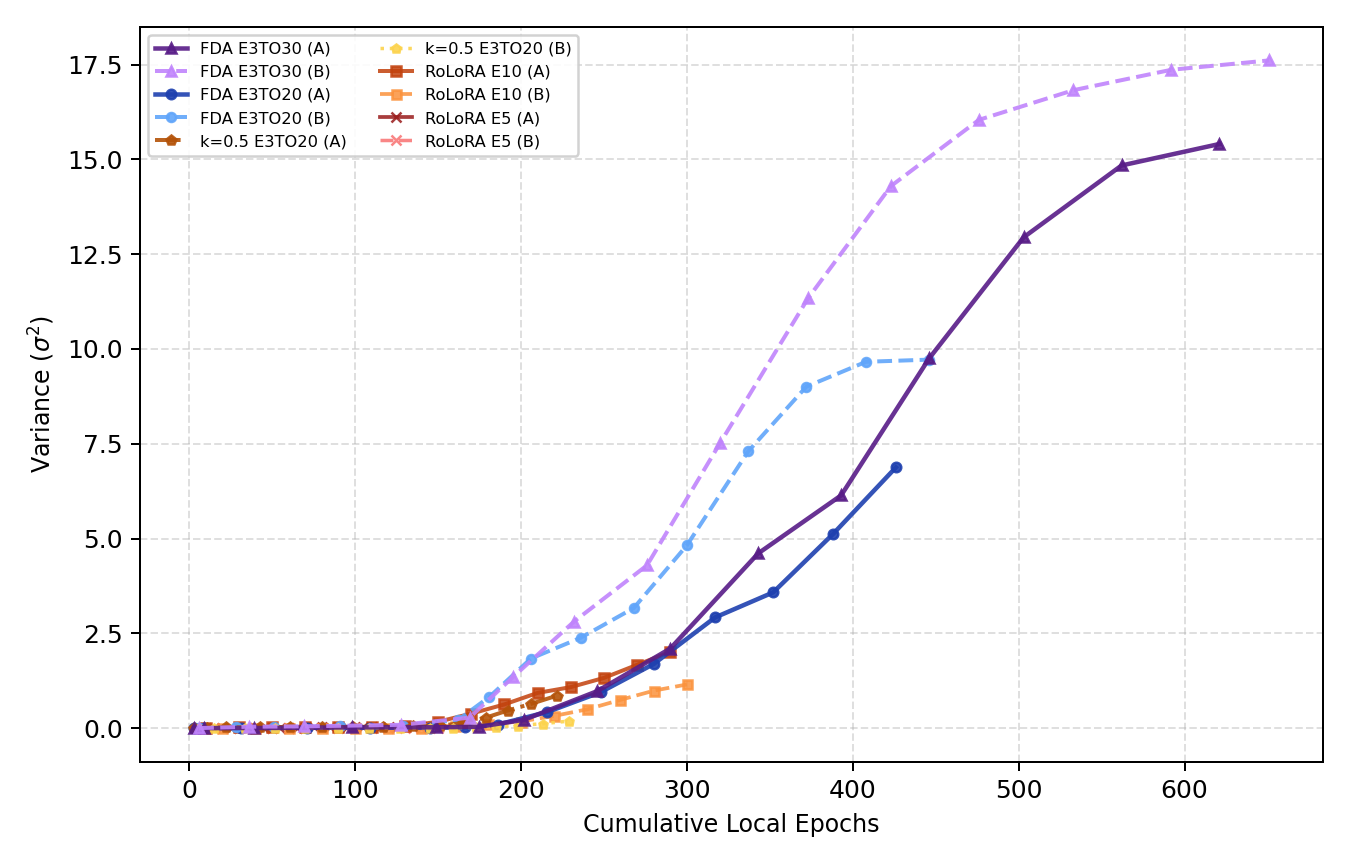
\includegraphics[width=\textwidth,height=4.9cm,keepaspectratio]{figures/telemetry/03_MNLI_C50_R30_LR0.1_6_variance_vs_epoch.png}
            \vspace{2pt}
            \par{\footnotesize \textbf{(f)} Variance vs.\ Cumulative Local Epochs}
        \end{minipage}

        \vspace{0.6em}
        \caption{Multi-panel optimization telemetry on MNLI ($C=50, R_{\max}=30, \eta_c=0.1, \alpha=1000.0$) under expanded cohort scale $C=50$.}
        \label{fig:telemetry_mnli_c50_iid}
    \end{minipage}%
    }
\end{figure}

\paragraph{QNLI:}
Figures~\ref{fig:telemetry_qnli_c20_iid} and \ref{fig:telemetry_qnli_c50_iid} depict optimization dynamics on binary question-answering inference under homogeneous consensus across the six telemetry panels. On $C=20$ (Figure~\ref{fig:telemetry_qnli_c20_iid}), FDA-RoLoRA ($k=1.0$) reaches a peak validation accuracy of $83.14\%$ (Panel a), compared with $81.83\%$ for RoLoRA $E=10$. However, it uses more communication ($77.3\,\text{MB}$ vs.\ $46.9\,\text{MB}$), and its final accuracy ($67.63 \pm 22.28\%$) is lower and less stable than its peak, because one seed ended at $51.9\%$. Dynamic local epochs (Panel c) stabilize at $\bar{e} = 9.85$ per round under $k=1.0$ (and $\bar{e} = 6.91$ under $k=0.5$), below the $k=1.0$ setpoint of 20. Threshold telemetry (Panel d) shows stable monotonic adaptation, preserving separate operational scales for $\theta_A$ and $\theta_B$. Drift variance at round synchronization (Panel e) is kept minimal ($\bar{\nu} \approx 1.11$).

On scaled cohorts of $C=50$ clients (Figure~\ref{fig:telemetry_qnli_c50_iid}), FDA-RoLoRA ($k=1.0$) reaches competitive peak accuracy ($82.77\%$) and triggers early stopping at round 21 ($246.1\,\text{MB}$) versus 24.5 rounds ($287.1\,\text{MB}$) for static RoLoRA $E=10$ (Panel a \& b). Inter-client drift variance (Panel e) averages only $\bar{\nu} = 0.707$.
\begin{figure}[p]
    \centering
    \makebox[\textwidth][c]{%
    \begin{minipage}{1.06\textwidth}
        \begin{minipage}[b]{0.485\textwidth}
            \centering
            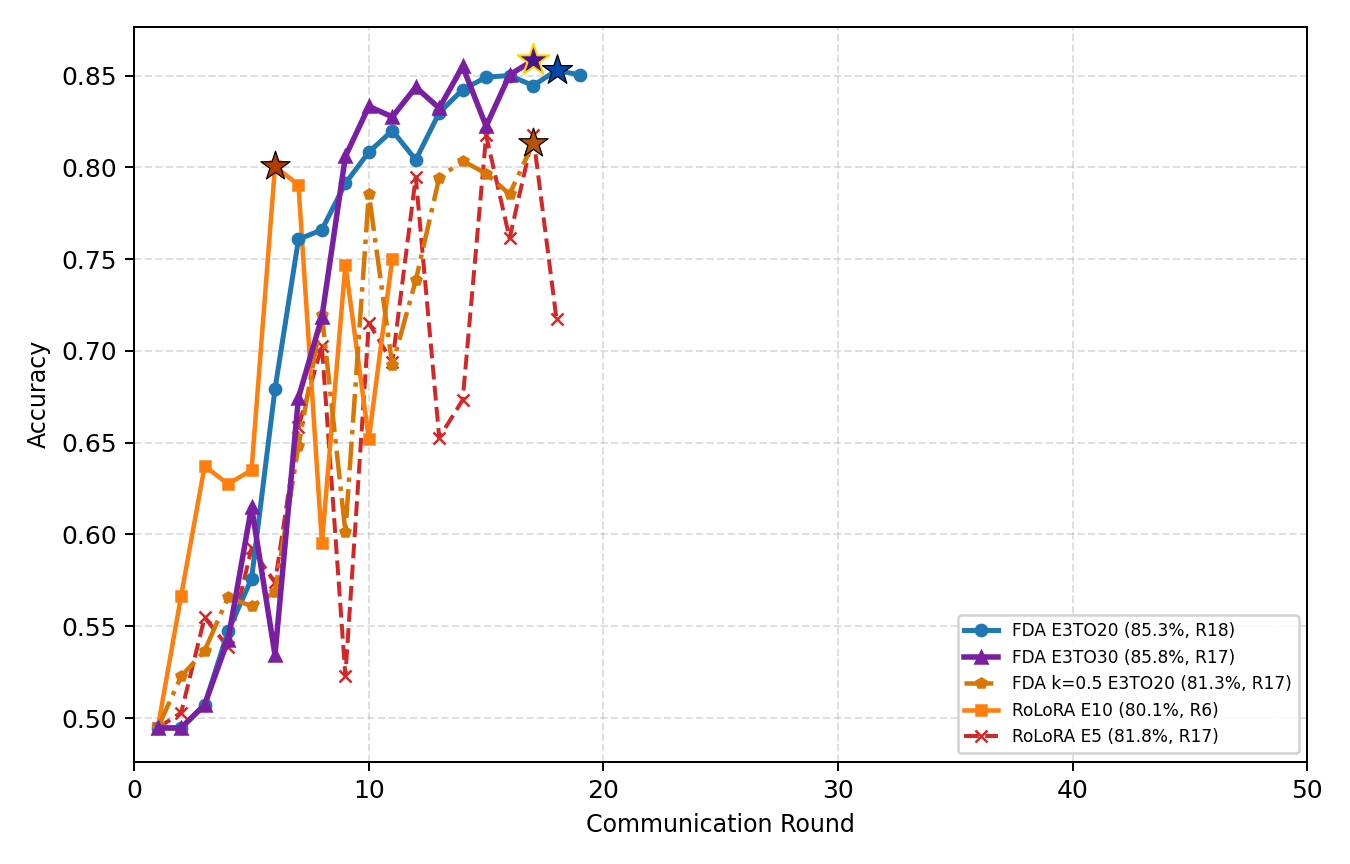
\includegraphics[width=\textwidth,height=4.9cm,keepaspectratio]{figures/telemetry/05_QNLI_C20_R50_LR0.1_1_accuracy.png}
            \vspace{2pt}
            \par{\footnotesize \textbf{(a)} Validation Accuracy}
        \end{minipage}\hfill
        \begin{minipage}[b]{0.485\textwidth}
            \centering
            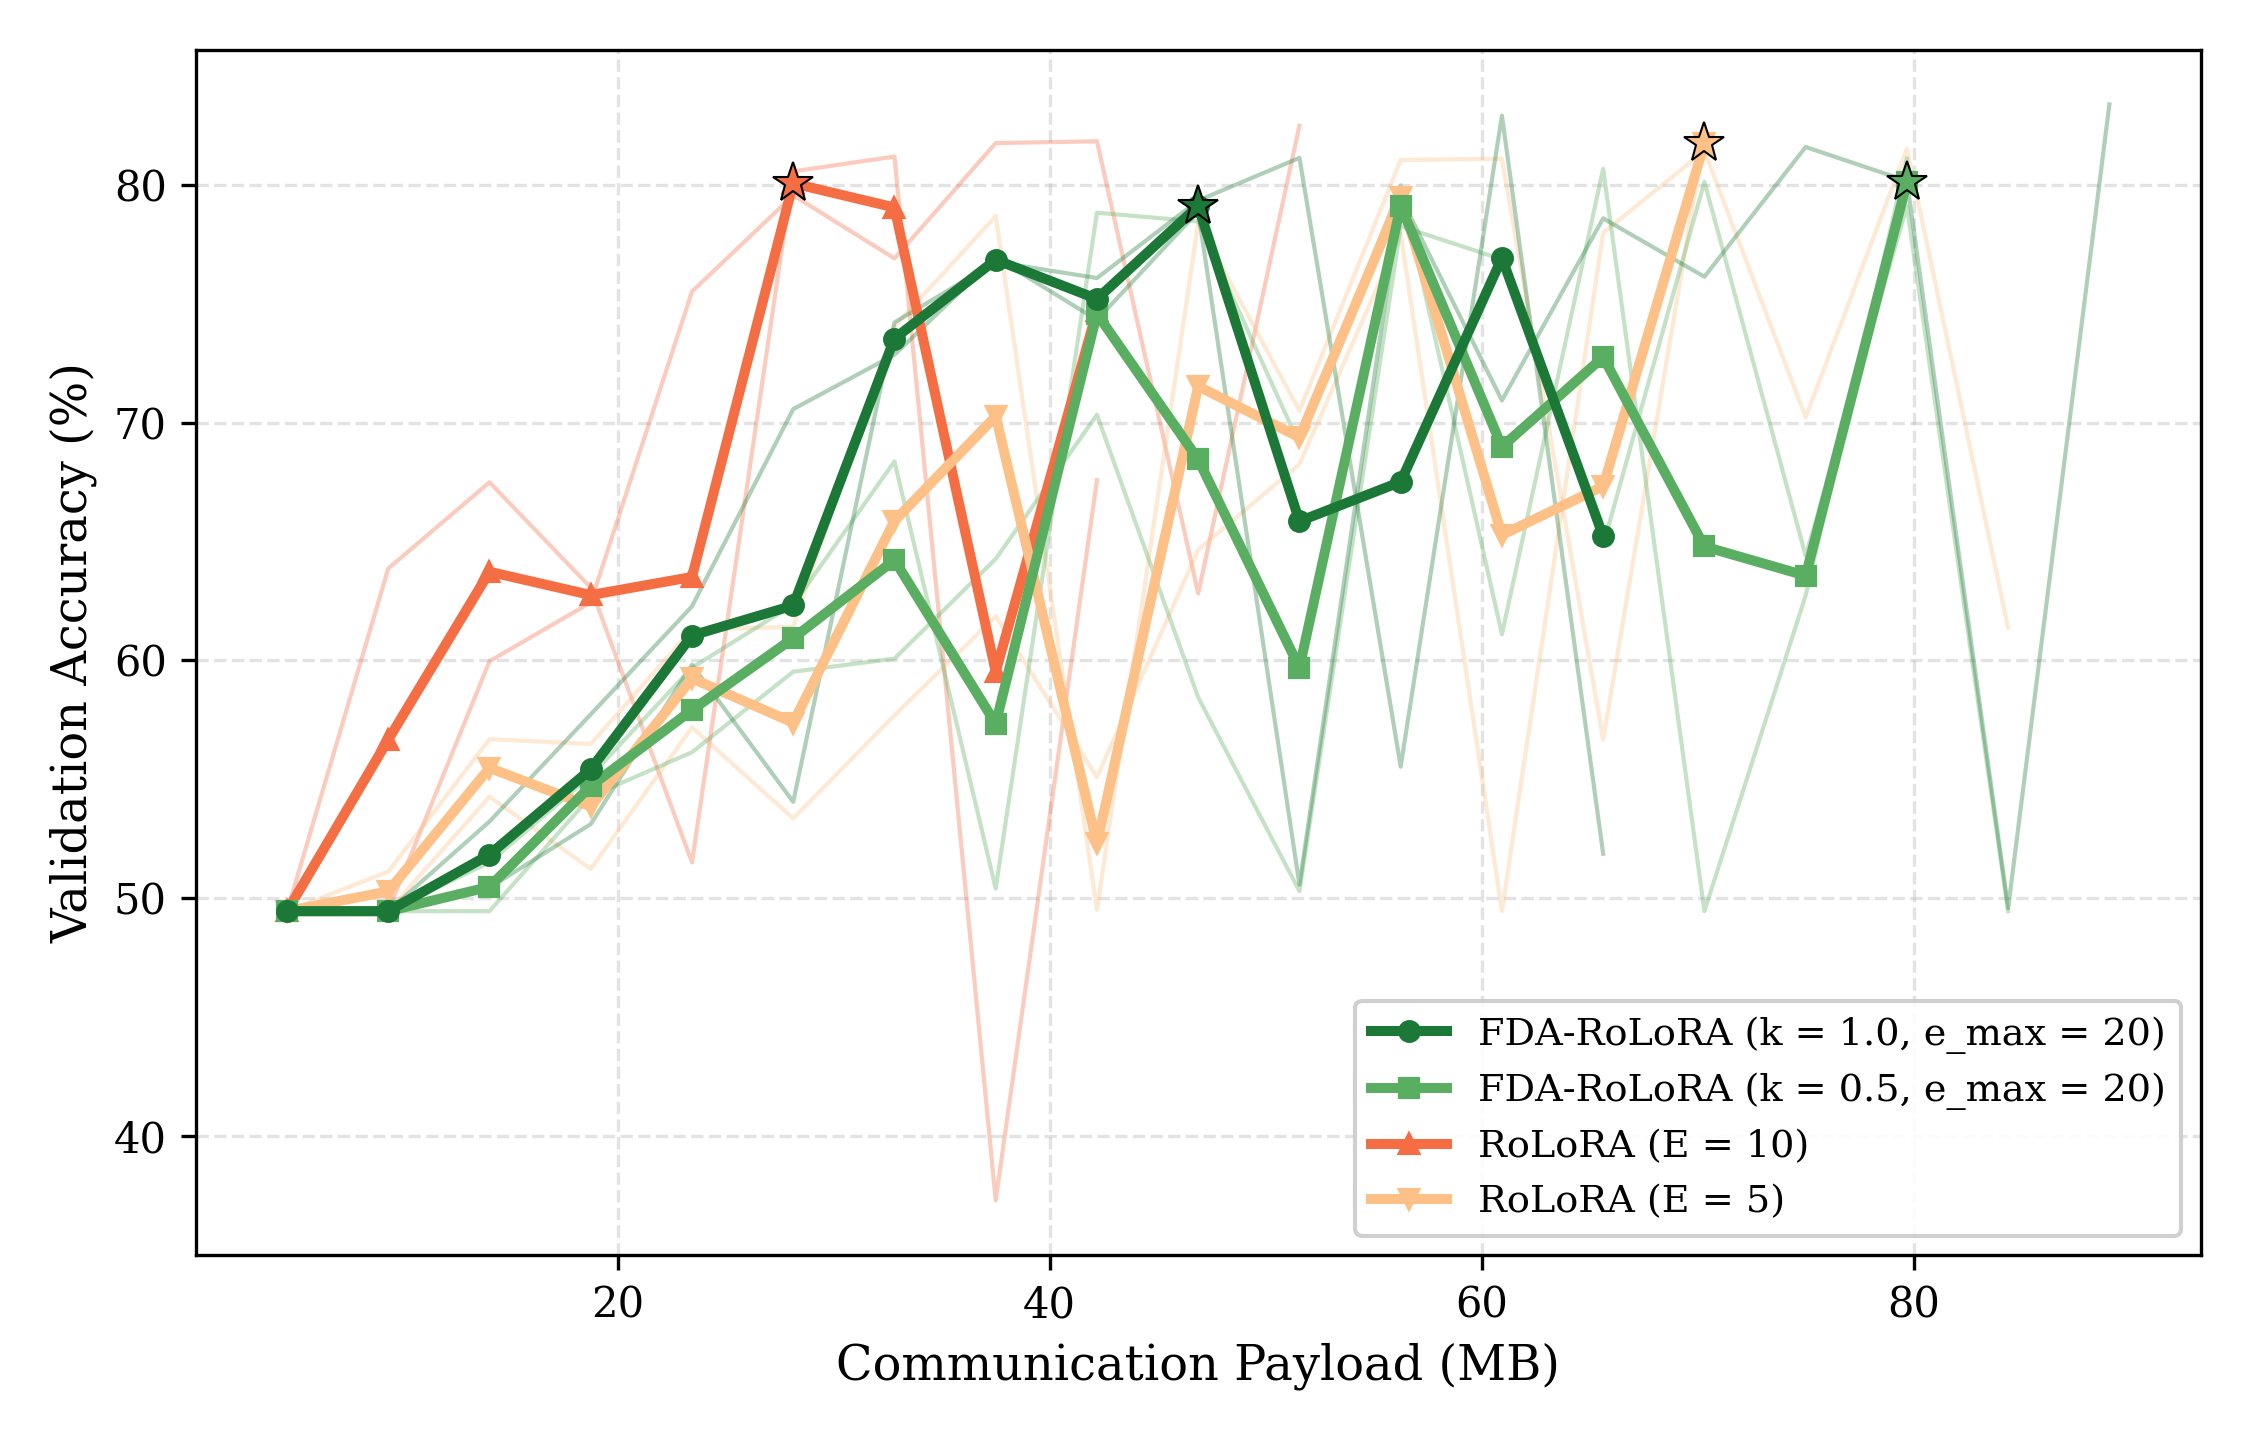
\includegraphics[width=\textwidth,height=4.9cm,keepaspectratio]{figures/telemetry/05_QNLI_C20_R50_LR0.1_4_accuracy_vs_cost.png}
            \vspace{2pt}
            \par{\footnotesize \textbf{(b)} Accuracy vs. Communication (MB)}
        \end{minipage}

        \vspace{0.6em}
        \begin{minipage}[b]{0.485\textwidth}
            \centering
            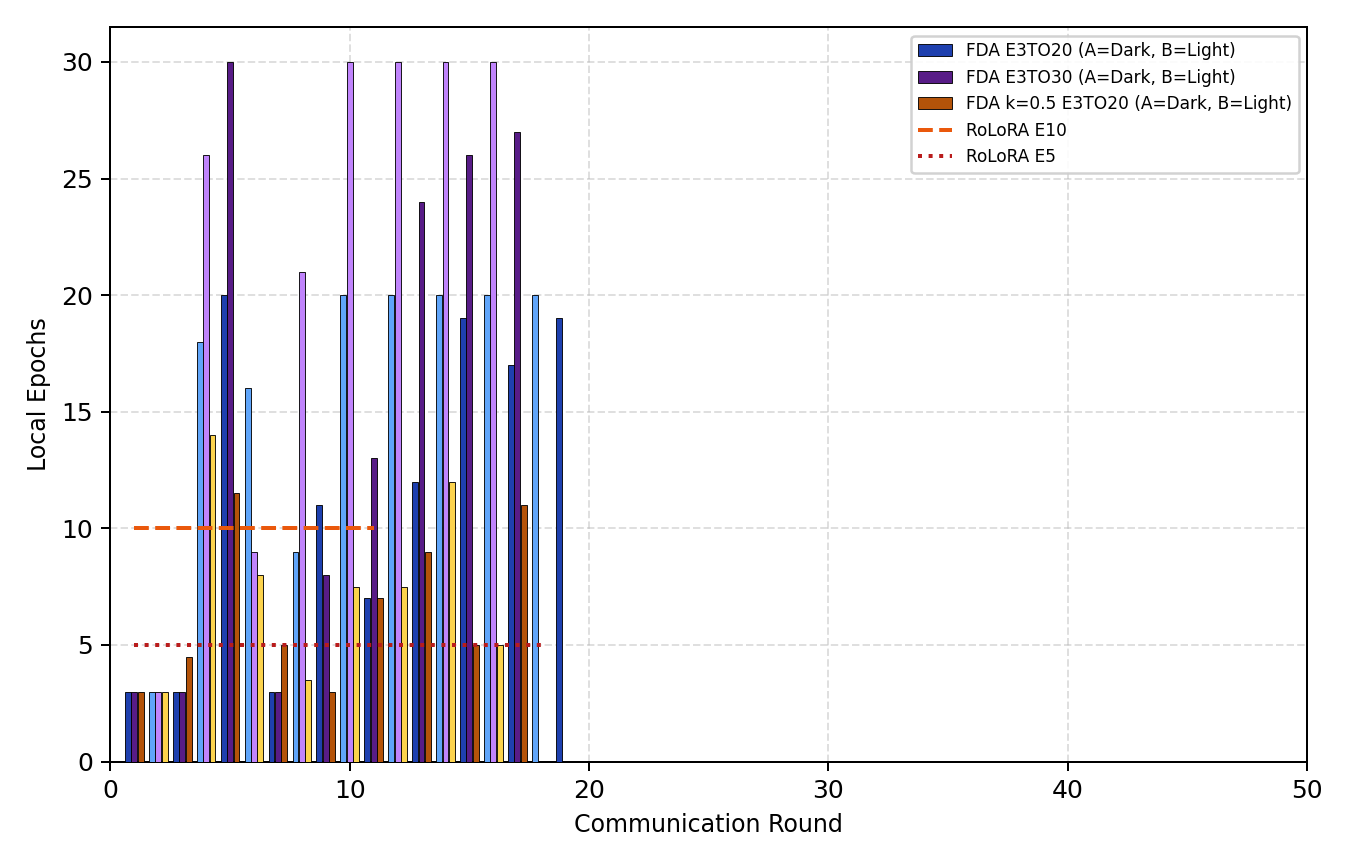
\includegraphics[width=\textwidth,height=4.9cm,keepaspectratio]{figures/telemetry/05_QNLI_C20_R50_LR0.1_2_allocated_epochs.png}
            \vspace{2pt}
            \par{\footnotesize \textbf{(c)} Dynamic Local Epochs ($\bar{e}$)}
        \end{minipage}\hfill
        \begin{minipage}[b]{0.485\textwidth}
            \centering
            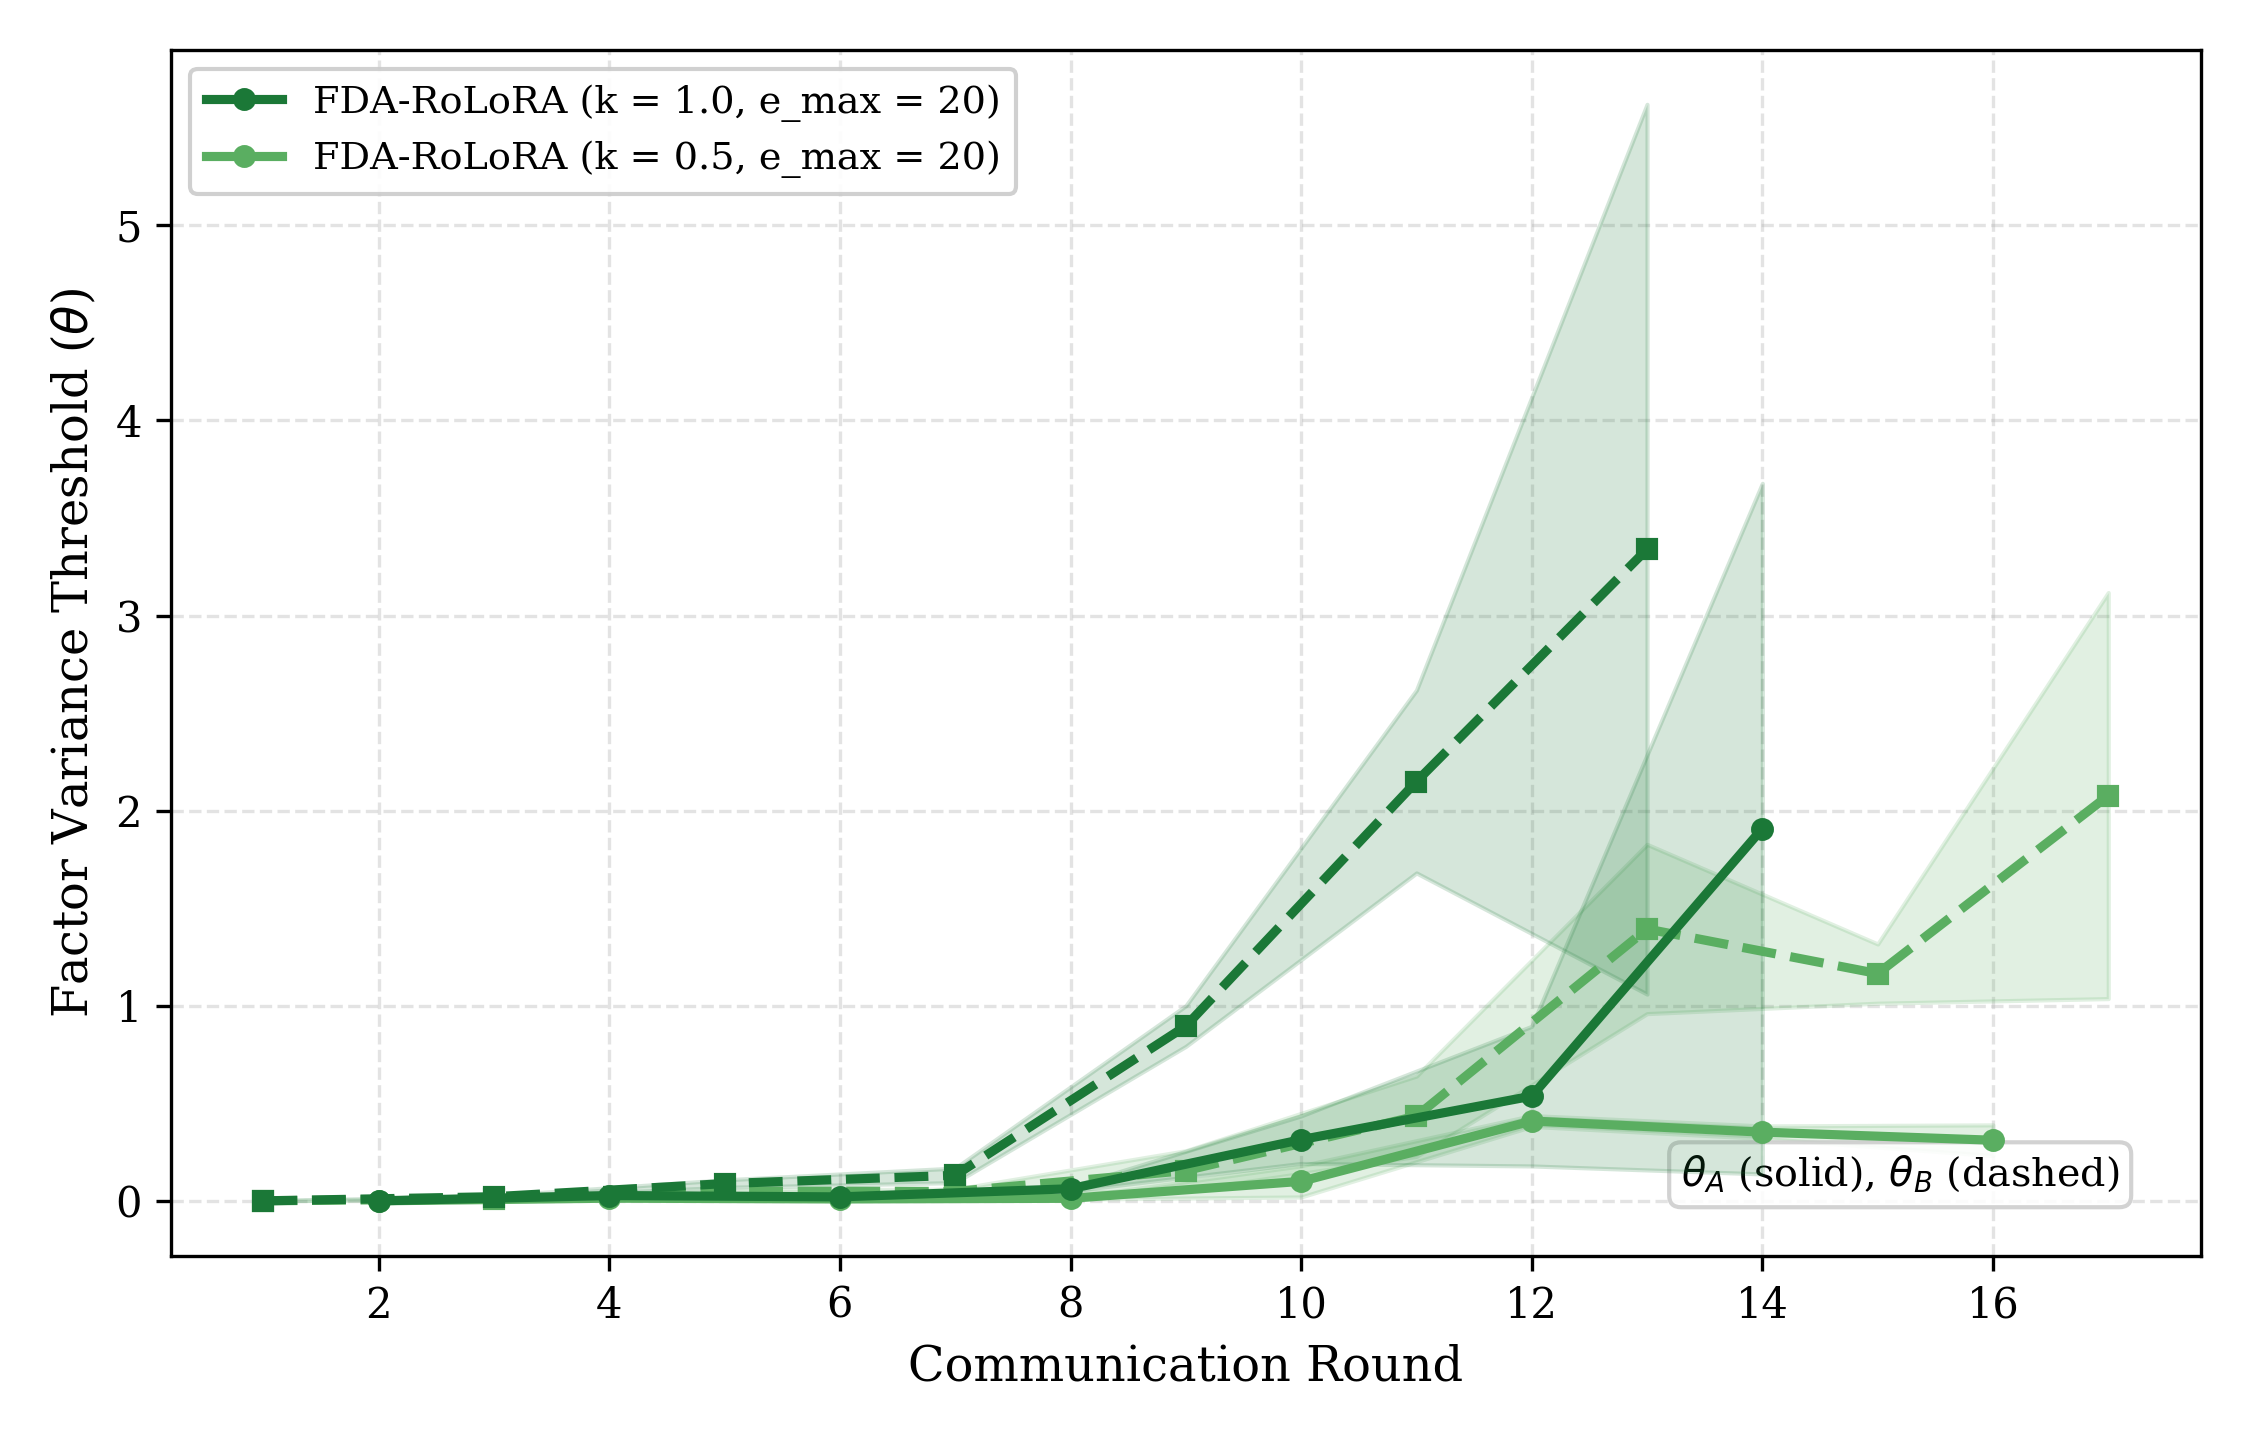
\includegraphics[width=\textwidth,height=4.9cm,keepaspectratio]{figures/telemetry/05_QNLI_C20_R50_LR0.1_5_fda_threshold.png}
            \vspace{2pt}
            \par{\footnotesize \textbf{(d)} Factor Thresholds ($\theta_A, \theta_B$)}
        \end{minipage}

        \vspace{0.6em}
        \begin{minipage}[b]{0.485\textwidth}
            \centering
            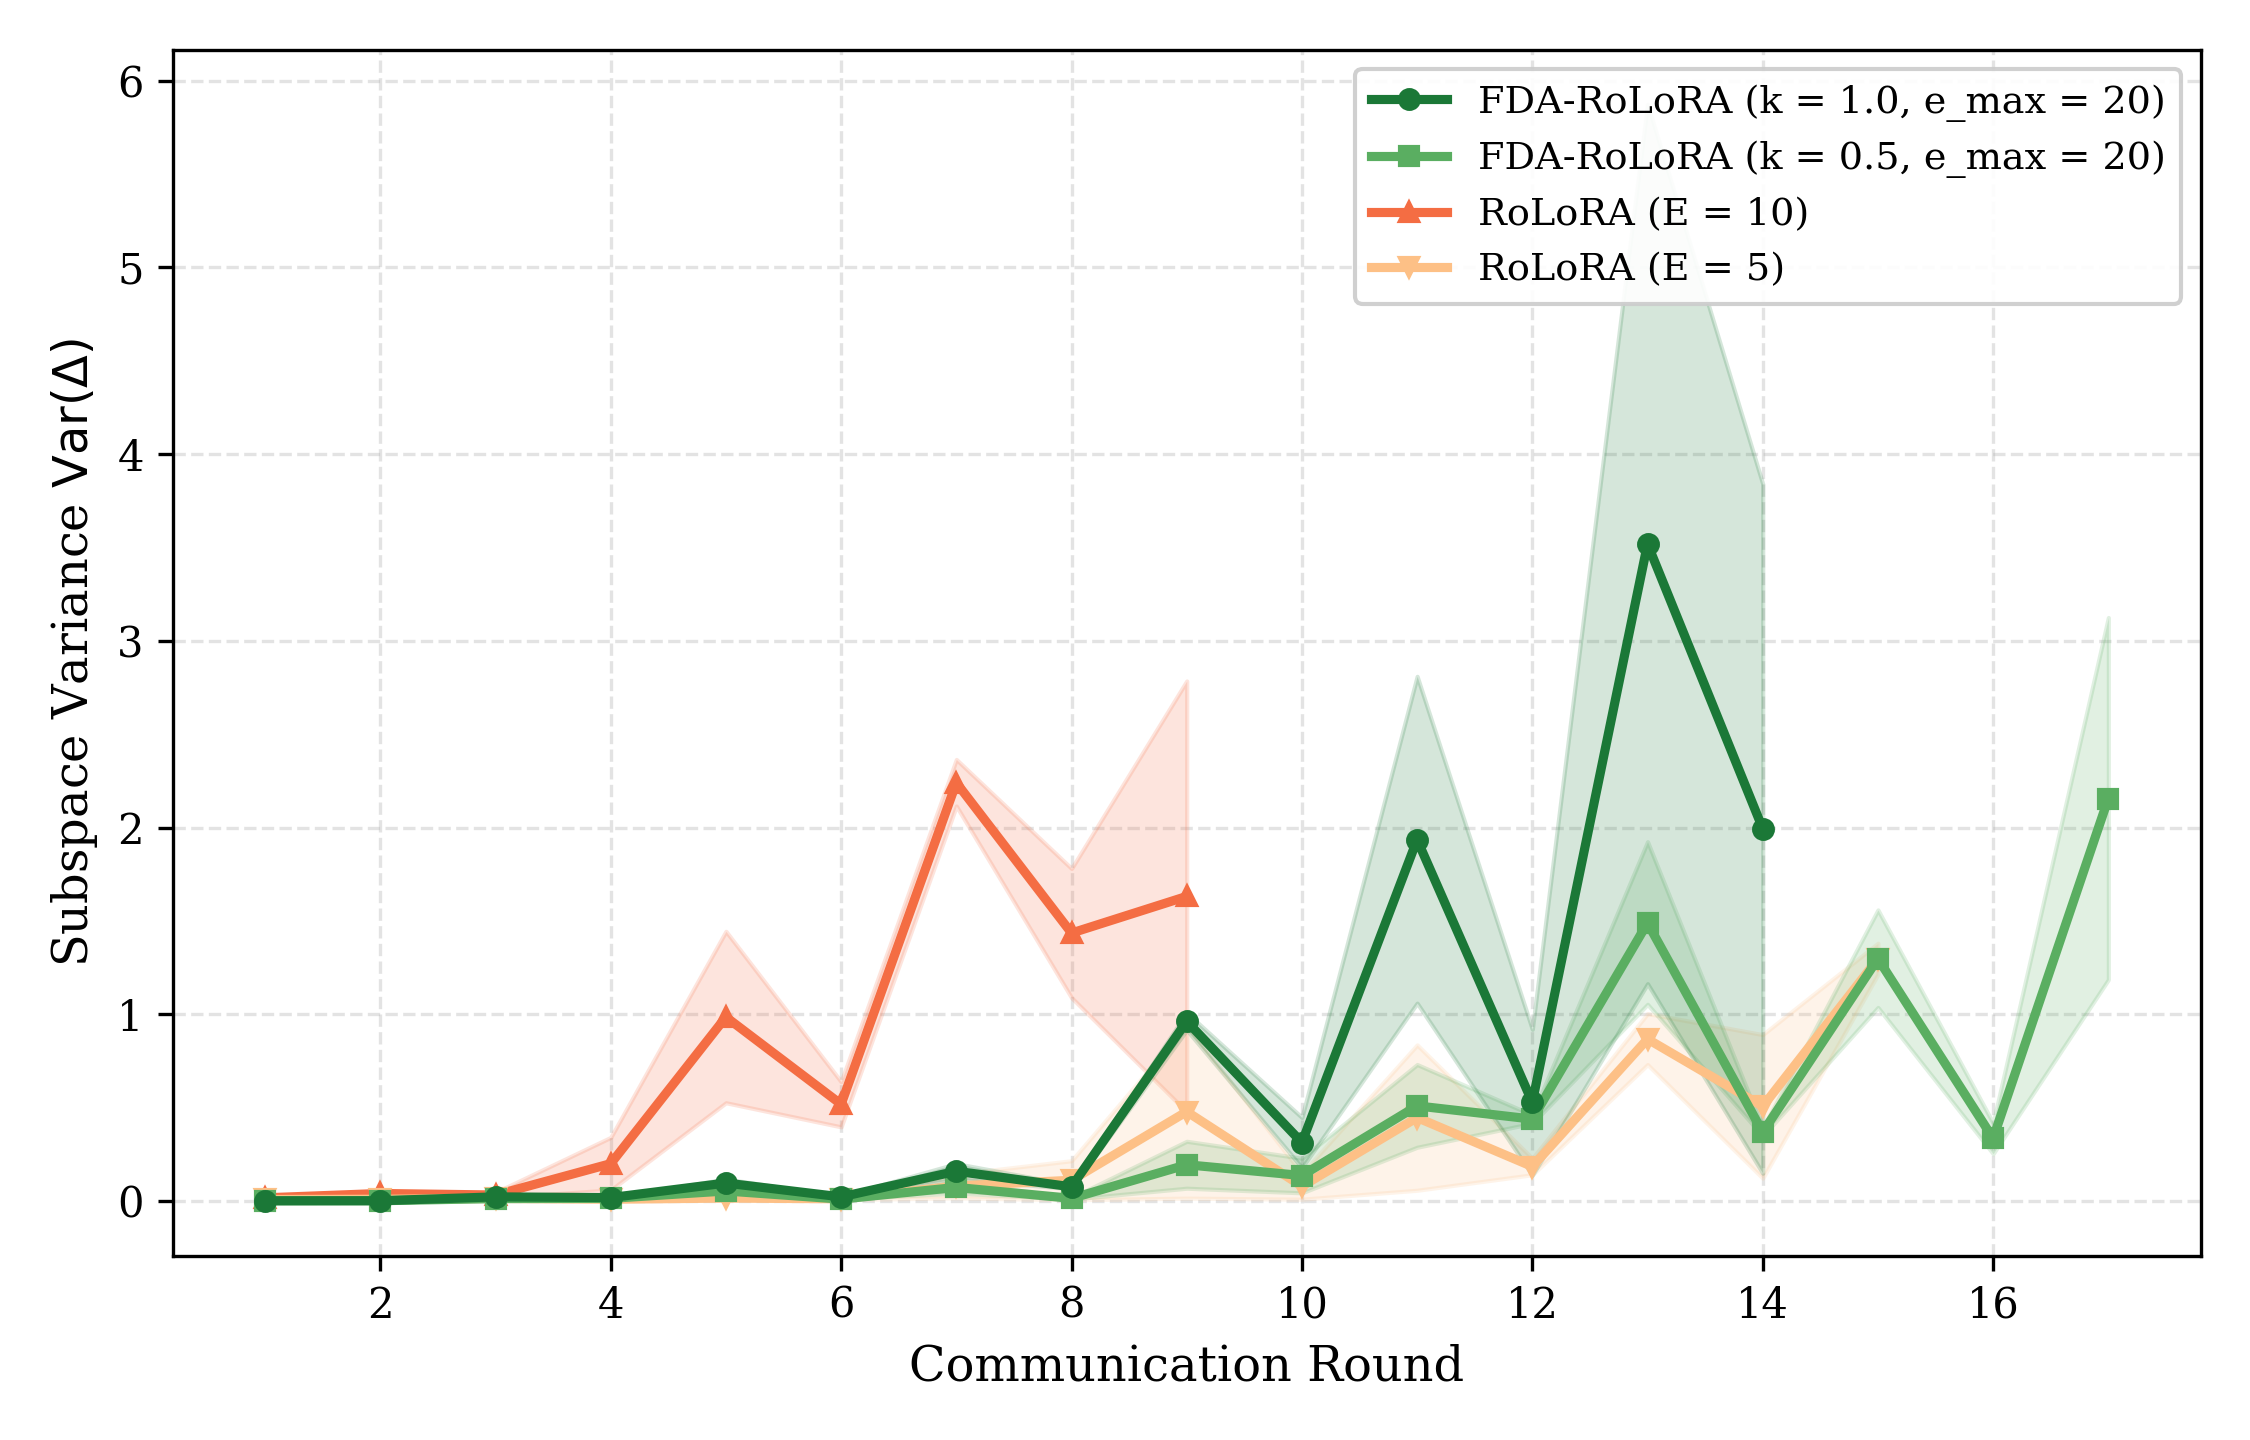
\includegraphics[width=\textwidth,height=4.9cm,keepaspectratio]{figures/telemetry/05_QNLI_C20_R50_LR0.1_3_client_variance.png}
            \vspace{2pt}
            \par{\footnotesize \textbf{(e)} Subspace Coordinate Variance}
        \end{minipage}\hfill
        \begin{minipage}[b]{0.485\textwidth}
            \centering
            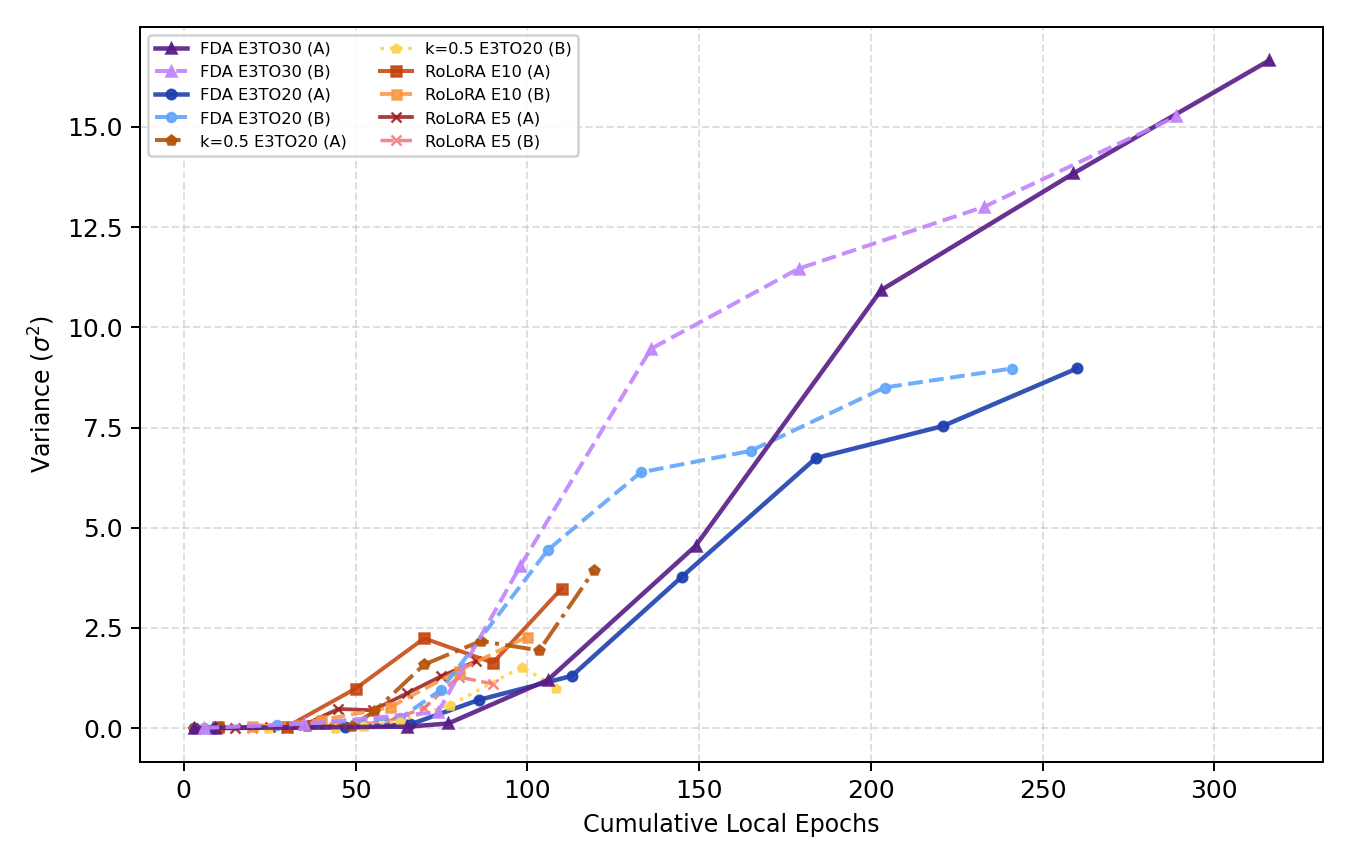
\includegraphics[width=\textwidth,height=4.9cm,keepaspectratio]{figures/telemetry/05_QNLI_C20_R50_LR0.1_6_variance_vs_epoch.png}
            \vspace{2pt}
            \par{\footnotesize \textbf{(f)} Variance vs.\ Cumulative Local Epochs}
        \end{minipage}

        \vspace{0.6em}
        \caption{Multi-panel optimization telemetry on QNLI ($C=20, R_{\max}=50, \eta_c=0.1, \alpha=1000.0$) comparing FDA-RoLoRA against static RoLoRA baselines under homogeneous consensus.}
        \label{fig:telemetry_qnli_c20_iid}
    \end{minipage}%
    }
\end{figure}

\begin{figure}[p]
    \centering
    \makebox[\textwidth][c]{%
    \begin{minipage}{1.06\textwidth}
        \begin{minipage}[b]{0.485\textwidth}
            \centering
            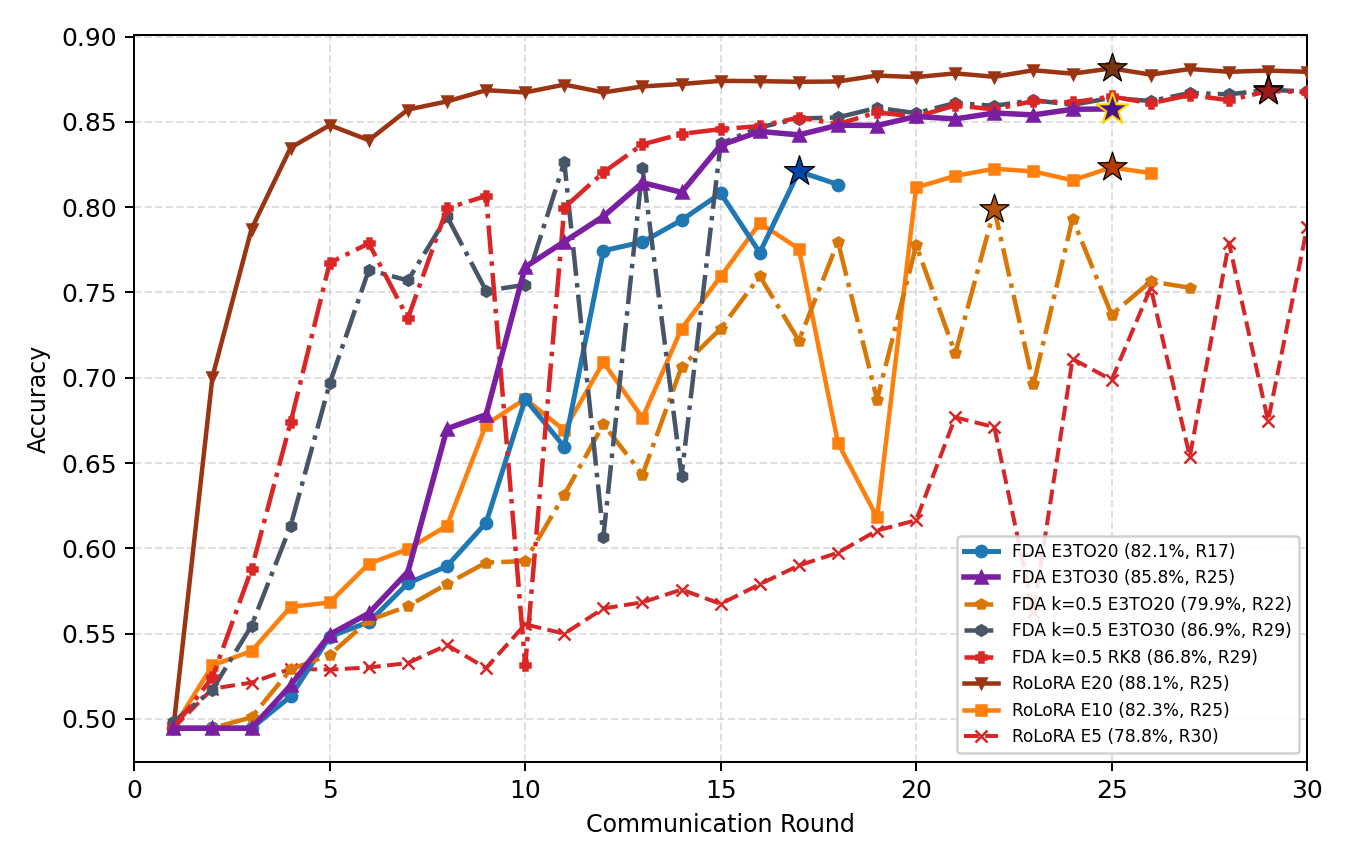
\includegraphics[width=\textwidth,height=4.9cm,keepaspectratio]{figures/telemetry/07_QNLI_C50_R30_LR0.1_1_accuracy.png}
            \vspace{2pt}
            \par{\footnotesize \textbf{(a)} Validation Accuracy}
        \end{minipage}\hfill
        \begin{minipage}[b]{0.485\textwidth}
            \centering
            \includegraphics[width=\textwidth,height=4.9cm,keepaspectratio]{figures/telemetry/07_QNLI_C50_R30_LR0.1_4_accuracy_vs_cost.png}
            \vspace{2pt}
            \par{\footnotesize \textbf{(b)} Accuracy vs. Communication (MB)}
        \end{minipage}

        \vspace{0.6em}
        \begin{minipage}[b]{0.485\textwidth}
            \centering
            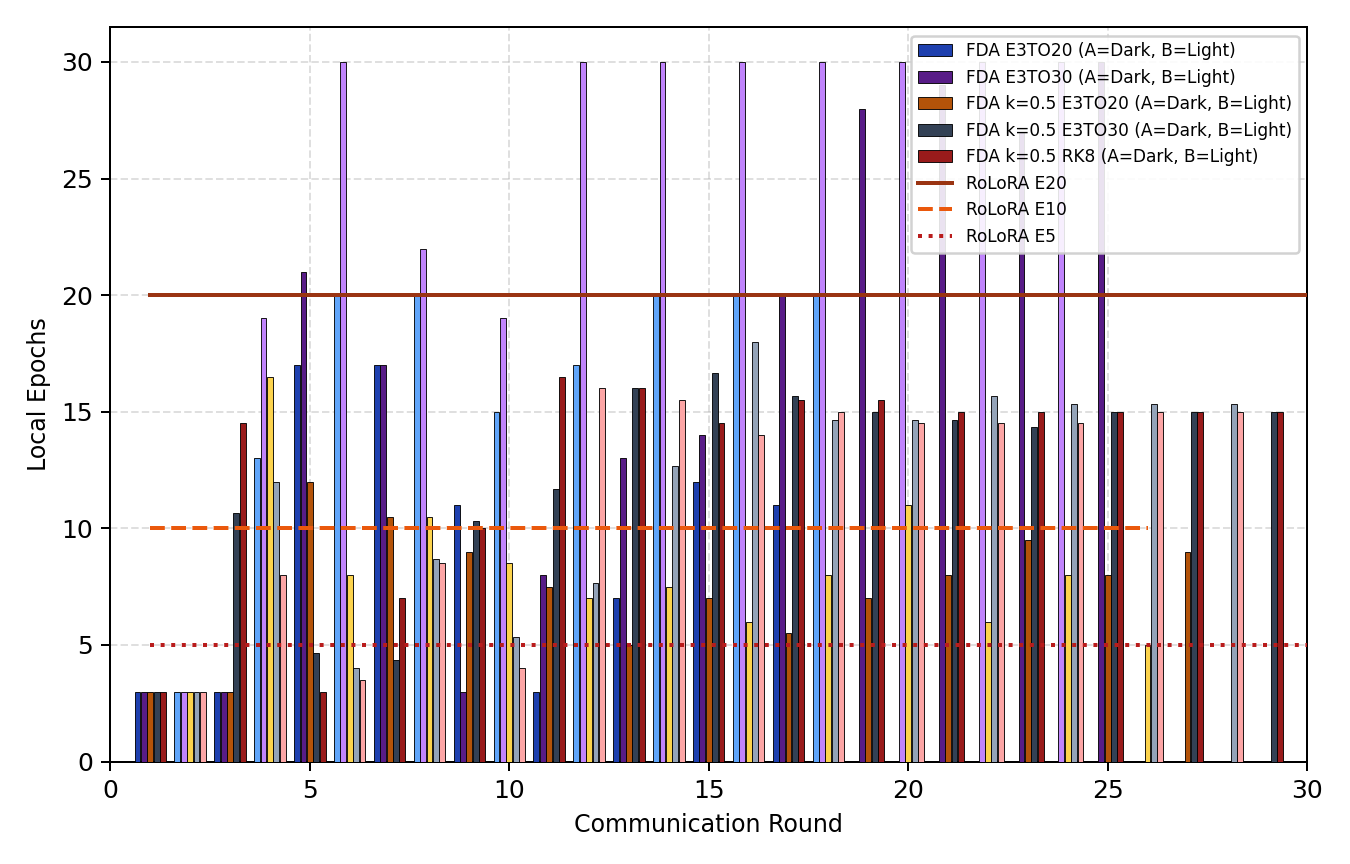
\includegraphics[width=\textwidth,height=4.9cm,keepaspectratio]{figures/telemetry/07_QNLI_C50_R30_LR0.1_2_allocated_epochs.png}
            \vspace{2pt}
            \par{\footnotesize \textbf{(c)} Dynamic Local Epochs ($\bar{e}$)}
        \end{minipage}\hfill
        \begin{minipage}[b]{0.485\textwidth}
            \centering
            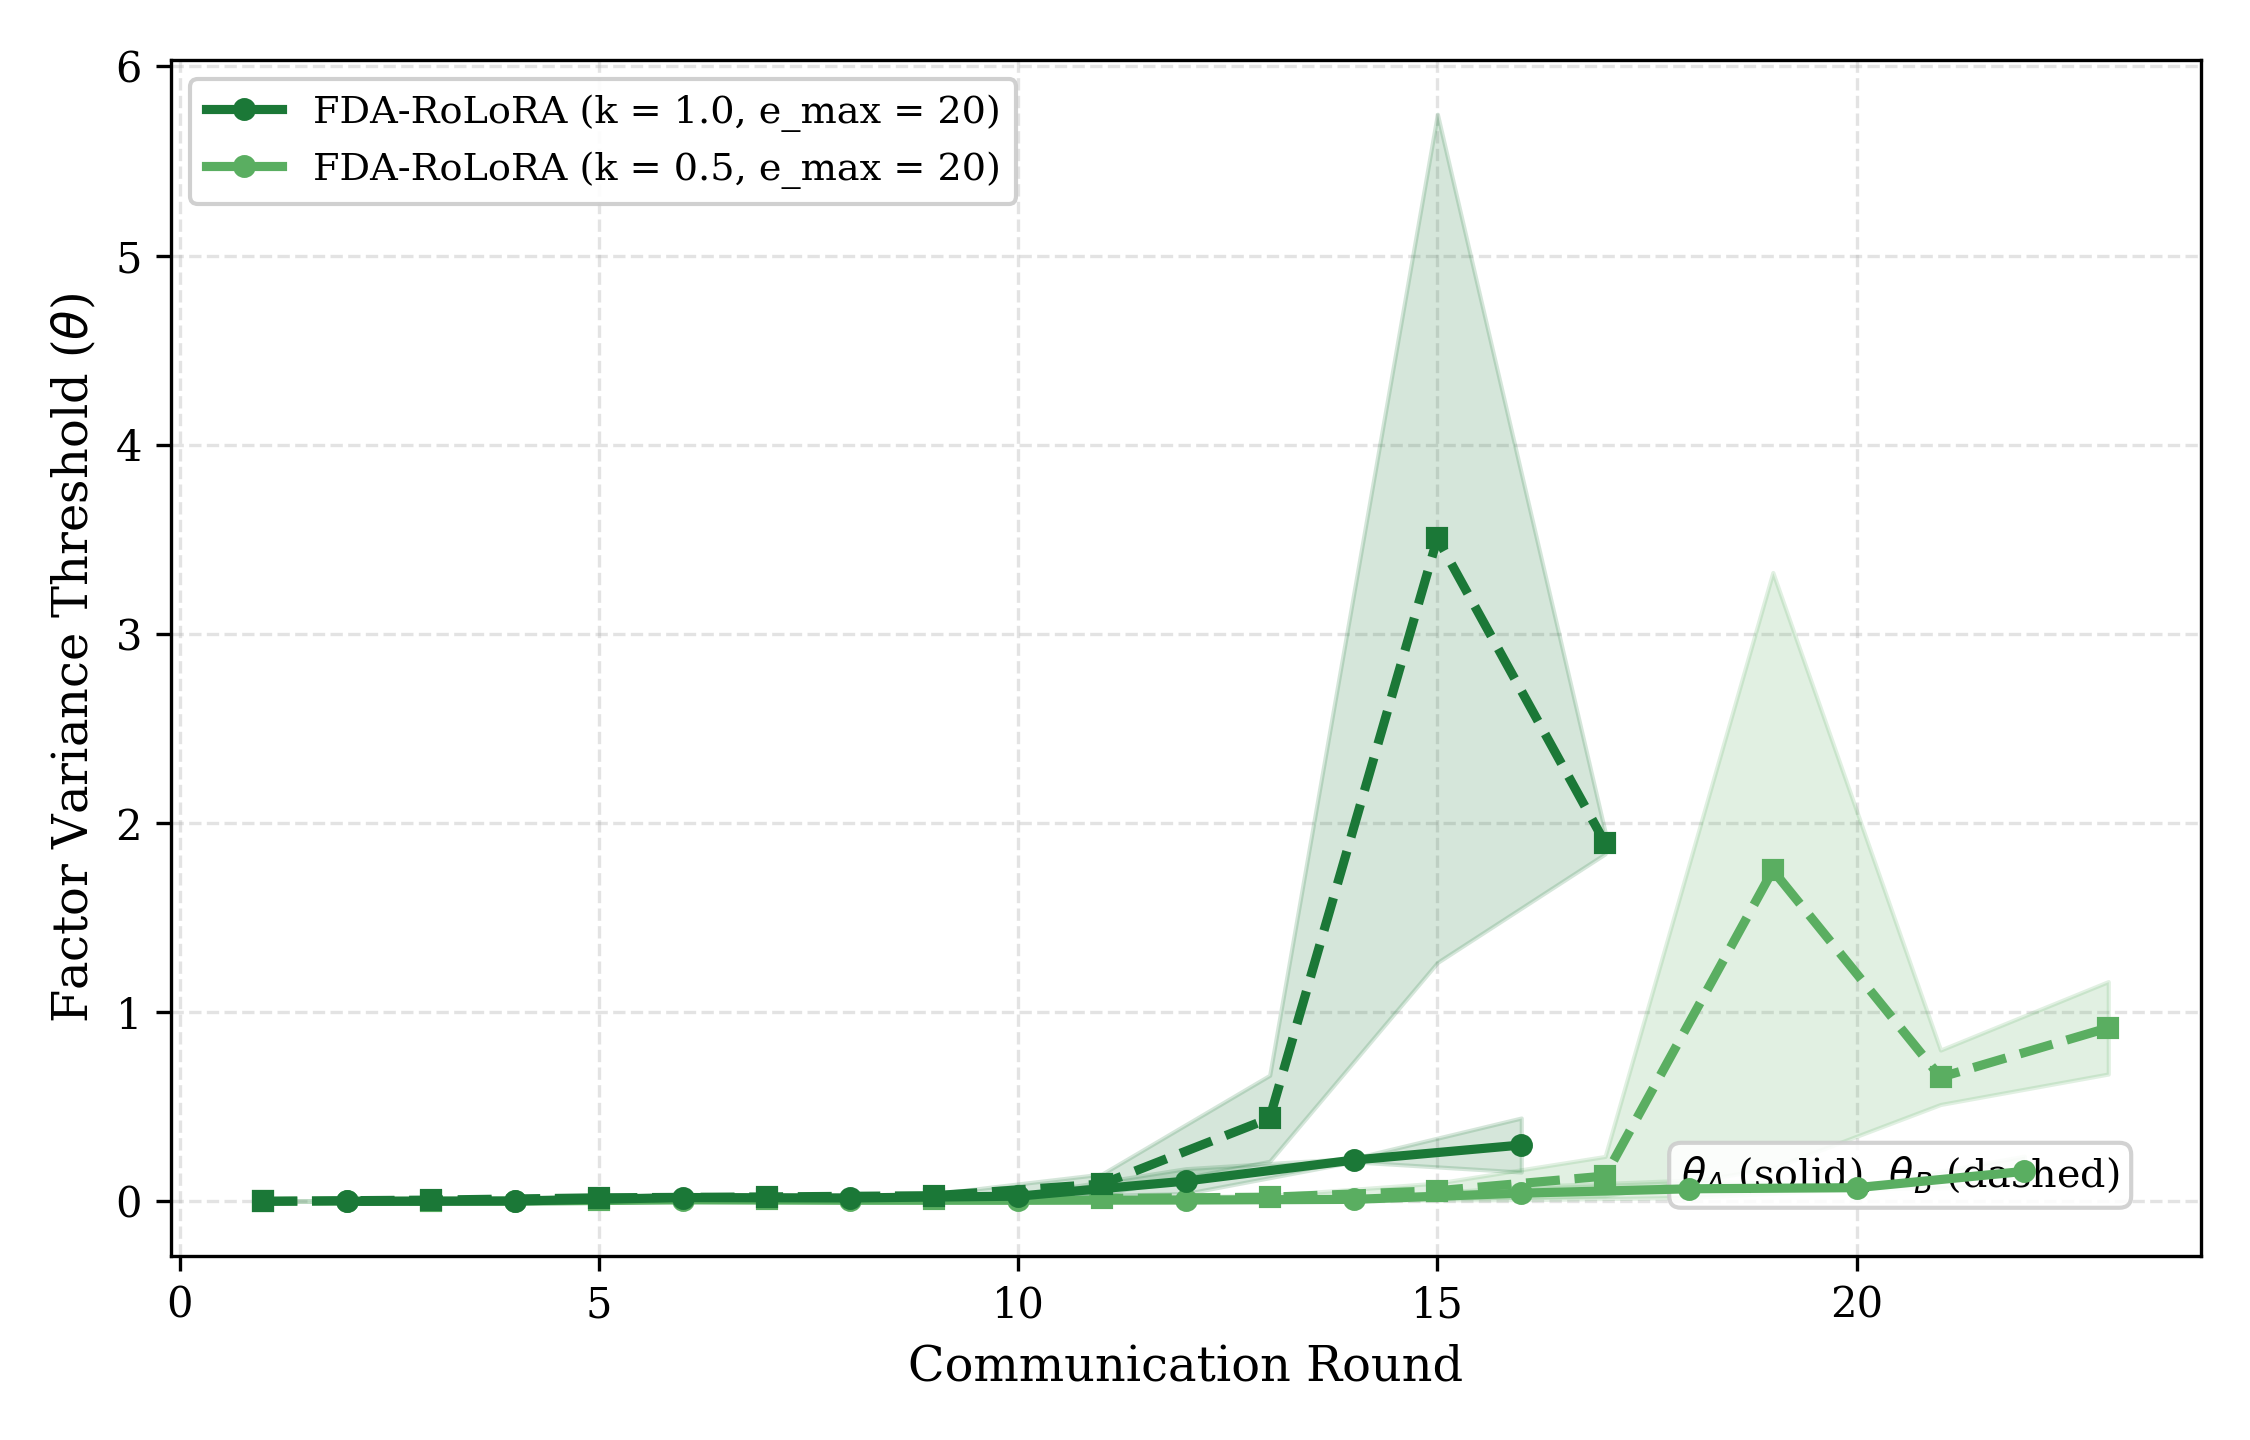
\includegraphics[width=\textwidth,height=4.9cm,keepaspectratio]{figures/telemetry/07_QNLI_C50_R30_LR0.1_5_fda_threshold.png}
            \vspace{2pt}
            \par{\footnotesize \textbf{(d)} Factor Thresholds ($\theta_A, \theta_B$)}
        \end{minipage}

        \vspace{0.6em}
        \begin{minipage}[b]{0.485\textwidth}
            \centering
            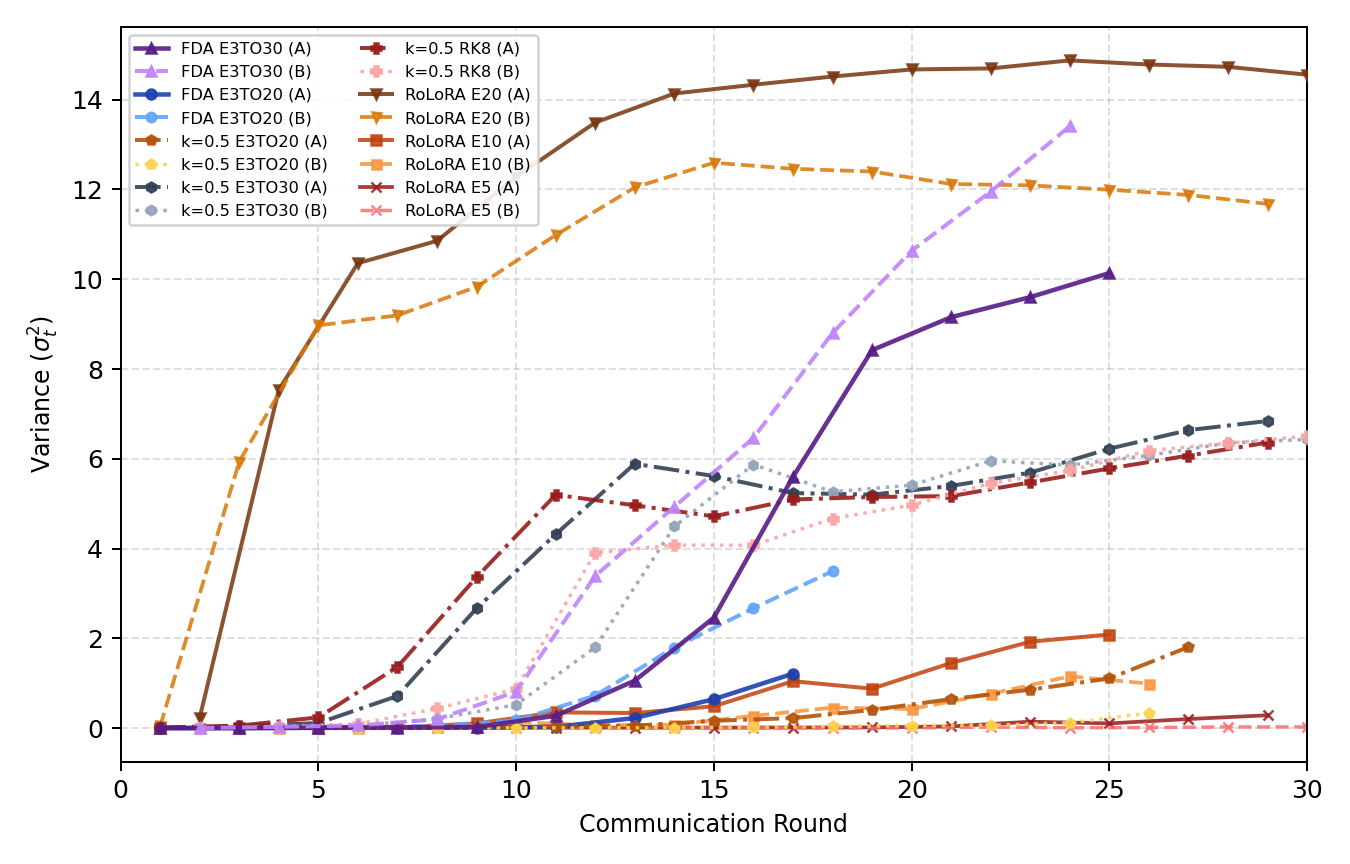
\includegraphics[width=\textwidth,height=4.9cm,keepaspectratio]{figures/telemetry/07_QNLI_C50_R30_LR0.1_3_client_variance.png}
            \vspace{2pt}
            \par{\footnotesize \textbf{(e)} Subspace Coordinate Variance}
        \end{minipage}\hfill
        \begin{minipage}[b]{0.485\textwidth}
            \centering
            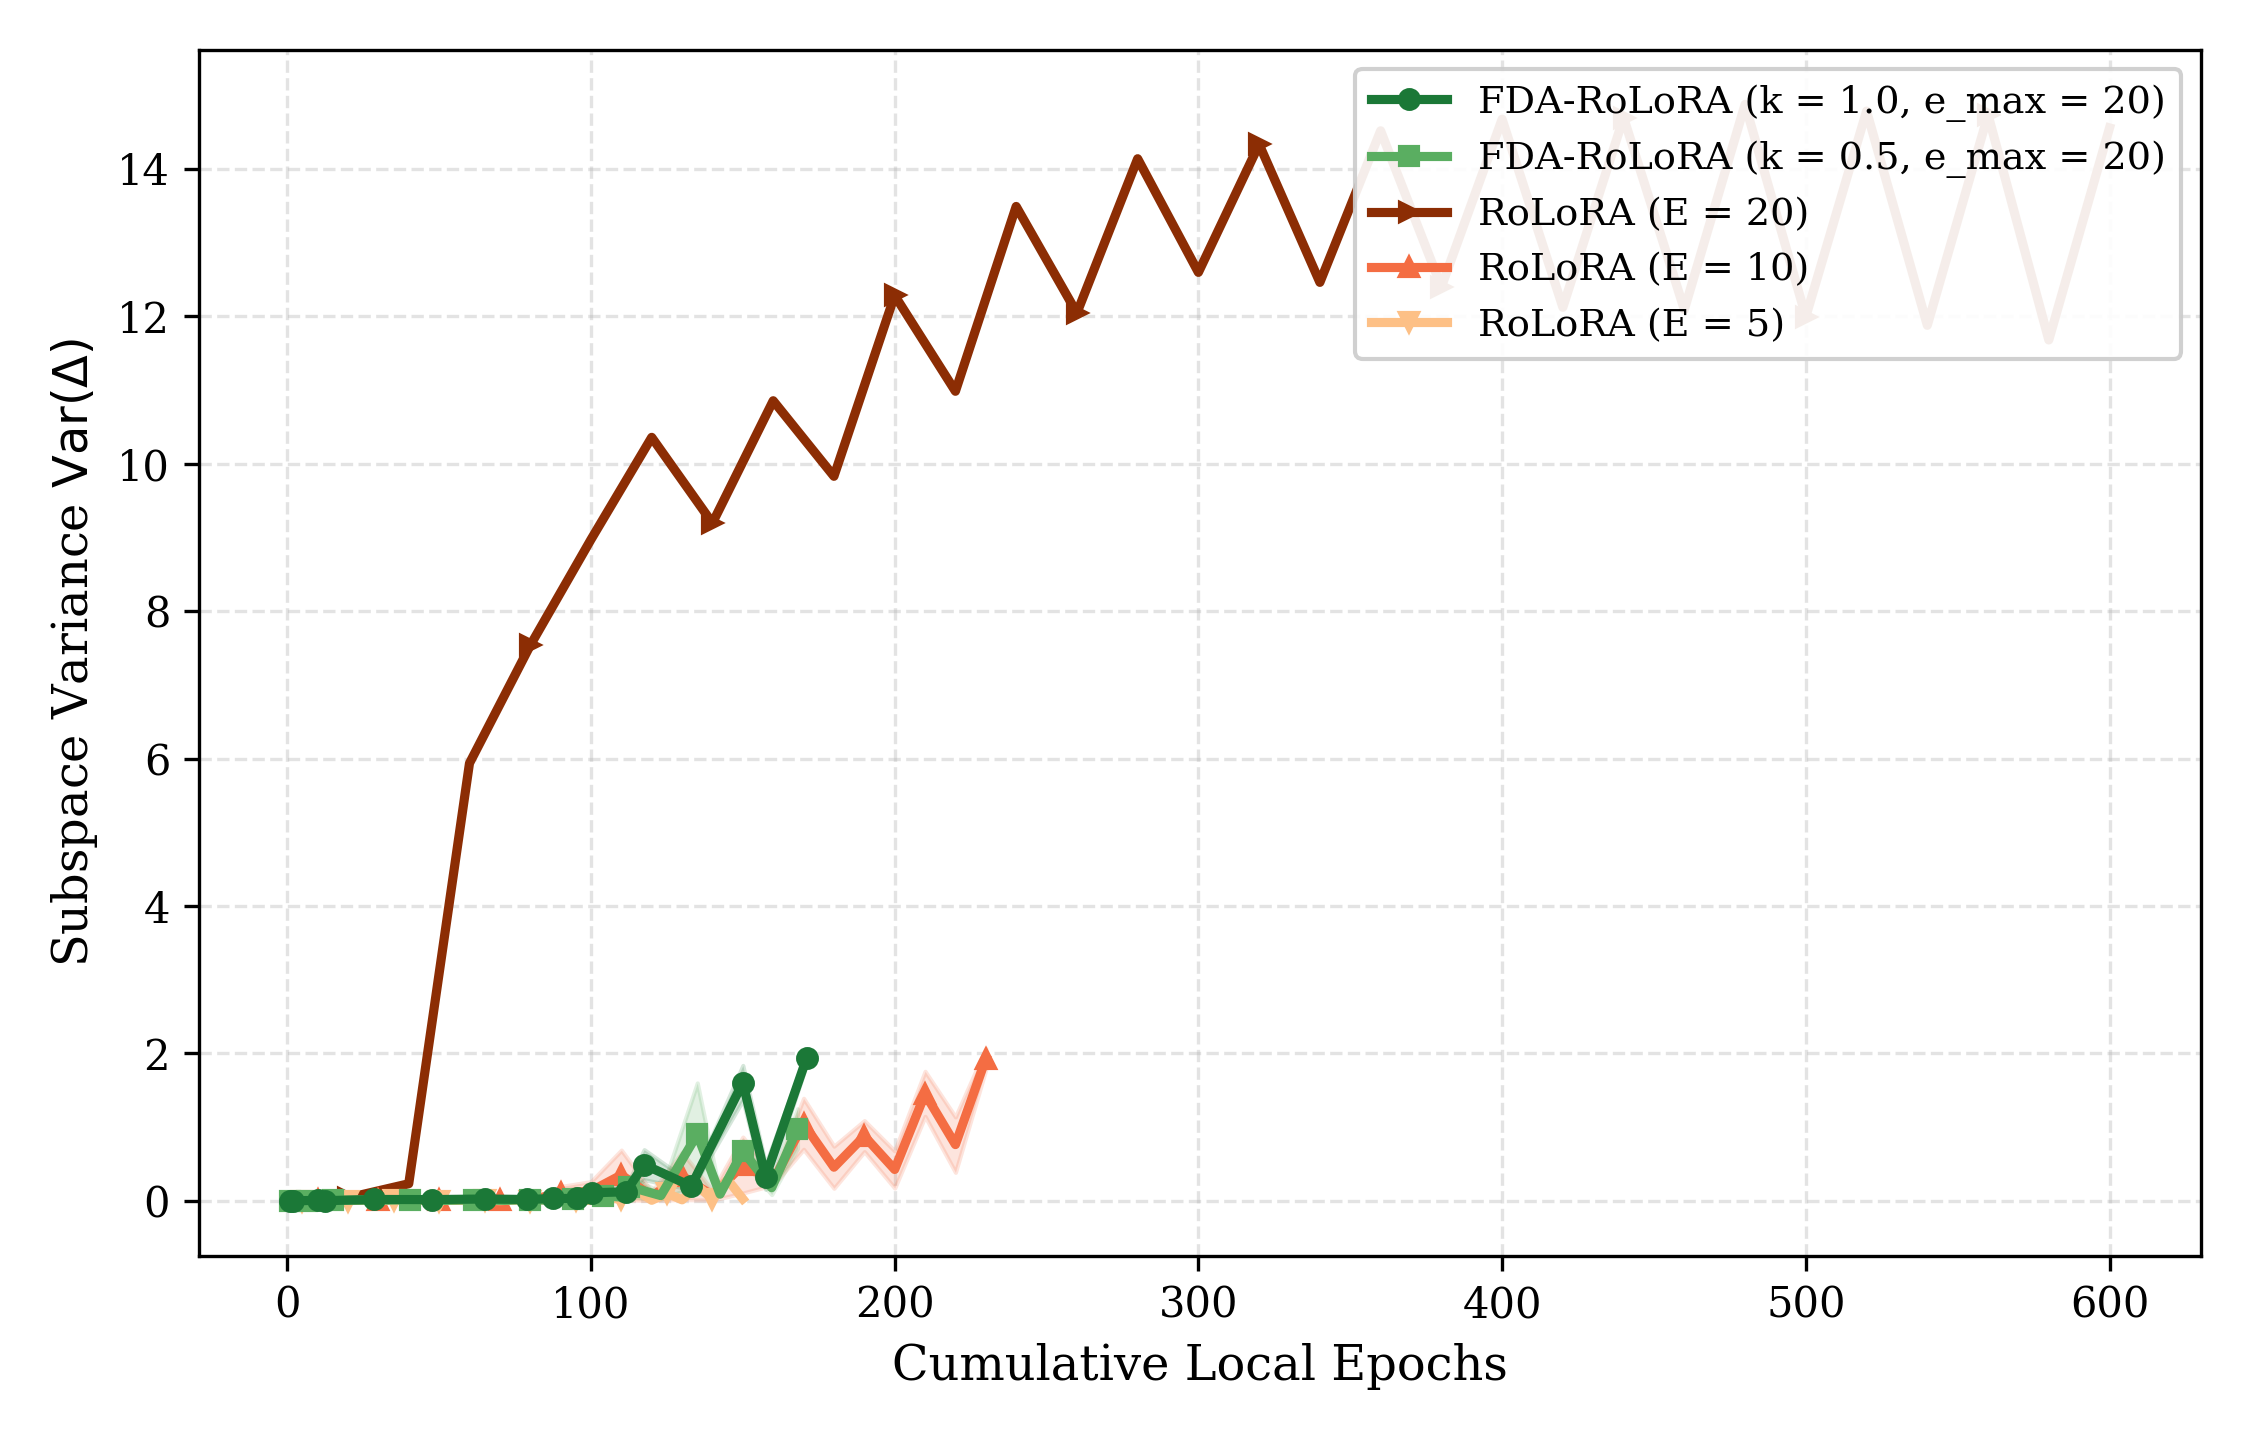
\includegraphics[width=\textwidth,height=4.9cm,keepaspectratio]{figures/telemetry/07_QNLI_C50_R30_LR0.1_6_variance_vs_epoch.png}
            \vspace{2pt}
            \par{\footnotesize \textbf{(f)} Variance vs.\ Cumulative Local Epochs}
        \end{minipage}

        \vspace{0.6em}
        \caption{Multi-panel optimization telemetry on QNLI ($C=50, R_{\max}=30, \eta_c=0.1, \alpha=1000.0$) under expanded cohort scale $C=50$.}
        \label{fig:telemetry_qnli_c50_iid}
    \end{minipage}%
    }
\end{figure}

\paragraph{QQP:}
Semantic paraphrase detection demonstrates the primary communication compression benefits of dynamic averaging. Figures~\ref{fig:telemetry_qqp_c20_iid} and \ref{fig:telemetry_qqp_c50_iid} illustrate QQP telemetry across all six metrics. On $C=20$ (Figure~\ref{fig:telemetry_qqp_c20_iid}), FDA-RoLoRA ($k=1.0$) attains $\mathbf{78.57\%}$ peak validation accuracy (Panel a), outperforming RoLoRA $E=10$ ($75.47\%$) by $\mathbf{+3.10\%}$ while shifting the cost Pareto curve leftward (Panel b). Realized local epochs (Panel c) average $\bar{e} = 10.69$ under $k=1.0$ (and $\bar{e} = 6.50$ under $k=0.5$). Factor threshold tracks (Panel d) adapt smoothly without volatility, while subspace coordinate variance (Panel e) is strictly bounded ($\bar{\nu} = 1.577$).

On $C=50$ (Figure~\ref{fig:telemetry_qqp_c50_iid}), static RoLoRA baselines require the full budget of $30.0$ rounds ($351.6\,\text{MB}$) without reaching early stopping. In contrast, FDA-RoLoRA ($k=1.0$) triggers early stopping after $14.0$ rounds ($164.1\,\text{MB}$) at a lower accuracy plateau (final $72.65\%$, peak $73.63\%$) than RoLoRA $E=10$ (final $75.43\%$, peak $78.79\%$). At the same round (round 14), RoLoRA $E=10$ had already reached $75.27\%$ and $75.90\%$ in the two seeds, and it matched FDA-RoLoRA's final accuracy by round 6--7. The earlier stop therefore reflects an earlier plateau, not a communication saving at equal accuracy. Guided by suppressed drift variance ($\bar{\nu} = 0.220$, Panel e), the controller safely executes $\bar{e} = 9.14$ epochs per round before synchronization.
\begin{figure}[p]
    \centering
    \makebox[\textwidth][c]{%
    \begin{minipage}{1.06\textwidth}
        \begin{minipage}[b]{0.485\textwidth}
            \centering
            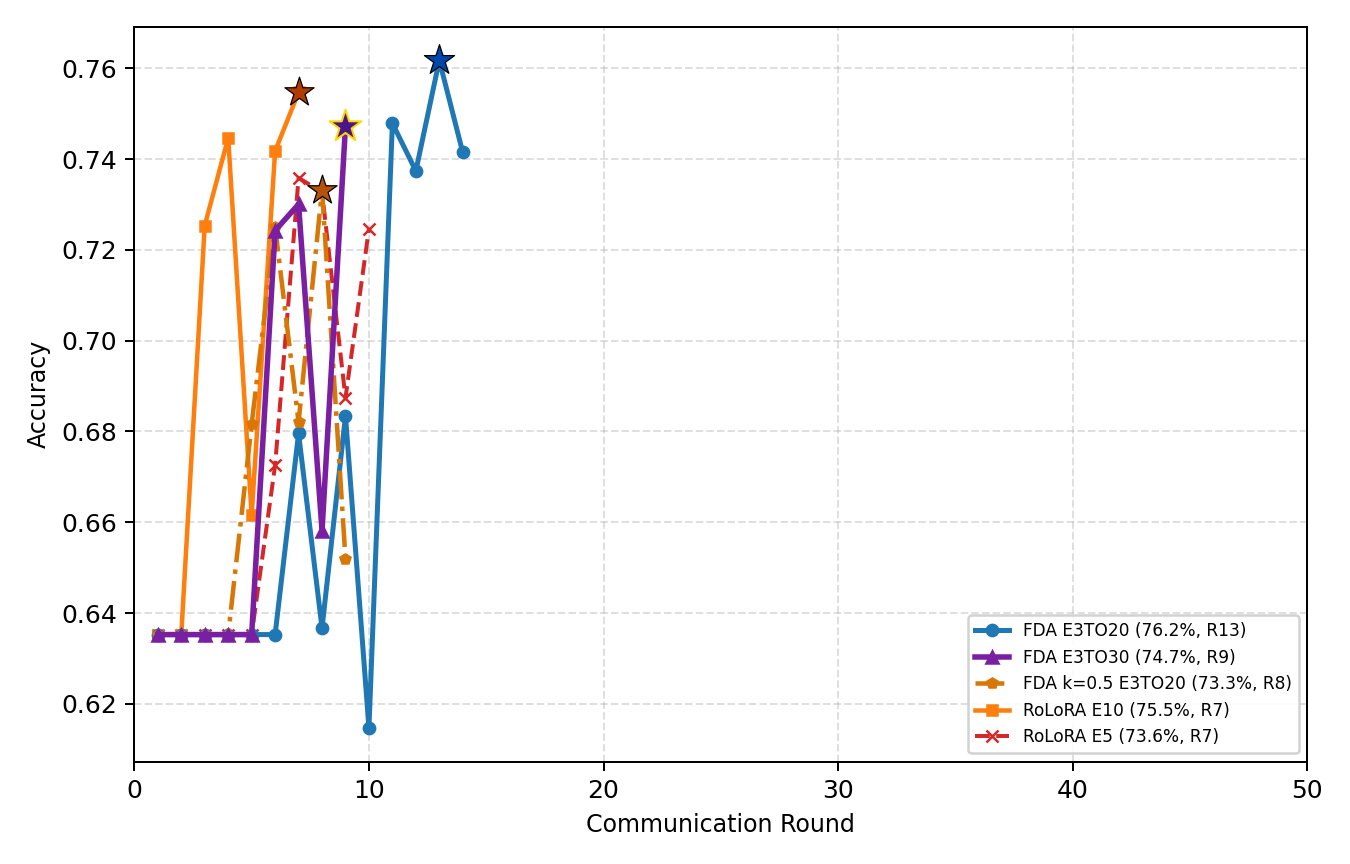
\includegraphics[width=\textwidth,height=4.9cm,keepaspectratio]{figures/telemetry/09_QQP_C20_R50_LR0.1_1_accuracy.png}
            \vspace{2pt}
            \par{\footnotesize \textbf{(a)} Validation Accuracy}
        \end{minipage}\hfill
        \begin{minipage}[b]{0.485\textwidth}
            \centering
            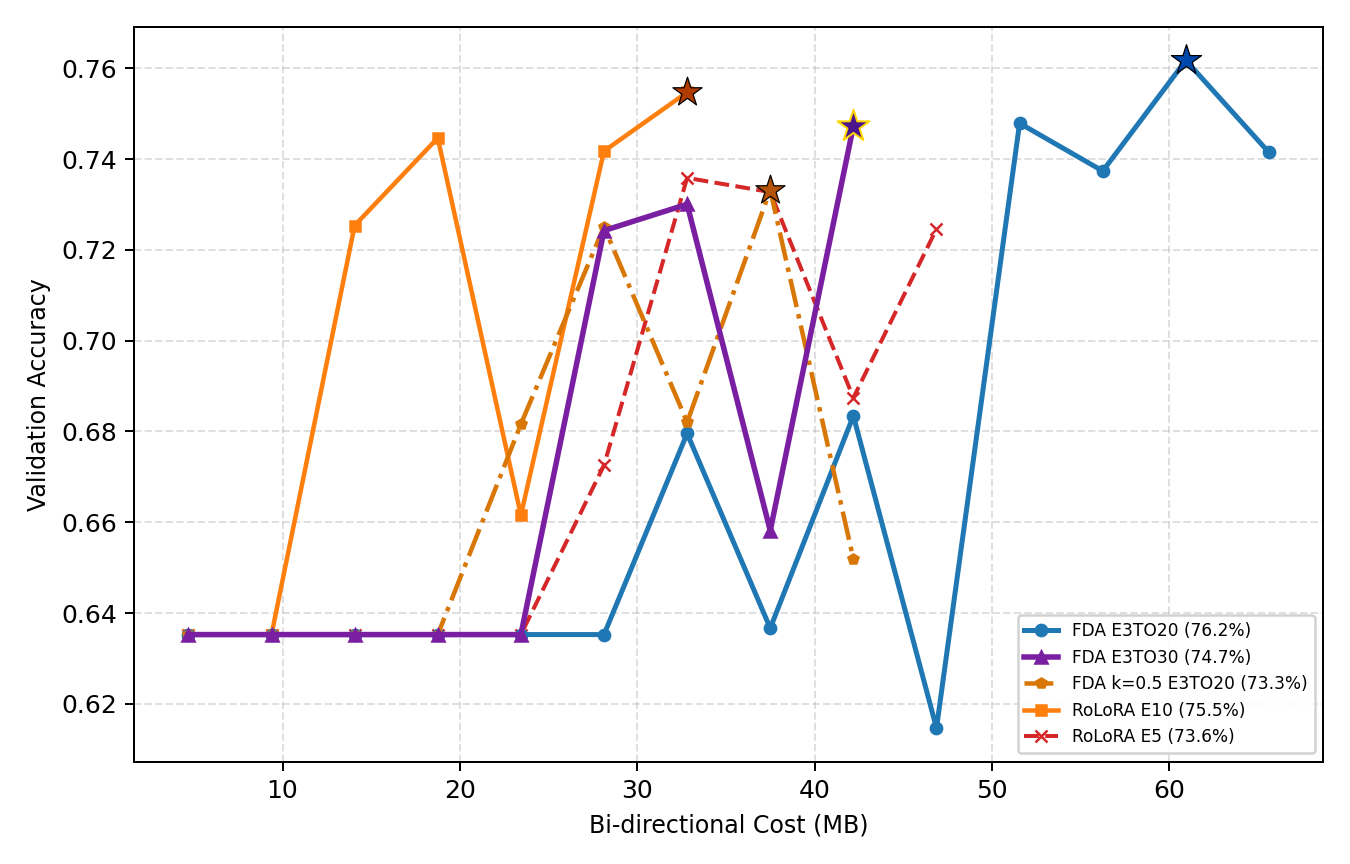
\includegraphics[width=\textwidth,height=4.9cm,keepaspectratio]{figures/telemetry/09_QQP_C20_R50_LR0.1_4_accuracy_vs_cost.png}
            \vspace{2pt}
            \par{\footnotesize \textbf{(b)} Accuracy vs. Communication (MB)}
        \end{minipage}

        \vspace{0.6em}
        \begin{minipage}[b]{0.485\textwidth}
            \centering
            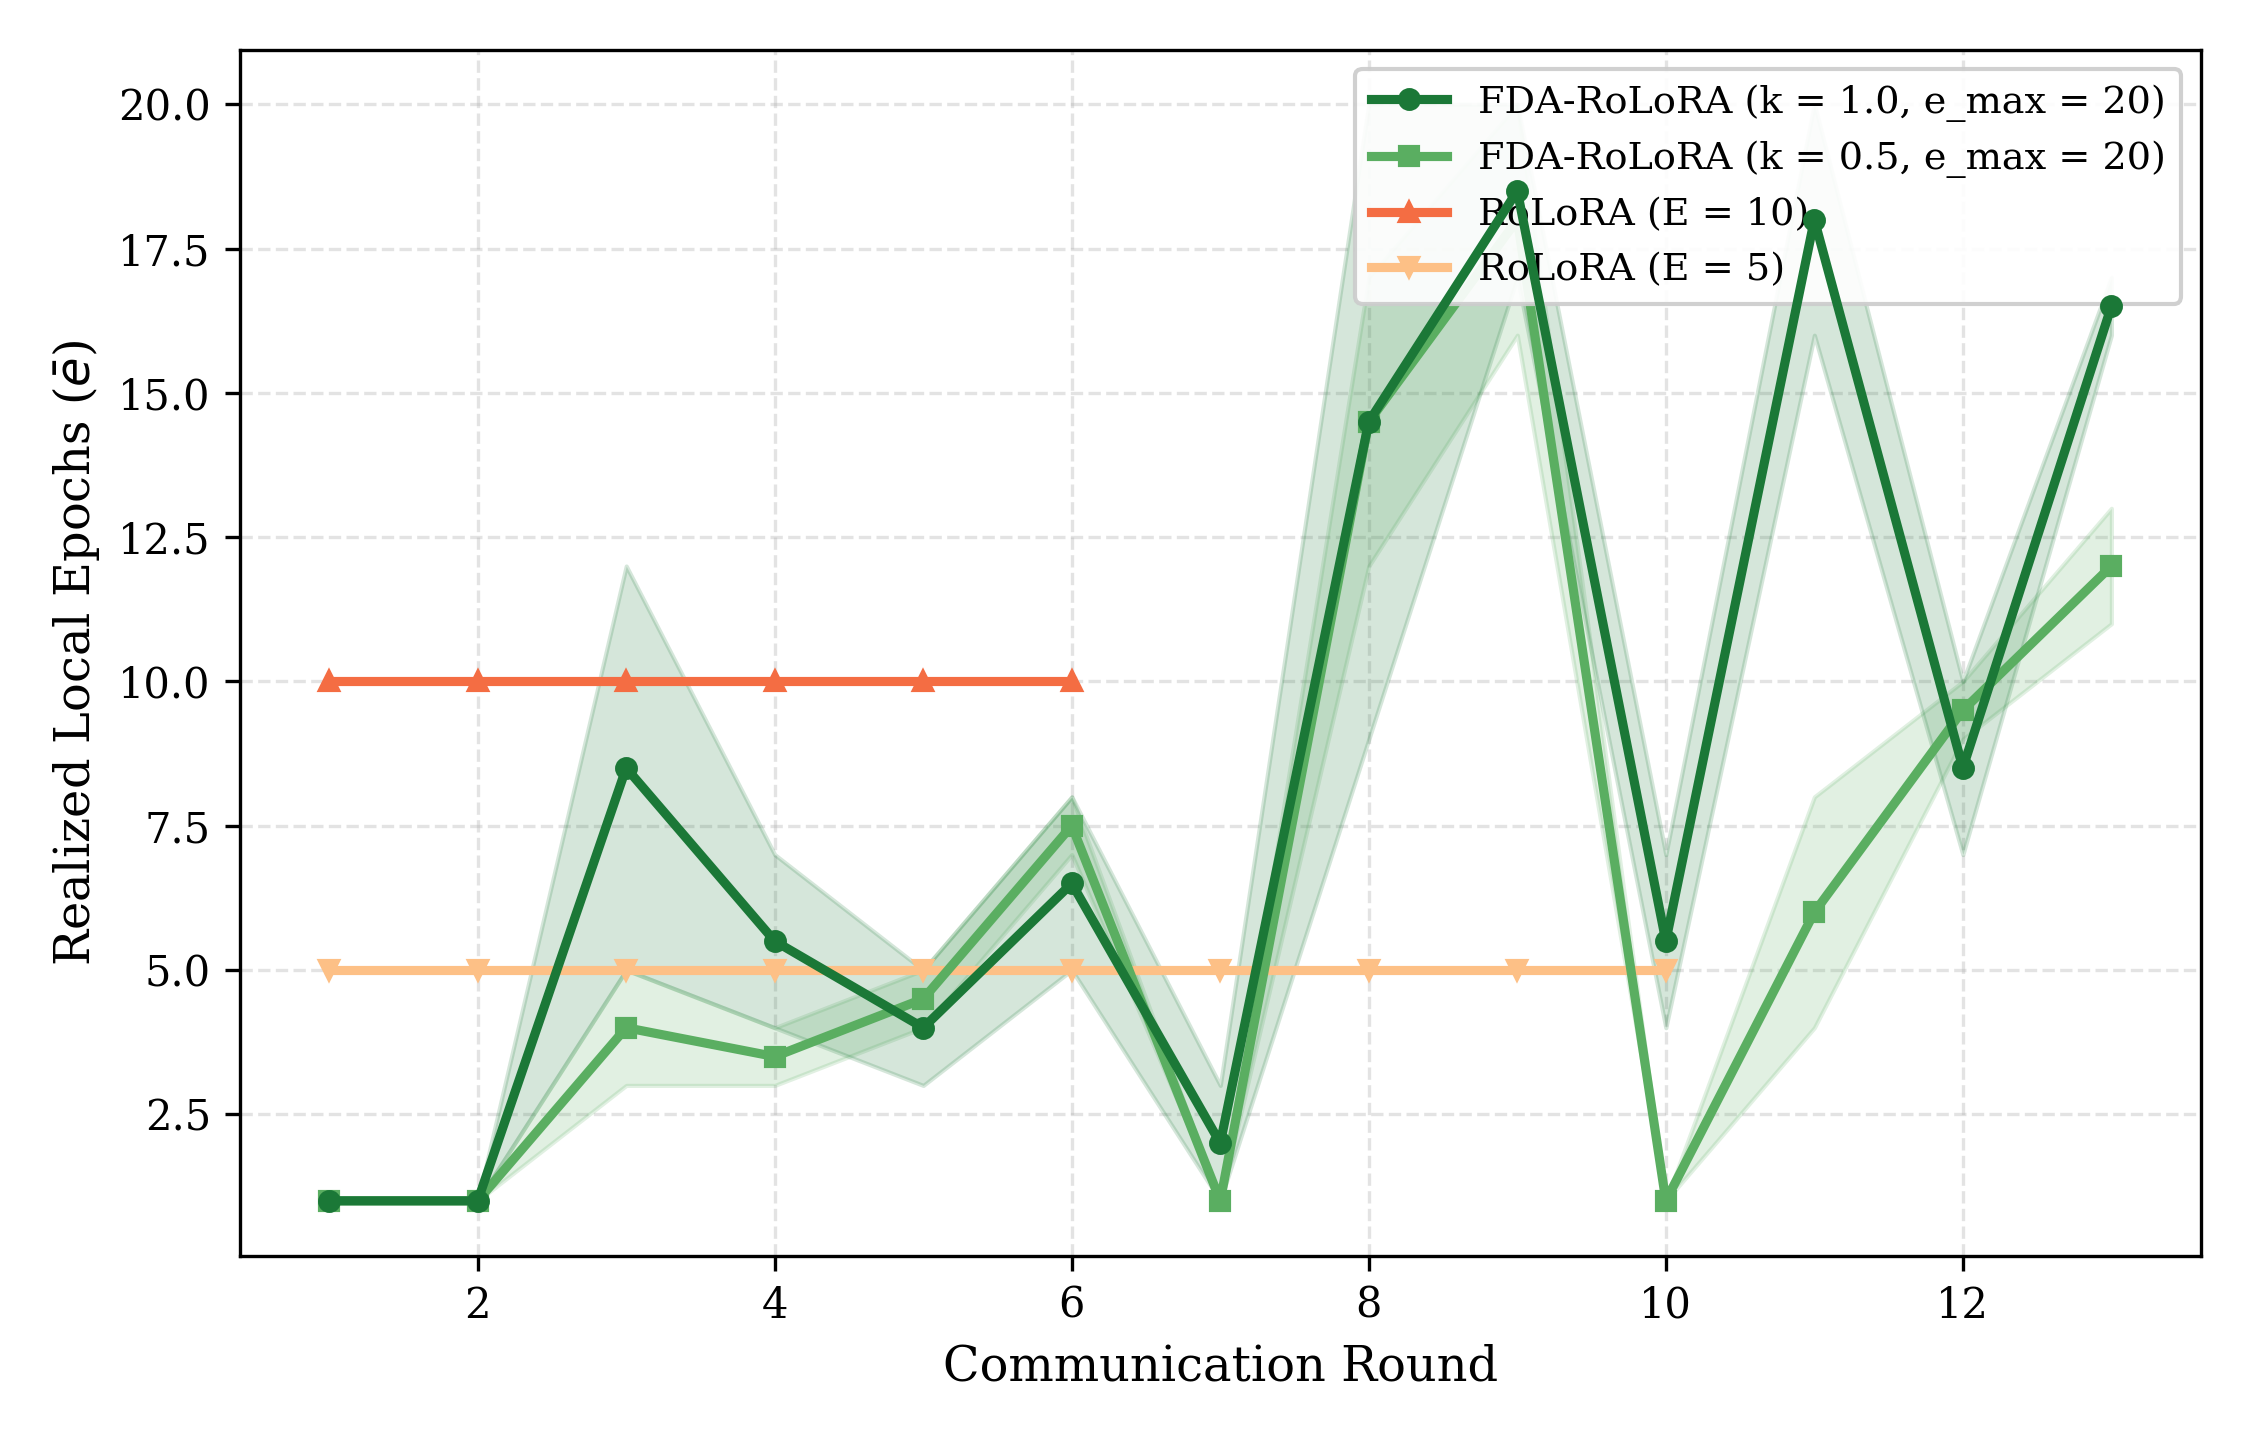
\includegraphics[width=\textwidth,height=4.9cm,keepaspectratio]{figures/telemetry/09_QQP_C20_R50_LR0.1_2_allocated_epochs.png}
            \vspace{2pt}
            \par{\footnotesize \textbf{(c)} Dynamic Local Epochs ($\bar{e}$)}
        \end{minipage}\hfill
        \begin{minipage}[b]{0.485\textwidth}
            \centering
            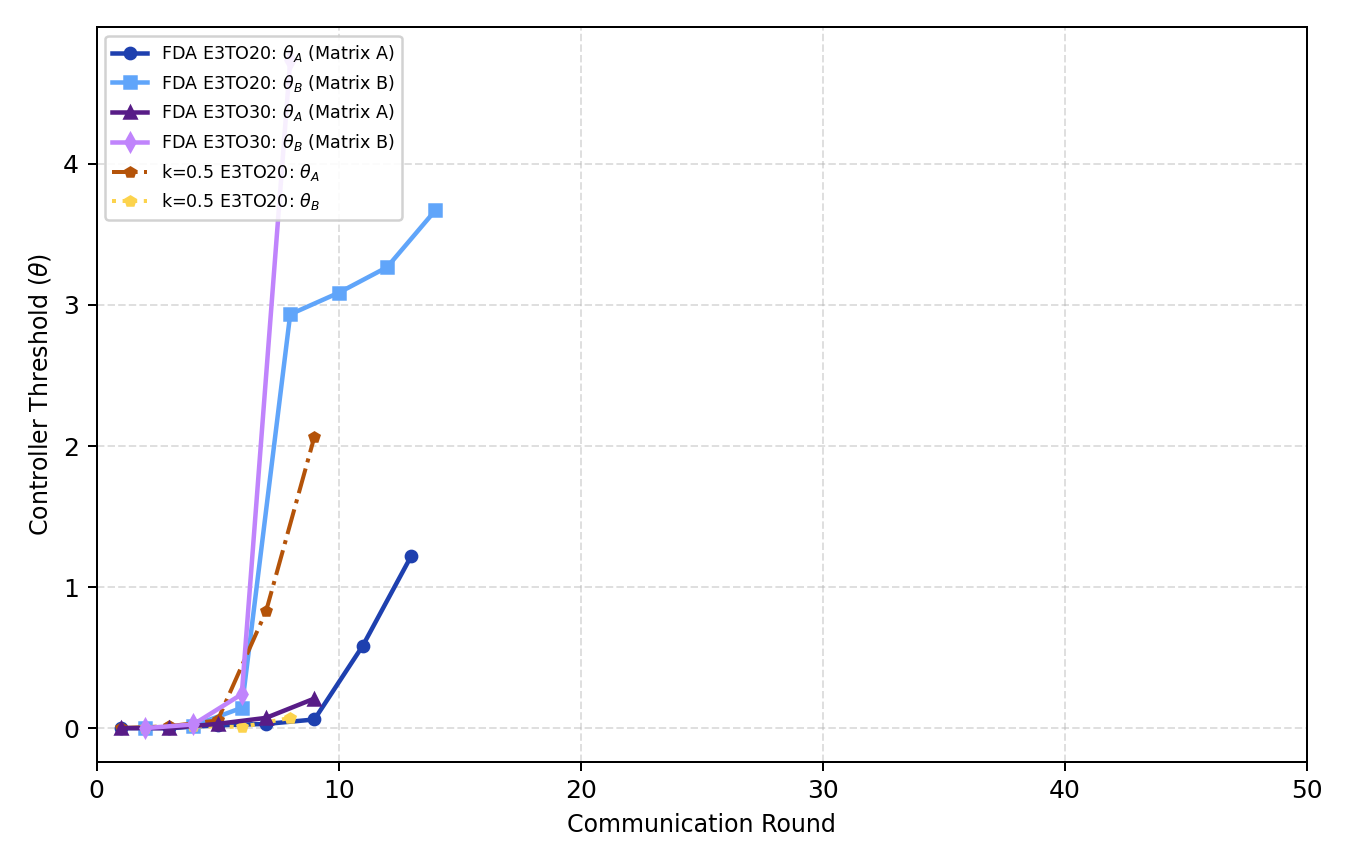
\includegraphics[width=\textwidth,height=4.9cm,keepaspectratio]{figures/telemetry/09_QQP_C20_R50_LR0.1_5_fda_threshold.png}
            \vspace{2pt}
            \par{\footnotesize \textbf{(d)} Factor Thresholds ($\theta_A, \theta_B$)}
        \end{minipage}

        \vspace{0.6em}
        \begin{minipage}[b]{0.485\textwidth}
            \centering
            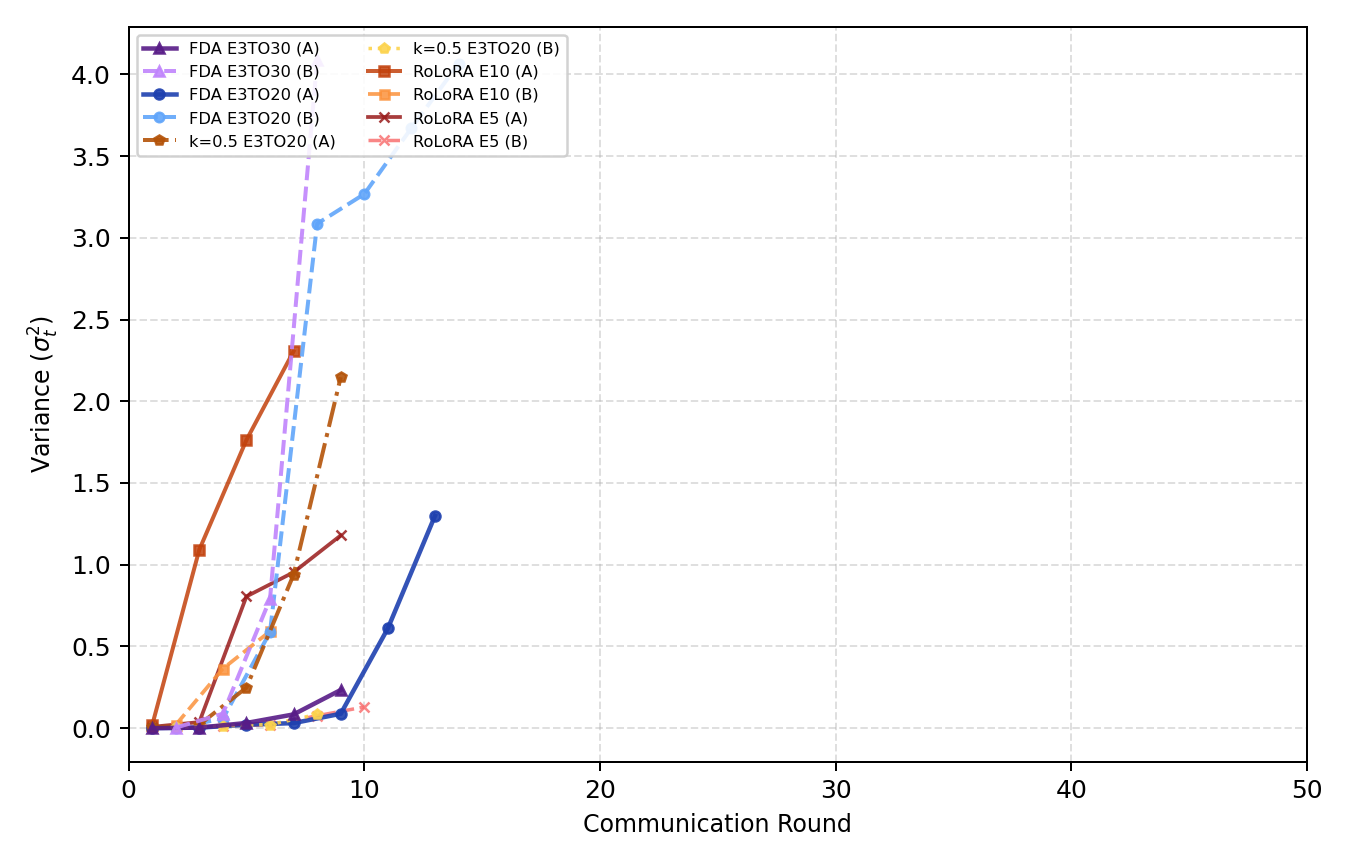
\includegraphics[width=\textwidth,height=4.9cm,keepaspectratio]{figures/telemetry/09_QQP_C20_R50_LR0.1_3_client_variance.png}
            \vspace{2pt}
            \par{\footnotesize \textbf{(e)} Subspace Coordinate Variance}
        \end{minipage}\hfill
        \begin{minipage}[b]{0.485\textwidth}
            \centering
            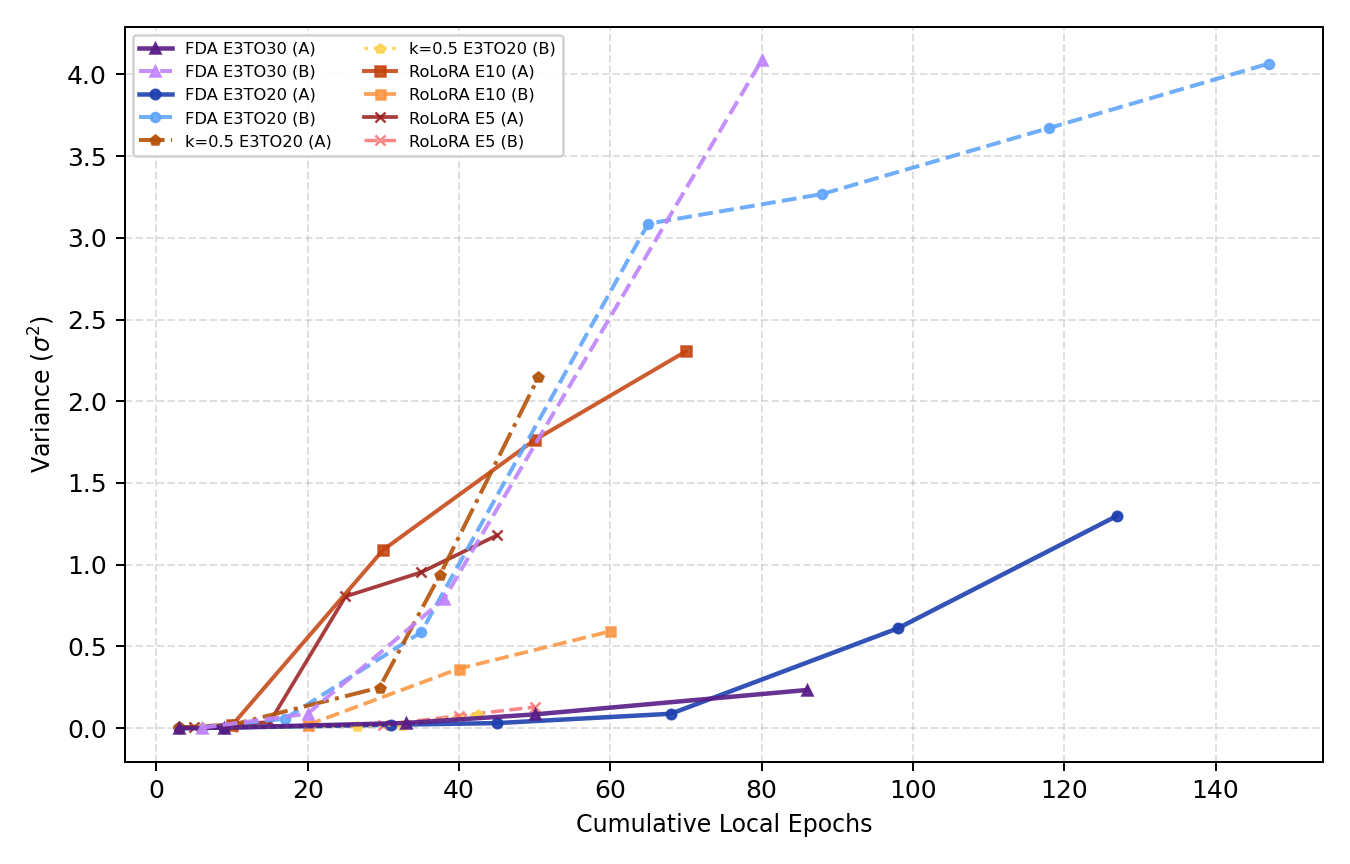
\includegraphics[width=\textwidth,height=4.9cm,keepaspectratio]{figures/telemetry/09_QQP_C20_R50_LR0.1_6_variance_vs_epoch.png}
            \vspace{2pt}
            \par{\footnotesize \textbf{(f)} Variance vs.\ Cumulative Local Epochs}
        \end{minipage}

        \vspace{0.6em}
        \caption{Multi-panel optimization telemetry on QQP ($C=20, R_{\max}=50, \eta_c=0.1, \alpha=1000.0$) comparing FDA-RoLoRA against static RoLoRA baselines under homogeneous consensus.}
        \label{fig:telemetry_qqp_c20_iid}
    \end{minipage}%
    }
\end{figure}

\begin{figure}[p]
    \centering
    \makebox[\textwidth][c]{%
    \begin{minipage}{1.06\textwidth}
        \begin{minipage}[b]{0.485\textwidth}
            \centering
            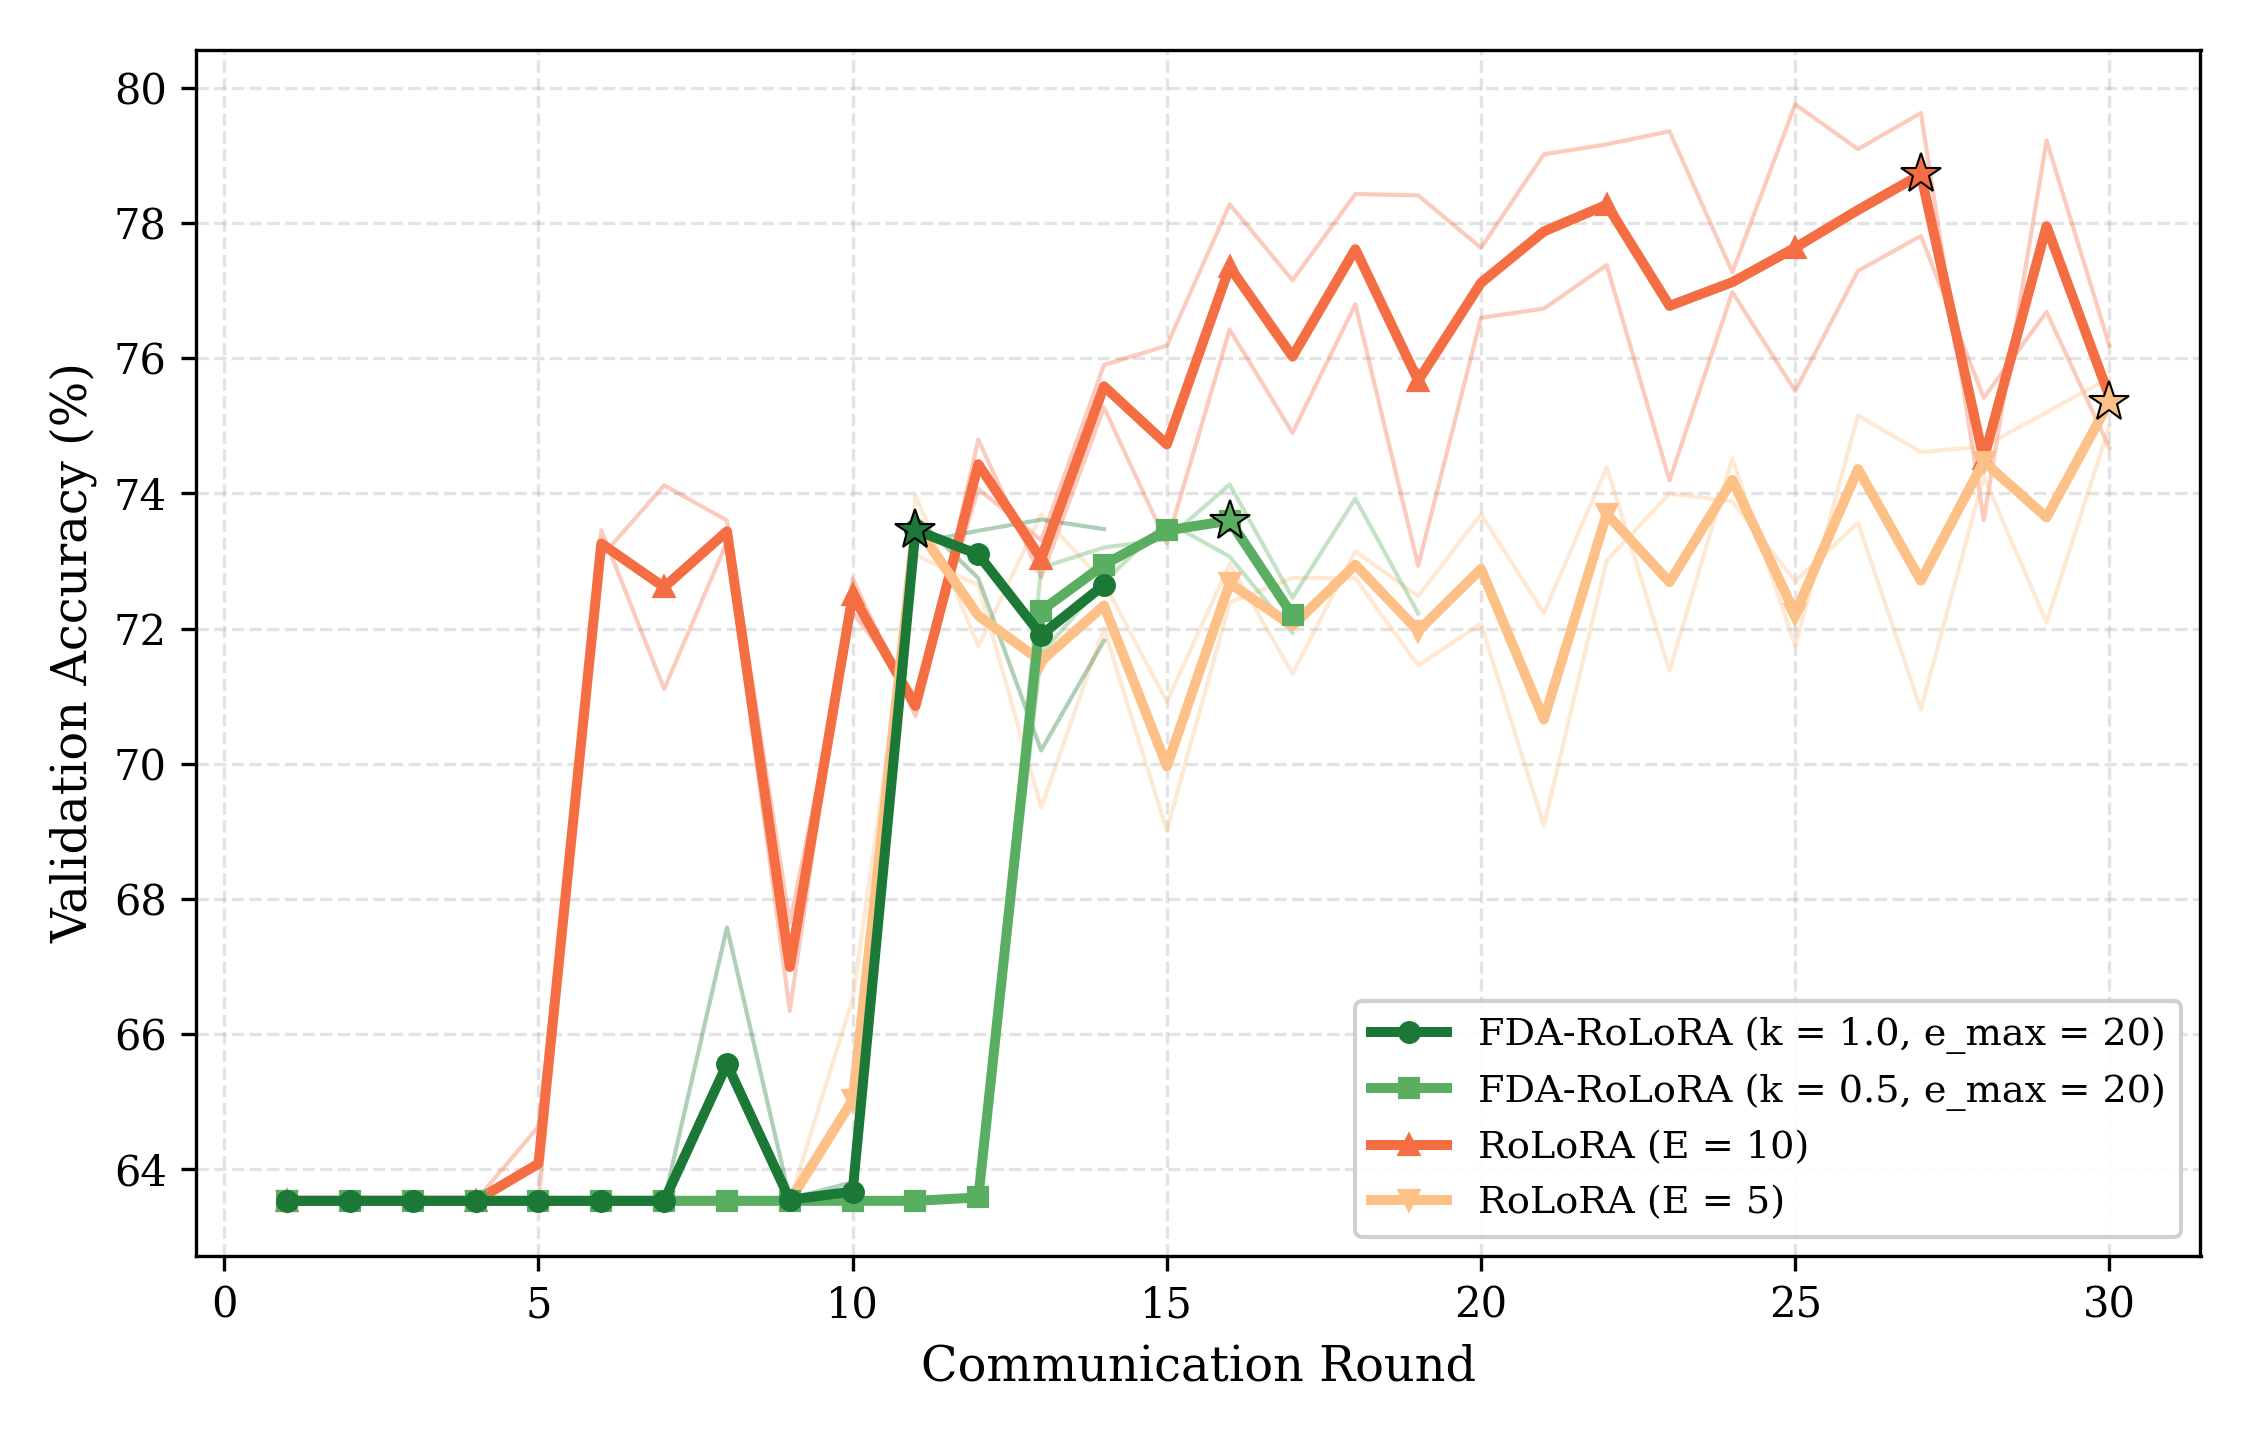
\includegraphics[width=\textwidth,height=4.9cm,keepaspectratio]{figures/telemetry/10_QQP_C50_R30_LR0.1_1_accuracy.png}
            \vspace{2pt}
            \par{\footnotesize \textbf{(a)} Validation Accuracy}
        \end{minipage}\hfill
        \begin{minipage}[b]{0.485\textwidth}
            \centering
            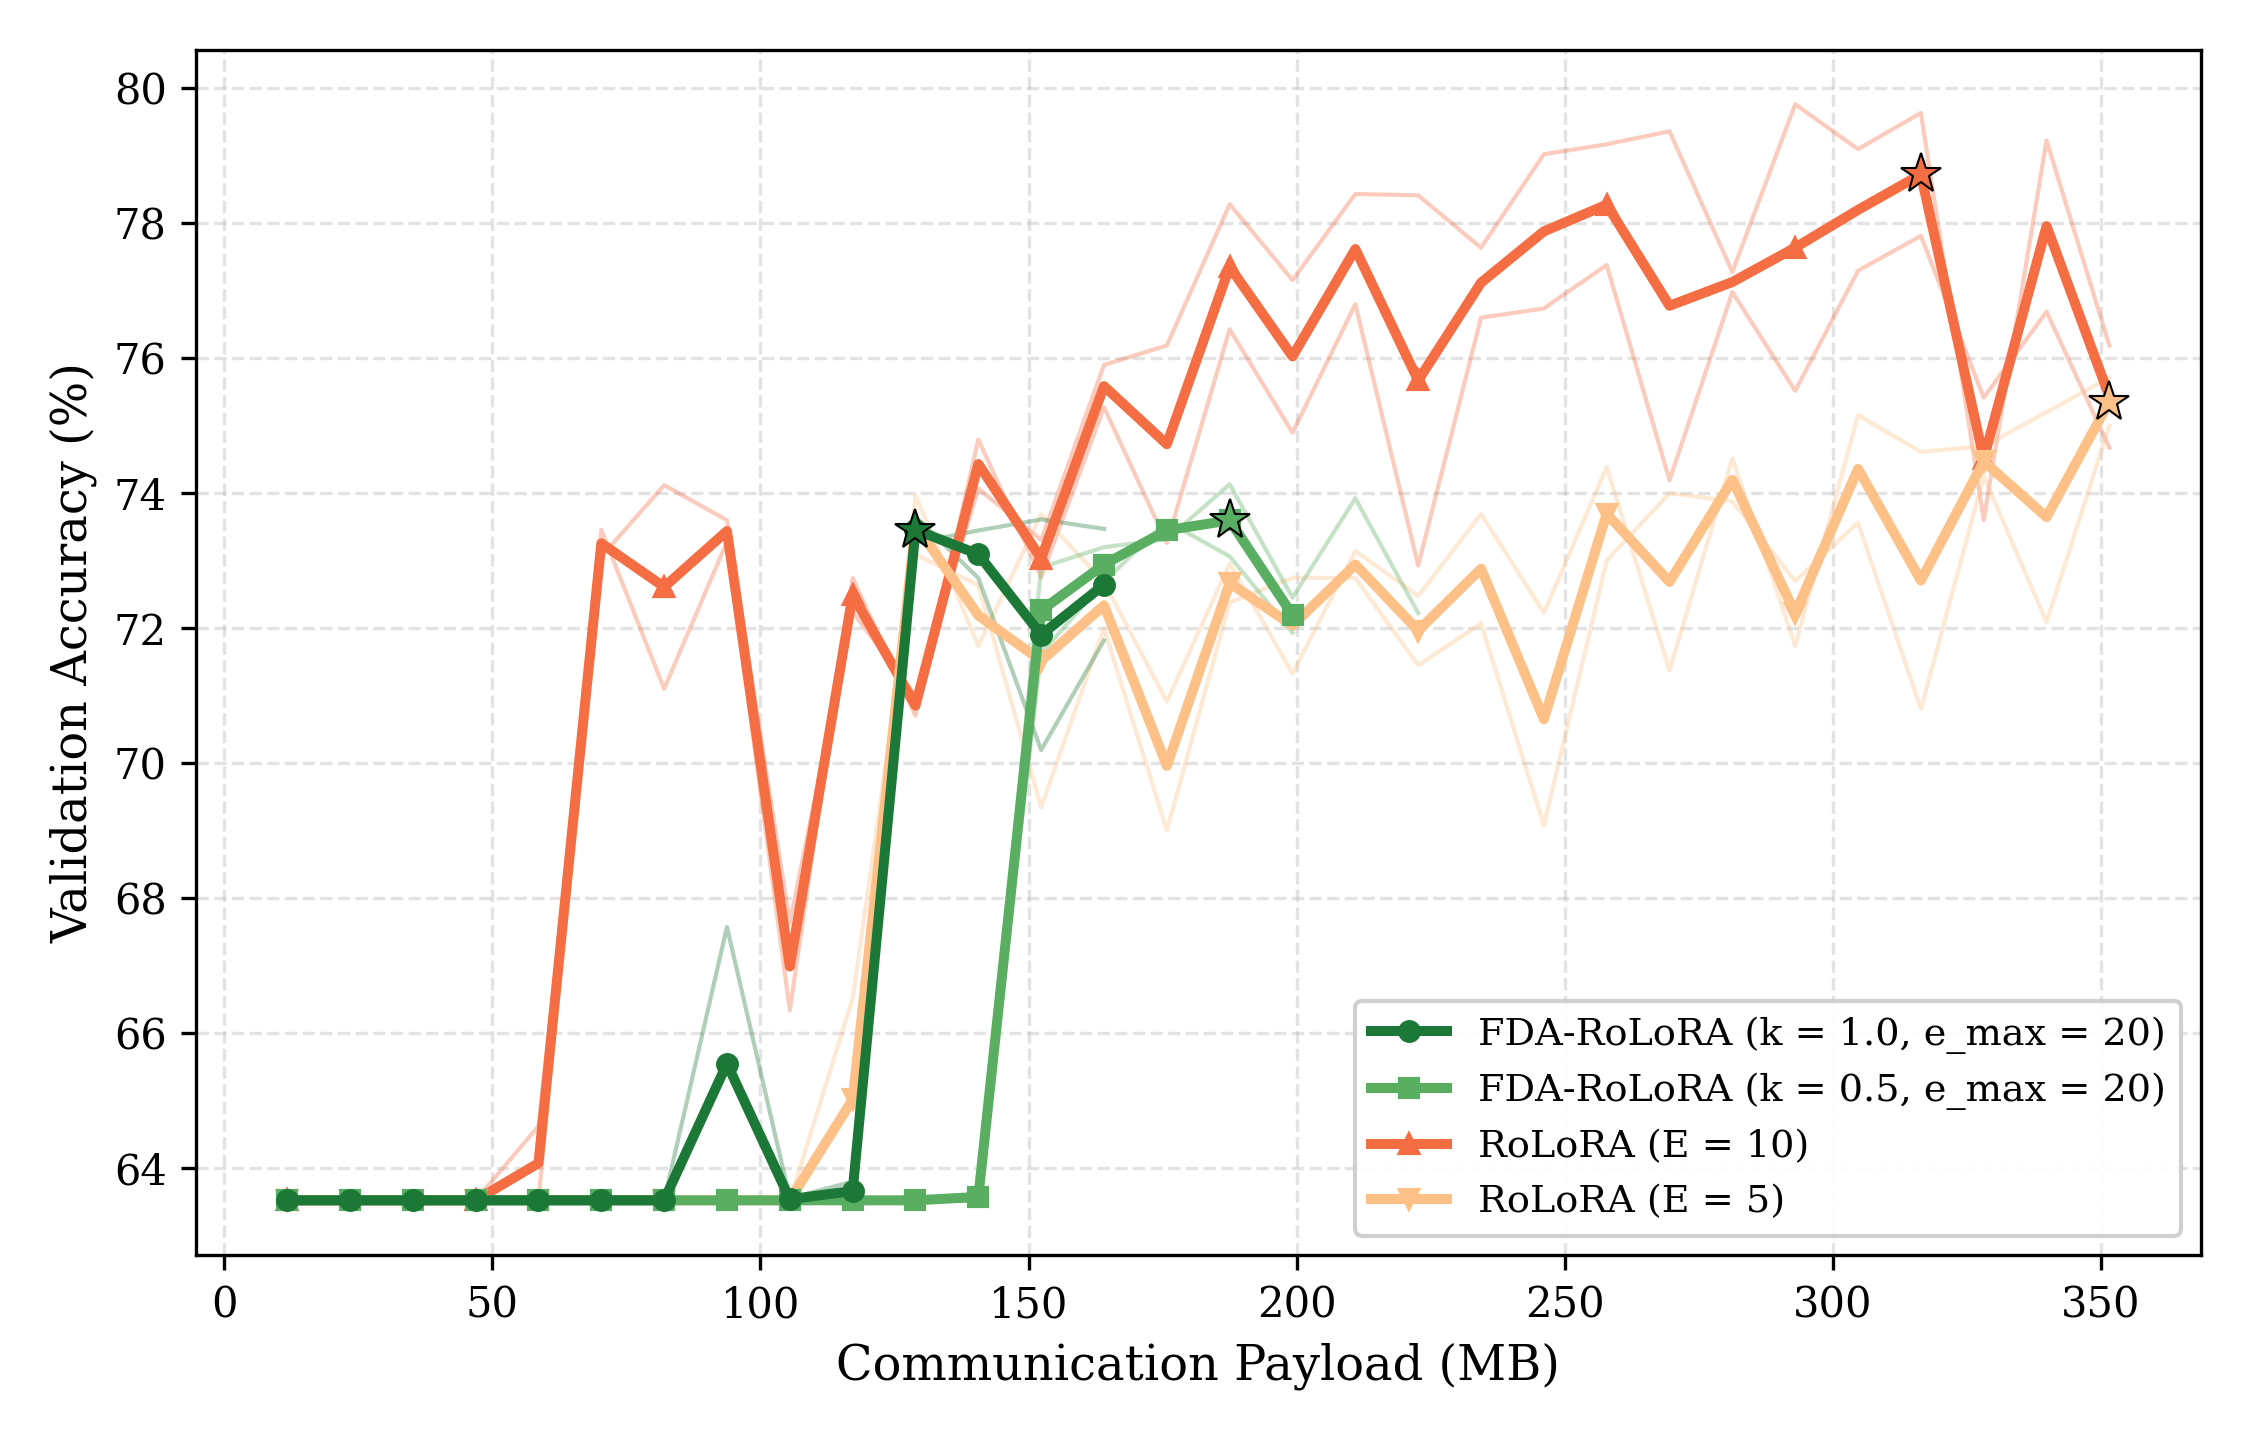
\includegraphics[width=\textwidth,height=4.9cm,keepaspectratio]{figures/telemetry/10_QQP_C50_R30_LR0.1_4_accuracy_vs_cost.png}
            \vspace{2pt}
            \par{\footnotesize \textbf{(b)} Accuracy vs. Communication (MB)}
        \end{minipage}

        \vspace{0.6em}
        \begin{minipage}[b]{0.485\textwidth}
            \centering
            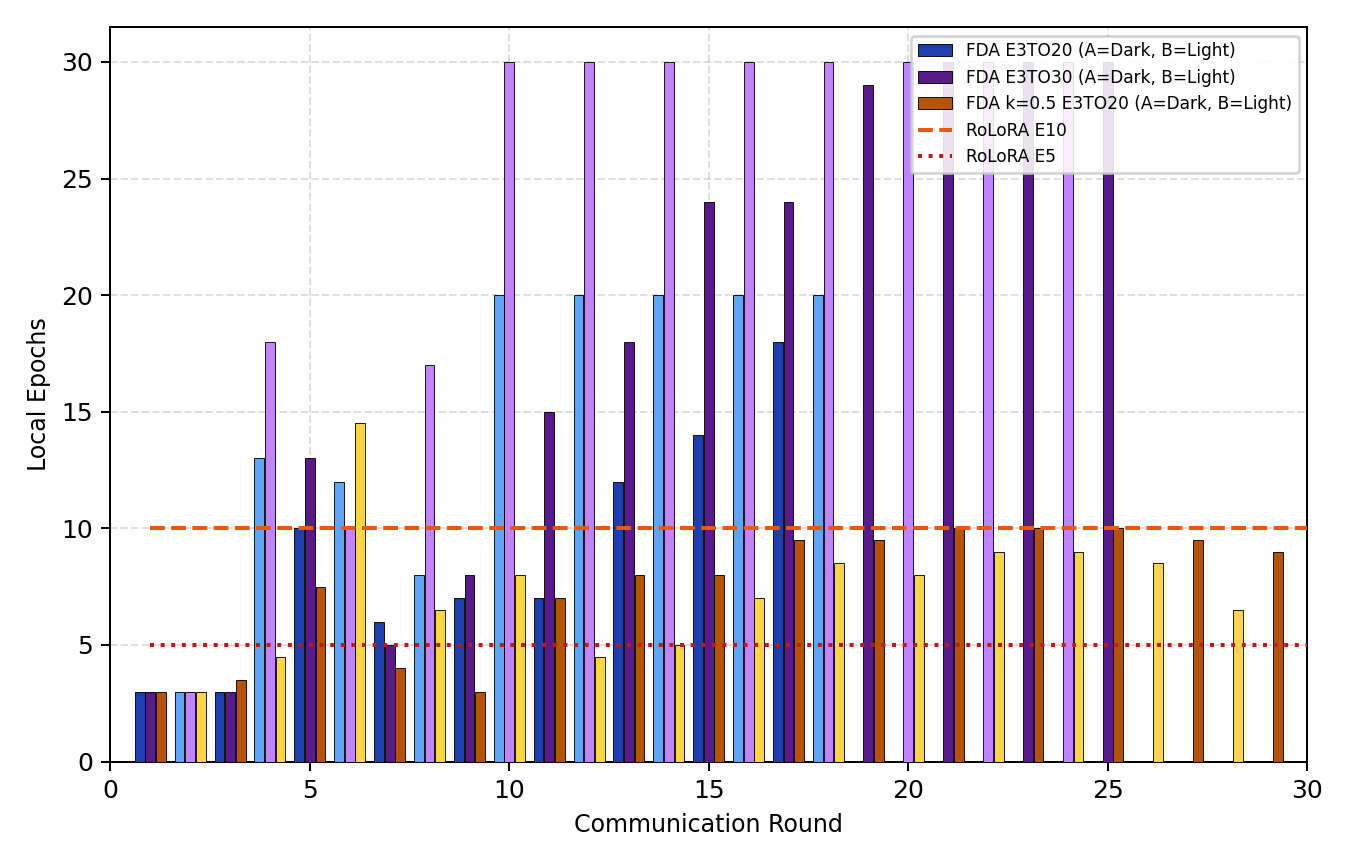
\includegraphics[width=\textwidth,height=4.9cm,keepaspectratio]{figures/telemetry/10_QQP_C50_R30_LR0.1_2_allocated_epochs.png}
            \vspace{2pt}
            \par{\footnotesize \textbf{(c)} Dynamic Local Epochs ($\bar{e}$)}
        \end{minipage}\hfill
        \begin{minipage}[b]{0.485\textwidth}
            \centering
            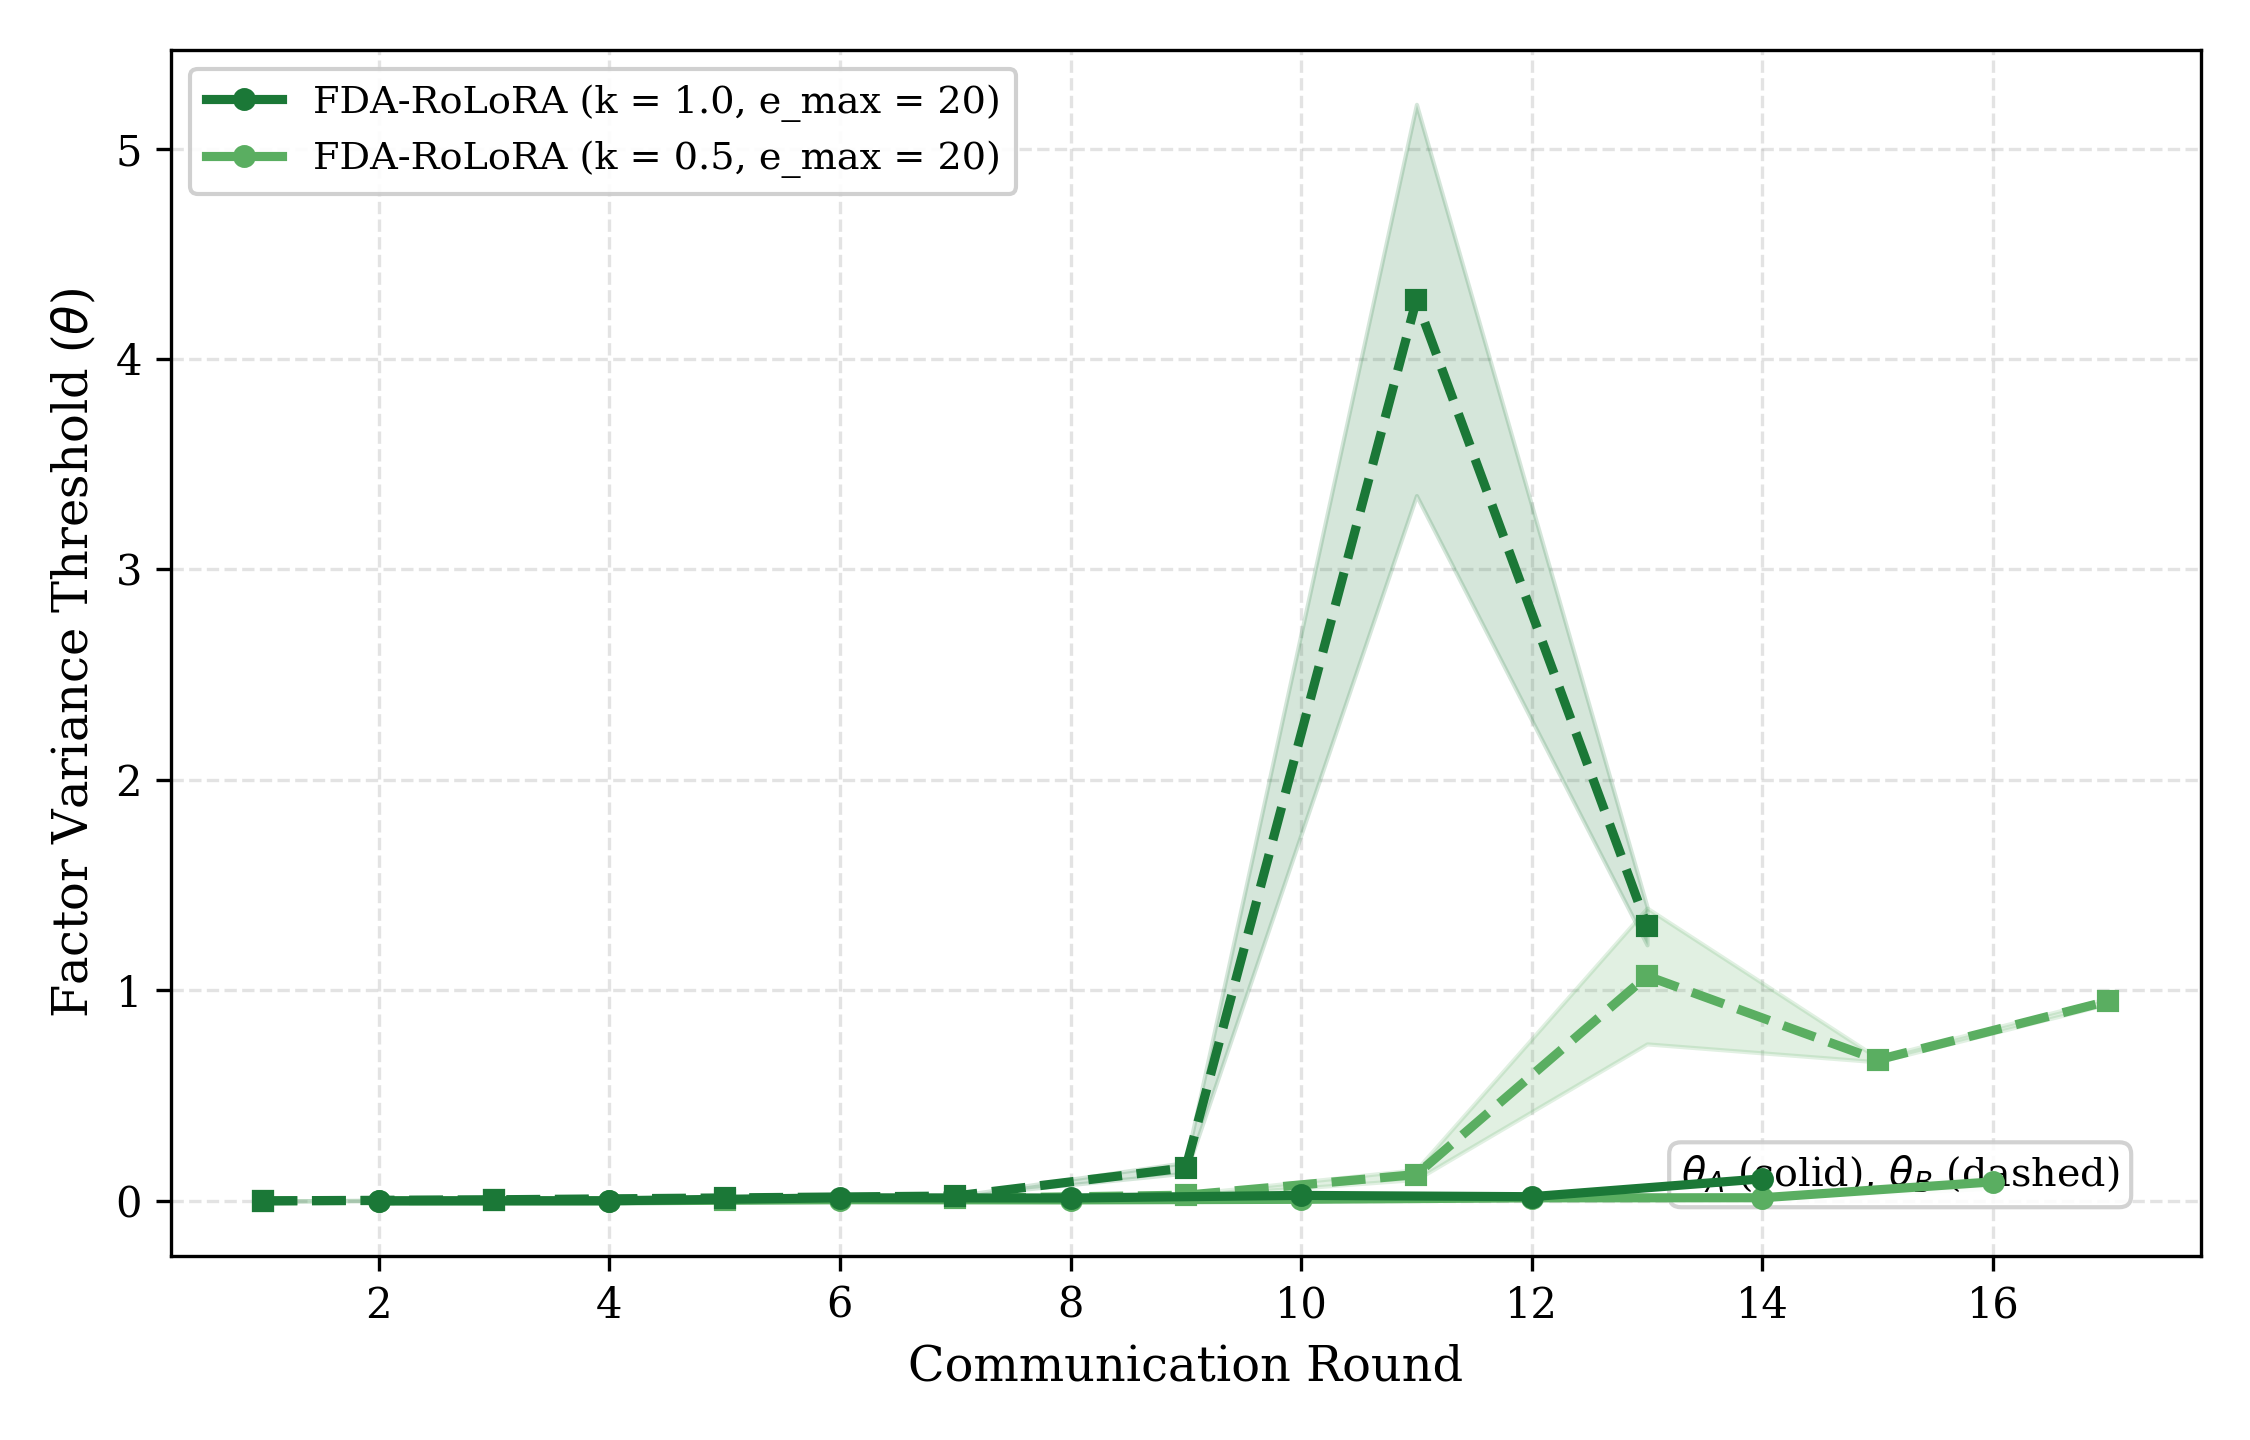
\includegraphics[width=\textwidth,height=4.9cm,keepaspectratio]{figures/telemetry/10_QQP_C50_R30_LR0.1_5_fda_threshold.png}
            \vspace{2pt}
            \par{\footnotesize \textbf{(d)} Factor Thresholds ($\theta_A, \theta_B$)}
        \end{minipage}

        \vspace{0.6em}
        \begin{minipage}[b]{0.485\textwidth}
            \centering
            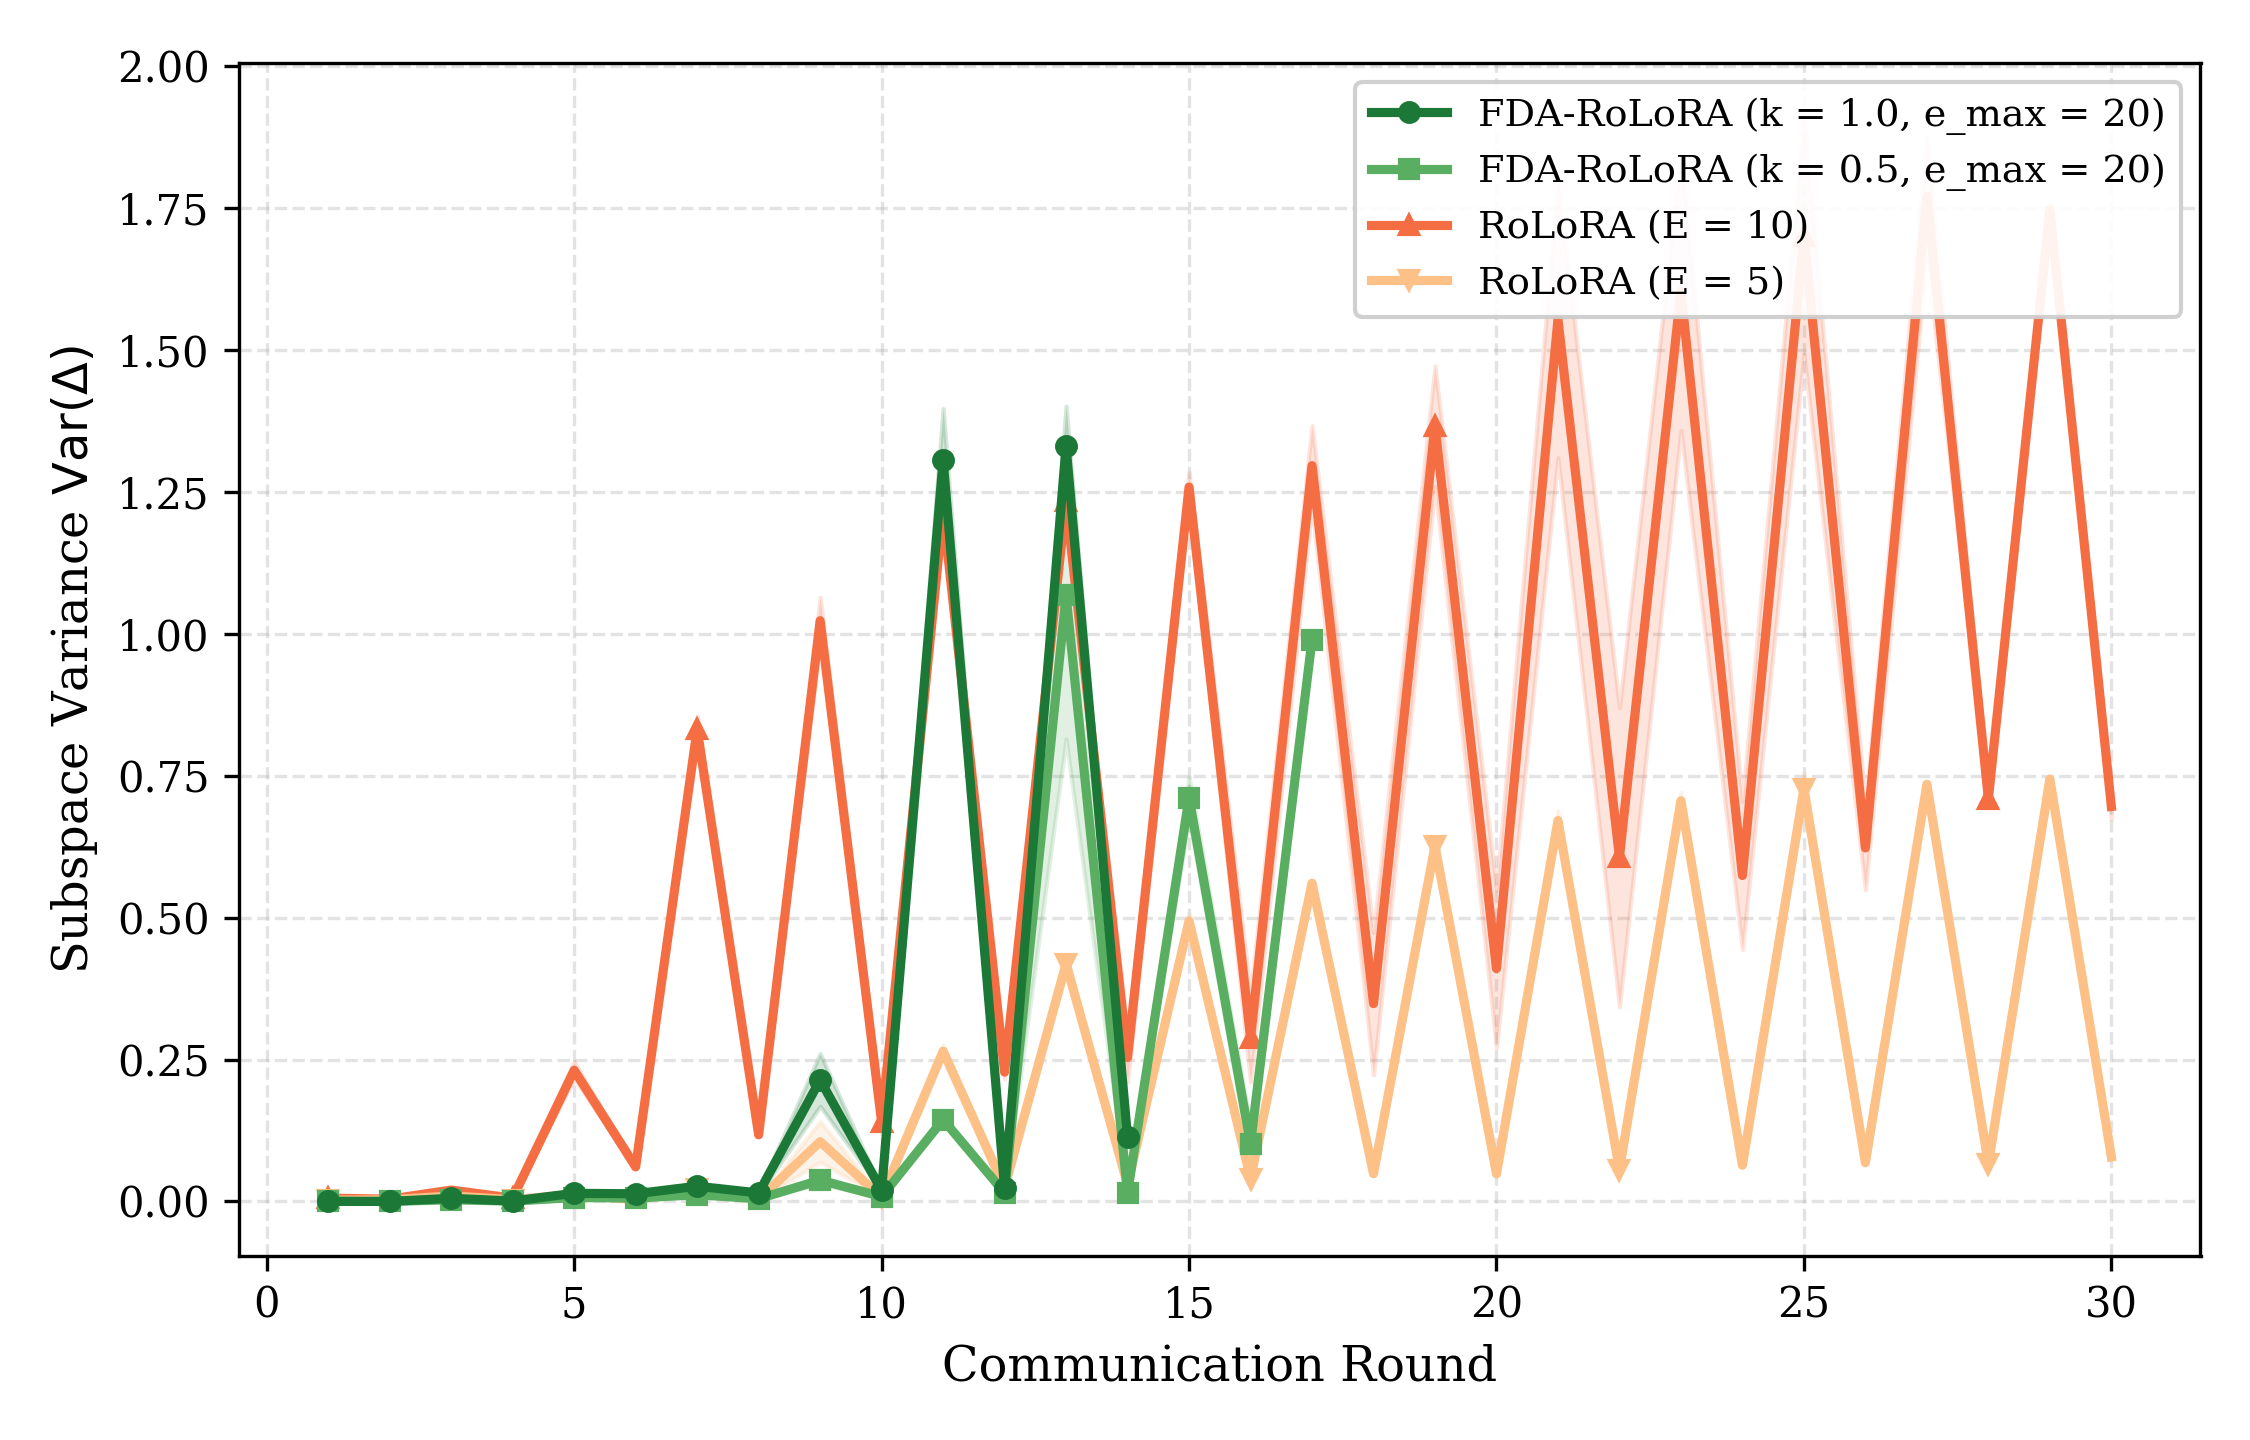
\includegraphics[width=\textwidth,height=4.9cm,keepaspectratio]{figures/telemetry/10_QQP_C50_R30_LR0.1_3_client_variance.png}
            \vspace{2pt}
            \par{\footnotesize \textbf{(e)} Subspace Coordinate Variance}
        \end{minipage}\hfill
        \begin{minipage}[b]{0.485\textwidth}
            \centering
            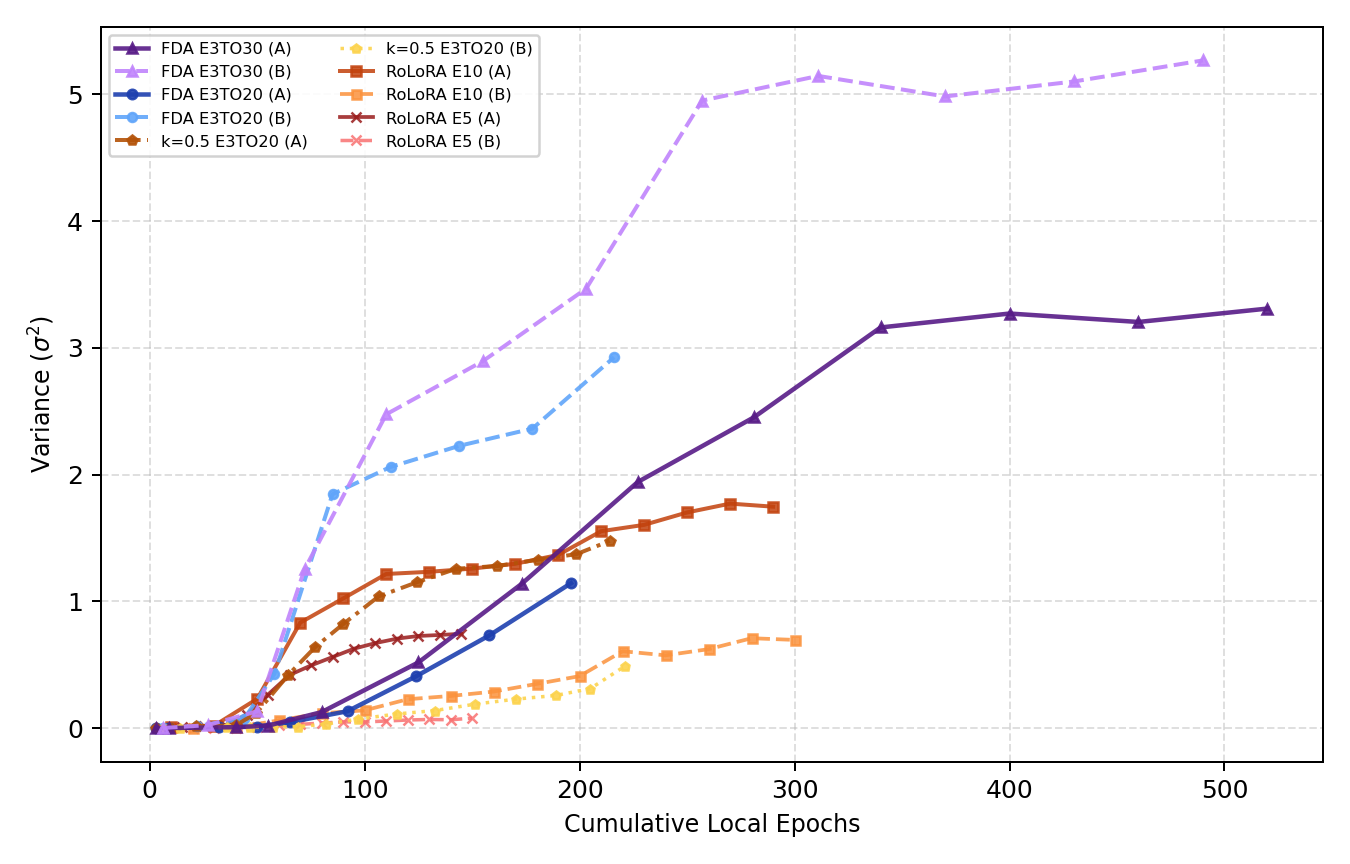
\includegraphics[width=\textwidth,height=4.9cm,keepaspectratio]{figures/telemetry/10_QQP_C50_R30_LR0.1_6_variance_vs_epoch.png}
            \vspace{2pt}
            \par{\footnotesize \textbf{(f)} Variance vs.\ Cumulative Local Epochs}
        \end{minipage}

        \vspace{0.6em}
        \caption{Multi-panel optimization telemetry on QQP ($C=50, R_{\max}=30, \eta_c=0.1, \alpha=1000.0$) under expanded cohort scale $C=50$.}
        \label{fig:telemetry_qqp_c50_iid}
    \end{minipage}%
    }
\end{figure}

\paragraph{SST-2:}
Figures~\ref{fig:telemetry_sst2_c20_iid} and \ref{fig:telemetry_sst2_c50_iid} report telemetry on single-sentence sentiment classification under homogeneous consensus. On $C=20$ (Figure~\ref{fig:telemetry_sst2_c20_iid}), both FDA-RoLoRA and fixed RoLoRA rapidly cross $92\%$ validation accuracy (Panel a). FDA-RoLoRA ($k=1.0$) reaches a peak of $92.14\%$, close to RoLoRA $E=20$ ($92.55\%$), but uses more communication ($57.7\,\text{MB}$ vs.\ $30.0\,\text{MB}$). Realized local epochs (Panel c) settle at $\bar{e} = 11.11$ per round, while dual thresholds (Panel d) stabilize at tight equilibria. Round-level drift variance (Panel e) is bounded at $\bar{\nu} = 0.654$.

On $C=50$ (Figure~\ref{fig:telemetry_sst2_c50_iid}), FDA-RoLoRA ($k=1.0$) achieves $89.68\%$ validation accuracy in $20.0$ rounds ($140.6\,\text{MB}$) versus $22.0$ rounds ($154.7\,\text{MB}$) for static RoLoRA $E=10$ (Panels a \& b), at lower accuracy than RoLoRA $E=10$ ($90.54\%$ peak) and $E=20$ ($92.01\%$ peak). Cohort aggregation suppresses coordinate drift variance to a low $\bar{\nu} = 0.063$ (Panel e).
\begin{figure}[p]
    \centering
    \makebox[\textwidth][c]{%
    \begin{minipage}{1.06\textwidth}
        \begin{minipage}[b]{0.485\textwidth}
            \centering
            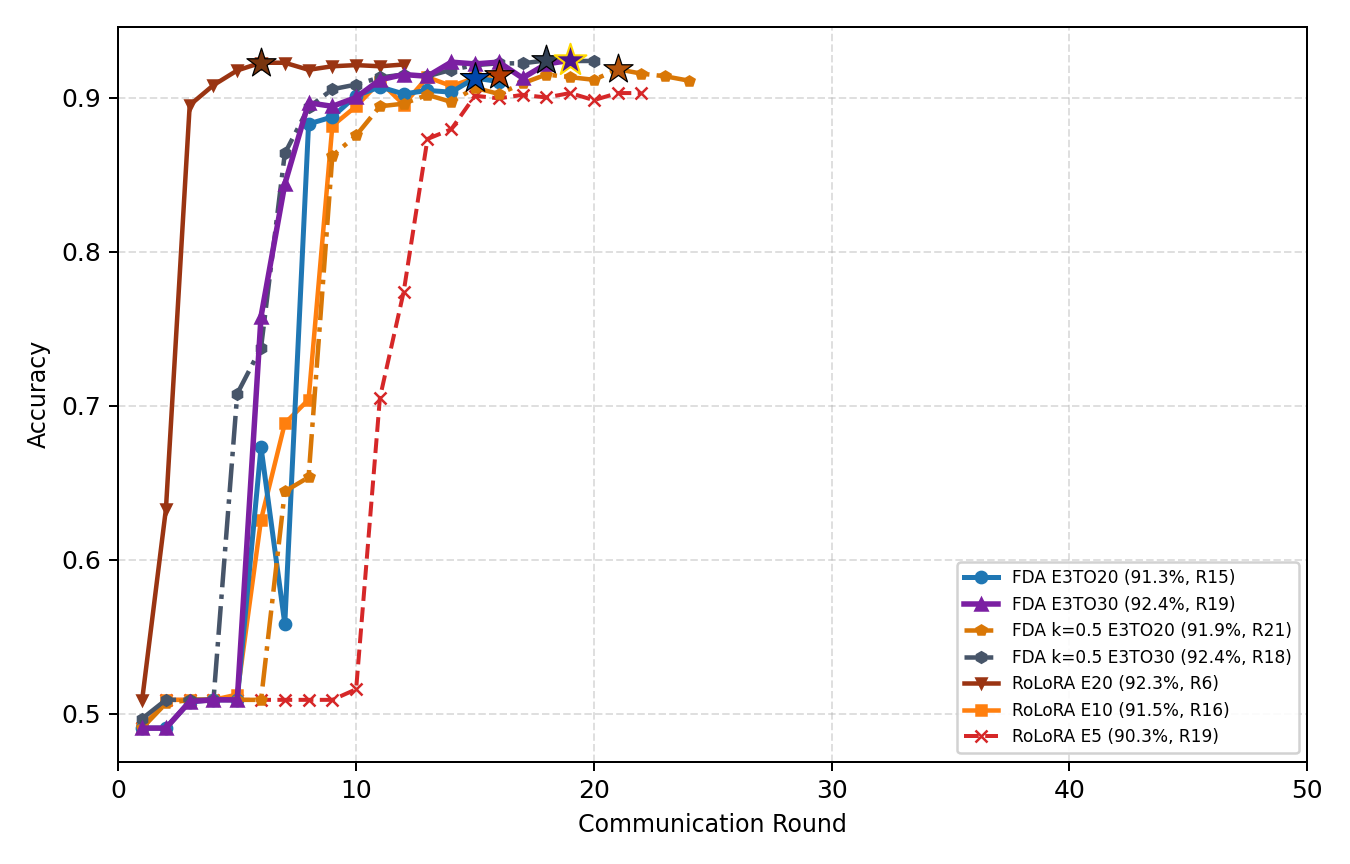
\includegraphics[width=\textwidth,height=4.9cm,keepaspectratio]{figures/telemetry/11_SST2_C20_R50_LR0.1_1_accuracy.png}
            \vspace{2pt}
            \par{\footnotesize \textbf{(a)} Validation Accuracy}
        \end{minipage}\hfill
        \begin{minipage}[b]{0.485\textwidth}
            \centering
            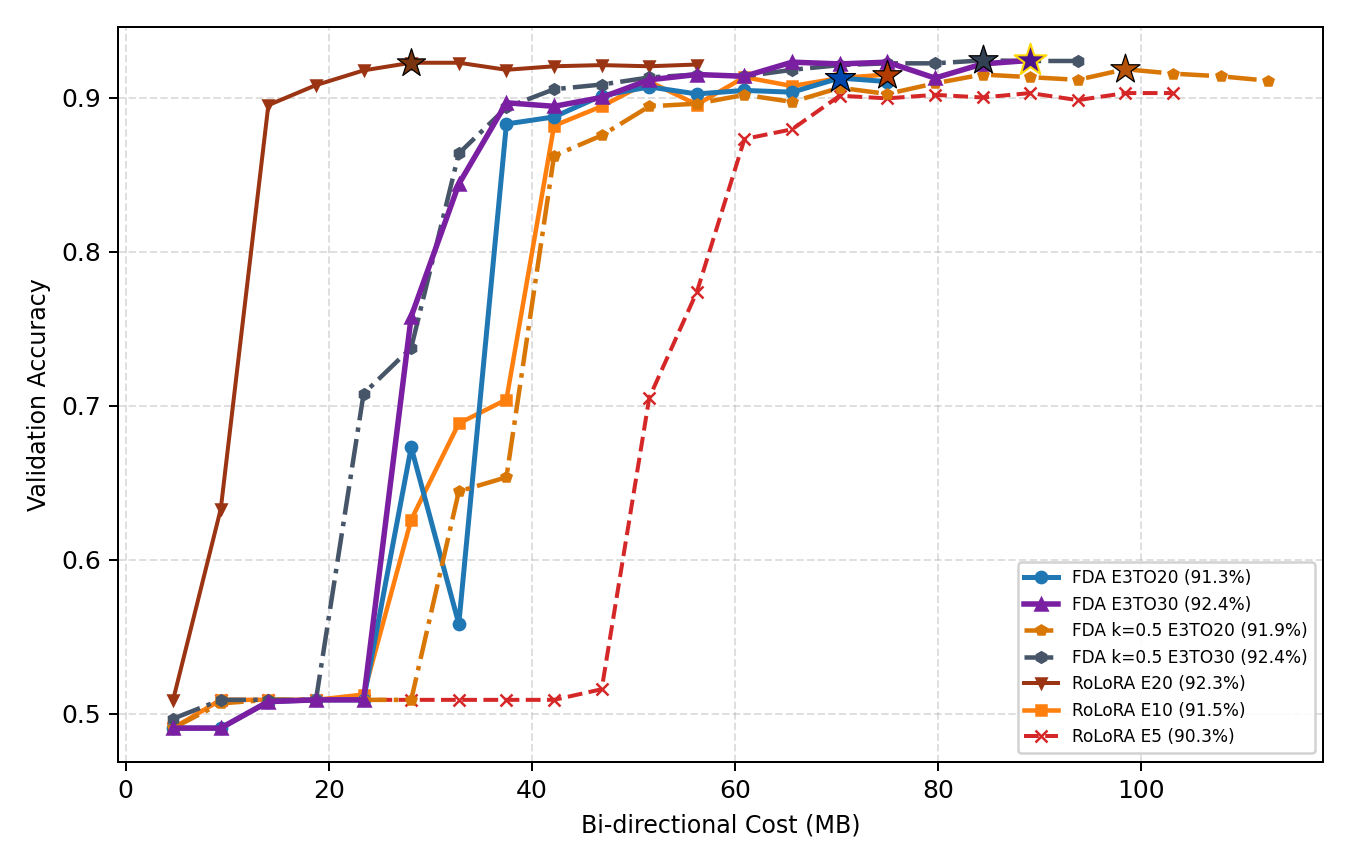
\includegraphics[width=\textwidth,height=4.9cm,keepaspectratio]{figures/telemetry/11_SST2_C20_R50_LR0.1_4_accuracy_vs_cost.png}
            \vspace{2pt}
            \par{\footnotesize \textbf{(b)} Accuracy vs. Communication (MB)}
        \end{minipage}

        \vspace{0.6em}
        \begin{minipage}[b]{0.485\textwidth}
            \centering
            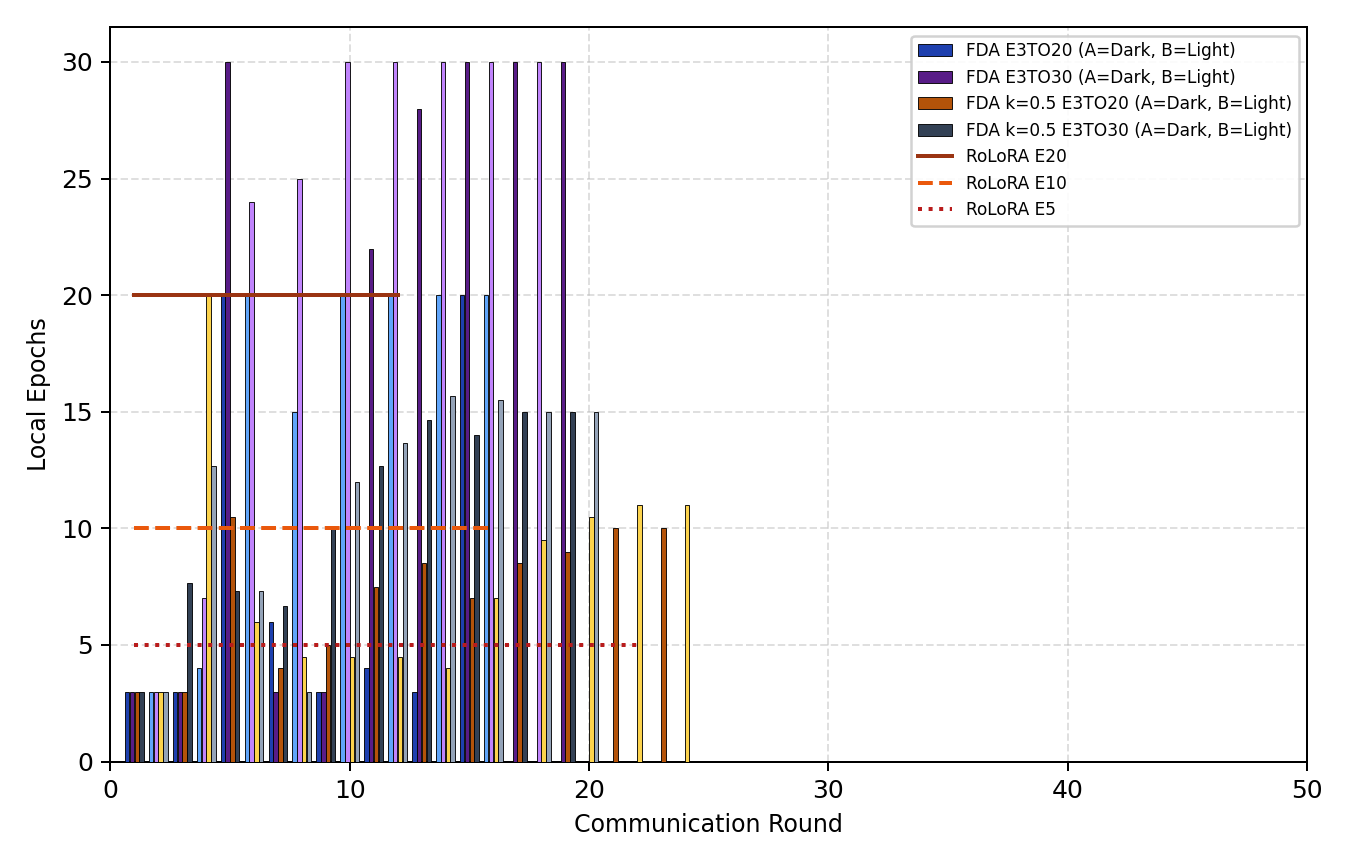
\includegraphics[width=\textwidth,height=4.9cm,keepaspectratio]{figures/telemetry/11_SST2_C20_R50_LR0.1_2_allocated_epochs.png}
            \vspace{2pt}
            \par{\footnotesize \textbf{(c)} Dynamic Local Epochs ($\bar{e}$)}
        \end{minipage}\hfill
        \begin{minipage}[b]{0.485\textwidth}
            \centering
            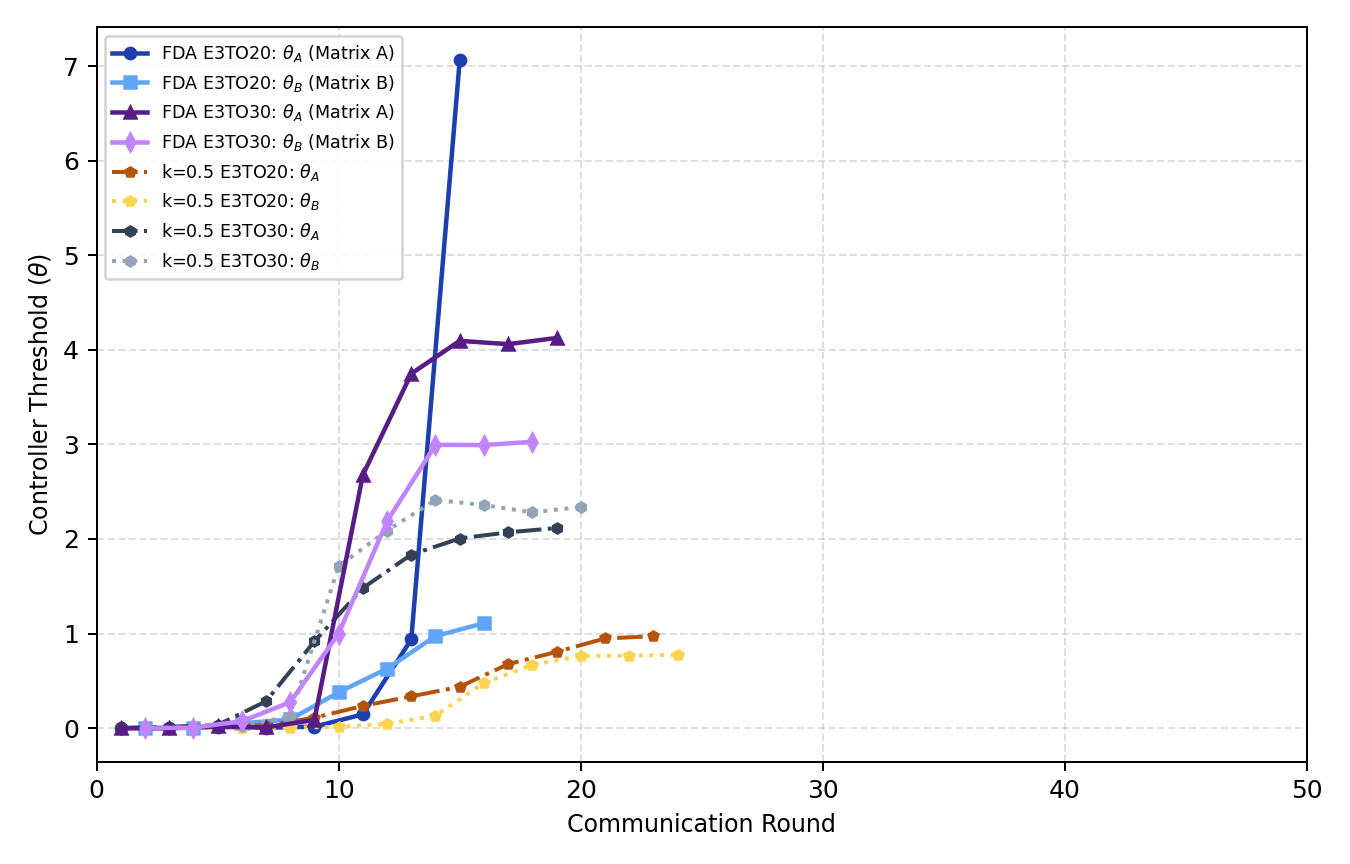
\includegraphics[width=\textwidth,height=4.9cm,keepaspectratio]{figures/telemetry/11_SST2_C20_R50_LR0.1_5_fda_threshold.png}
            \vspace{2pt}
            \par{\footnotesize \textbf{(d)} Factor Thresholds ($\theta_A, \theta_B$)}
        \end{minipage}

        \vspace{0.6em}
        \begin{minipage}[b]{0.485\textwidth}
            \centering
            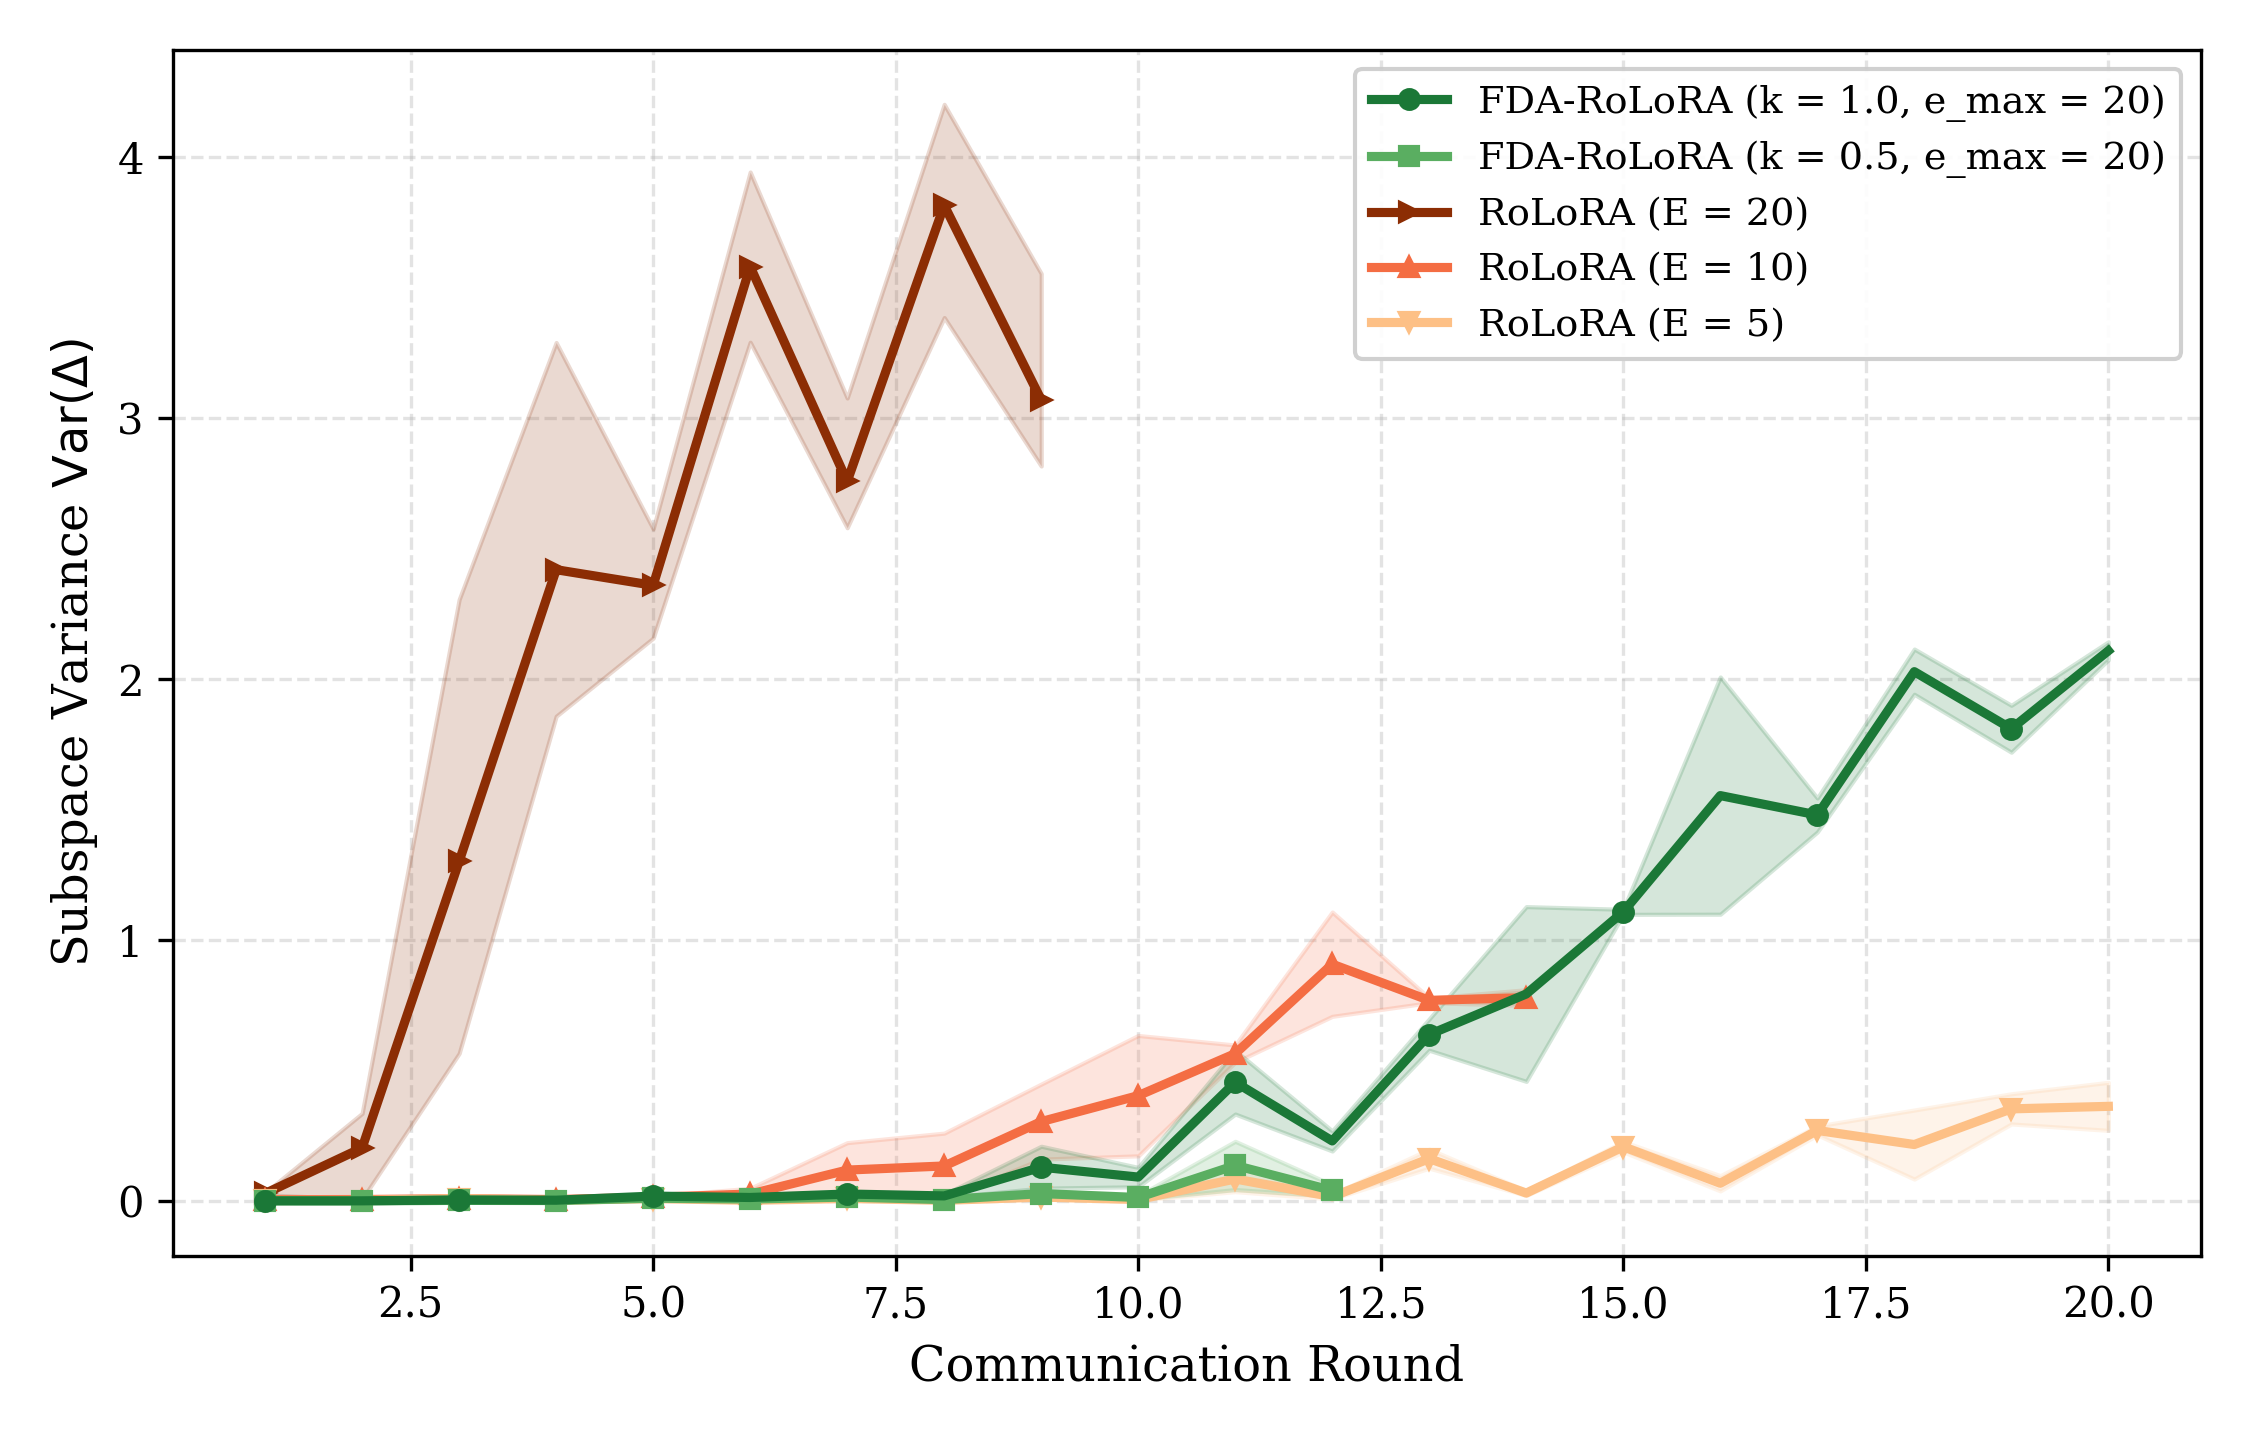
\includegraphics[width=\textwidth,height=4.9cm,keepaspectratio]{figures/telemetry/11_SST2_C20_R50_LR0.1_3_client_variance.png}
            \vspace{2pt}
            \par{\footnotesize \textbf{(e)} Subspace Coordinate Variance}
        \end{minipage}\hfill
        \begin{minipage}[b]{0.485\textwidth}
            \centering
            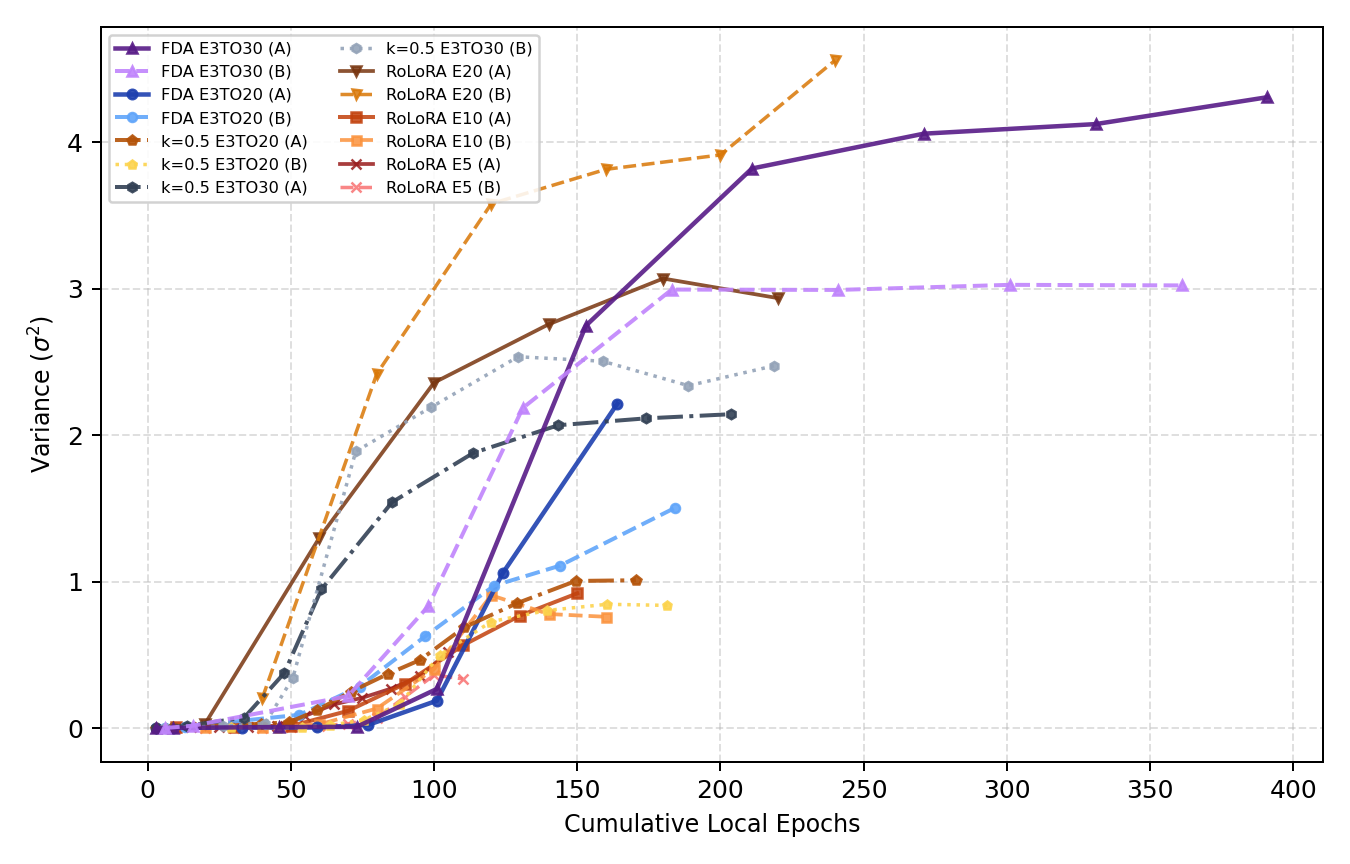
\includegraphics[width=\textwidth,height=4.9cm,keepaspectratio]{figures/telemetry/11_SST2_C20_R50_LR0.1_6_variance_vs_epoch.png}
            \vspace{2pt}
            \par{\footnotesize \textbf{(f)} Variance vs.\ Cumulative Local Epochs}
        \end{minipage}

        \vspace{0.6em}
        \caption{Multi-panel optimization telemetry on SST-2 ($C=20, R_{\max}=50, \eta_c=0.1, \alpha=1000.0$) comparing FDA-RoLoRA against static RoLoRA baselines under homogeneous consensus.}
        \label{fig:telemetry_sst2_c20_iid}
    \end{minipage}%
    }
\end{figure}

\begin{figure}[p]
    \centering
    \makebox[\textwidth][c]{%
    \begin{minipage}{1.06\textwidth}
        \begin{minipage}[b]{0.485\textwidth}
            \centering
            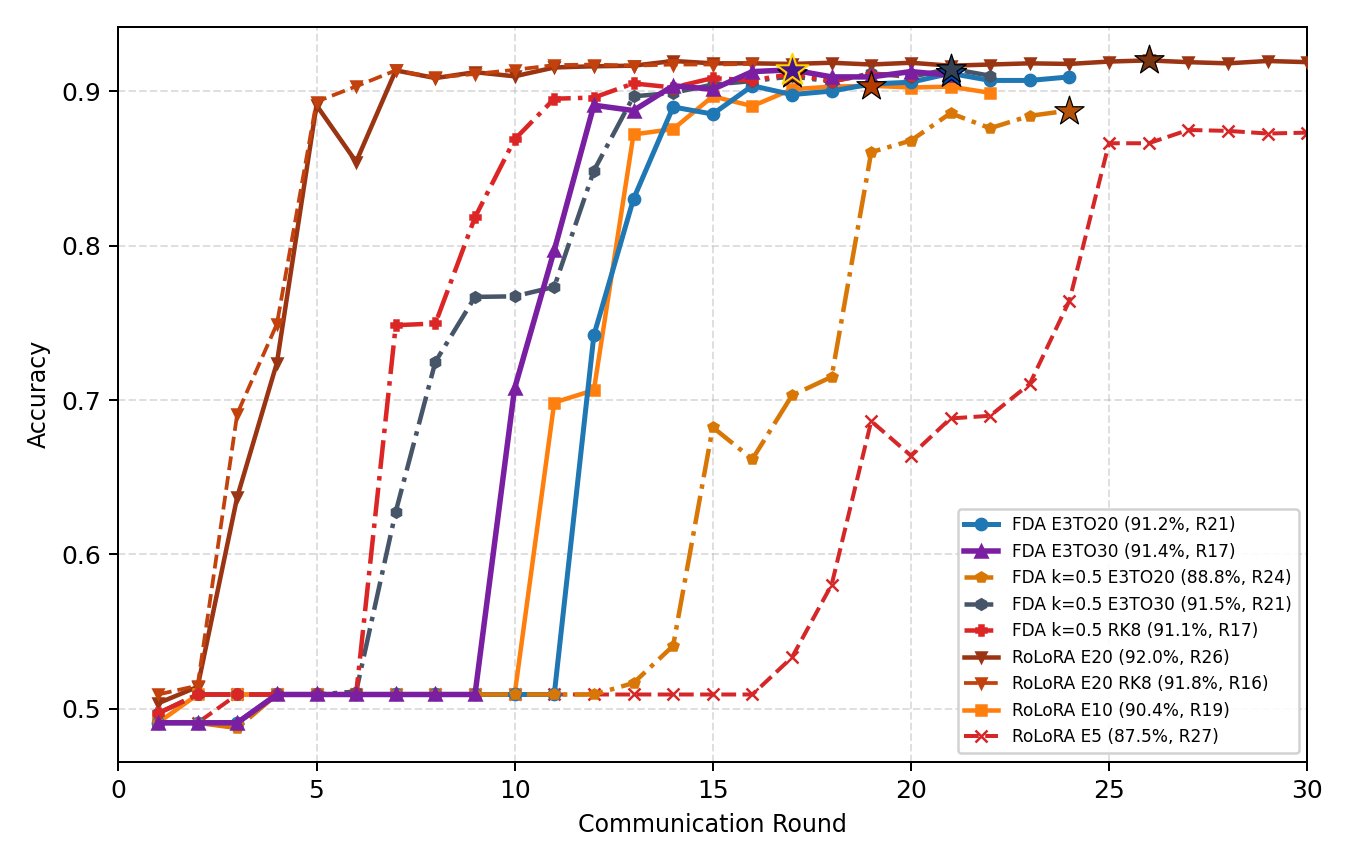
\includegraphics[width=\textwidth,height=4.9cm,keepaspectratio]{figures/telemetry/12_SST2_C50_R30_LR0.1_1_accuracy.png}
            \vspace{2pt}
            \par{\footnotesize \textbf{(a)} Validation Accuracy}
        \end{minipage}\hfill
        \begin{minipage}[b]{0.485\textwidth}
            \centering
            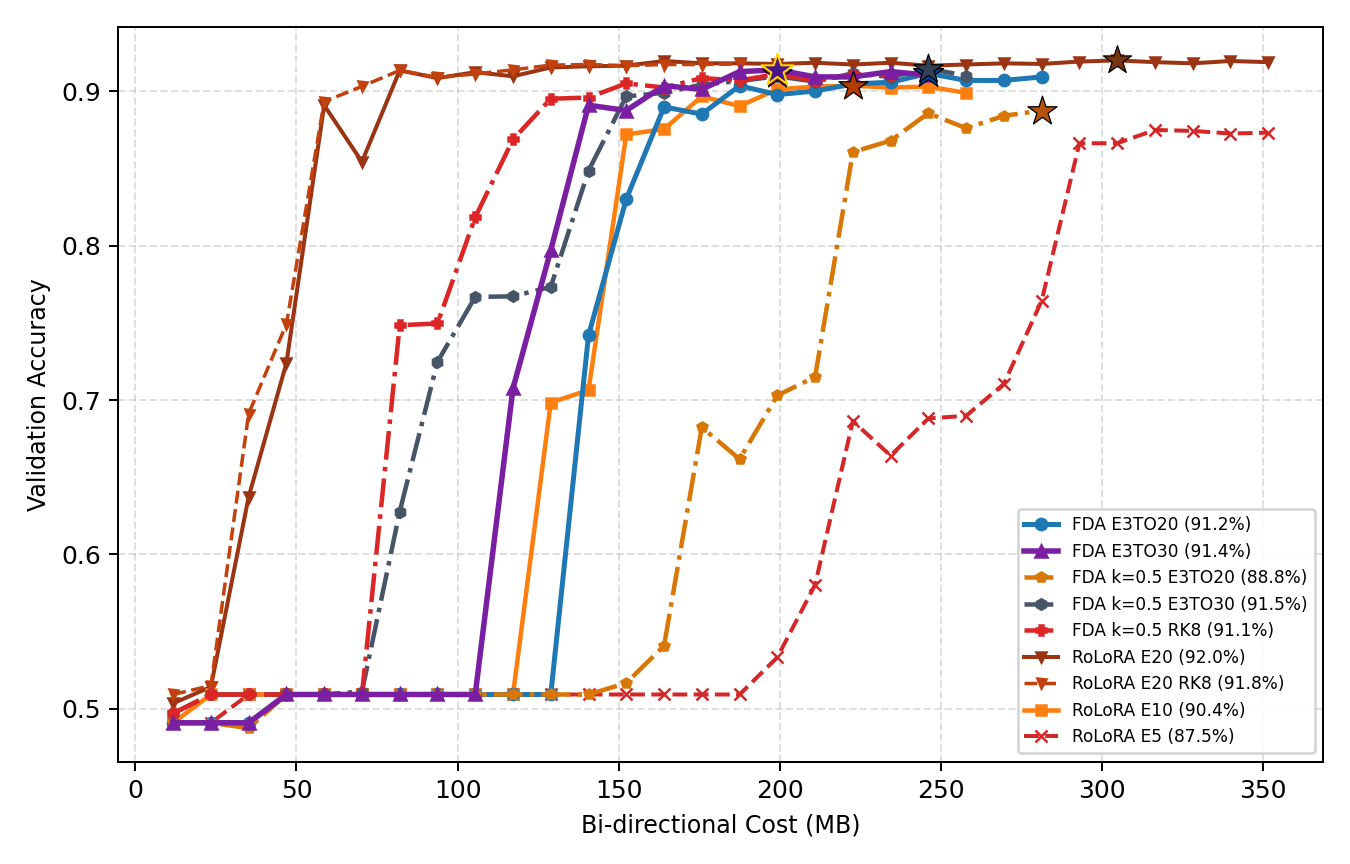
\includegraphics[width=\textwidth,height=4.9cm,keepaspectratio]{figures/telemetry/12_SST2_C50_R30_LR0.1_4_accuracy_vs_cost.png}
            \vspace{2pt}
            \par{\footnotesize \textbf{(b)} Accuracy vs. Communication (MB)}
        \end{minipage}

        \vspace{0.6em}
        \begin{minipage}[b]{0.485\textwidth}
            \centering
            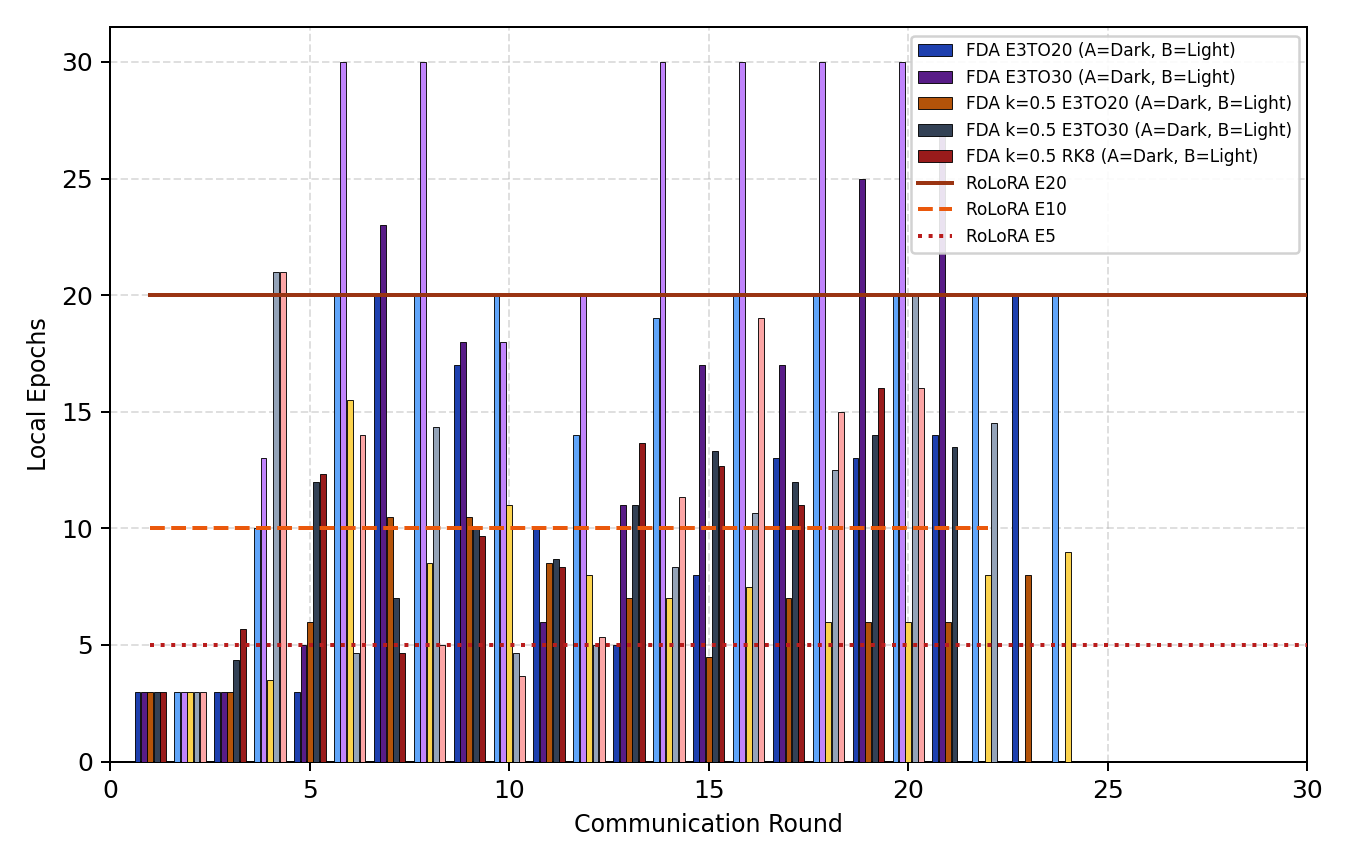
\includegraphics[width=\textwidth,height=4.9cm,keepaspectratio]{figures/telemetry/12_SST2_C50_R30_LR0.1_2_allocated_epochs.png}
            \vspace{2pt}
            \par{\footnotesize \textbf{(c)} Dynamic Local Epochs ($\bar{e}$)}
        \end{minipage}\hfill
        \begin{minipage}[b]{0.485\textwidth}
            \centering
            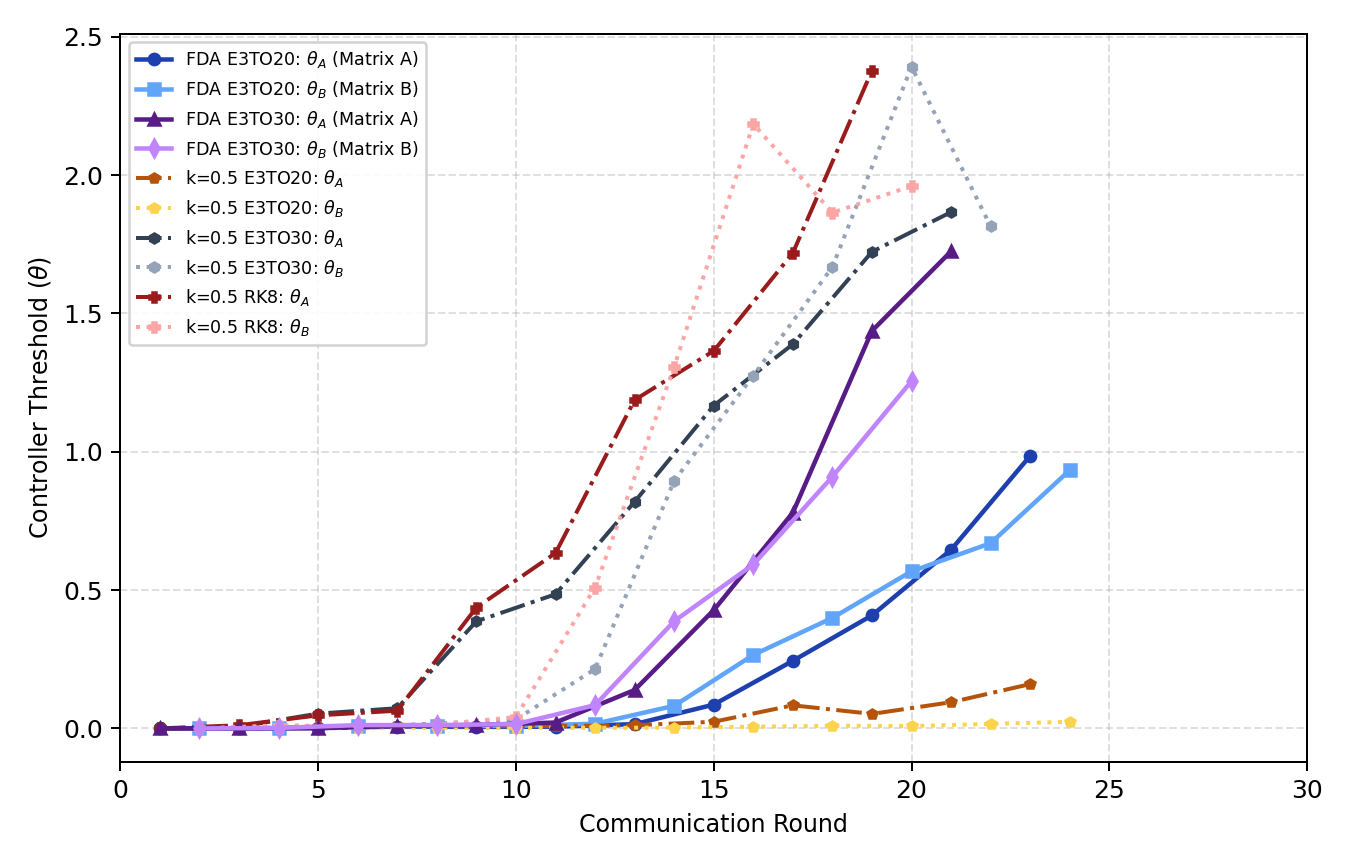
\includegraphics[width=\textwidth,height=4.9cm,keepaspectratio]{figures/telemetry/12_SST2_C50_R30_LR0.1_5_fda_threshold.png}
            \vspace{2pt}
            \par{\footnotesize \textbf{(d)} Factor Thresholds ($\theta_A, \theta_B$)}
        \end{minipage}

        \vspace{0.6em}
        \begin{minipage}[b]{0.485\textwidth}
            \centering
            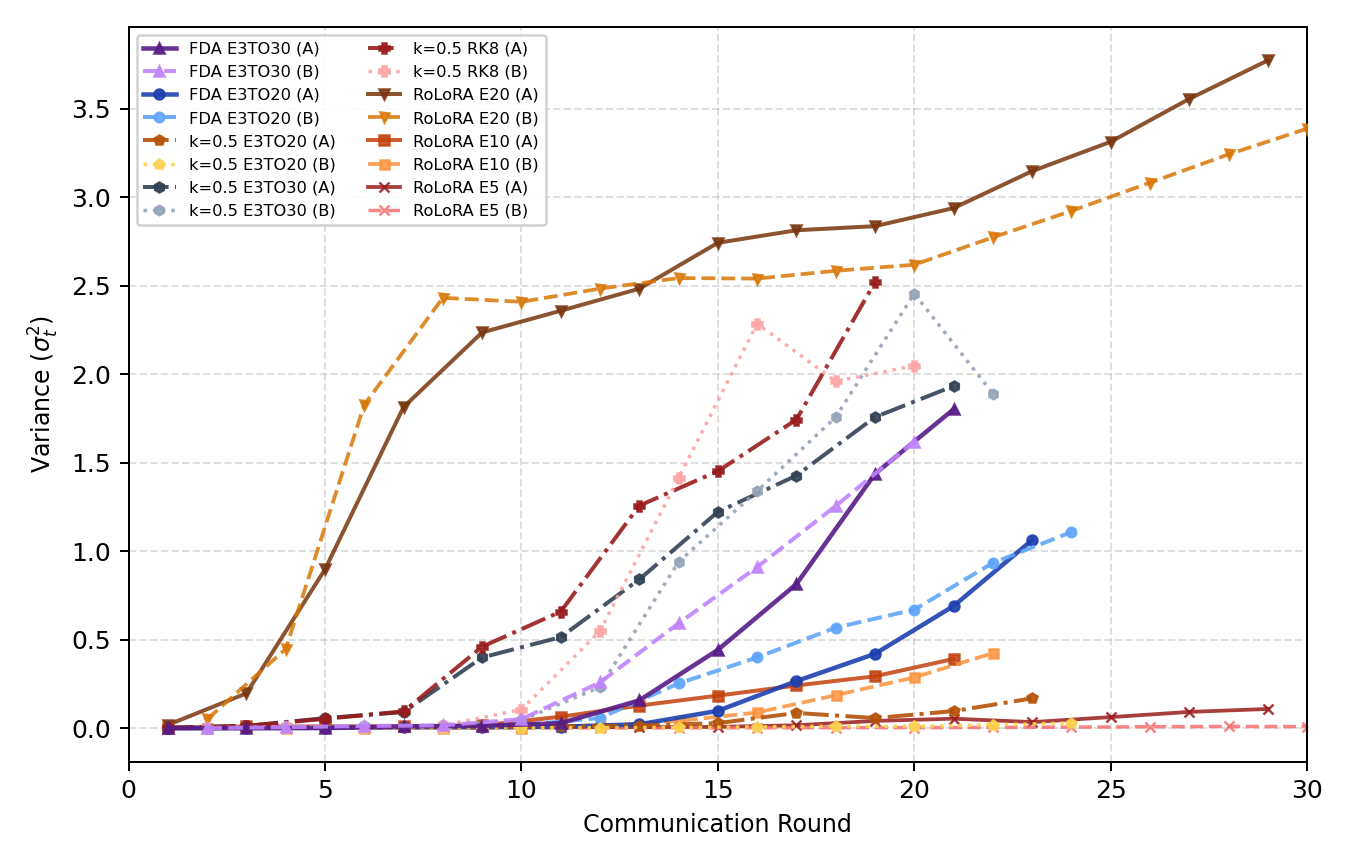
\includegraphics[width=\textwidth,height=4.9cm,keepaspectratio]{figures/telemetry/12_SST2_C50_R30_LR0.1_3_client_variance.png}
            \vspace{2pt}
            \par{\footnotesize \textbf{(e)} Subspace Coordinate Variance}
        \end{minipage}\hfill
        \begin{minipage}[b]{0.485\textwidth}
            \centering
            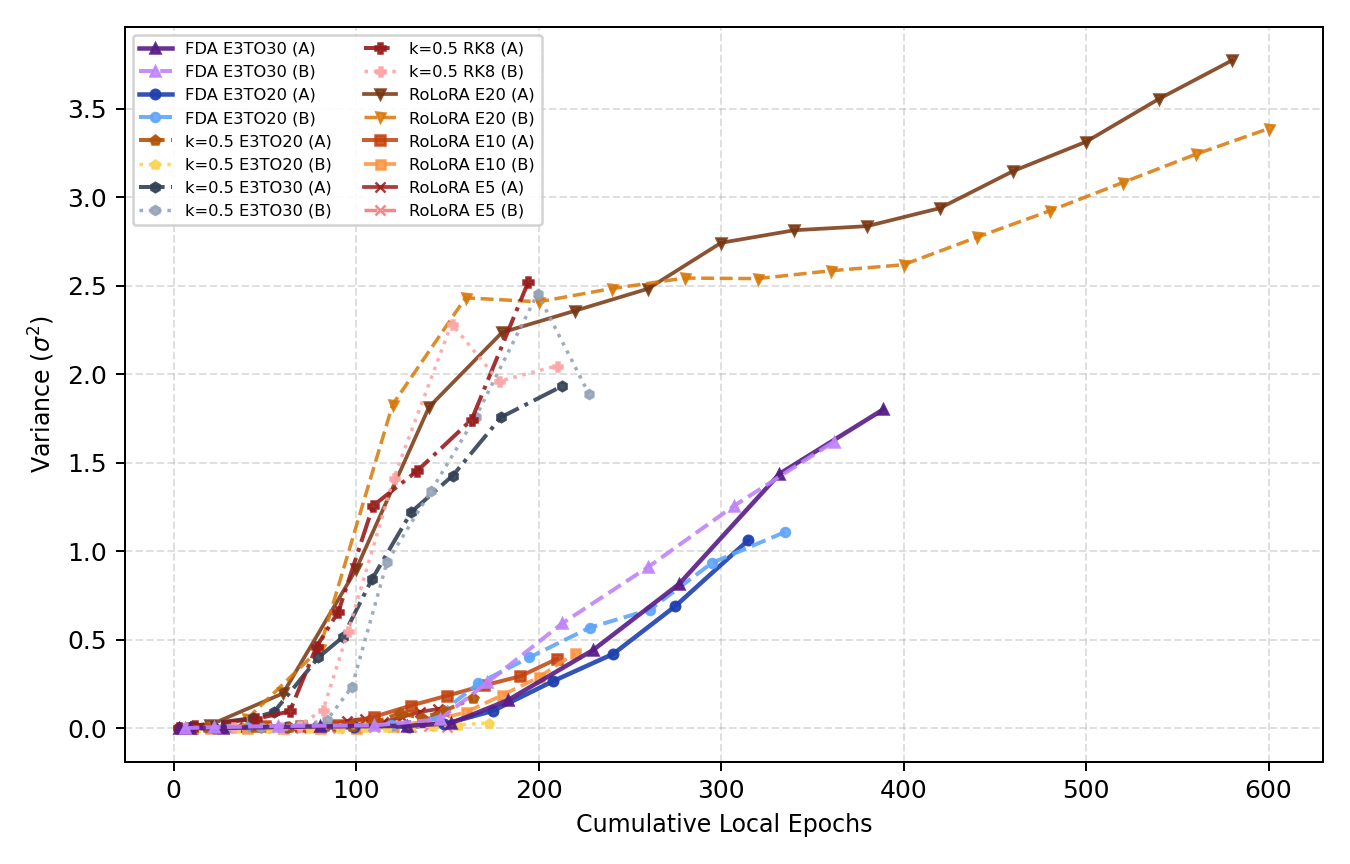
\includegraphics[width=\textwidth,height=4.9cm,keepaspectratio]{figures/telemetry/12_SST2_C50_R30_LR0.1_6_variance_vs_epoch.png}
            \vspace{2pt}
            \par{\footnotesize \textbf{(f)} Variance vs.\ Cumulative Local Epochs}
        \end{minipage}

        \vspace{0.6em}
        \caption{Multi-panel optimization telemetry on SST-2 ($C=50, R_{\max}=30, \eta_c=0.1, \alpha=1000.0$) under expanded cohort scale $C=50$.}
        \label{fig:telemetry_sst2_c50_iid}
    \end{minipage}%
    }
\end{figure}

\clearpage

% ==============================================================================
% SECTION 5.3: BENCHMARK SUITE 2: STATISTICAL HETEROGENEITY
% ==============================================================================
\section{Benchmark Suite 2: Statistical Heterogeneity}
\label{sec:eval_non_iid}

While homogeneous settings demonstrate baseline efficiency, practical federated networks are defined by severe statistical data heterogeneity. To rigorously evaluate the closed-loop resilience of our framework under real-world stress, we investigate severe non-IID conditions modeled via Dirichlet label distribution skew with concentration parameter $\alpha = 0.5$. Adopting $\alpha = 0.5$ directly follows the non-IID benchmarking protocol of RoLoRA~\cite{chen2025robust} and established federated learning literature~\cite{hsu2019measuring, zhu2021federated}, representing an acute label distribution skew where individual clients hold heavily biased class proportions.

Table~\ref{tab:non_iid_detailed_benchmarks} compiles the complete empirical evaluation across all four GLUE sequence classification benchmarks under Dirichlet label skew ($\alpha=0.5$). The table presents all evaluated fixed-budget RoLoRA baselines alongside FDA-RoLoRA across controller horizon ratios $k \in \{0.5, 1.0\}$ and extended horizons ($e_{\max}=40$), explicitly reporting factor-decomposed local epoch allocations ($\bar{e}_A$ and $\bar{e}_B$).

% Auto-generated by FDA-RoLoRA analysis/thesis_final_audit/generate_thesis_tables.py
% Based on code repo commit: 1c2bf55
% Strict data integrity audit: per-seed metrics from raw CSVs in results/round_metrics/
% Do not edit manually.

\begin{table}[htbp]
\centering
\small
\resizebox{\textwidth}{!}{
\begin{tabular}{|l|l|l|c|c|c|c|c|c|c|}
\hline
\textbf{Task} & \textbf{Cohort} & \textbf{Methodology} & \textbf{Final Acc. (\%)} & \textbf{Peak Acc. (\%)} & \textbf{Rounds ($R$)} & \textbf{Total MB} & \textbf{Mean $\bar{e}$} & \textbf{Mean $\bar{e}_A$} & \textbf{Mean $\bar{e}_B$} \\
\hline
\multirow{8}{*}{\textbf{MNLI}} 
& \multirow{5}{*}{$C=20$} 
& FDA-RoLoRA E1TO40 (k=0.5) & $73.70 \pm 0.34$ & $74.12 \pm 0.93$ & $34.5 \pm 0.7$ & $161.7\,\text{MB}$ & $19.06$ & $18.82$ & $19.29$ \\
& & FDA-RoLoRA E1TO20 (k=0.5) & $72.48 \pm 0.14$ & $73.25 \pm 1.19$ & $41.0 \pm 7.1$ & $192.2\,\text{MB}$ & $10.07$ & $9.96$ & $10.18$ \\
& & FDA-RoLoRA E1TO20 (k=1.0) & $73.71 \pm 0.77$ & $\mathbf{74.47 \pm 0.11}$ & $38.0 \pm 4.2$ & $178.1\,\text{MB}$ & $17.49$ & $17.19$ & $17.76$ \\
& & RoLoRA E20 & $68.87 \pm 6.46$ & $73.31 \pm 0.18$ & $\mathbf{24.0 \pm 5.7}$ & $\mathbf{112.5\,\text{MB}}$ & $20.00$ & $20.00$ & $20.00$ \\
& & RoLoRA E10 & $\mathbf{74.11 \pm 0.31}$ & $74.24 \pm 0.12$ & $50.0$ & $234.4\,\text{MB}$ & $10.00$ & $10.00$ & $10.00$ \\
\cline{2-10}
& \multirow{3}{*}{$C=50$} 
& FDA-RoLoRA E1TO20 (k=1.0) & $51.46 \pm 8.46$ & $54.95 \pm 3.53$ & $\mathbf{22.5 \pm 2.1}$ & $\mathbf{263.7\,\text{MB}}$ & $15.63$ & $15.03$ & $16.20$ \\
& & FDA-RoLoRA E1TO20 (k=0.5) & $55.23 \pm 2.11$ & $55.56 \pm 1.65$ & $30.0$ & $351.6\,\text{MB}$ & $10.13$ & $9.47$ & $10.80$ \\
& & RoLoRA E10 & $\mathbf{56.22 \pm 7.40}$ & $\mathbf{56.55 \pm 6.94}$ & $30.0$ & $351.6\,\text{MB}$ & $10.00$ & $10.00$ & $10.00$ \\
\hline
\multirow{9}{*}{\textbf{QNLI}} 
& \multirow{6}{*}{$C=20$} 
& FDA-RoLoRA E1TO40 (k=1.0) & $76.27 \pm 7.78$ & $83.20 \pm 0.18$ & $\mathbf{15.0 \pm 4.2}$ & $\mathbf{70.3\,\text{MB}}$ & $29.83$ & $30.14$ & $29.53$ \\
& & FDA-RoLoRA E1TO40 (k=0.5) & $79.12 \pm 6.72$ & $83.48 \pm 0.94$ & $24.0 \pm 8.5$ & $112.5\,\text{MB}$ & $20.36$ & $21.24$ & $19.47$ \\
& & FDA-RoLoRA E1TO20 (k=1.0) & $81.88 \pm 2.90$ & $\mathbf{84.22 \pm 0.41}$ & $26.5 \pm 7.8$ & $124.2\,\text{MB}$ & $16.73$ & $16.63$ & $16.81$ \\
& & FDA-RoLoRA E1TO20 (k=0.5) & $74.03 \pm 13.98$ & $82.64 \pm 2.63$ & $34.0 \pm 5.7$ & $159.4\,\text{MB}$ & $10.54$ & $10.81$ & $10.27$ \\
& & RoLoRA E20 & $\mathbf{82.97 \pm 0.50}$ & $83.22 \pm 0.14$ & $19.0 \pm 2.8$ & $89.1\,\text{MB}$ & $20.00$ & $20.00$ & $20.00$ \\
& & RoLoRA E10 & $81.10 \pm 4.31$ & $83.50 \pm 1.67$ & $33.0 \pm 1.4$ & $154.7\,\text{MB}$ & $10.00$ & $10.00$ & $10.00$ \\
\cline{2-10}
& \multirow{3}{*}{$C=50$} 
& FDA-RoLoRA E1TO20 (k=1.0) & $49.51 \pm 0.08$ & $73.52 \pm 4.31$ & $\mathbf{13.0}$ & $\mathbf{152.3\,\text{MB}}$ & $13.04$ & $13.17$ & $12.93$ \\
& & FDA-RoLoRA E1TO20 (k=0.5) & $50.13 \pm 0.94$ & $\mathbf{75.69 \pm 1.66}$ & $30.0$ & $351.6\,\text{MB}$ & $10.48$ & $9.83$ & $11.13$ \\
& & RoLoRA E10 & $\mathbf{58.45 \pm 12.71}$ & $74.61 \pm 10.15$ & $30.0$ & $351.6\,\text{MB}$ & $10.00$ & $10.00$ & $10.00$ \\
\hline
\multirow{6}{*}{\textbf{QQP}} 
& \multirow{3}{*}{$C=20$} 
& FDA-RoLoRA E1TO20 (k=1.0) & $64.52 \pm 18.23$ & $\mathbf{77.88 \pm 0.66}$ & $14.0 \pm 2.8$ & $65.6\,\text{MB}$ & $15.70$ & $15.77$ & $15.62$ \\
& & FDA-RoLoRA E1TO20 (k=0.5) & $48.32 \pm 12.63$ & $73.58 \pm 1.56$ & $\mathbf{12.0 \pm 4.2}$ & $\mathbf{56.2\,\text{MB}}$ & $10.87$ & $11.79$ & $10.10$ \\
& & RoLoRA E10 & $\mathbf{76.76 \pm 3.41}$ & $77.69 \pm 2.18$ & $16.5 \pm 0.7$ & $77.3\,\text{MB}$ & $10.00$ & $10.00$ & $10.00$ \\
\cline{2-10}
& \multirow{3}{*}{$C=50$} 
& FDA-RoLoRA E1TO20 (k=1.0) & $57.45 \pm 11.29$ & $74.55 \pm 1.30$ & $\mathbf{15.5 \pm 3.5}$ & $\mathbf{181.6\,\text{MB}}$ & $14.26$ & $13.83$ & $14.63$ \\
& & FDA-RoLoRA E1TO20 (k=0.5) & $53.46 \pm 19.74$ & $72.71 \pm 3.23$ & $\mathbf{15.5 \pm 4.9}$ & $\mathbf{181.6\,\text{MB}}$ & $9.18$ & $8.89$ & $9.48$ \\
& & RoLoRA E10 & $\mathbf{69.28 \pm 8.14}$ & $\mathbf{74.71 \pm 1.63}$ & $22.5 \pm 2.1$ & $263.7\,\text{MB}$ & $10.00$ & $10.00$ & $10.00$ \\
\hline
\multirow{6}{*}{\textbf{SST-2}} 
& \multirow{3}{*}{$C=20$} 
& FDA-RoLoRA E1TO20 (k=1.0) & $69.72 \pm 29.19$ & $\mathbf{89.91 \pm 0.81}$ & $\mathbf{14.0}$ & $\mathbf{39.4\,\text{MB}}$ & $14.43$ & $14.57$ & $14.29$ \\
& & FDA-RoLoRA E1TO20 (k=0.5) & $79.36 \pm 16.38$ & $89.39 \pm 2.19$ & $16.0 \pm 2.8$ & $45.0\,\text{MB}$ & $9.69$ & $10.32$ & $9.06$ \\
& & RoLoRA E10 & $\mathbf{89.62 \pm 1.87}$ & $89.62 \pm 1.87$ & $25.0$ & $70.3\,\text{MB}$ & $10.00$ & $10.00$ & $10.00$ \\
\cline{2-10}
& \multirow{3}{*}{$C=50$} 
& FDA-RoLoRA E1TO20 (k=1.0) & $\mathbf{81.36 \pm 9.97}$ & $\mathbf{85.95 \pm 5.60}$ & $\mathbf{20.0}$ & $\mathbf{140.6\,\text{MB}}$ & $14.57$ & $14.60$ & $14.55$ \\
& & FDA-RoLoRA E1TO20 (k=0.5) & $66.46 \pm 24.57$ & $67.37 \pm 23.27$ & $\mathbf{20.0}$ & $\mathbf{140.6\,\text{MB}}$ & $8.70$ & $8.40$ & $9.00$ \\
& & RoLoRA E10 & $53.33 \pm 3.08$ & $59.00 \pm 11.11$ & $\mathbf{20.0}$ & $\mathbf{140.6\,\text{MB}}$ & $10.00$ & $10.00$ & $10.00$ \\
\hline
\end{tabular}
}
\caption{Detailed Telemetry Across All Non-IID Configurations ($\alpha=0.5$): RoLoRA vs.\ FDA-RoLoRA across GLUE benchmarks under Dirichlet label skew.}
\label{tab:non_iid_detailed_benchmarks}
\end{table}

\paragraph{MNLI: Asymmetric Factor Allocation \& Post-Peak Collapse.}
On 3-class sentence-pair inference under acute Dirichlet label skew ($\alpha=0.5, C=20, R_{\max}=50$), Figure~\ref{fig:telemetry_mnli_non_iid} illustrates optimization dynamics across all six telemetry panels. Under static schedules ($E=20$), forcing clients through unconstrained local training drives updates into conflicting subspaces: validation accuracy (Panel a) peaks early at $73.31\%$ and then suffers catastrophic post-peak collapse down to $68.09\%$. In contrast, FDA-RoLoRA ($k=1.0$) dynamically monitors coordinate variance, achieving a superior peak accuracy of $\mathbf{74.47\%}$ and stopping after 41 and 35 rounds (seeds 42 and 43) at final accuracies of $73.17\%$ and $74.25\%$. At those same rounds, RoLoRA $E=10$ had reached only $70.23\%$ and $71.86\%$, and it needed 47 and 50 rounds to match FDA-RoLoRA's final accuracy. FDA-RoLoRA therefore reaches the same accuracy in roughly 15--30\% fewer rounds ($178.1\,\text{MB}$ vs.\ $234.4\,\text{MB}$ on average), while executing about $1.75\times$ more local epochs per round ($\bar{e}=17.49$ vs.\ 10). 

Crucially, local epoch telemetry (Panel c) and decoupled threshold trajectories (Panel d) reveal the mechanistic basis of this stability: factor matrix $B$ safely accommodates deeper local training ($\bar{e}_B = 17.76$) under an expanded threshold $\theta_B$, whereas down-projection factor $A$ encounters sharper gradient drift, prompting threshold $\theta_A$ to enforce earlier synchronization ($\bar{e}_A = 17.19$). Subspace coordinate variance (Panel e) surges by over $2\times$ compared to IID regimes ($\bar{\nu} \approx 6.5\text{--}8.0$), reflecting severe inter-client gradient conflict.
\begin{figure}[p]
    \centering
    \makebox[\textwidth][c]{%
    \begin{minipage}{1.06\textwidth}
        \begin{minipage}[b]{0.485\textwidth}
            \centering
            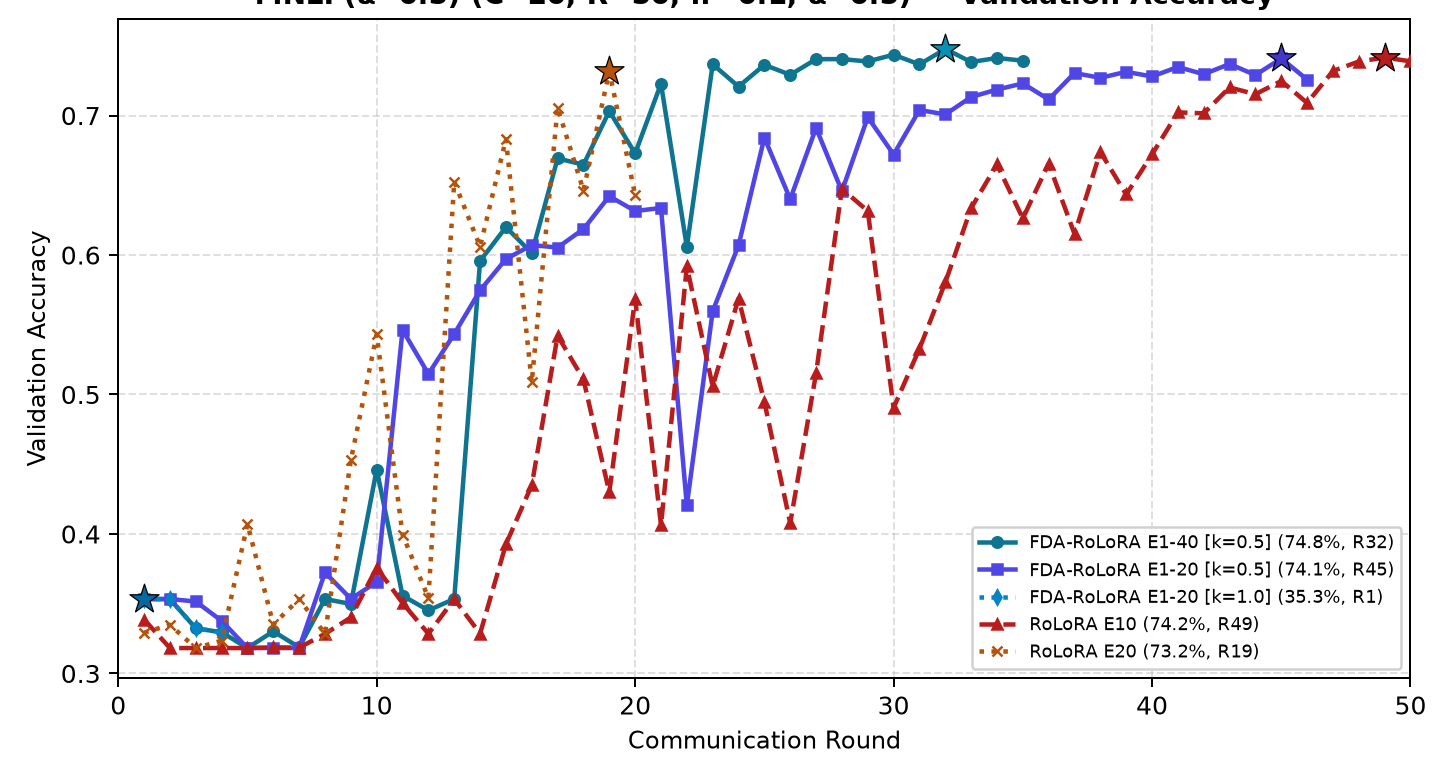
\includegraphics[width=\textwidth,height=4.9cm,keepaspectratio]{figures/telemetry/17_MNLI_C20_R50_LR0.1_A0.5_1_accuracy.png}
            \vspace{2pt}
            \par{\footnotesize \textbf{(a)} Validation Accuracy}
        \end{minipage}\hfill
        \begin{minipage}[b]{0.485\textwidth}
            \centering
            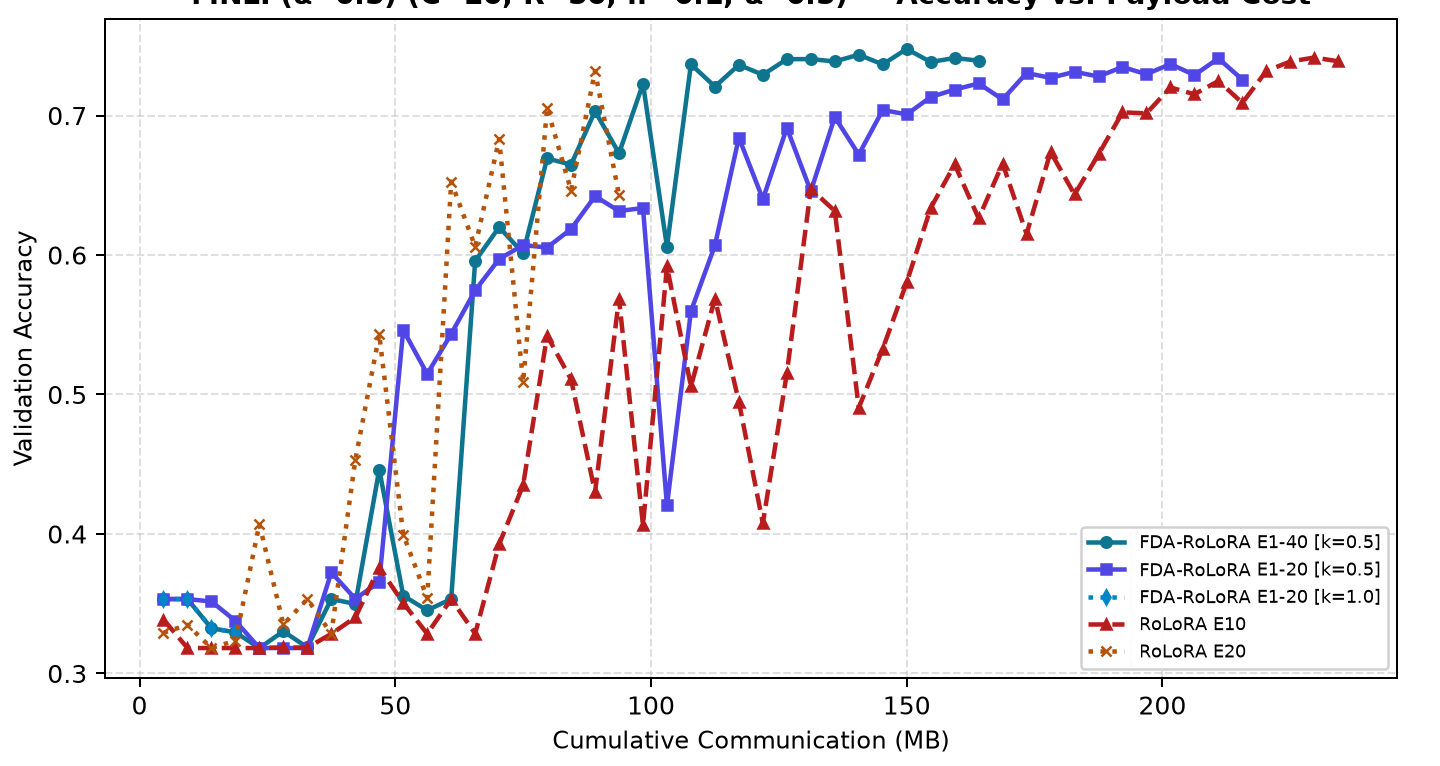
\includegraphics[width=\textwidth,height=4.9cm,keepaspectratio]{figures/telemetry/17_MNLI_C20_R50_LR0.1_A0.5_4_accuracy_vs_cost.png}
            \vspace{2pt}
            \par{\footnotesize \textbf{(b)} Accuracy vs. Communication (MB)}
        \end{minipage}

        \vspace{0.6em}
        \begin{minipage}[b]{0.485\textwidth}
            \centering
            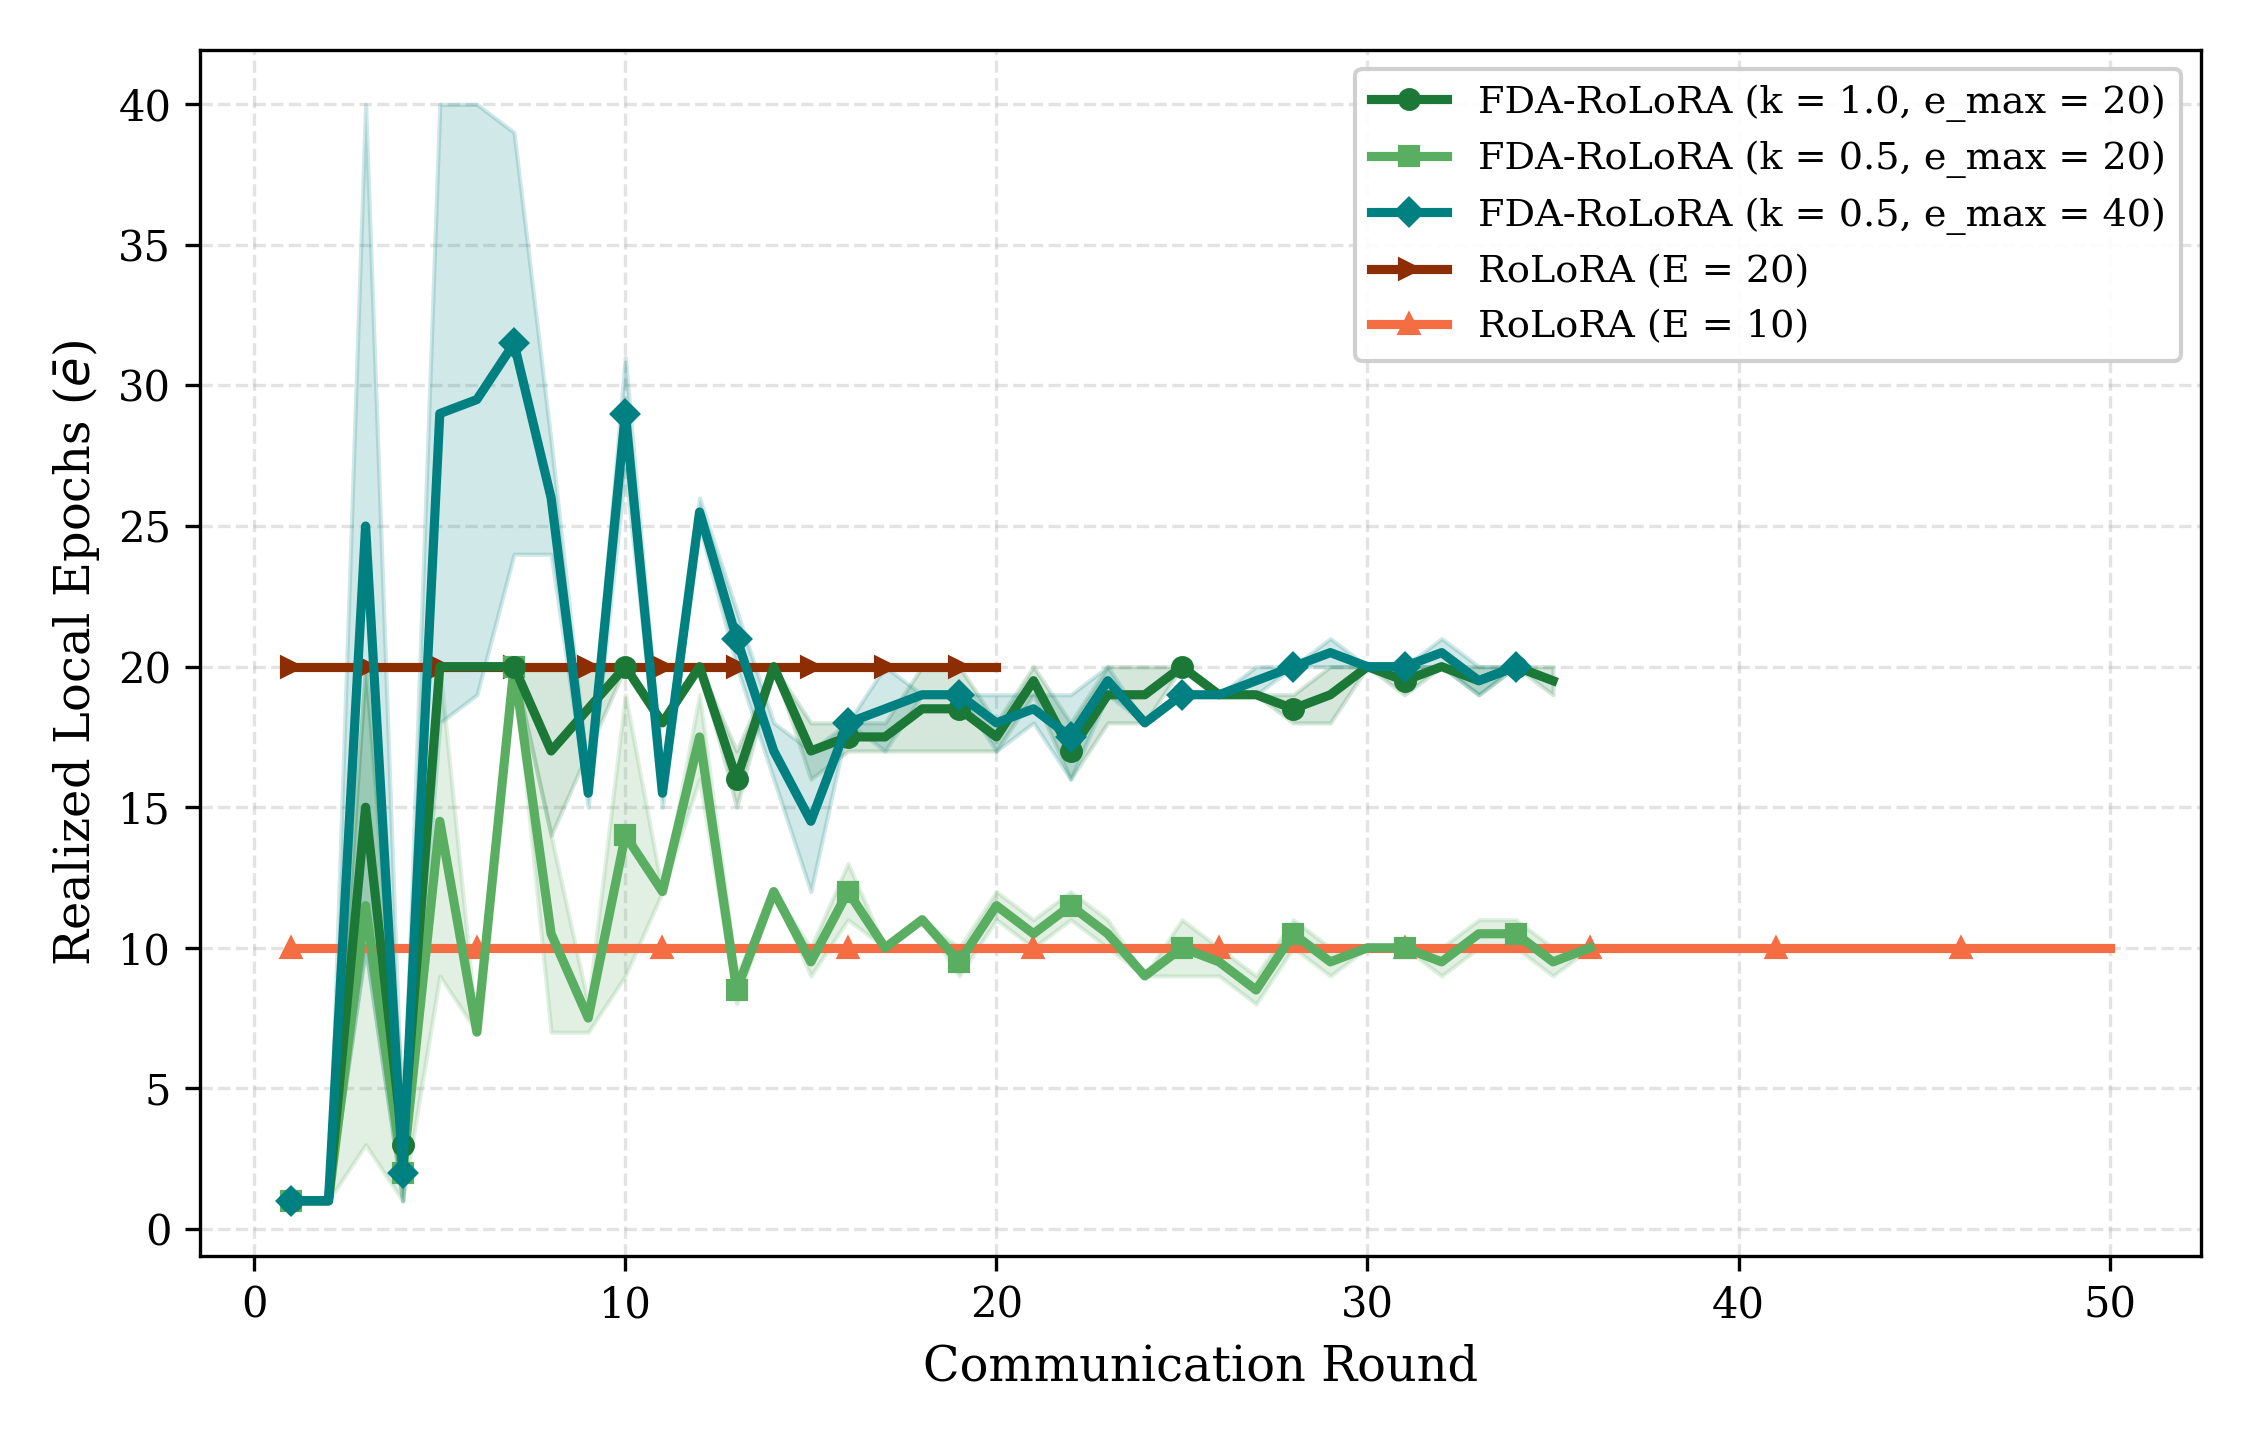
\includegraphics[width=\textwidth,height=4.9cm,keepaspectratio]{figures/telemetry/17_MNLI_C20_R50_LR0.1_A0.5_2_allocated_epochs.png}
            \vspace{2pt}
            \par{\footnotesize \textbf{(c)} Dynamic Local Epochs ($\bar{e}$)}
        \end{minipage}\hfill
        \begin{minipage}[b]{0.485\textwidth}
            \centering
            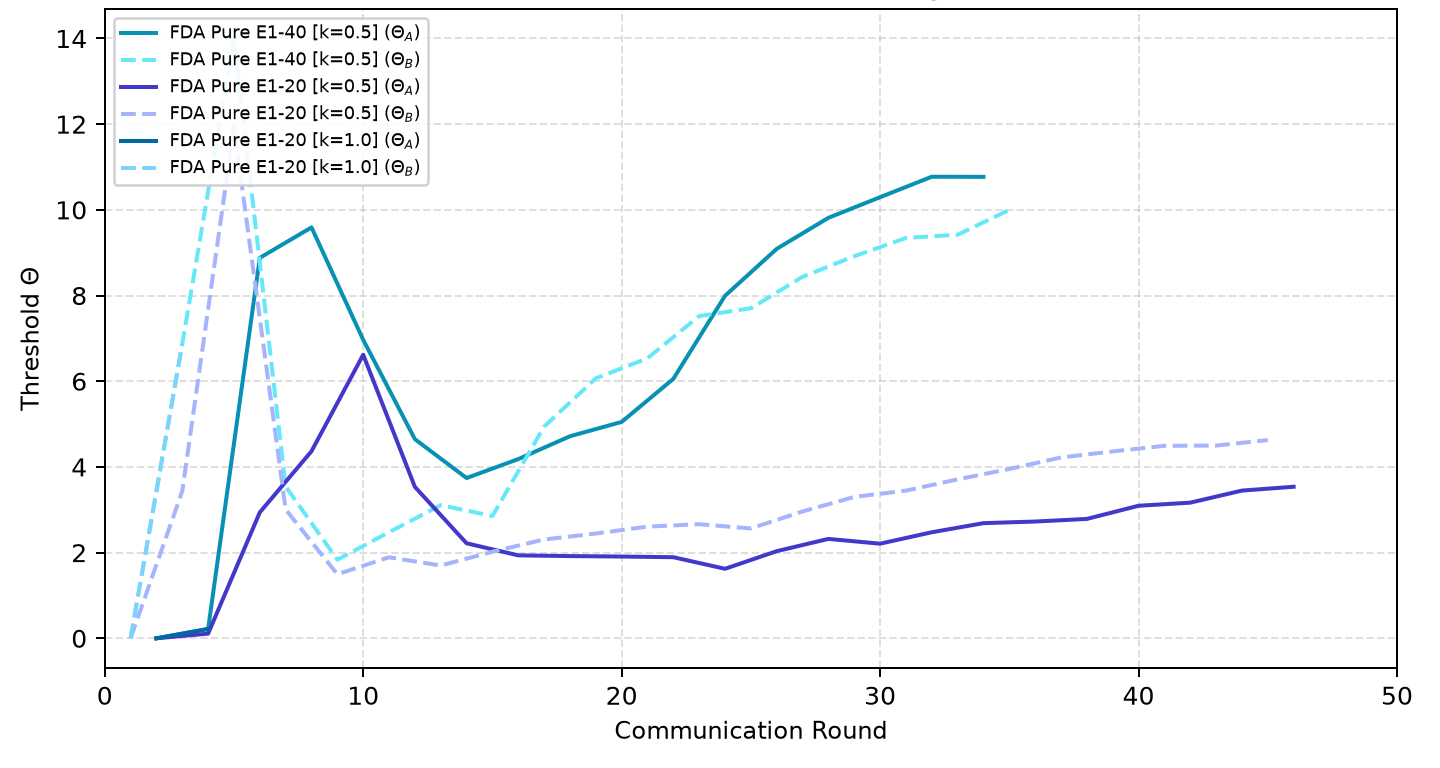
\includegraphics[width=\textwidth,height=4.9cm,keepaspectratio]{figures/telemetry/17_MNLI_C20_R50_LR0.1_A0.5_5_fda_threshold.png}
            \vspace{2pt}
            \par{\footnotesize \textbf{(d)} Factor Thresholds ($\theta_A, \theta_B$)}
        \end{minipage}

        \vspace{0.6em}
        \begin{minipage}[b]{0.485\textwidth}
            \centering
            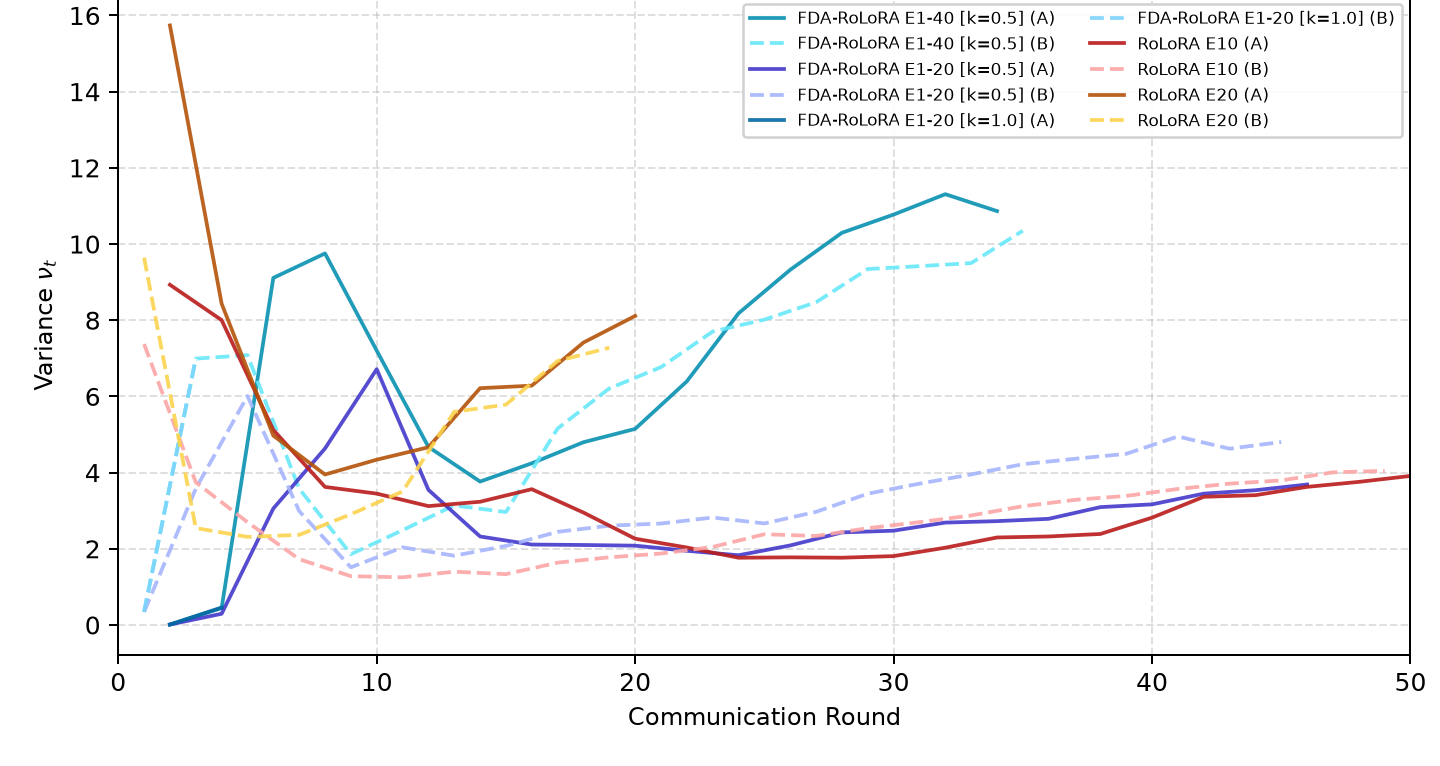
\includegraphics[width=\textwidth,height=4.9cm,keepaspectratio]{figures/telemetry/17_MNLI_C20_R50_LR0.1_A0.5_3_client_variance.png}
            \vspace{2pt}
            \par{\footnotesize \textbf{(e)} Subspace Coordinate Variance}
        \end{minipage}\hfill
        \begin{minipage}[b]{0.485\textwidth}
            \centering
            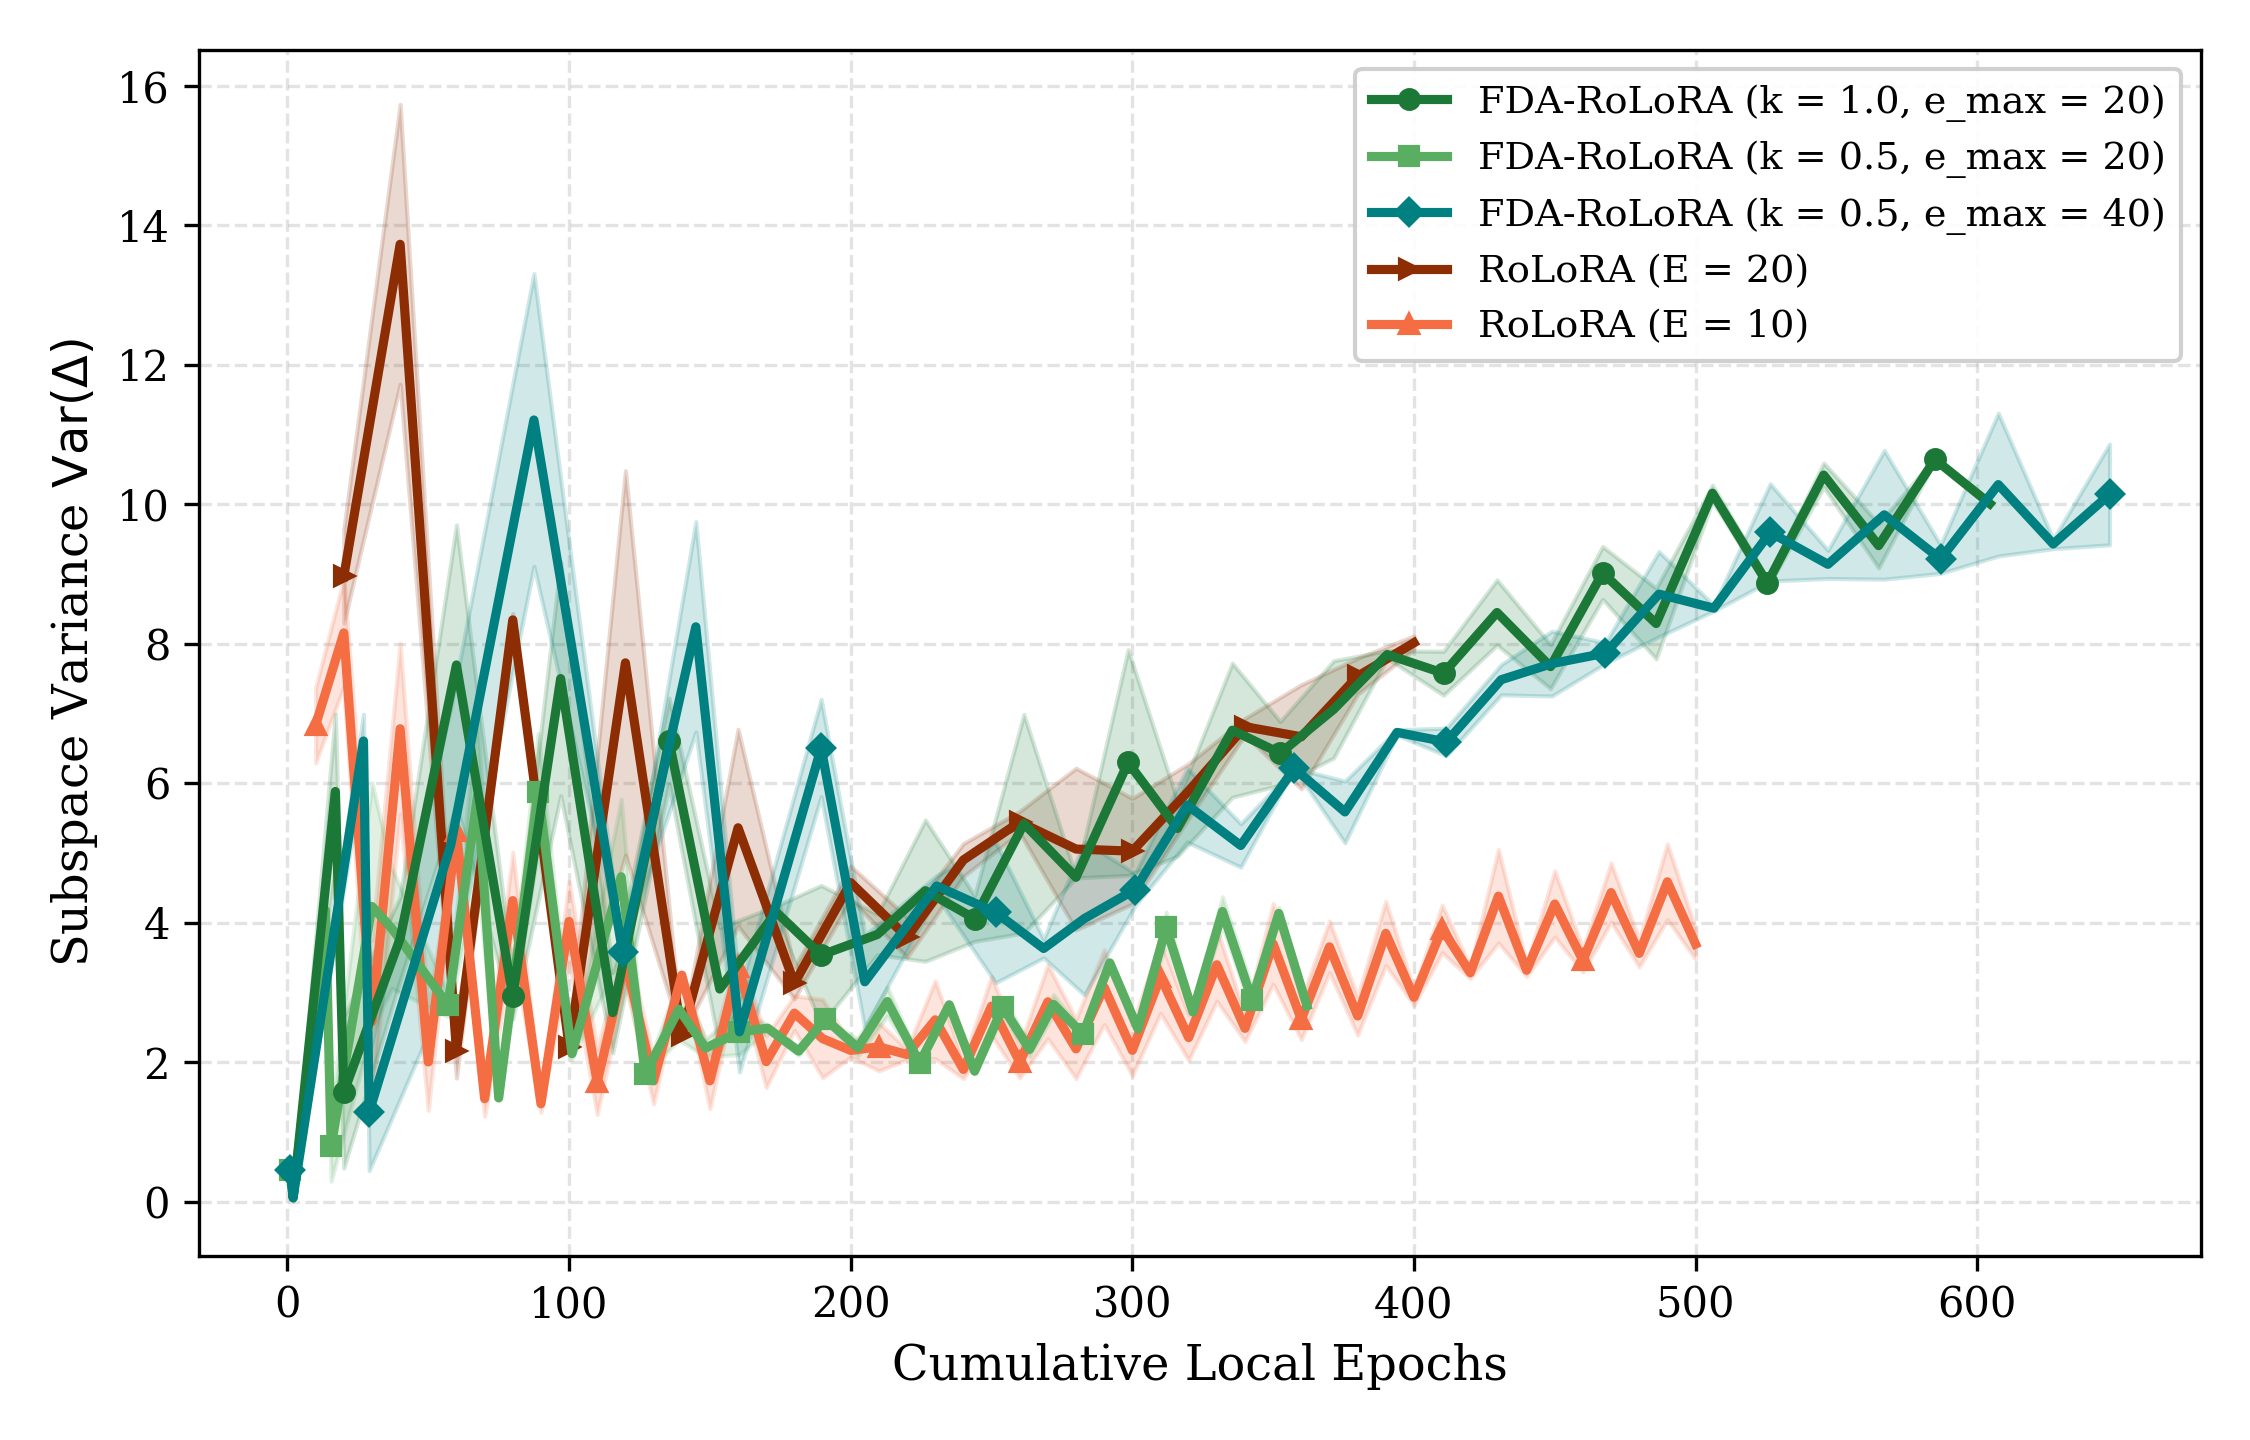
\includegraphics[width=\textwidth,height=4.9cm,keepaspectratio]{figures/telemetry/17_MNLI_C20_R50_LR0.1_A0.5_6_variance_vs_epoch.png}
            \vspace{2pt}
            \par{\footnotesize \textbf{(f)} Variance vs.\ Cumulative Local Epochs}
        \end{minipage}

        \vspace{0.6em}
        \caption{Multi-panel optimization telemetry on MNLI under Dirichlet label skew ($\alpha=0.5, C=20, R_{\max}=50, \eta_c=0.1$) comparing FDA-RoLoRA against static baselines.}
        \label{fig:telemetry_mnli_non_iid}
    \end{minipage}%
    }
\end{figure}

\paragraph{QNLI: Scalability \& Suite-Leading Peak Accuracy.}
Binary question-answering under skew demonstrates the scalability of closed-loop synchronization across the six telemetry dimensions (Figure~\ref{fig:telemetry_qnli_non_iid}). On $C=20$ ($R_{\max}=50$), FDA-RoLoRA ($k=1.0$) attains the highest peak validation accuracy across the entire non-IID benchmark suite ($\mathbf{84.22\%}$, Panel a), dominating the communication-cost curve (Panel b) over static baselines. With an expanded ceiling $e_{\max}=40$, the controller successfully expands local computation to $\bar{e} = 29.83$ epochs (Panel c) while tracking smooth, decoupled factor thresholds $\theta_A$ and $\theta_B$ (Panel d). Drift variance at synchronization (Panel e) stabilizes at $\bar{\nu} \approx 1.79$.

When scaling to $C=50$ clients under acute skew ($R_{\max}=30$), aggressive setpoint scaling ($k=1.0$) over-allocated local epochs in early rounds, precipitating client drift and tripping early stopping at round 13.0 ($152.3\,\text{MB}$, $49.51\%$ accuracy). With midpoint scaling ($k=0.5$), FDA-RoLoRA reaches a peak of $75.69 \pm 1.66\%$ (RoLoRA $E=10$: $74.61 \pm 10.15\%$), but both FDA-RoLoRA variants end near chance level (final $49.51\%$ for $k=1.0$ and $50.13\%$ for $k=0.5$), so no communication saving is claimed for this configuration. The $k=1.0$ runs used a round budget of $R_{\max}=22$.
\begin{figure}[p]
    \centering
    \makebox[\textwidth][c]{%
    \begin{minipage}{1.06\textwidth}
        \begin{minipage}[b]{0.485\textwidth}
            \centering
            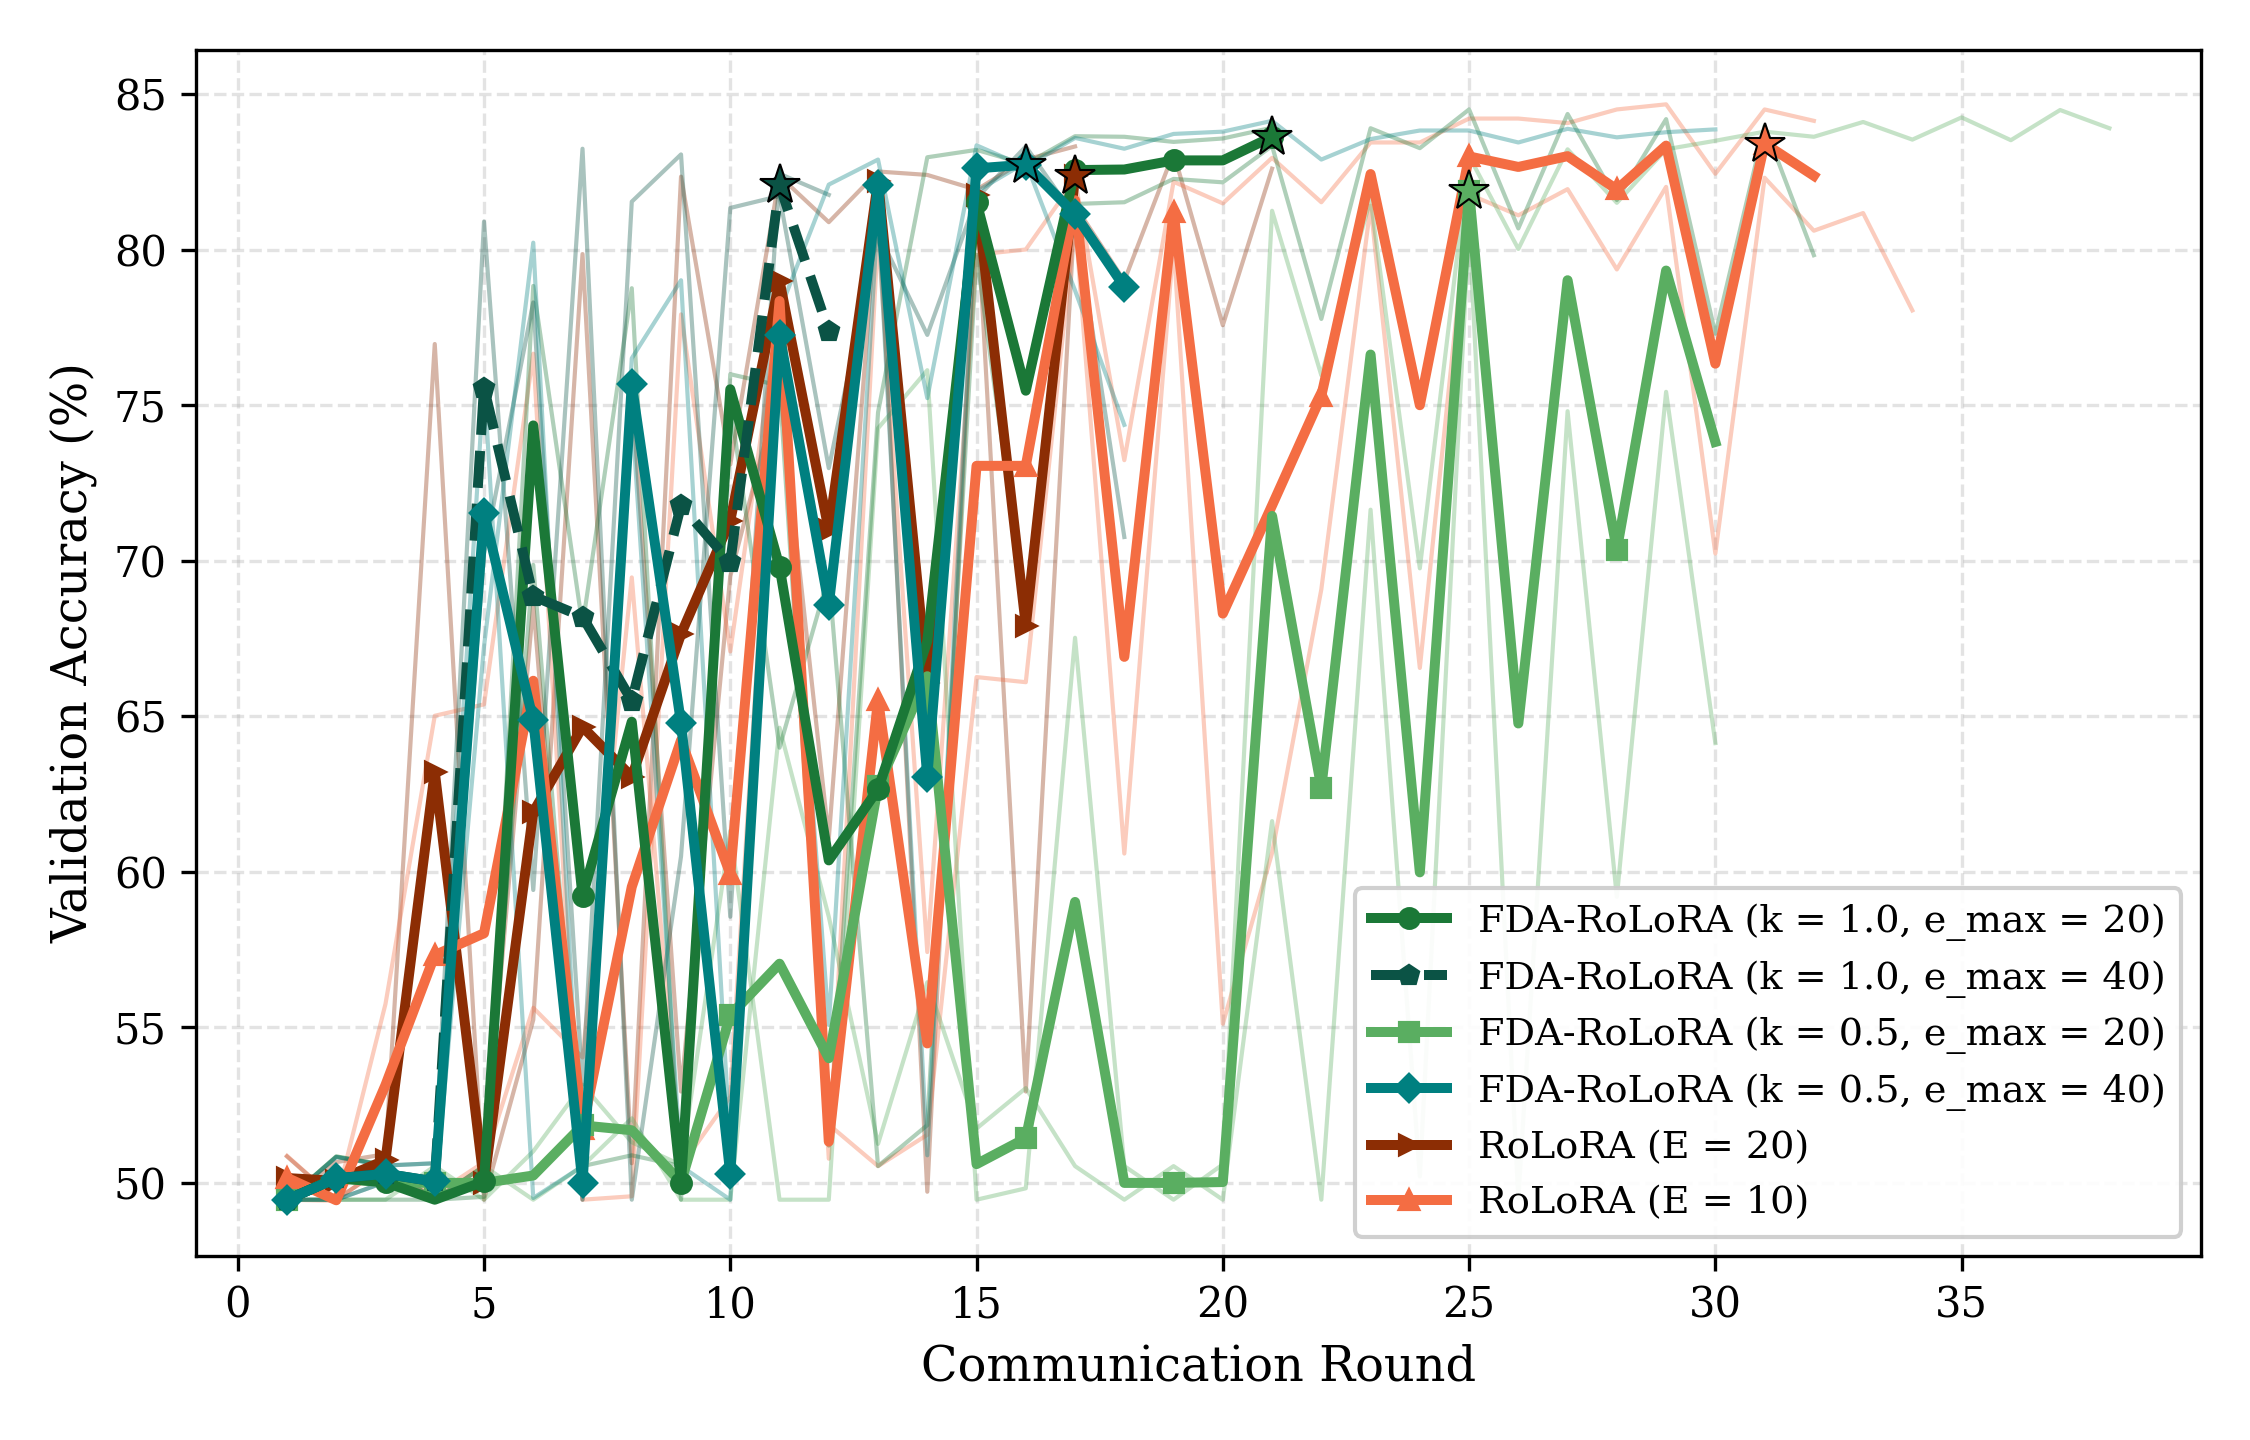
\includegraphics[width=\textwidth,height=4.9cm,keepaspectratio]{figures/telemetry/18_QNLI_C20_R50_LR0.1_A0.5_1_accuracy.png}
            \vspace{2pt}
            \par{\footnotesize \textbf{(a)} Validation Accuracy}
        \end{minipage}\hfill
        \begin{minipage}[b]{0.485\textwidth}
            \centering
            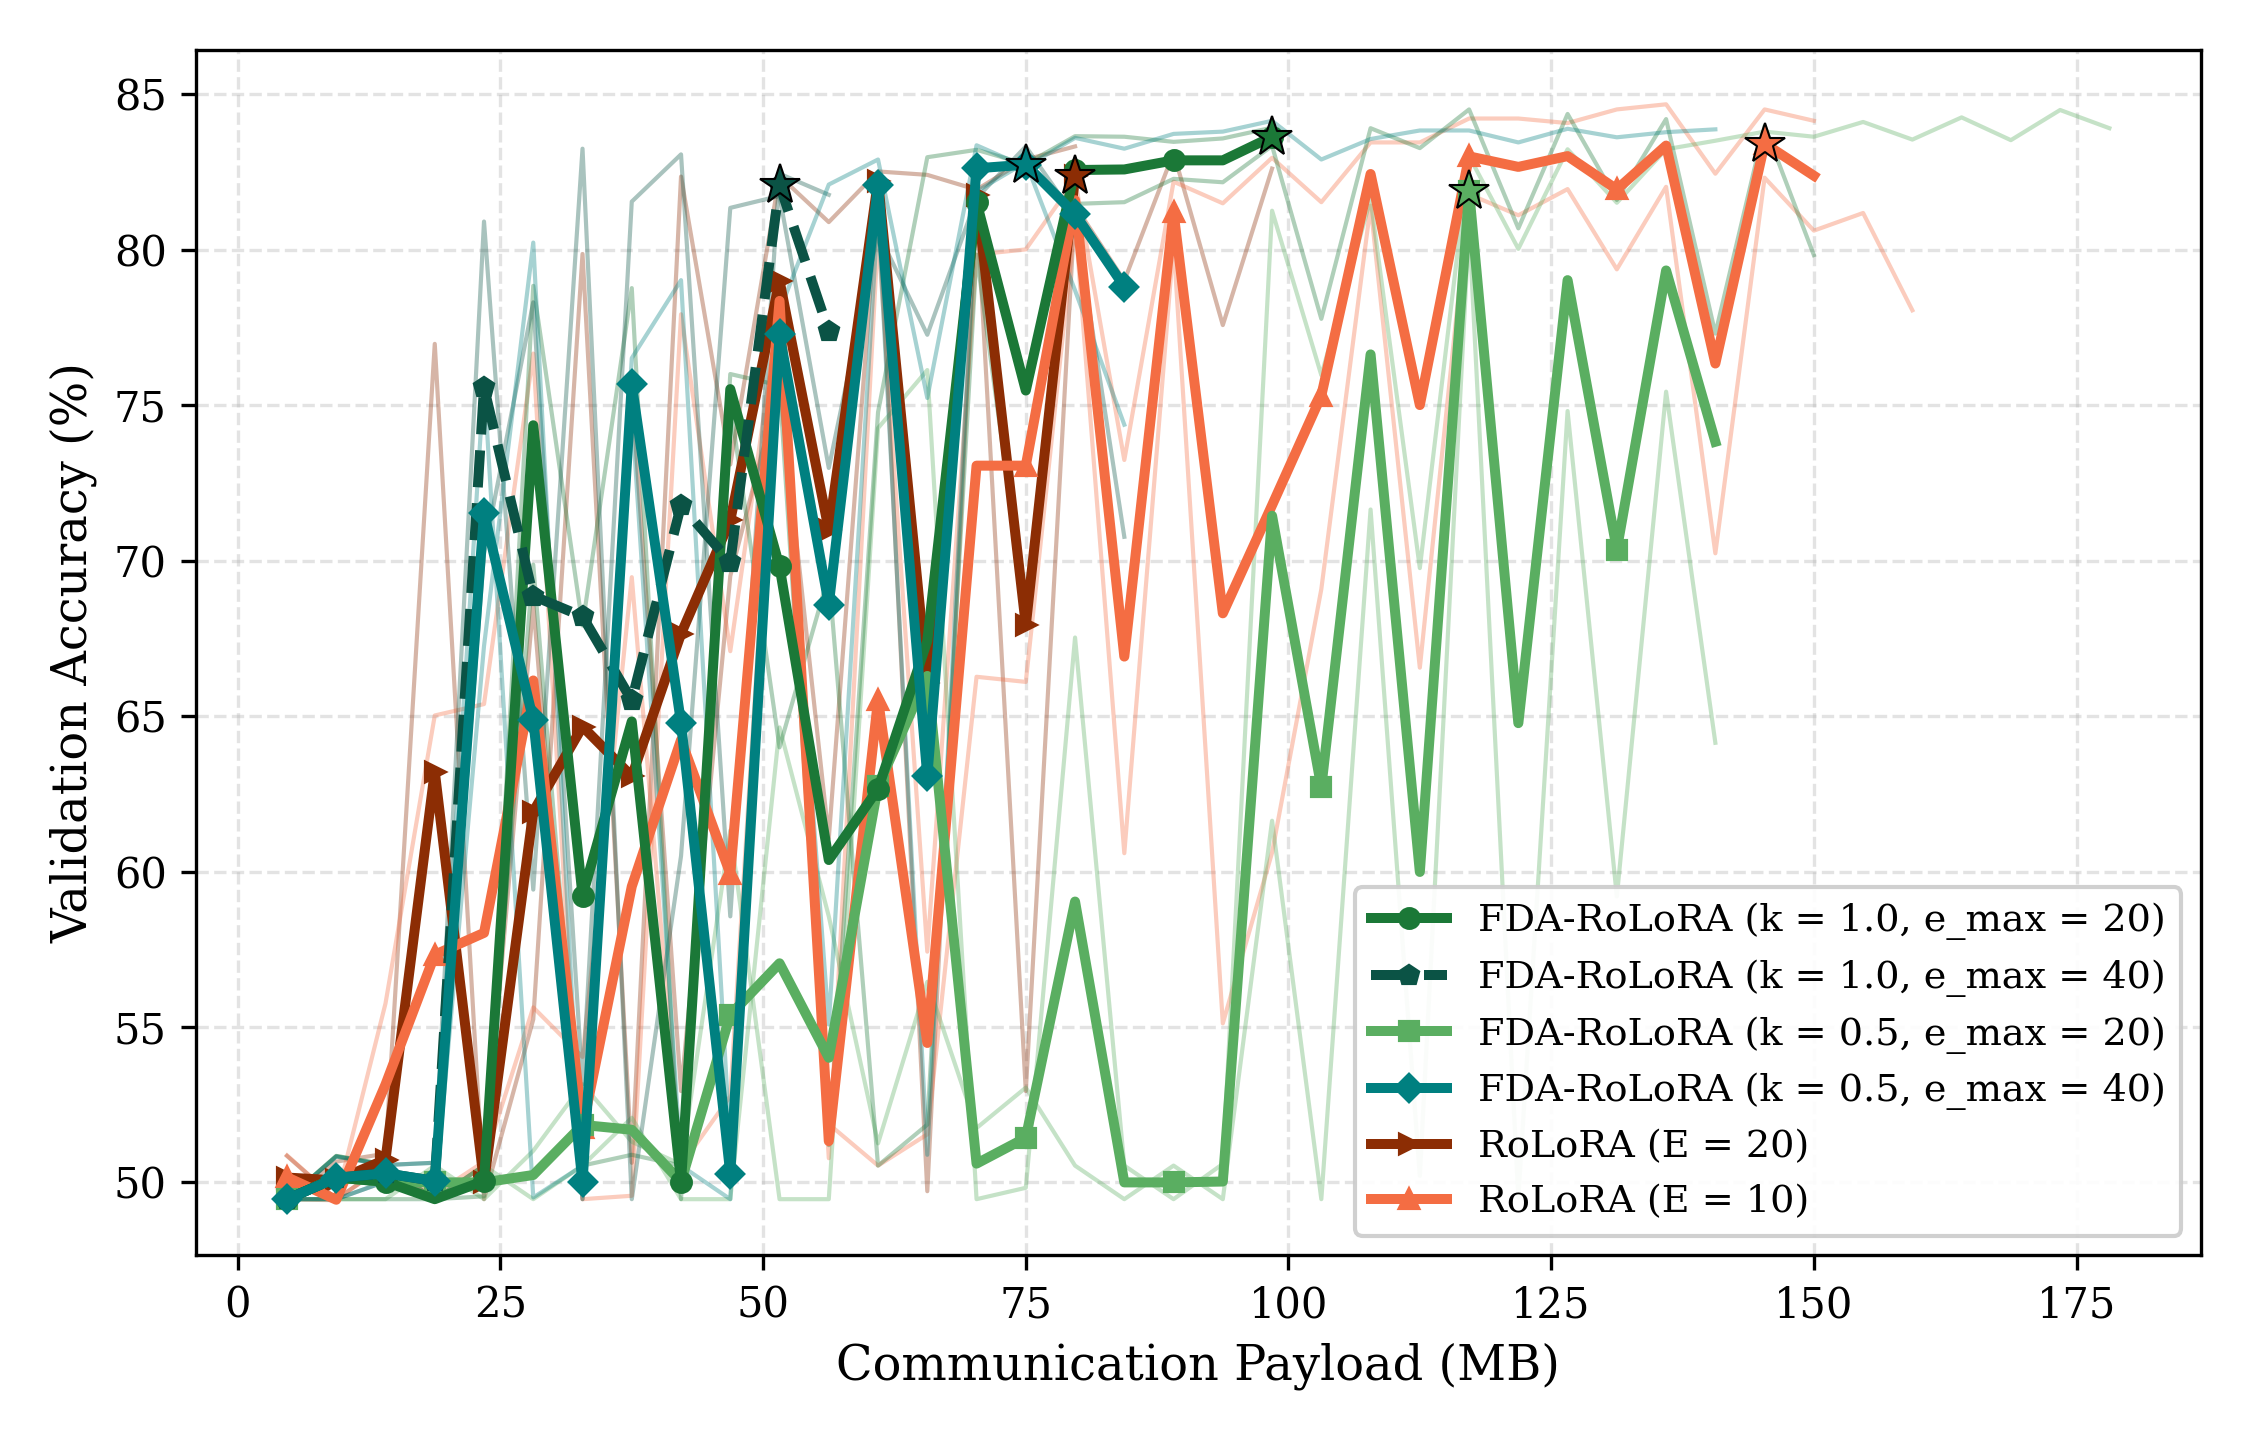
\includegraphics[width=\textwidth,height=4.9cm,keepaspectratio]{figures/telemetry/18_QNLI_C20_R50_LR0.1_A0.5_4_accuracy_vs_cost.png}
            \vspace{2pt}
            \par{\footnotesize \textbf{(b)} Accuracy vs. Communication (MB)}
        \end{minipage}

        \vspace{0.6em}
        \begin{minipage}[b]{0.485\textwidth}
            \centering
            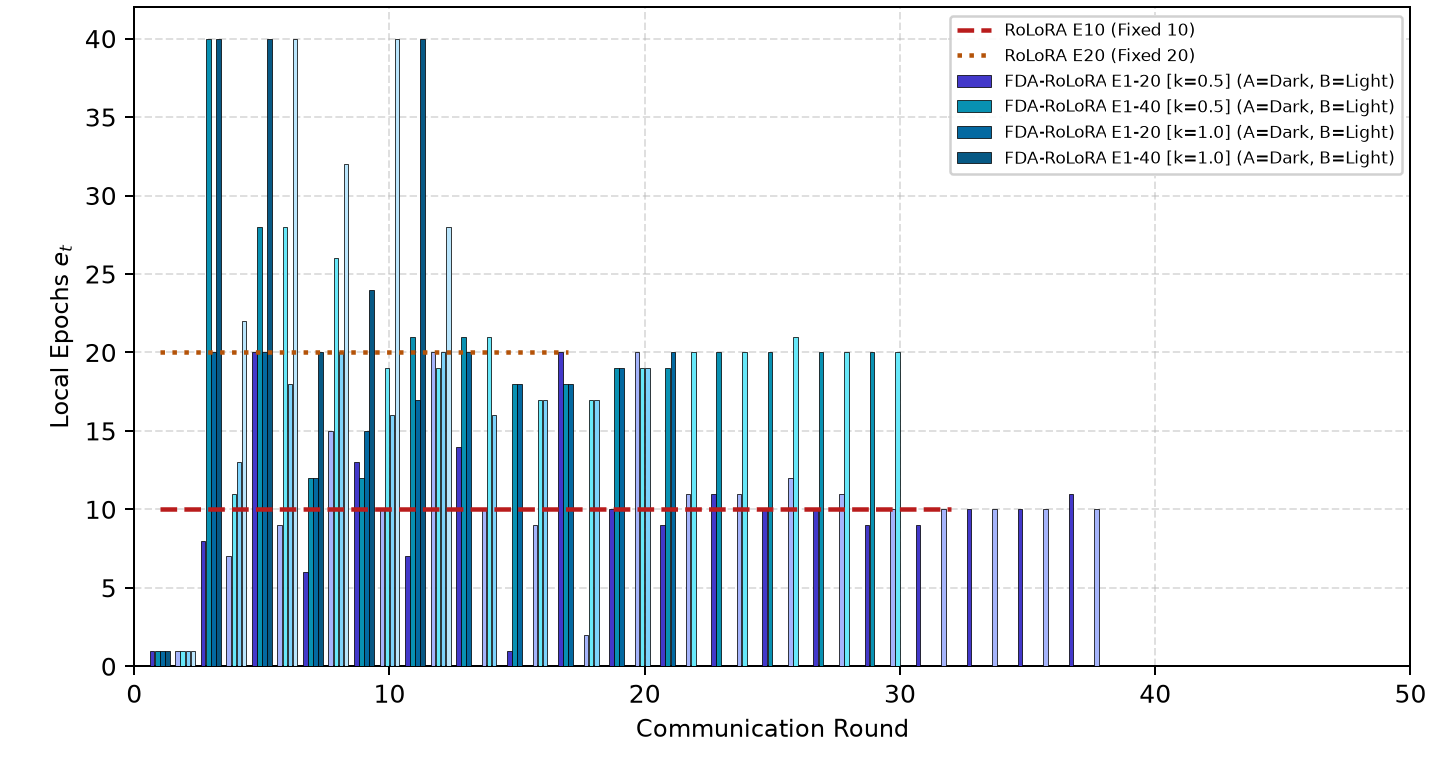
\includegraphics[width=\textwidth,height=4.9cm,keepaspectratio]{figures/telemetry/18_QNLI_C20_R50_LR0.1_A0.5_2_allocated_epochs.png}
            \vspace{2pt}
            \par{\footnotesize \textbf{(c)} Dynamic Local Epochs ($\bar{e}$)}
        \end{minipage}\hfill
        \begin{minipage}[b]{0.485\textwidth}
            \centering
            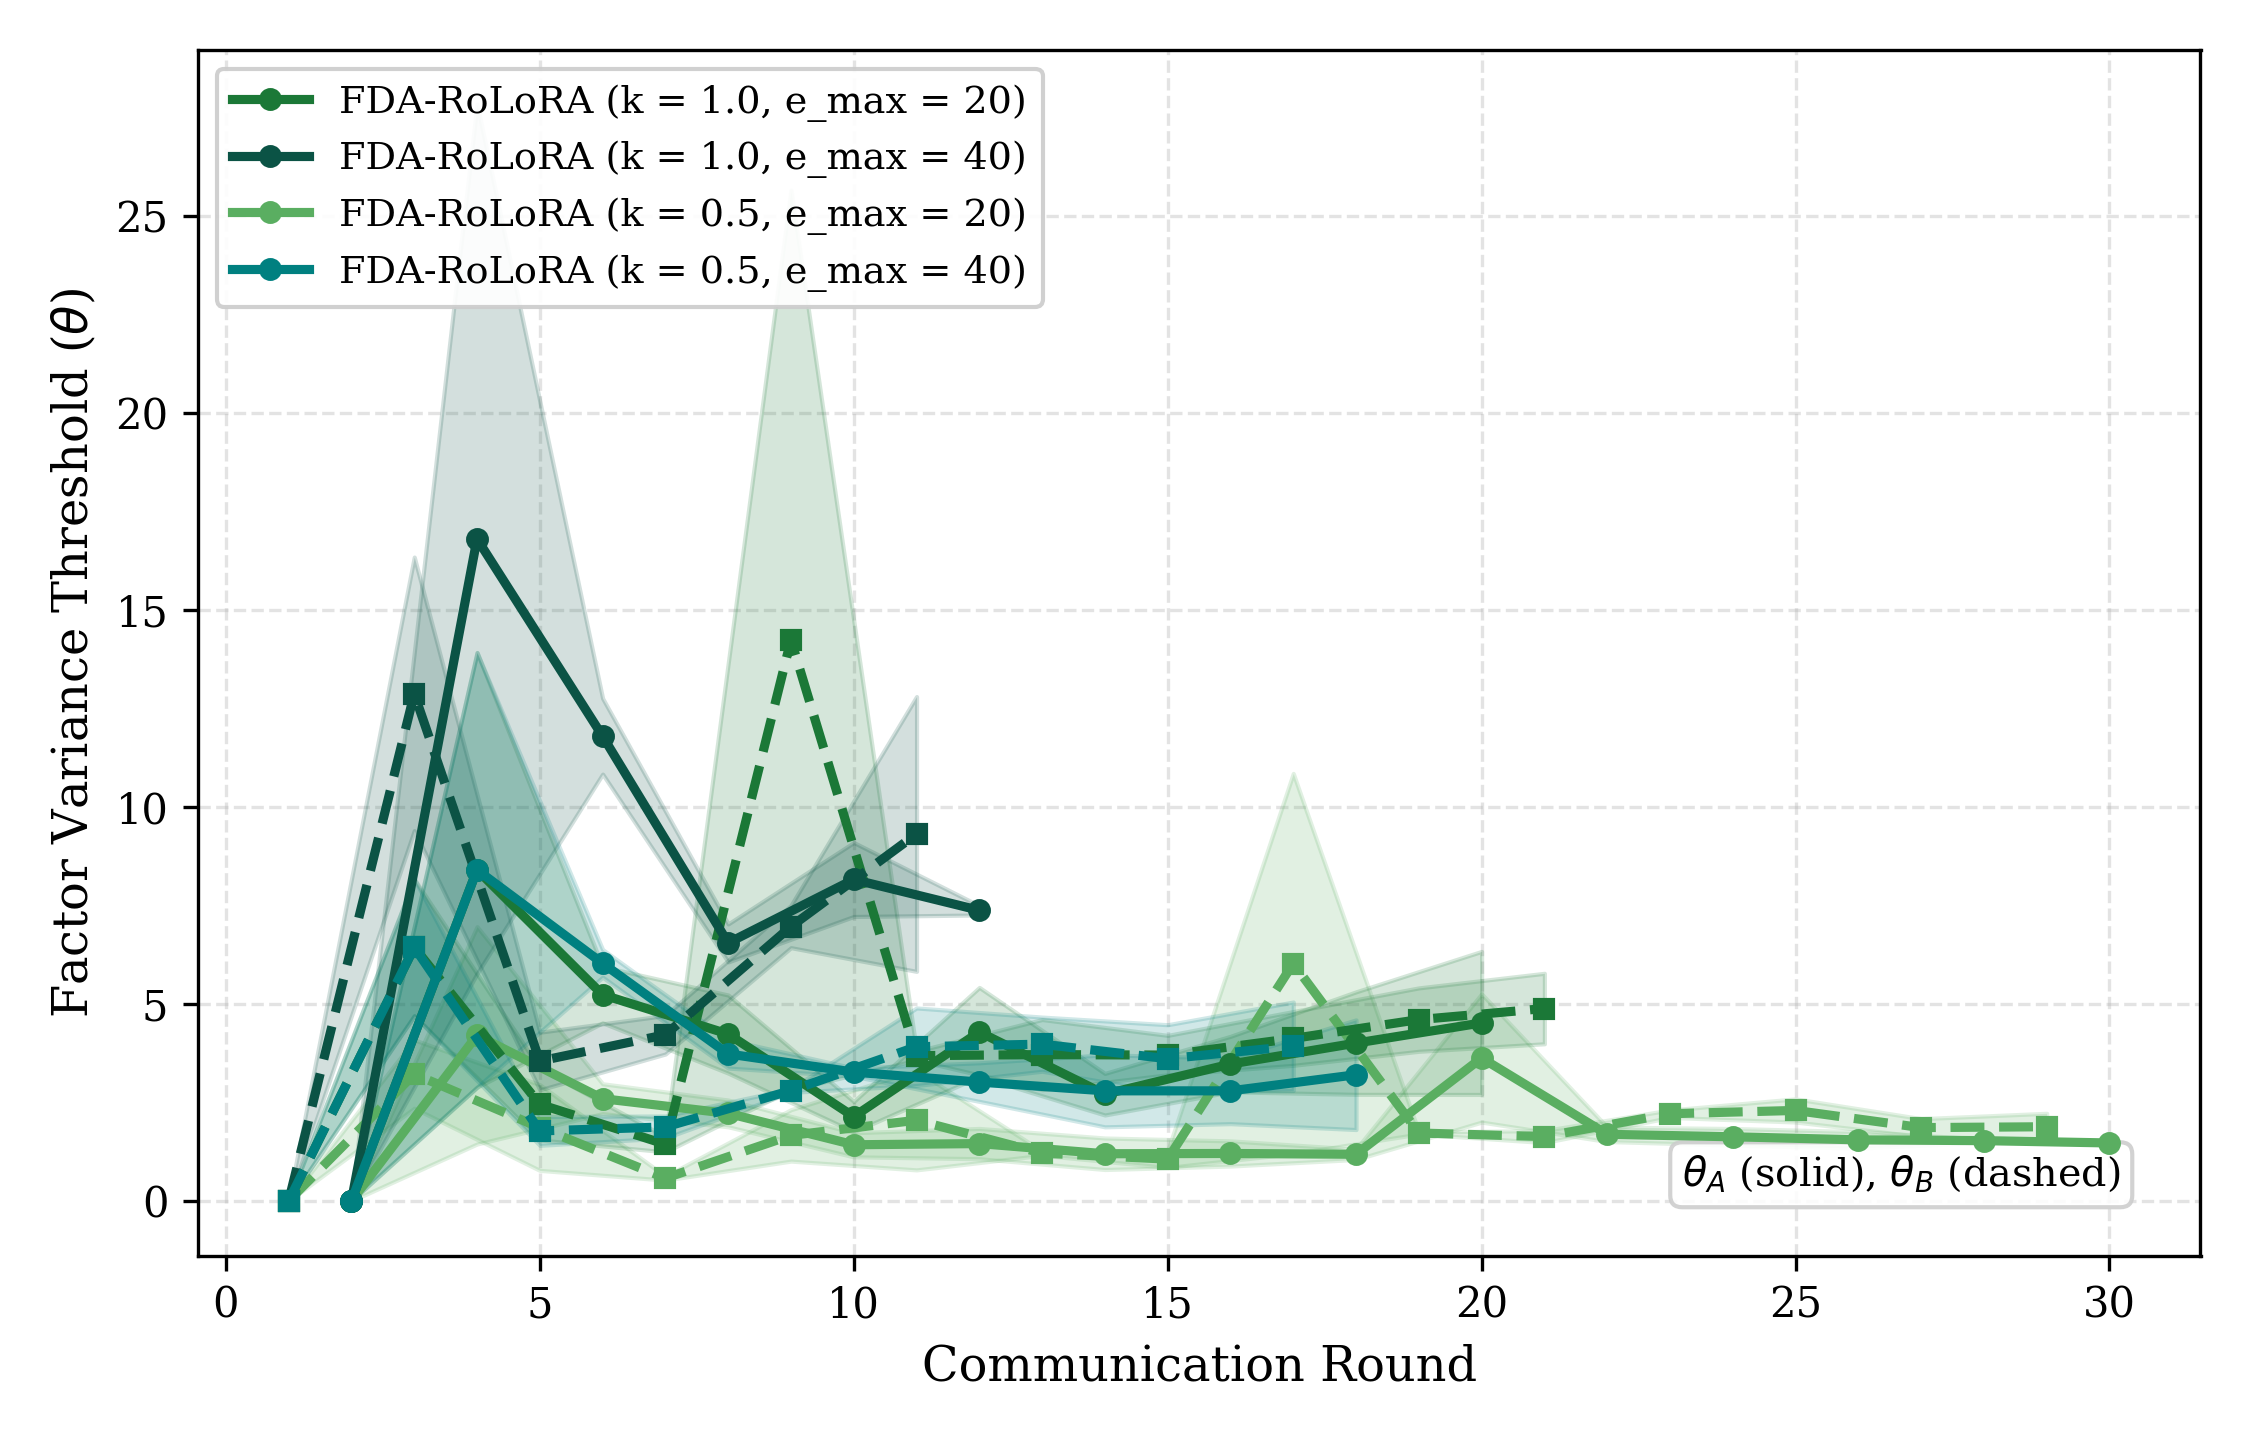
\includegraphics[width=\textwidth,height=4.9cm,keepaspectratio]{figures/telemetry/18_QNLI_C20_R50_LR0.1_A0.5_5_fda_threshold.png}
            \vspace{2pt}
            \par{\footnotesize \textbf{(d)} Factor Thresholds ($\theta_A, \theta_B$)}
        \end{minipage}

        \vspace{0.6em}
        \begin{minipage}[b]{0.485\textwidth}
            \centering
            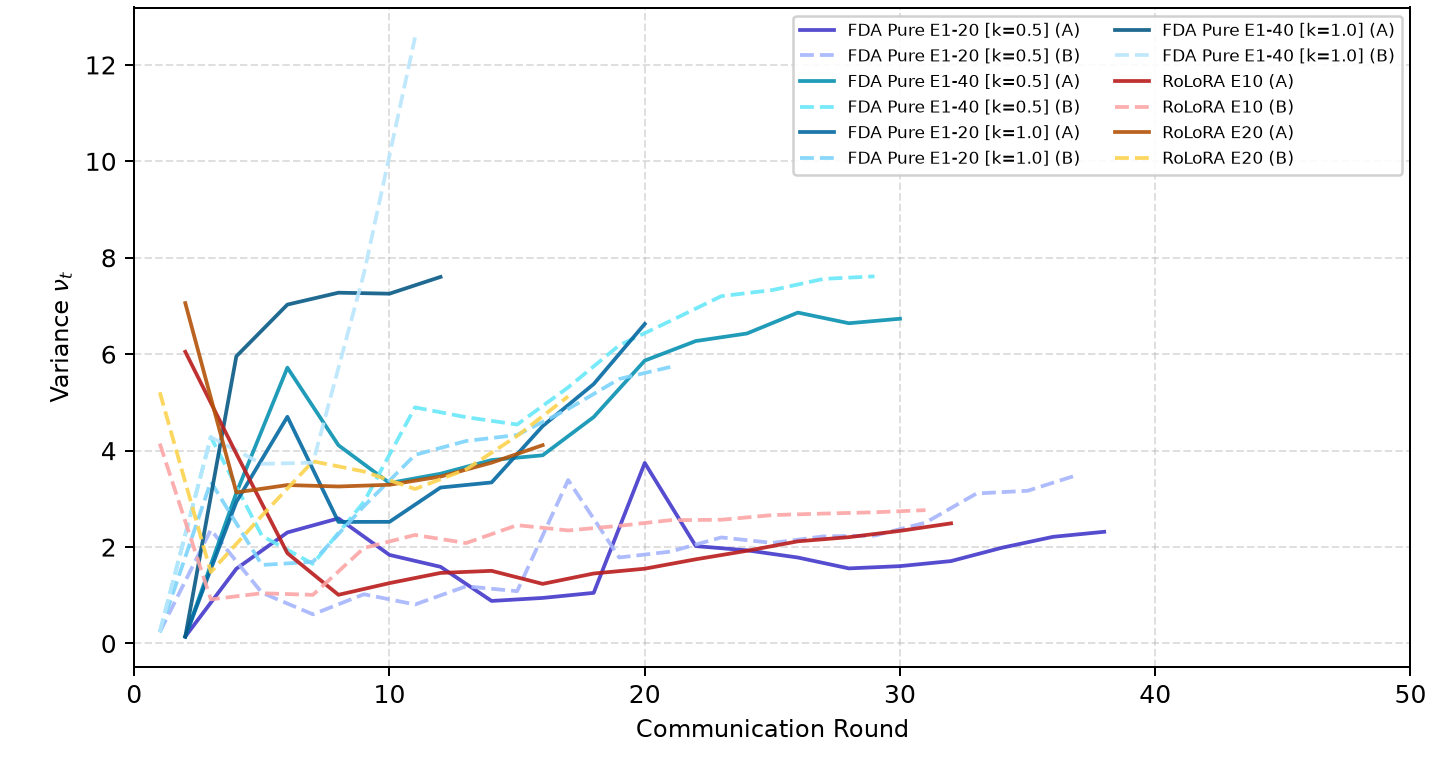
\includegraphics[width=\textwidth,height=4.9cm,keepaspectratio]{figures/telemetry/18_QNLI_C20_R50_LR0.1_A0.5_3_client_variance.png}
            \vspace{2pt}
            \par{\footnotesize \textbf{(e)} Subspace Coordinate Variance}
        \end{minipage}\hfill
        \begin{minipage}[b]{0.485\textwidth}
            \centering
            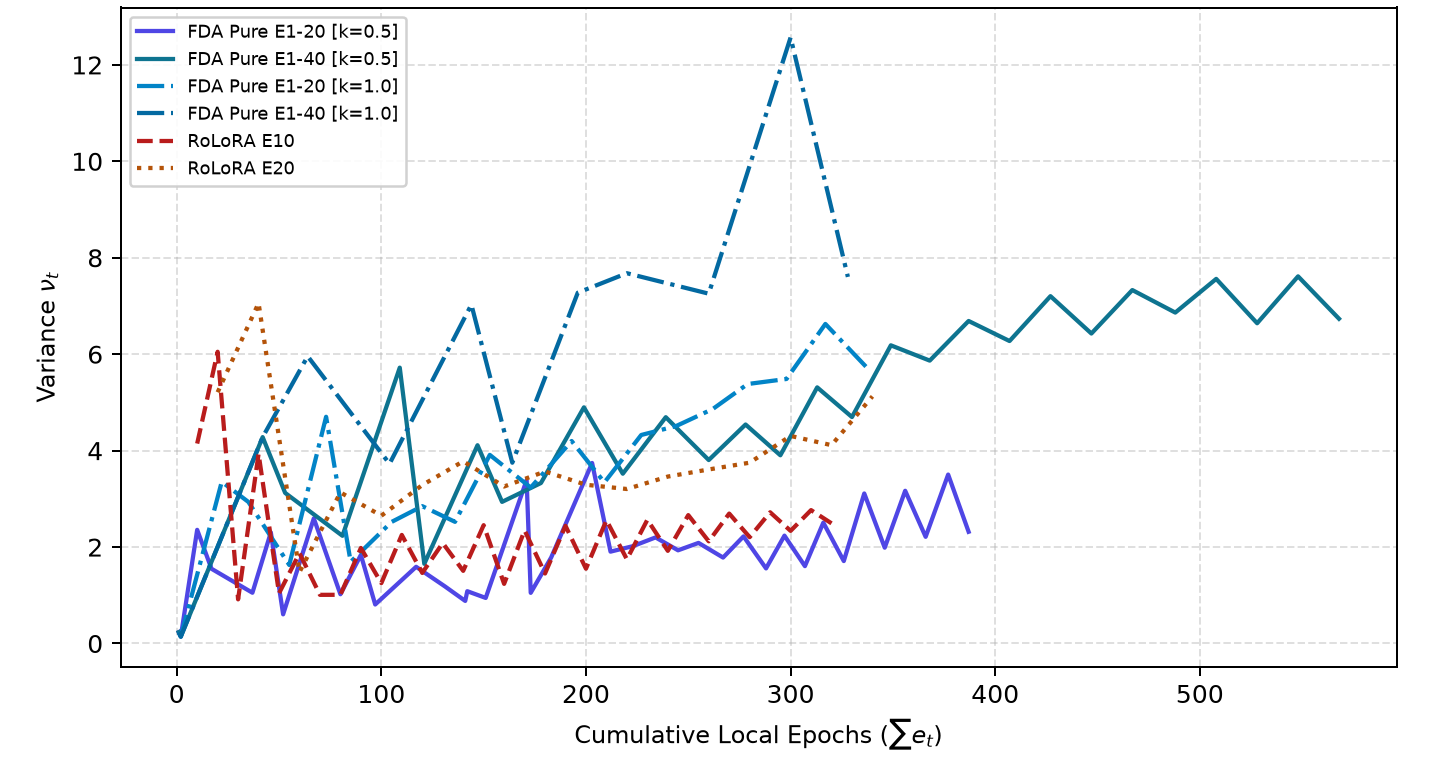
\includegraphics[width=\textwidth,height=4.9cm,keepaspectratio]{figures/telemetry/18_QNLI_C20_R50_LR0.1_A0.5_6_variance_vs_epoch.png}
            \vspace{2pt}
            \par{\footnotesize \textbf{(f)} Variance vs.\ Cumulative Local Epochs}
        \end{minipage}

        \vspace{0.6em}
        \caption{Multi-panel optimization telemetry on QNLI under Dirichlet label skew ($\alpha=0.5, C=20, R_{\max}=50, \eta_c=0.1$) comparing FDA-RoLoRA against static baselines.}
        \label{fig:telemetry_qnli_non_iid}
    \end{minipage}%
    }
\end{figure}

\paragraph{Dynamic Round Synchronization and Realized Epoch Dynamics.}
Figure~\ref{fig:non_iid_epoch_dynamics} visualizes round-by-round realized local epoch allocations on MNLI and QNLI under statistical heterogeneity. When Dirichlet skew causes local client updates to diverge sharply in coordinate space, inter-client drift variance surges by approximately $4.0\times$ (e.g., from $0.448$ to $1.794$ on QNLI). While static baselines execute a constant number of local passes regardless of parameter divergence, FDA-RoLoRA's closed-loop controller constrains local passes within $[e_{\min}, e_{\max}]$ in response to coordinate variance breaches, enforcing earlier server synchronization to mitigate client drift.

\begin{figure}[htbp]
    \centering
    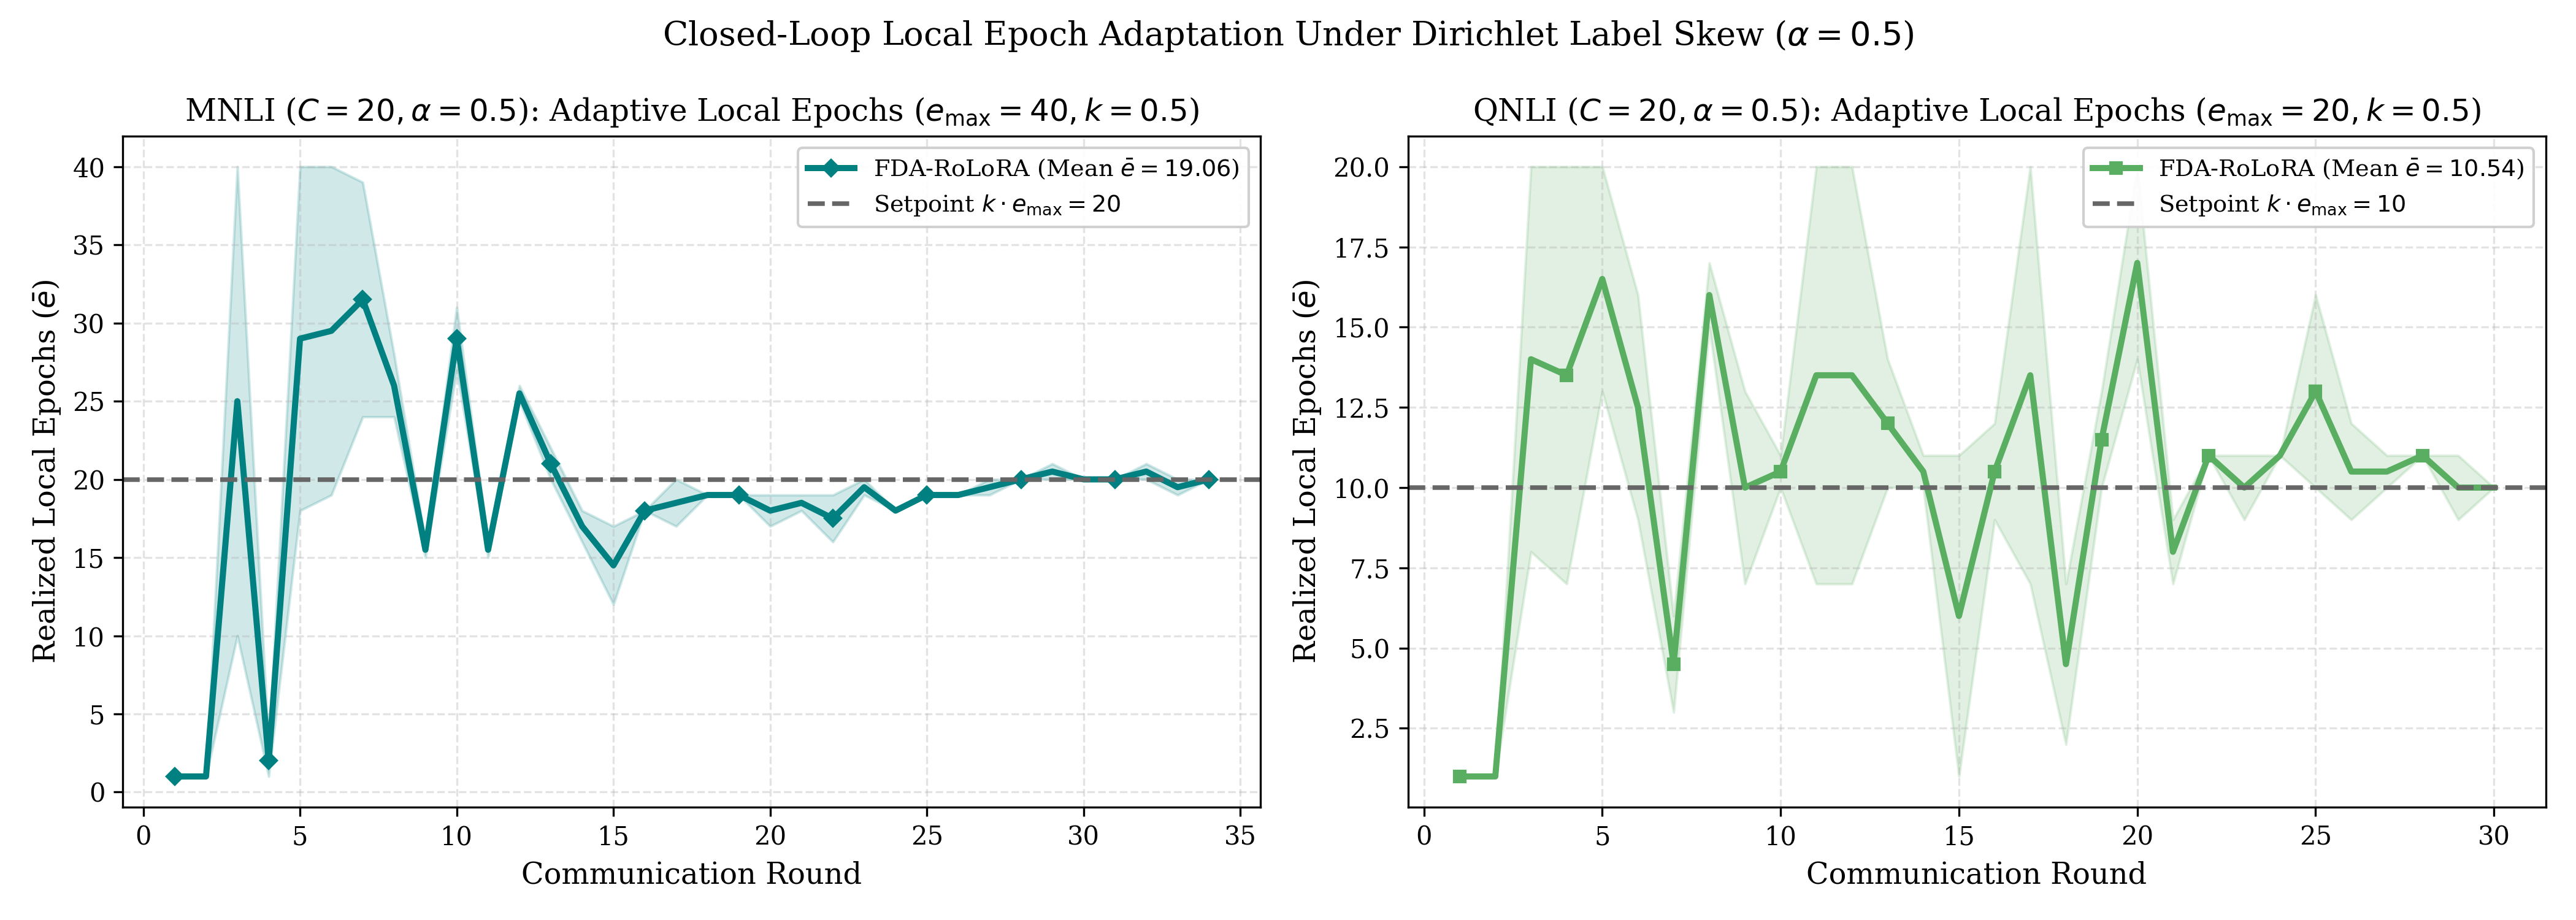
\includegraphics[width=0.95\textwidth]{figures/non_iid_epoch_dynamics.png}
    \caption{Empirical local epoch allocation dynamics under severe statistical heterogeneity (Dirichlet label skew $\alpha=0.5$), illustrating the closed-loop setpoint tracking dynamics of FDA-RoLoRA on MNLI and QNLI under Dirichlet label skew ($\alpha=0.5$).}
    \label{fig:non_iid_epoch_dynamics}
\end{figure}

\paragraph{SST-2 \& QQP: Cross-Task Drift and Anti-Collapse Protection.}
Figure~\ref{fig:non_iid_benchmark_telemetry} provides a focused diagnostic synthesis on MNLI and QNLI of federated fine-tuning under acute Dirichlet label skew ($\alpha=0.5$). The most pronounced empirical difference occurs on SST-2 with 50 clients. Under static $E=10$, RoLoRA did not leave the initial majority-class plateau within the 20-round budget in either seed (final $51.15\%$ and $55.50\%$), remaining trapped at the majority-class baseline ($\sim 50\%$) for the majority of rounds before an isolated surge to $59.00 \pm 11.11\%$ peak accuracy ($53.33 \pm 3.08\%$ final). In contrast, FDA-RoLoRA ($k=1.0$) dynamically navigated the loss landscape to escape the plateau, attaining $\mathbf{85.95 \pm 5.60\%}$ peak accuracy (final $88.42\%$ and $74.31\%$ in the two seeds), with a higher mean local-epoch count ($\bar{e}=14.57$ vs.\ 10), representing a \textbf{+26.95\% absolute improvement in peak accuracy}. On QQP ($C=50$), FDA-RoLoRA stops earlier (15.5 vs.\ 22.5 rounds), but one seed ended at chance level ($49.46\%$), and its mean final accuracy ($57.45\%$) is below RoLoRA $E=10$ ($69.28\%$). The earlier stop is therefore not a saving at equal accuracy.



\begin{figure}[htbp]
    \centering
    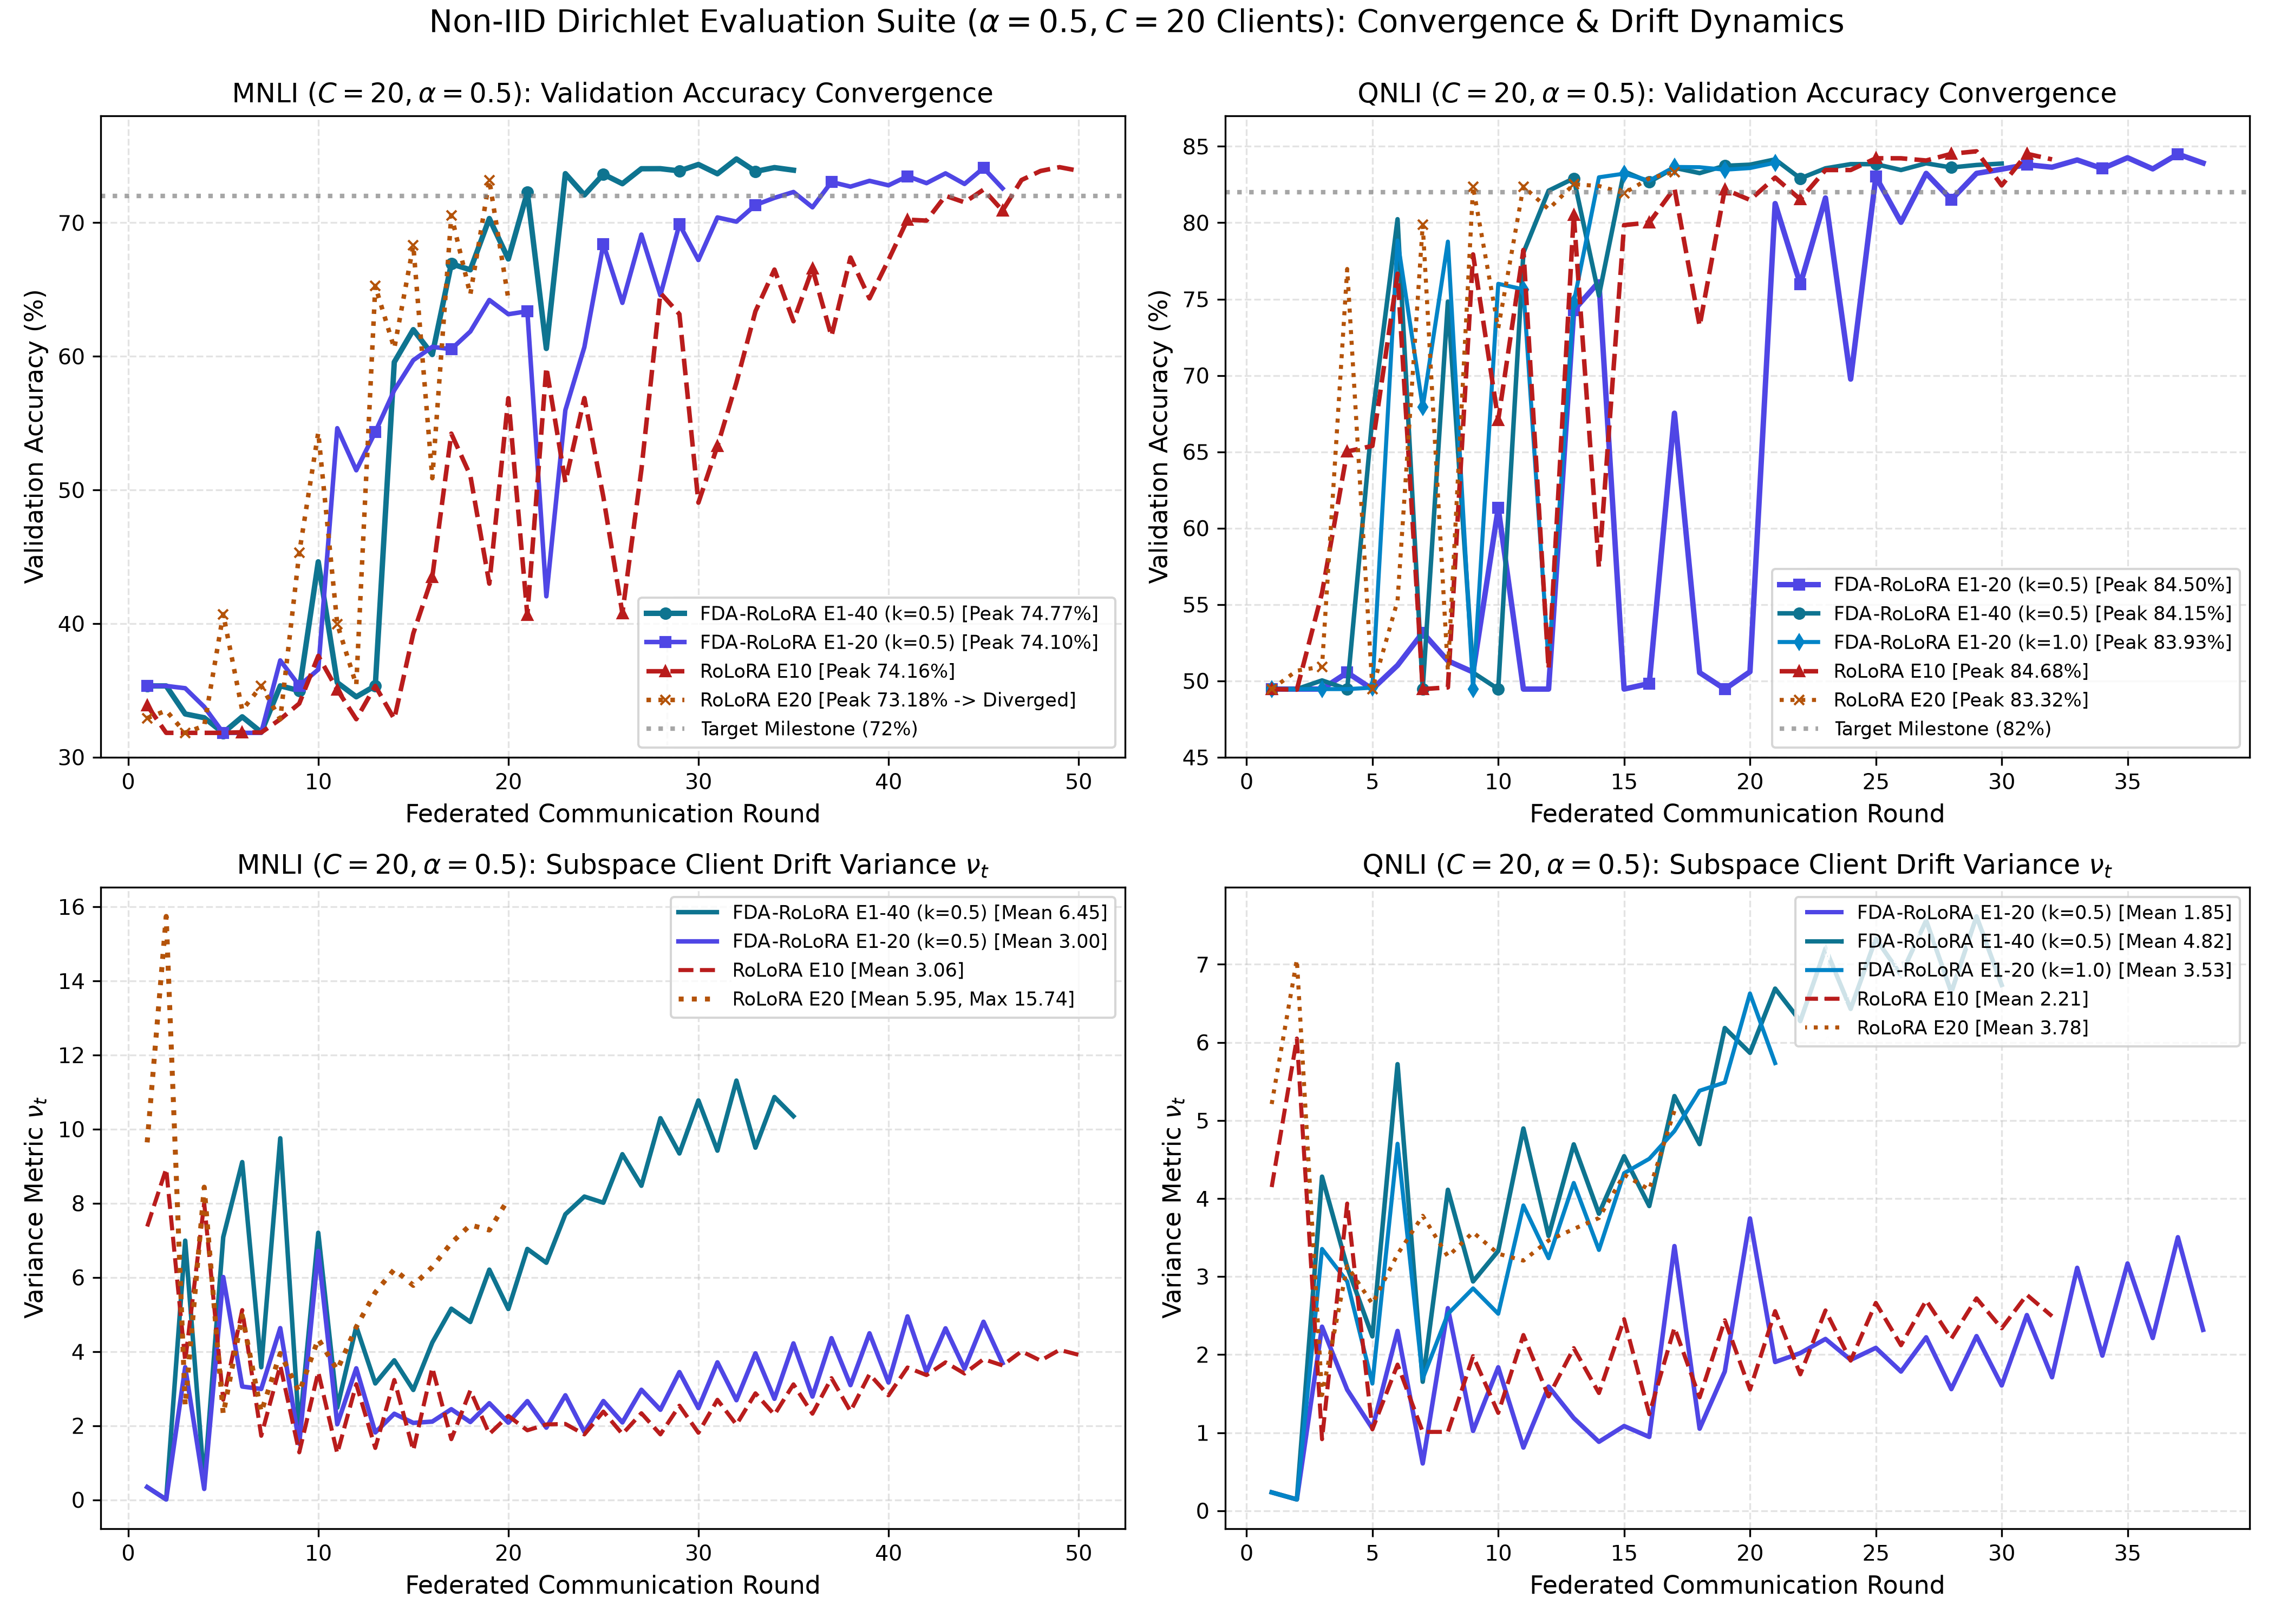
\includegraphics[width=0.95\textwidth]{figures/non_iid_benchmark_telemetry.png}
    \caption{Convergence and client drift variance trajectories on MNLI and QNLI under severe Dirichlet statistical heterogeneity ($\alpha = 0.5$). Top panels present validation accuracy trajectories; bottom panels present client coordinate drift variance ($\sigma_t^2$).}
    \label{fig:non_iid_benchmark_telemetry}
\end{figure}

\clearpage
